% Options for packages loaded elsewhere
\PassOptionsToPackage{unicode}{hyperref}
\PassOptionsToPackage{hyphens}{url}
\PassOptionsToPackage{dvipsnames,svgnames,x11names}{xcolor}
%
\documentclass[
  a4paper,
  DIV=11,
  oneside]{scrreprt}

\usepackage{amsmath,amssymb}
\usepackage{setspace}
\usepackage{iftex}
\ifPDFTeX
  \usepackage[T1]{fontenc}
  \usepackage[utf8]{inputenc}
  \usepackage{textcomp} % provide euro and other symbols
\else % if luatex or xetex
  \usepackage{unicode-math}
  \defaultfontfeatures{Scale=MatchLowercase}
  \defaultfontfeatures[\rmfamily]{Ligatures=TeX,Scale=1}
\fi
\usepackage{lmodern}
\ifPDFTeX\else  
    % xetex/luatex font selection
\fi
% Use upquote if available, for straight quotes in verbatim environments
\IfFileExists{upquote.sty}{\usepackage{upquote}}{}
\IfFileExists{microtype.sty}{% use microtype if available
  \usepackage[]{microtype}
  \UseMicrotypeSet[protrusion]{basicmath} % disable protrusion for tt fonts
}{}
\makeatletter
\@ifundefined{KOMAClassName}{% if non-KOMA class
  \IfFileExists{parskip.sty}{%
    \usepackage{parskip}
  }{% else
    \setlength{\parindent}{0pt}
    \setlength{\parskip}{6pt plus 2pt minus 1pt}}
}{% if KOMA class
  \KOMAoptions{parskip=half}}
\makeatother
\usepackage{xcolor}
\usepackage[inner=3cm,outer=5cm,top=3cm,bottom=4cm,headsep=22pt,headheight=11pt,footskip=33pt,ignorehead,ignorefoot,heightrounded]{geometry}
\setlength{\emergencystretch}{3em} % prevent overfull lines
\setcounter{secnumdepth}{5}
% Make \paragraph and \subparagraph free-standing
\ifx\paragraph\undefined\else
  \let\oldparagraph\paragraph
  \renewcommand{\paragraph}[1]{\oldparagraph{#1}\mbox{}}
\fi
\ifx\subparagraph\undefined\else
  \let\oldsubparagraph\subparagraph
  \renewcommand{\subparagraph}[1]{\oldsubparagraph{#1}\mbox{}}
\fi

\usepackage{color}
\usepackage{fancyvrb}
\newcommand{\VerbBar}{|}
\newcommand{\VERB}{\Verb[commandchars=\\\{\}]}
\DefineVerbatimEnvironment{Highlighting}{Verbatim}{commandchars=\\\{\}}
% Add ',fontsize=\small' for more characters per line
\usepackage{framed}
\definecolor{shadecolor}{RGB}{241,243,245}
\newenvironment{Shaded}{\begin{snugshade}}{\end{snugshade}}
\newcommand{\AlertTok}[1]{\textcolor[rgb]{0.68,0.00,0.00}{#1}}
\newcommand{\AnnotationTok}[1]{\textcolor[rgb]{0.37,0.37,0.37}{#1}}
\newcommand{\AttributeTok}[1]{\textcolor[rgb]{0.40,0.45,0.13}{#1}}
\newcommand{\BaseNTok}[1]{\textcolor[rgb]{0.68,0.00,0.00}{#1}}
\newcommand{\BuiltInTok}[1]{\textcolor[rgb]{0.00,0.23,0.31}{#1}}
\newcommand{\CharTok}[1]{\textcolor[rgb]{0.13,0.47,0.30}{#1}}
\newcommand{\CommentTok}[1]{\textcolor[rgb]{0.37,0.37,0.37}{#1}}
\newcommand{\CommentVarTok}[1]{\textcolor[rgb]{0.37,0.37,0.37}{\textit{#1}}}
\newcommand{\ConstantTok}[1]{\textcolor[rgb]{0.56,0.35,0.01}{#1}}
\newcommand{\ControlFlowTok}[1]{\textcolor[rgb]{0.00,0.23,0.31}{#1}}
\newcommand{\DataTypeTok}[1]{\textcolor[rgb]{0.68,0.00,0.00}{#1}}
\newcommand{\DecValTok}[1]{\textcolor[rgb]{0.68,0.00,0.00}{#1}}
\newcommand{\DocumentationTok}[1]{\textcolor[rgb]{0.37,0.37,0.37}{\textit{#1}}}
\newcommand{\ErrorTok}[1]{\textcolor[rgb]{0.68,0.00,0.00}{#1}}
\newcommand{\ExtensionTok}[1]{\textcolor[rgb]{0.00,0.23,0.31}{#1}}
\newcommand{\FloatTok}[1]{\textcolor[rgb]{0.68,0.00,0.00}{#1}}
\newcommand{\FunctionTok}[1]{\textcolor[rgb]{0.28,0.35,0.67}{#1}}
\newcommand{\ImportTok}[1]{\textcolor[rgb]{0.00,0.46,0.62}{#1}}
\newcommand{\InformationTok}[1]{\textcolor[rgb]{0.37,0.37,0.37}{#1}}
\newcommand{\KeywordTok}[1]{\textcolor[rgb]{0.00,0.23,0.31}{#1}}
\newcommand{\NormalTok}[1]{\textcolor[rgb]{0.00,0.23,0.31}{#1}}
\newcommand{\OperatorTok}[1]{\textcolor[rgb]{0.37,0.37,0.37}{#1}}
\newcommand{\OtherTok}[1]{\textcolor[rgb]{0.00,0.23,0.31}{#1}}
\newcommand{\PreprocessorTok}[1]{\textcolor[rgb]{0.68,0.00,0.00}{#1}}
\newcommand{\RegionMarkerTok}[1]{\textcolor[rgb]{0.00,0.23,0.31}{#1}}
\newcommand{\SpecialCharTok}[1]{\textcolor[rgb]{0.37,0.37,0.37}{#1}}
\newcommand{\SpecialStringTok}[1]{\textcolor[rgb]{0.13,0.47,0.30}{#1}}
\newcommand{\StringTok}[1]{\textcolor[rgb]{0.13,0.47,0.30}{#1}}
\newcommand{\VariableTok}[1]{\textcolor[rgb]{0.07,0.07,0.07}{#1}}
\newcommand{\VerbatimStringTok}[1]{\textcolor[rgb]{0.13,0.47,0.30}{#1}}
\newcommand{\WarningTok}[1]{\textcolor[rgb]{0.37,0.37,0.37}{\textit{#1}}}

\providecommand{\tightlist}{%
  \setlength{\itemsep}{0pt}\setlength{\parskip}{0pt}}\usepackage{longtable,booktabs,array}
\usepackage{calc} % for calculating minipage widths
% Correct order of tables after \paragraph or \subparagraph
\usepackage{etoolbox}
\makeatletter
\patchcmd\longtable{\par}{\if@noskipsec\mbox{}\fi\par}{}{}
\makeatother
% Allow footnotes in longtable head/foot
\IfFileExists{footnotehyper.sty}{\usepackage{footnotehyper}}{\usepackage{footnote}}
\makesavenoteenv{longtable}
\usepackage{graphicx}
\makeatletter
\def\maxwidth{\ifdim\Gin@nat@width>\linewidth\linewidth\else\Gin@nat@width\fi}
\def\maxheight{\ifdim\Gin@nat@height>\textheight\textheight\else\Gin@nat@height\fi}
\makeatother
% Scale images if necessary, so that they will not overflow the page
% margins by default, and it is still possible to overwrite the defaults
% using explicit options in \includegraphics[width, height, ...]{}
\setkeys{Gin}{width=\maxwidth,height=\maxheight,keepaspectratio}
% Set default figure placement to htbp
\makeatletter
\def\fps@figure{htbp}
\makeatother
\newlength{\cslhangindent}
\setlength{\cslhangindent}{1.5em}
\newlength{\csllabelwidth}
\setlength{\csllabelwidth}{3em}
\newlength{\cslentryspacingunit} % times entry-spacing
\setlength{\cslentryspacingunit}{\parskip}
\newenvironment{CSLReferences}[2] % #1 hanging-ident, #2 entry spacing
 {% don't indent paragraphs
  \setlength{\parindent}{0pt}
  % turn on hanging indent if param 1 is 1
  \ifodd #1
  \let\oldpar\par
  \def\par{\hangindent=\cslhangindent\oldpar}
  \fi
  % set entry spacing
  \setlength{\parskip}{#2\cslentryspacingunit}
 }%
 {}
\usepackage{calc}
\newcommand{\CSLBlock}[1]{#1\hfill\break}
\newcommand{\CSLLeftMargin}[1]{\parbox[t]{\csllabelwidth}{#1}}
\newcommand{\CSLRightInline}[1]{\parbox[t]{\linewidth - \csllabelwidth}{#1}\break}
\newcommand{\CSLIndent}[1]{\hspace{\cslhangindent}#1}

\usepackage{booktabs}
\usepackage{longtable}
\usepackage{array}
\usepackage{multirow}
\usepackage{wrapfig}
\usepackage{float}
\usepackage{colortbl}
\usepackage{pdflscape}
\usepackage{tabu}
\usepackage{threeparttable}
\usepackage{threeparttablex}
\usepackage[normalem]{ulem}
\usepackage{makecell}
\usepackage{xcolor}
\usepackage{caption}
\usepackage{lscape}
\newcommand{\blandscape}{\begin{landscape}}
\newcommand{\elandscape}{\end{landscape}}
\usepackage{float}
\floatplacement{table}{t}
\usepackage{amsmath, amssymb, amsthm, amstext}
\usepackage{mlmodern}
\usepackage[T1]{fontenc}
\usepackage{fvextra}
\DefineVerbatimEnvironment{Highlighting}{Verbatim}{breaklines,commandchars=\\\{\}}
\KOMAoption{captions}{tableheading}
\makeatletter
\@ifpackageloaded{tcolorbox}{}{\usepackage[skins,breakable]{tcolorbox}}
\@ifpackageloaded{fontawesome5}{}{\usepackage{fontawesome5}}
\definecolor{quarto-callout-color}{HTML}{909090}
\definecolor{quarto-callout-note-color}{HTML}{0758E5}
\definecolor{quarto-callout-important-color}{HTML}{CC1914}
\definecolor{quarto-callout-warning-color}{HTML}{EB9113}
\definecolor{quarto-callout-tip-color}{HTML}{00A047}
\definecolor{quarto-callout-caution-color}{HTML}{FC5300}
\definecolor{quarto-callout-color-frame}{HTML}{acacac}
\definecolor{quarto-callout-note-color-frame}{HTML}{4582ec}
\definecolor{quarto-callout-important-color-frame}{HTML}{d9534f}
\definecolor{quarto-callout-warning-color-frame}{HTML}{f0ad4e}
\definecolor{quarto-callout-tip-color-frame}{HTML}{02b875}
\definecolor{quarto-callout-caution-color-frame}{HTML}{fd7e14}
\makeatother
\makeatletter
\makeatother
\makeatletter
\@ifpackageloaded{bookmark}{}{\usepackage{bookmark}}
\makeatother
\makeatletter
\@ifpackageloaded{caption}{}{\usepackage{caption}}
\AtBeginDocument{%
\ifdefined\contentsname
  \renewcommand*\contentsname{Inhaltsverzeichnis}
\else
  \newcommand\contentsname{Inhaltsverzeichnis}
\fi
\ifdefined\listfigurename
  \renewcommand*\listfigurename{Abbildungsverzeichnis}
\else
  \newcommand\listfigurename{Abbildungsverzeichnis}
\fi
\ifdefined\listtablename
  \renewcommand*\listtablename{Tabellenverzeichnis}
\else
  \newcommand\listtablename{Tabellenverzeichnis}
\fi
\ifdefined\figurename
  \renewcommand*\figurename{Abbildung}
\else
  \newcommand\figurename{Abbildung}
\fi
\ifdefined\tablename
  \renewcommand*\tablename{Tabelle}
\else
  \newcommand\tablename{Tabelle}
\fi
}
\@ifpackageloaded{float}{}{\usepackage{float}}
\floatstyle{ruled}
\@ifundefined{c@chapter}{\newfloat{codelisting}{h}{lop}}{\newfloat{codelisting}{h}{lop}[chapter]}
\floatname{codelisting}{Listing}
\newcommand*\listoflistings{\listof{codelisting}{Listingverzeichnis}}
\makeatother
\makeatletter
\@ifpackageloaded{caption}{}{\usepackage{caption}}
\@ifpackageloaded{subcaption}{}{\usepackage{subcaption}}
\makeatother
\makeatletter
\@ifpackageloaded{tcolorbox}{}{\usepackage[skins,breakable]{tcolorbox}}
\makeatother
\makeatletter
\@ifundefined{shadecolor}{\definecolor{shadecolor}{rgb}{.97, .97, .97}}
\makeatother
\makeatletter
\makeatother
\makeatletter
\@ifpackageloaded{sidenotes}{}{\usepackage{sidenotes}}
\@ifpackageloaded{marginnote}{}{\usepackage{marginnote}}
\makeatother
\makeatletter
\makeatother
\ifLuaTeX
\usepackage[bidi=basic]{babel}
\else
\usepackage[bidi=default]{babel}
\fi
\babelprovide[main,import]{ngerman}
% get rid of language-specific shorthands (see #6817):
\let\LanguageShortHands\languageshorthands
\def\languageshorthands#1{}
\ifLuaTeX
  \usepackage{selnolig}  % disable illegal ligatures
\fi
\IfFileExists{bookmark.sty}{\usepackage{bookmark}}{\usepackage{hyperref}}
\IfFileExists{xurl.sty}{\usepackage{xurl}}{} % add URL line breaks if available
\urlstyle{same} % disable monospaced font for URLs
\hypersetup{
  pdftitle={Kausalanalyse und Machinelles Lernen mit R},
  pdfauthor={Martin C. Arnold, Christoph Hanck},
  pdflang={de},
  colorlinks=true,
  linkcolor={blue},
  filecolor={Maroon},
  citecolor={Blue},
  urlcolor={Blue},
  pdfcreator={LaTeX via pandoc}}

\title{Kausalanalyse und Machinelles Lernen mit R}
\usepackage{etoolbox}
\makeatletter
\providecommand{\subtitle}[1]{% add subtitle to \maketitle
  \apptocmd{\@title}{\par {\large #1 \par}}{}{}
}
\makeatother
\subtitle{Ein Leitfaden für reproduzierbare Forschung}
\author{Martin C. Arnold, Christoph Hanck}
\date{2023-11-01}

\begin{document}
\maketitle
\RecustomVerbatimEnvironment{verbatim}{Verbatim}{
showspaces = false,
showtabs = false,
breaksymbolleft={},
breaklines
}

\ifdefined\Shaded\renewenvironment{Shaded}{\begin{tcolorbox}[sharp corners, boxrule=0pt, interior hidden, frame hidden, breakable, enhanced, borderline west={3pt}{0pt}{shadecolor}]}{\end{tcolorbox}}\fi

\renewcommand*\contentsname{Inhaltsverzeichnis}
{
\hypersetup{linkcolor=}
\setcounter{tocdepth}{2}
\tableofcontents
}
\setstretch{1.2}
\bookmarksetup{startatroot}

\hypertarget{start}{%
\chapter{Start}\label{start}}

\bookmarksetup{startatroot}

\hypertarget{statistische-programmierung-mit-r}{%
\chapter{Statistische Programmierung mit
R}\label{statistische-programmierung-mit-r}}

Dieses Kapitel ist \emph{nicht} als umfassende Einführung in R gedacht,
sondern behandelt Kernfunktionen aus der Paketsammlung
\texttt{tidyverse}. Wenngleich die Inhalte deutlich über ein
Hallo-Welt-Beispiel\footnote{https://de.wikipedia.org/wiki/Hallo-Welt-Programm}
hinausgehen, betrachten wir hier grundlegene Funktionen für
Datenmanipulation und Visualisierung. Diese sind Vorraussetzung für das
Verständnis fortgeschrittener Code-Bausteine in späteren Kapiteln. Falls
Sie bereits über Grundkenntnisse im Umgang mit \texttt{tidyverse}
verfügen, können Sie dieses Kapitel überspringen. Sollten Sie nicht oder
nur teilweise mit den hier gezeigten Befehlen vertraut sein oder
keinerlei Erfahrung mit R haben, empfiehlt sich vorab eine Erarbeitung
bzw. Wiederholung der Inhalte. Nachstehede Ressourcen finden wir
hilfreich:

\begin{itemize}
\item
  Feedbackgestütze interaktive Übungsaufgaben bei DataCamp\footnote{Ein
    Teil des hier angebotenen Katalogs (exlusive \emph{Einführung in R})
    ist kostenpflichtig.}, bspw.

  \begin{itemize}
  \tightlist
  \item
    \href{https://campus.datacamp.com/courses/einfuhrung-in-r/}{Einführung
    in R}
  \item
    \href{https://www.datacamp.com/courses/introduction-to-data-visualization-with-ggplot2}{Introduction
    to Data Visualization with ggplot2}
  \item
    \href{https://www.datacamp.com/courses/data-manipulation-with-dplyr}{Data
    Manipulation with dplyr}
  \end{itemize}
\item
  Open-source-Literatur wie

  \begin{itemize}
  \tightlist
  \item
    der umfangreiche Leitfaden von
    \href{https://methodenlehre.github.io/einfuehrung-in-R/}{Ellis und
    Mayer (2023)}
  \item
    \href{https://r4ds.hadley.nz/}{R for Data Science}
  \item
    \href{https://rstudio-education.github.io/hopr/}{Hands-On
    Programming with R}
  \end{itemize}
\end{itemize}

Wir laden zunächst die Paketsammlung \texttt{tidyverse}. Für die
Reproduktion mit dem \href{https://www.r-project.org/}{R GUI} oder mit
\href{https://posit.co/download/rstudio-desktop/}{RStudio} muss das
Paket vorab mit \texttt{install.packages()} installiert werden. In den
interaktiven R-Konsolen in diesem Kapitel (und im Rest des Buchs) sind
die benötigten R-Pakete bereits installiert \emph{und} geladen, sofern
nicht anders beschrieben.

\begin{Shaded}
\begin{Highlighting}[]
\CommentTok{\# Paket tidyverse installieren}
\CommentTok{\# install.packages("tidyverse")}

\CommentTok{\# Paket \textquotesingle{}tidyverse\textquotesingle{} laden}
\FunctionTok{library}\NormalTok{(tidyverse)}
\end{Highlighting}
\end{Shaded}

Für das Verständnis von Code-Chunks ist es hilfreich, Zwischenergebnisse
explizit zu evaluieren und in der Konsole auszugeben. Hierfür
umschließen wir häufig Code-Zeilen mit runden Klammern. Der nächste
Chunk illustriert dies für die Variable \texttt{x}.

\begin{Shaded}
\begin{Highlighting}[]
\NormalTok{\# Variable definieren...}
\NormalTok{x \textless{}{-} pi}
\NormalTok{\# ... und evaluieren}
\NormalTok{x}

\NormalTok{\# Äquivalent:}
\NormalTok{(}
\NormalTok{  x \textless{}{-} pi}
\NormalTok{)}
\end{Highlighting}
\end{Shaded}

\hypertarget{lange-weite-und-tidy-datenformate}{%
\section{Lange, weite und ``tidy''
Datenformate}\label{lange-weite-und-tidy-datenformate}}

Wir betrachten den in Tabelle~\ref{tbl-Klausurergebnisse} dargestellten
Datensatz \emph{Klausurergebnisse}.

\hypertarget{tbl-Klausurergebnisse}{}
\begin{longtable}{lrrr}
\caption{\label{tbl-Klausurergebnisse}Datensatz \emph{Klausurergebnisse} }\tabularnewline

\toprule
Name & Mikro & Makro & Mathe \\ 
\midrule\addlinespace[2.5pt]
Tim & NA & $1.3$ & $3$ \\ 
Lena & $1$ & $3$ & NA \\ 
Ricarda & $2$ & $1.7$ & $1.3$ \\ 
Simon & $2.3$ & $3.3$ & NA \\ 
\bottomrule
\end{longtable}

Der Datensatz ist noch nicht in der R-Arbeitsumgebung verfügbar. Mit der
Funktion \texttt{tribble()} können wir
Tabelle~\ref{tbl-Klausurergebnisse} händisch als R-Objekt der Klasse
\texttt{tibble} definieren

\begin{Shaded}
\begin{Highlighting}[]
\NormalTok{\# \textquotesingle{}klasurergebnisse\textquotesingle{} als tibble definieren}
\NormalTok{(}
\NormalTok{  klausurergebnisse \textless{}{-} tribble(}
\NormalTok{    \textasciitilde{}Name,    \textasciitilde{}Mikro, \textasciitilde{}Makro, \textasciitilde{}Mathe,}
\NormalTok{    "Tim",        NA,    1.3,    3.0,}
\NormalTok{    "Lena",      1.0,    3.0,     NA,}
\NormalTok{    "Ricarda",   2.0,    1.7,    1.3,}
\NormalTok{    "Simon",     2.3,    3.3,     NA}
\NormalTok{  )}
\NormalTok{)}
\end{Highlighting}
\end{Shaded}

\texttt{klausurergebnisse} enhält die Klausurnoten der vier Studierenden
(Boebachtungen) spaltenweise \emph{pro Modul}, d.h. die Spaltennamen
\texttt{Mikro}, \texttt{Makro} und \texttt{Mathe} sind Ausprägungen der
Variable \emph{Modul}. Der Datensatz liegt also \emph{nicht} im s.g.
\emph{Tidy-Format} vor.

\begin{tcolorbox}[enhanced jigsaw, colbacktitle=quarto-callout-tip-color!10!white, bottomtitle=1mm, breakable, leftrule=.75mm, opacityback=0, title=\textcolor{quarto-callout-tip-color}{\faLightbulb}\hspace{0.5em}{Tidy-Format}, left=2mm, arc=.35mm, titlerule=0mm, bottomrule=.15mm, opacitybacktitle=0.6, coltitle=black, toptitle=1mm, colback=white, colframe=quarto-callout-tip-color-frame, toprule=.15mm, rightrule=.15mm]

Tidy-Format: Jede Spalte ist \textbf{\emph{eine}} Variable, jede Reihe
ist \textbf{\emph{eine}} Beobachtung und jede Zelle enthält einen
\textbf{\emph{einen}} Wert. Datensätze im Tidy-Format sind häufig lang:
Die Zeilendimension ist größer als die Spaltendimension.

\end{tcolorbox}

Das Tidy-Format ist hilfreich für statistische Analysen mit
\texttt{tidyverse}-Funktionen wie bspw. \texttt{ggplot()}. Wir nutzen
die Funktion \texttt{tidyr::pivot\_longer()}, um
\texttt{klausurergebnisse} ein (langes) Tidy-Format zu transformieren.

\begin{Shaded}
\begin{Highlighting}[]
\NormalTok{\# \textquotesingle{}klausurergebnisse\textquotesingle{} in Tidy{-}Format überführen}
\NormalTok{(}
\NormalTok{  long \textless{}{-} pivot\_longer(}
\NormalTok{    data = klausurergebnisse, }
\NormalTok{    cols = Mikro:Mathe, }
\NormalTok{    names\_to = "Modul", }
\NormalTok{    values\_to = "Note"}
\NormalTok{  )}
\NormalTok{)}
\end{Highlighting}
\end{Shaded}

Beachte, dass die Spalte \texttt{Name} die Zugehörigkeit der
Ausprägungen (\texttt{Note}) jeder Variable (\texttt{Modul}) zu einer
Beobachtung identifiziert. Mit dieser Information können wir den langen
Datensatz wieder in das ursprüngliche (weite) Format zurückführen. Wir
nutzen hierzu \texttt{tidyr::pivot\_wider()}.

\begin{Shaded}
\begin{Highlighting}[]
\NormalTok{\# langes Format in das Ausgangsformat transformieren}
\NormalTok{(}
\NormalTok{  wide \textless{}{-} pivot\_wider(}
\NormalTok{    data = long,}
\NormalTok{    id\_cols = "Name",}
\NormalTok{    names\_from = "Modul", }
\NormalTok{    values\_from = "Note"}
\NormalTok{  )}
\NormalTok{)}
\end{Highlighting}
\end{Shaded}

Wenn die Zuweisung von Zwischenergebnissen in Variablen nicht benötigt
wird, kann eine Verkettung von Funktionsaufrufen die Verständlichkeit
des Codes verbessern. Hierzu wird der
\href{https://magrittr.tidyverse.org/reference/pipe.html}{Pipe-Operator}
\texttt{\%\textgreater{}\%} genutzt. Wir wiederholen die
Transformationen mit den \texttt{tidyr::pivot\_*}-Funktion bei
Verwendung von \texttt{\%\textgreater{}\%}.

\begin{Shaded}
\begin{Highlighting}[]
\NormalTok{\# langes Format mit \%\textgreater{}\%}
\NormalTok{(}
\NormalTok{  long \textless{}{-} klausurergebnisse \%\textgreater{}\% }
\NormalTok{    pivot\_longer(}
\NormalTok{      cols = Mikro:Mathe, }
\NormalTok{      names\_to = "Modul", }
\NormalTok{      values\_to = "Note"}
\NormalTok{    )}
\NormalTok{)}

\NormalTok{\# weites Format mit \%\textgreater{}\%}
\NormalTok{(}
\NormalTok{  wide \textless{}{-} long \%\textgreater{}\% }
\NormalTok{    pivot\_wider(}
\NormalTok{      id\_cols = "Name",}
\NormalTok{      names\_from = "Modul", }
\NormalTok{      values\_from = "Note"}
\NormalTok{    )}
\NormalTok{)}
\end{Highlighting}
\end{Shaded}

Ein Beispiel für den Nachteil des weiten Formats im Umgang mit
\texttt{tidyverse}-Paketen ist die Funktion \texttt{tidyr::drop\_na()}.
Diese entfernt sämtliche \emph{Zeilen} eines Datensatzes, die
\texttt{NA}-Einträge (d.h. fehlende Werte) aufweisen. Beachte, dass
diese Operation im ursprünglichen weiten Format zum Entfernen ganzer
Beobachtungen aus \texttt{wide} führt.

\begin{Shaded}
\begin{Highlighting}[]
\NormalTok{\# NA{-}Einträge aus dem "weiten" Format entfernen}
\NormalTok{wide \%\textgreater{}\% }
\NormalTok{  drop\_na()}
\end{Highlighting}
\end{Shaded}

Im Tidy-Format \texttt{long} hingegen bleiben die übrigen Informationen
betroffener Beobachtungen erhalten.

\begin{Shaded}
\begin{Highlighting}[]
\NormalTok{\# NA{-}Einträge aus dem "langen" Format entfernen}
\NormalTok{long \%\textgreater{}\% }
\NormalTok{  drop\_na()}
\end{Highlighting}
\end{Shaded}

\hypertarget{pinguine-und-pipes}{%
\section{Pinguine und Pipes}\label{pinguine-und-pipes}}

In diesem Abschnitt zeigen wir die Verwendung häufig verwendeter
\texttt{dplyr}-Funktionen (s.g. \emph{Verben}) für die Transformation
von Datensätzen: \texttt{mutate()}, \texttt{select()},
\texttt{filter()},\texttt{summarise()} und \texttt{arrange()}.

Für die Illustration verwenden wir den Datensatz \texttt{penguins} aus
dem R-Paket \texttt{palmerpenguins}. Dieser Datensatz wurde im Zeitraum
2007 bis 2009 von Dr.~Kristen Gorman im Rahmen des \emph{Palmer Station
Long Term Ecological Research Program} zusammengetragen und enthält
Größenmessungen für drei Pinguinarten, die auf den Inseln des
\href{https://en.wikipedia.org/wiki/Palmer_Archipelago}{Palmer-Archipels}
in der Antarktis beobachtet wurden.

\begin{Shaded}
\begin{Highlighting}[]
\CommentTok{\# Paket \textquotesingle{}palmerpenguins\textquotesingle{} installieren}
\CommentTok{\# install.packages("palmerpenguins")}

\CommentTok{\# Paket \textquotesingle{}palmerpenguins\textquotesingle{} laden}
\FunctionTok{library}\NormalTok{(palmerpenguins)}
\end{Highlighting}
\end{Shaded}

Mit \texttt{data()} wird der Datensatz in der Arbeitsumgebung verfügbar
gemacht. Wir nutzen \texttt{glimpse()}, um einen Überblick zu erhalten.

\begin{Shaded}
\begin{Highlighting}[]
\NormalTok{\# Datensatz in der Arbeitsumgebung verfügbar machen}
\NormalTok{data(penguins)}

\NormalTok{\# Übersicht anzeigen lassen}
\NormalTok{glimpse(penguins)}
\end{Highlighting}
\end{Shaded}

\hypertarget{dplyrmutate}{%
\subsection{\texorpdfstring{\texttt{dplyr::mutate()}}{dplyr::mutate()}}\label{dplyrmutate}}

Mit \texttt{mutate()} können bestehende Variablen überschrieben oder
neue Variablen als Funktion bestehender Variablen definiert werden.
\texttt{mutate()} operiert in der Spaltendimension des Datensatz.

Wir definieren eine neue Variable \texttt{body\_mass\_kg} als
Transformation \texttt{body\_mass\_g/1000}.

\begin{Shaded}
\begin{Highlighting}[]
\NormalTok{\# Neue Variable mit Gewicht in Kg definieren}
\NormalTok{penguins \%\textgreater{}\% }
\NormalTok{  mutate(}
\NormalTok{    body\_mass\_kg = body\_mass\_g/1000}
\NormalTok{  ) \%\textgreater{}\%}
\NormalTok{  glimpse()}
\end{Highlighting}
\end{Shaded}

Mit \texttt{across()} kann die dieselbe Operation auf mehrere Variablen
angewendet werden.

Im nachstehenden Beispiel ändern wir den typ (\texttt{type}) der
Variablen \texttt{species}, \texttt{island}, \texttt{sex} und
\texttt{year} zu \texttt{character}.

\begin{Shaded}
\begin{Highlighting}[]
\NormalTok{\# species, island, sex und year in Typ \textquotesingle{}character\textquotesingle{} umwandeln}
\NormalTok{penguins \%\textgreater{}\% }
\NormalTok{  mutate(}
\NormalTok{    across(}
\NormalTok{      c(species, island, sex, year), }
\NormalTok{      .fns = as.character}
\NormalTok{    )}
\NormalTok{  ) \%\textgreater{}\%}
\NormalTok{  glimpse()}
\end{Highlighting}
\end{Shaded}

\texttt{transmute()} ist eine Variante von \texttt{mutate()}, die
lediglich die transformierten Variablen beibehält.

\begin{Shaded}
\begin{Highlighting}[]
\NormalTok{\# Nur transformierte Variablen behalten}
\NormalTok{penguins \%\textgreater{}\% }
\NormalTok{  transmute(}
\NormalTok{    body\_mass\_kg = body\_mass\_g/1000}
\NormalTok{  )}
\end{Highlighting}
\end{Shaded}

\hypertarget{dplyrselect}{%
\subsection{\texorpdfstring{\texttt{dplyr::select()}}{dplyr::select()}}\label{dplyrselect}}

Mit \texttt{select()} werden Variablen aus dem Datensatz ausgewählt.
Dies geschieht entweder über den Variablennamen\ldots{}

\begin{Shaded}
\begin{Highlighting}[]
\NormalTok{\# \textquotesingle{}species\textquotesingle{} auswählen}
\NormalTok{penguins \%\textgreater{}\% }
\NormalTok{  select(species)}
\end{Highlighting}
\end{Shaded}

\ldots{} oder über eine Indexmenge.\footnote{Hilfreich:
  \texttt{dplyr::pull()} selektiert eine Variable und wandelt diese in
  einen Vektor um.}

\begin{Shaded}
\begin{Highlighting}[]
\NormalTok{\# Teilmenge von Variablen per Index auswählen}
\NormalTok{penguins \%\textgreater{}\% }
\NormalTok{  select(}
\NormalTok{    c(1, 2, 3)}
\NormalTok{  )}
\end{Highlighting}
\end{Shaded}

Variablen können anhand eines Muster im Namen selektiert werden. Die
Selektion von \texttt{ends\_with("mm")} bezieht nur Variablen mit Endung
\texttt{mm} im Namen ein:

\begin{Shaded}
\begin{Highlighting}[]
\NormalTok{\# Nur in mm gemessene Variablen auslesen}
\NormalTok{penguins \%\textgreater{}\% }
\NormalTok{  select(}
\NormalTok{    ends\_with("mm")}
\NormalTok{  )}
\end{Highlighting}
\end{Shaded}

Mit \texttt{where()} können wir Variablen aufgrund bestimmter
Eigenschaften ihrer Ausprägungen selektieren.

\begin{Shaded}
\begin{Highlighting}[]
\NormalTok{\# Nur numerische Variablen auswählen}
\NormalTok{penguins \%\textgreater{}\% }
\NormalTok{  select(}
\NormalTok{    where(is.numeric)}
\NormalTok{  )}
\end{Highlighting}
\end{Shaded}

\hypertarget{dplyrfilter}{%
\subsection{\texorpdfstring{\texttt{dplyr::filter()}}{dplyr::filter()}}\label{dplyrfilter}}

Das Verb \texttt{filter()} filtert den Datensatz in der Zeilendimension.
So können Beobachtungen ausgewält werden, deren Merkmalsausprägungen
bestimmte Kriterien erfüllen. Hierzu muss \texttt{filter()} ein
logischer (\texttt{logical}) Ausdruck übergeben werden. Häufig erfolgt
dies über Vergleichsoperatoren.

\begin{Shaded}
\begin{Highlighting}[]
\NormalTok{\# Nur Pinguine mit bill\_length\_mm \textgreater{}= 39}
\NormalTok{penguins \%\textgreater{}\% }
\NormalTok{  filter(}
\NormalTok{    bill\_length\_mm \textgreater{}= 39}
\NormalTok{  )}
\end{Highlighting}
\end{Shaded}

\begin{Shaded}
\begin{Highlighting}[]
\NormalTok{\# Nur Pinguine mit bill\_length\_mm \textless{}= 40}
\NormalTok{penguins \%\textgreater{}\% }
\NormalTok{  filter(}
\NormalTok{    bill\_length\_mm \textless{}= 40}
\NormalTok{  )}
\end{Highlighting}
\end{Shaded}

Oft ist es praktisch, mehrere Kriterien zu kombinieren.

\begin{Shaded}
\begin{Highlighting}[]
\NormalTok{\# Kombinierter Filter {-}{-} Variante 1}
\NormalTok{penguins \%\textgreater{}\% }
\NormalTok{  filter(}
\NormalTok{    bill\_length\_mm \textgreater{}= 39 \& bill\_length\_mm \textless{}= 40}
\NormalTok{  )}
\end{Highlighting}
\end{Shaded}

Analog: komma-getrennte Kriterien werden intern über den Und-Operator
(\texttt{\&}) verknüpft.

\begin{Shaded}
\begin{Highlighting}[]
\NormalTok{\# Kombinierter Filter {-}{-} Variante 2}
\NormalTok{penguins \%\textgreater{}\% }
\NormalTok{  filter(}
\NormalTok{    bill\_length\_mm \textgreater{}= 39, }
\NormalTok{    bill\_length\_mm \textless{}= 40}
\NormalTok{  )}
\end{Highlighting}
\end{Shaded}

Ähnlich wie bei \texttt{select()} verwenden wir häufig nützliche
Funktionen, welche die Interpretation des Codes erleichtern.
\texttt{dplyr::between()} erlaubt filtern innerhalb eines Intervals.

\begin{Shaded}
\begin{Highlighting}[]
\NormalTok{\# Filtern mit Hilfsfunktion}
\NormalTok{penguins \%\textgreater{}\% }
\NormalTok{  filter(}
\NormalTok{    between(}
\NormalTok{      bill\_length\_mm, left = 39, right = 40}
\NormalTok{    )}
\NormalTok{  )}
\end{Highlighting}
\end{Shaded}

Mit diesen Verben sind wir bereits in der Lage, den Datensatz gemäß
folgender Vorschrift zu bereinigen:

\begin{enumerate}
\def\labelenumi{\arabic{enumi}.}
\tightlist
\item
  Entfernen der Maßeinheiten aus den Variablennamen
\item
  Entfernen von Pinguinen mit fehlenden Werten (\texttt{NA})
\item
  Entfernen von Pinguinen mit einem Gewicht \emph{oberhalb} des
  95\%-Stichprobenquantils
\end{enumerate}

\begin{Shaded}
\begin{Highlighting}[]
\NormalTok{\# Schritt 1}
\NormalTok{(}
\NormalTok{  penguins\_cleaned \textless{}{-} penguins \%\textgreater{}\% }
\NormalTok{    rename(}
\NormalTok{      bill\_length = bill\_length\_mm,}
\NormalTok{      bill\_depth  = bill\_depth\_mm,}
\NormalTok{      flipper\_length = flipper\_length\_mm,}
\NormalTok{      body\_mass = body\_mass\_g}
\NormalTok{    )}
\NormalTok{)}
\end{Highlighting}
\end{Shaded}

\begin{Shaded}
\begin{Highlighting}[]
\NormalTok{\# Schritt 2}
\NormalTok{(}
\NormalTok{  penguins\_cleaned \textless{}{-} penguins\_cleaned \%\textgreater{}\%}
\NormalTok{    drop\_na()}
\NormalTok{)}
\end{Highlighting}
\end{Shaded}

\begin{Shaded}
\begin{Highlighting}[]
\NormalTok{\# Schritt 3}
\NormalTok{penguins\_cleaned \%\textgreater{}\% }
\NormalTok{  filter(}
\NormalTok{    body\_mass \textless{} quantile(body\_mass, probs = .95)}
\NormalTok{  ) \%\textgreater{}\%}
\NormalTok{  glimpse()}
\end{Highlighting}
\end{Shaded}

Durch die Verkettung mit \texttt{\%\textgreater{}\%} können wir
sämtliche Schritte für die Bereinigung ohne das Abspeichern von
Zwischenergebnissen durchführen.

\begin{Shaded}
\begin{Highlighting}[]
\NormalTok{\# Verketter Funktionsaufruf für Datensatzbereinigung}
\NormalTok{penguins\_cleaned \textless{}{-} penguins \%\textgreater{}\% }
\NormalTok{  rename(}
\NormalTok{    bill\_length = bill\_length\_mm,}
\NormalTok{    bill\_depth  = bill\_depth\_mm,}
\NormalTok{    flipper\_length = flipper\_length\_mm,}
\NormalTok{    body\_mass = body\_mass\_g}
\NormalTok{  ) \%\textgreater{}\% }
\NormalTok{  drop\_na() \%\textgreater{}\% }
\NormalTok{  filter(}
\NormalTok{    body\_mass \textless{} quantile(body\_mass, .95)}
\NormalTok{  )}

\NormalTok{penguins\_cleaned \%\textgreater{}\% }
\NormalTok{  glimpse()}
\end{Highlighting}
\end{Shaded}

\hypertarget{dplyrsummarise}{%
\subsection{\texorpdfstring{\texttt{dplyr::summarise()}}{dplyr::summarise()}}\label{dplyrsummarise}}

Das Verb \texttt{summarise()} fasst Variablen über Beobachtungen hinweg
zusammen. Der nachstehende Code-Chunk erzeugt eine Tabelle mit
Stichprobenmittelwert und -standardabweichung von
\texttt{flipper\_length\_mm}.\footnote{\texttt{dplyr::summarise()} darf
  nicht mit \texttt{base::summary()} verwechselt werden!} Um zu
vermeiden, dass die Auswertung aufgrund fehlender Werte (\texttt{NA}) in
\texttt{flipper\_length\_mm} scheitert, lassen wir \texttt{NA}s mit
\texttt{na.rm\ =\ TRUE} bei der Berechnung unberücksichtigt (wir
verwenden weiterhin den unbereinigten Datensatz \texttt{penguins}).

\begin{Shaded}
\begin{Highlighting}[]
\NormalTok{\# statistische Zusammenfassung mit \textquotesingle{}summarise()\textquotesingle{}}
\NormalTok{penguins \%\textgreater{}\% }
\NormalTok{  select(flipper\_length\_mm) \%\textgreater{}\% }
\NormalTok{  summarise(}
\NormalTok{    mean = mean(flipper\_length\_mm, na.rm = TRUE), }
\NormalTok{    sd = sd(flipper\_length\_mm, na.rm = TRUE)}
\NormalTok{  )}
\end{Highlighting}
\end{Shaded}

Varianten von \texttt{summarise()} können über mehrere Variablen
angewendet werden. Wir verwenden \texttt{across()} und \texttt{where()},
um lediglich numerische Variablen mit den in der liste definierten
Funktionen zusammenzufassen. Beachte, dass
\texttt{\textbackslash{}(x)\ mean(x)} eine anonyme Funktion definiert.

\begin{Shaded}
\begin{Highlighting}[]
\NormalTok{penguins \%\textgreater{}\% }
\NormalTok{  summarise(}
\NormalTok{    across(}
\NormalTok{      where(is.numeric), }
\NormalTok{      .fns = list(}
\NormalTok{        mean = \textbackslash{}(x) mean(x, na.rm = TRUE), }
\NormalTok{        sd = \textbackslash{}(x) sd(x, na.rm = TRUE)}
\NormalTok{      )}
\NormalTok{    )}
\NormalTok{  ) \%\textgreater{}\%}
\NormalTok{  glimpse()}
\end{Highlighting}
\end{Shaded}

\hypertarget{dplyrarrange}{%
\subsection{\texorpdfstring{\texttt{dplyr::arrange()}}{dplyr::arrange()}}\label{dplyrarrange}}

Mit \texttt{arrange()} können Datensätze in Abhängigkeit der
beobachteten Ausprägungen von Variablen sortiert werden.

\begin{Shaded}
\begin{Highlighting}[]
\NormalTok{\# Datensatz aufsteigend nach \textquotesingle{}body\_mass\_g\textquotesingle{} sortieren}
\NormalTok{penguins \%\textgreater{}\% }
\NormalTok{  arrange(body\_mass\_g)}
\end{Highlighting}
\end{Shaded}

Die Funktion \texttt{dplyr::desc()} kehrt die Reihenfolge zu einer
absteigenden Sortierung um.

\begin{Shaded}
\begin{Highlighting}[]
\NormalTok{\# Absteigende Sortierung nach \textquotesingle{}body\_mass\_g\textquotesingle{}}
\NormalTok{penguins \%\textgreater{}\% }
\NormalTok{  arrange(}
\NormalTok{    desc(body\_mass\_g)}
\NormalTok{  )}
\end{Highlighting}
\end{Shaded}

Komplexe Sortier-Muster werden durch Übergabe von Variablennamen in der
gewünschten Reihenfolge erreicht.

\begin{Shaded}
\begin{Highlighting}[]
\NormalTok{\# Erst Sortierung nach \textquotesingle{}sex\textquotesingle{}, dann gruppenweise absteigend }
\NormalTok{\# nach \textquotesingle{}body\_mass\_g\textquotesingle{} sortieren}
\NormalTok{penguins \%\textgreater{}\% }
\NormalTok{  arrange(}
\NormalTok{    sex, desc(body\_mass\_g)}
\NormalTok{  )}
\end{Highlighting}
\end{Shaded}

\hypertarget{operationen-mit-gruppierten-datensuxe4tzen}{%
\subsection{Operationen mit gruppierten
Datensätzen}\label{operationen-mit-gruppierten-datensuxe4tzen}}

Für manche Transformationen ist eine Gruppierung der Daten hilfreich.
Wir illustrieren nachfolgend die unterschiedlichen Verhaltensweisen
ausgewählter Verben durch Vergleiche von gruppierten und
nicht-gruppierten Anwendungen.

\begin{Shaded}
\begin{Highlighting}[]
\NormalTok{\# Datensatz gruppieren}
\NormalTok{penguins\_grouped \textless{}{-} penguins \%\textgreater{}\% }
\NormalTok{  group\_by(species)}

\NormalTok{\# Datensatz hat nun die Eigenschaft \textquotesingle{}Groups\textquotesingle{}}
\NormalTok{glimpse(penguins\_grouped)}
\end{Highlighting}
\end{Shaded}

\texttt{species} hat drei Ausprägungen. Entsprechend ist
\texttt{penguins\_grouped} nun in drei Gruppen eingeteilt.

Bei gruppierten Datensätzen fasst \texttt{summarise()} die Variablen pro
Guppe zusammen.

\begin{Shaded}
\begin{Highlighting}[]
\NormalTok{\# summarise {-}{-} ungruppiert:}
\NormalTok{penguins \%\textgreater{}\%}
\NormalTok{  summarise(}
\NormalTok{    across(}
\NormalTok{      where(is.numeric), \textbackslash{}(x) mean(x, na.rm = T)}
\NormalTok{      )}
\NormalTok{    )}
\end{Highlighting}
\end{Shaded}

\begin{Shaded}
\begin{Highlighting}[]
\NormalTok{\# summarise {-}{-} gruppiert:    }
\NormalTok{penguins\_grouped \%\textgreater{}\%}
\NormalTok{  summarise(}
\NormalTok{    across(}
\NormalTok{      where(is.numeric), }
\NormalTok{      \textasciitilde{} mean(., na.rm = T)}
\NormalTok{    )}
\NormalTok{  )}
\end{Highlighting}
\end{Shaded}

\texttt{mutate()} definiert bzw. transformiert für jede Gruppe separat.
Im dies zu veranschaulichen, ziehen wir eine Zufallsstichprobe von 10
Pinguinen aus der Datensatz.

\begin{Shaded}
\begin{Highlighting}[]
\NormalTok{\# Zufallsstichprobe generieren}
\NormalTok{set.seed(123)}
\NormalTok{(}
\NormalTok{  penguins\_sample \textless{}{-} penguins \%\textgreater{}\%}
\NormalTok{    slice\_sample(n = 10)  }
\NormalTok{)}
\end{Highlighting}
\end{Shaded}

\begin{Shaded}
\begin{Highlighting}[]
\NormalTok{\# mutate() {-}{-} ungruppiert:}
\NormalTok{penguins\_sample \%\textgreater{}\%}
\NormalTok{  transmute(}
\NormalTok{    mean = mean(bill\_length\_mm)}
\NormalTok{  )}
\end{Highlighting}
\end{Shaded}

Für den ungruppierten Datensatz berechnet \texttt{mutate()} das
Stichprobenmittel von \texttt{bill\_length\_mm} über \emph{alle} zehn
Datenpunkte und weißt diesen Wert jeweils in der Variable \texttt{mean}
zu.

\begin{Shaded}
\begin{Highlighting}[]
\NormalTok{\# mutate() {-}{-} gruppiert}
\NormalTok{penguins\_sample \%\textgreater{}\%}
\NormalTok{  group\_by(species) \%\textgreater{}\%}
\NormalTok{  transmute(}
\NormalTok{    mean = mean(bill\_length\_mm)}
\NormalTok{  )}
\end{Highlighting}
\end{Shaded}

Bei gruppierten Daten berechnet \texttt{mutate()} das Stichprobenmittel
\emph{pro Gruppe} und weist die Mittelwerte entsprechend zu.

\hypertarget{eine-explorative-analyse-mit-ggplot2}{%
\section{\texorpdfstring{Eine explorative Analyse mit
\texttt{ggplot2}}{Eine explorative Analyse mit ggplot2}}\label{eine-explorative-analyse-mit-ggplot2}}

Der bereinigte Datensatz \texttt{penguins\_cleaned} eignet sich gut für
eine graphische Auswertung mit dem R-Paket \texttt{ggplot2}, welches
Bestandteil des \texttt{tidyverse} ist. Nachfolgend untersuchen wir
Zusammenhänge zwischen den Körpermaßen der Pinguine.

Wir erstellen zunächst einen einfachen Punkteplot des Gewichts
(\texttt{body\_mass}) und der Schnabeltiefe (\texttt{bill\_depth}).

\begin{Shaded}
\begin{Highlighting}[]
\NormalTok{\# Punkteplot: body\_mass vs. bill\_depth}
\NormalTok{penguins\_cleaned \%\textgreater{}\%}
\NormalTok{  ggplot(}
\NormalTok{    mapping = aes(}
\NormalTok{      x = body\_mass, }
\NormalTok{      y = bill\_depth}
\NormalTok{    )}
\NormalTok{  ) +}
\NormalTok{  geom\_point()}
\end{Highlighting}
\end{Shaded}

Die Grafik zeigt einen positiven Zusammenhang zwischen dem Gewicht und
der Schnabeltiefe. Als nächstes passen wir den Code so an, dass die
Datenpunkte entsprechend der Art (\texttt{species}) eingefärbt sind.

\begin{Shaded}
\begin{Highlighting}[]
\NormalTok{\# Punkteplot: Farbliche Darstellung verschiedener Arten}
\NormalTok{penguins\_cleaned \%\textgreater{}\%}
\NormalTok{  ggplot(}
\NormalTok{    mapping = aes(}
\NormalTok{      x = body\_mass, }
\NormalTok{      y = bill\_depth, }
\NormalTok{      color = species}
\NormalTok{    )}
\NormalTok{  ) +}
\NormalTok{  geom\_point()}
\end{Highlighting}
\end{Shaded}

Offenbar gibt es deutliche Unterschiede in der (gemeinsamen) Verteilung
von Gewicht und Schnabeltiefe zwischen den verschiedenen Arten.

Um den Zusammenhang zwischen Gewicht und Schnabeltiefe zu untersuchen,
schätzen wir lineare Regressionen
\[body\_mass = \beta_0 + \beta_1 bill\_depth + u\] separat für jede der
drei Pinguinarten mit der KQ-Methode. Anschließend zeichnen wir die
geschätzten Regressionsgeraden ein.

\begin{Shaded}
\begin{Highlighting}[]
\NormalTok{\# Lineare Regression per Art}
\NormalTok{penguins\_cleaned \%\textgreater{}\%}
\NormalTok{  ggplot(}
\NormalTok{    aes(}
\NormalTok{      x = body\_mass, }
\NormalTok{      y = bill\_depth, }
\NormalTok{      color = species}
\NormalTok{    )}
\NormalTok{  ) +}
\NormalTok{  geom\_point() +}
\NormalTok{  geom\_smooth(method = "lm", se = F)}
\end{Highlighting}
\end{Shaded}

Die Schätzungen bekräftigen die Vermutung, dass der lineare Zusammenhang
zwischen Gewicht und Schnabeltiefe sich nicht zwischen den verschiedenen
Pinguinarten unterscheidet: Pinguine der Art \emph{Gentoo} sind im
Mittel schwerer als Pinguine der übrigen Arten, haben jedoch eine
geringere Schnabeltiefe.

Der nachfolgende Code fügt der Grafik eine Regressionsline \emph{über
alle} Arten hinzu. Wir setzen hierbei das Argment
\texttt{inherit\_aes\ =\ FALSE} und legen damit fest, dass die
Regression für \texttt{body\_mass} und \texttt{bill\_depth} ohne
Differenzierung per \texttt{species} durchgeführt wird.

\begin{Shaded}
\begin{Highlighting}[]
\NormalTok{\# Zusatz: Globale Regression}
\NormalTok{penguins\_cleaned \%\textgreater{}\%}
\NormalTok{  ggplot(}
\NormalTok{    mapping = aes(}
\NormalTok{      x = body\_mass, }
\NormalTok{      y = bill\_depth, }
\NormalTok{      color = species}
\NormalTok{    )}
\NormalTok{  ) +}
\NormalTok{  geom\_point() +}
\NormalTok{  geom\_smooth(method = "lm", se = F) +}
\NormalTok{  \# Regression für alle Datenpunkte}
\NormalTok{  geom\_smooth(}
\NormalTok{    mapping = aes(}
\NormalTok{      x = body\_mass, }
\NormalTok{      y = bill\_depth}
\NormalTok{    ),}
\NormalTok{    method = "lm", }
\NormalTok{    se = F, }
\NormalTok{    inherit.aes = F}
\NormalTok{  )}
\end{Highlighting}
\end{Shaded}

Offenbar ist die vorherige Analyse per Spezies sinnvoller: Die
Regression über alle Arten suggeriert einen negativen Zusammenhang
zwischen Gewicht und Schnabeltiefe.

\emph{Facetting} mit \texttt{facet\_wrap()} erlaubt eine Untersuchung
des Zusammenhangs je Insel (\texttt{island}), auf der die Messung
erfolgt ist.

\begin{Shaded}
\begin{Highlighting}[]
\NormalTok{\# Facettierung des per In}
\NormalTok{penguins\_cleaned \%\textgreater{}\%}
\NormalTok{  ggplot(}
\NormalTok{    mapping = aes(}
\NormalTok{      x = body\_mass, }
\NormalTok{      y = bill\_depth, }
\NormalTok{      color = species)}
\NormalTok{  ) +}
\NormalTok{  geom\_point() +}
\NormalTok{  geom\_smooth(method = "lm", se = F) +}
\NormalTok{  facet\_wrap(\textasciitilde{} island)}
\end{Highlighting}
\end{Shaded}

Wir sehen, dass es hinsichtlich des Zusammenhangs von Gewicht und
Schnabeltiefe keine wesentlichen Diskrepanzen zwischen den drei Inseln
gibt. Darüber hinaus lässt sich anhand der Facetten leicht erkennen, wie
die drei Arten über die Inseln verteilt sind.

\bookmarksetup{startatroot}

\hypertarget{matching}{%
\chapter{Matching}\label{matching}}

\begin{Shaded}
\begin{Highlighting}[]
\NormalTok{\#| context: setup}
\NormalTok{\# create dataset directory}
\NormalTok{dir.create("datasets")}
\NormalTok{\# Download the dataset}
\NormalTok{download.file(}
\NormalTok{    "https://raw.githubusercontent.com/mca91/kasa\_data/main/darkmode.csv",}
\NormalTok{    \textquotesingle{}datasets/darkmode.csv\textquotesingle{}}
\NormalTok{)}
\end{Highlighting}
\end{Shaded}

\hypertarget{einfluss-von-darkmode-auf-blog-lesezeit}{%
\section{Einfluss von Darkmode auf
Blog-Lesezeit}\label{einfluss-von-darkmode-auf-blog-lesezeit}}

\begin{figure}

{\centering 

\begin{figure}[H]

{\centering 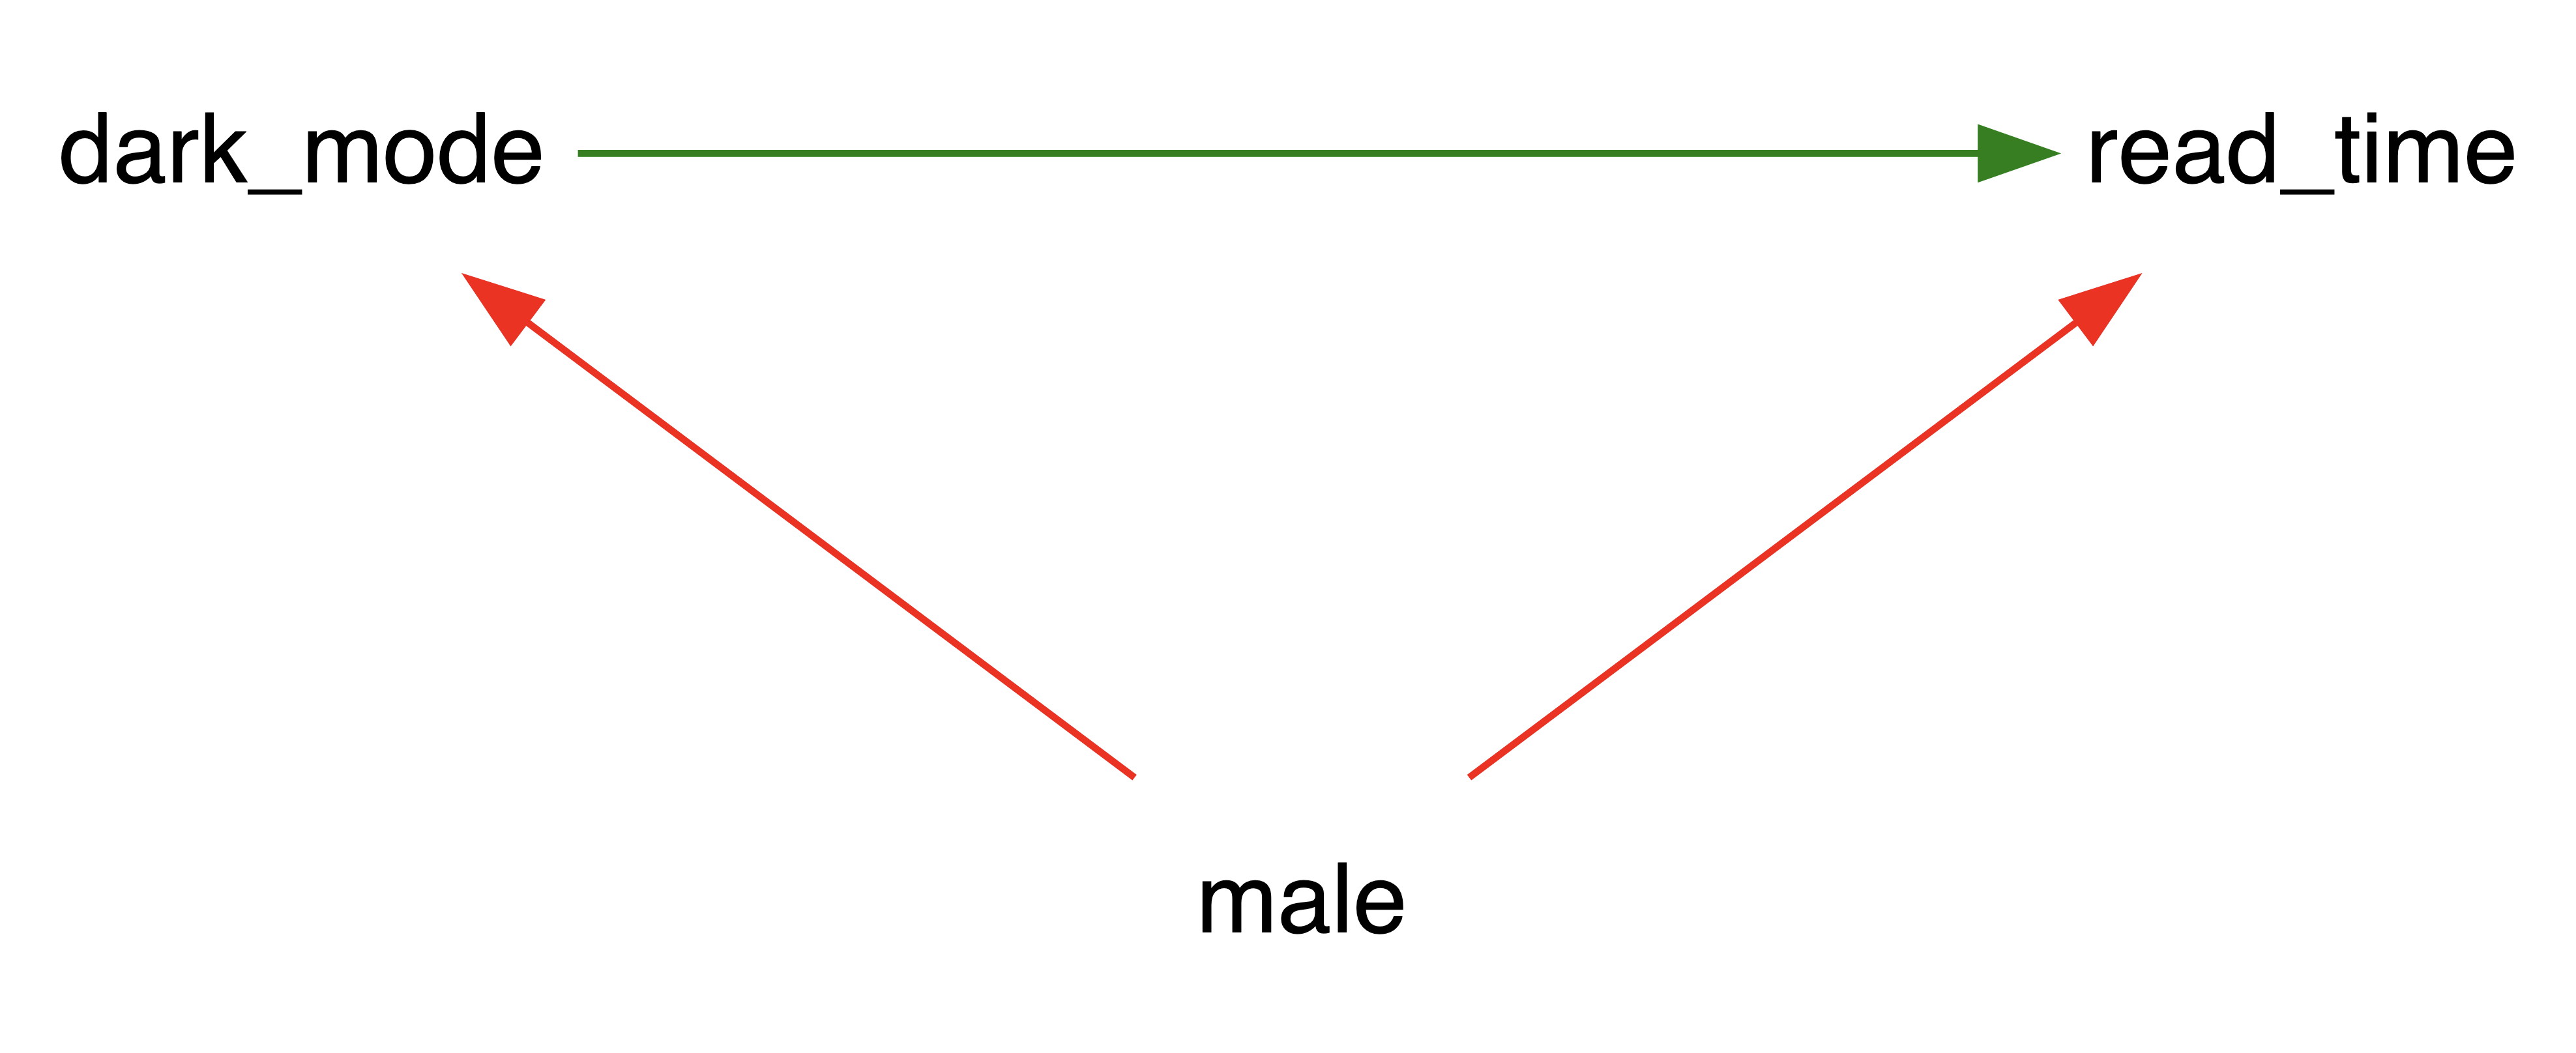
\includegraphics[width=4in,height=3in]{Matching_files/figure-latex/dot-figure-1.png}

}

\end{figure}

}

\caption{\label{fig-CDdarkmode}Geschlecht ist Backdoor-Pfad}

\end{figure}

Wir lesen zunächst den Datensatz \emph{darkmode.csv} ein und verschaffen
uns einen Überblick über die verfügbaren Variablen.

\begin{Shaded}
\begin{Highlighting}[]
\NormalTok{library(tidyverse)}

\NormalTok{\# Datensatz \textquotesingle{}darkmode\textquotesingle{} einlesen}
\NormalTok{darkmode \textless{}{-} read\_csv(}
\NormalTok{  file = "datasets/darkmode.csv", }
\NormalTok{  show\_col\_types = F}
\NormalTok{)}

\NormalTok{\# Überblick verschaffen}
\NormalTok{glimpse(darkmode)}
\end{Highlighting}
\end{Shaded}

\texttt{dark\_mode} hat den Typ \texttt{logical}. Mit
\texttt{dplyr::mutate\_all()} können wir komfortabel alle Spalten in den
Typ \texttt{numeric} transformieren.

\begin{Shaded}
\begin{Highlighting}[]
\NormalTok{\# Alle Variablen zu typ \textquotesingle{}numeric\textquotesingle{} formatieren...}
\NormalTok{darkmode \textless{}{-} darkmode \%\textgreater{}\% }
\NormalTok{  mutate\_all(.funs = as.numeric)}

\NormalTok{\# ... und überprüfen}
\NormalTok{glimpse(darkmode)}
\end{Highlighting}
\end{Shaded}

\begin{figure}

{\centering 

\begin{figure}[H]

{\centering 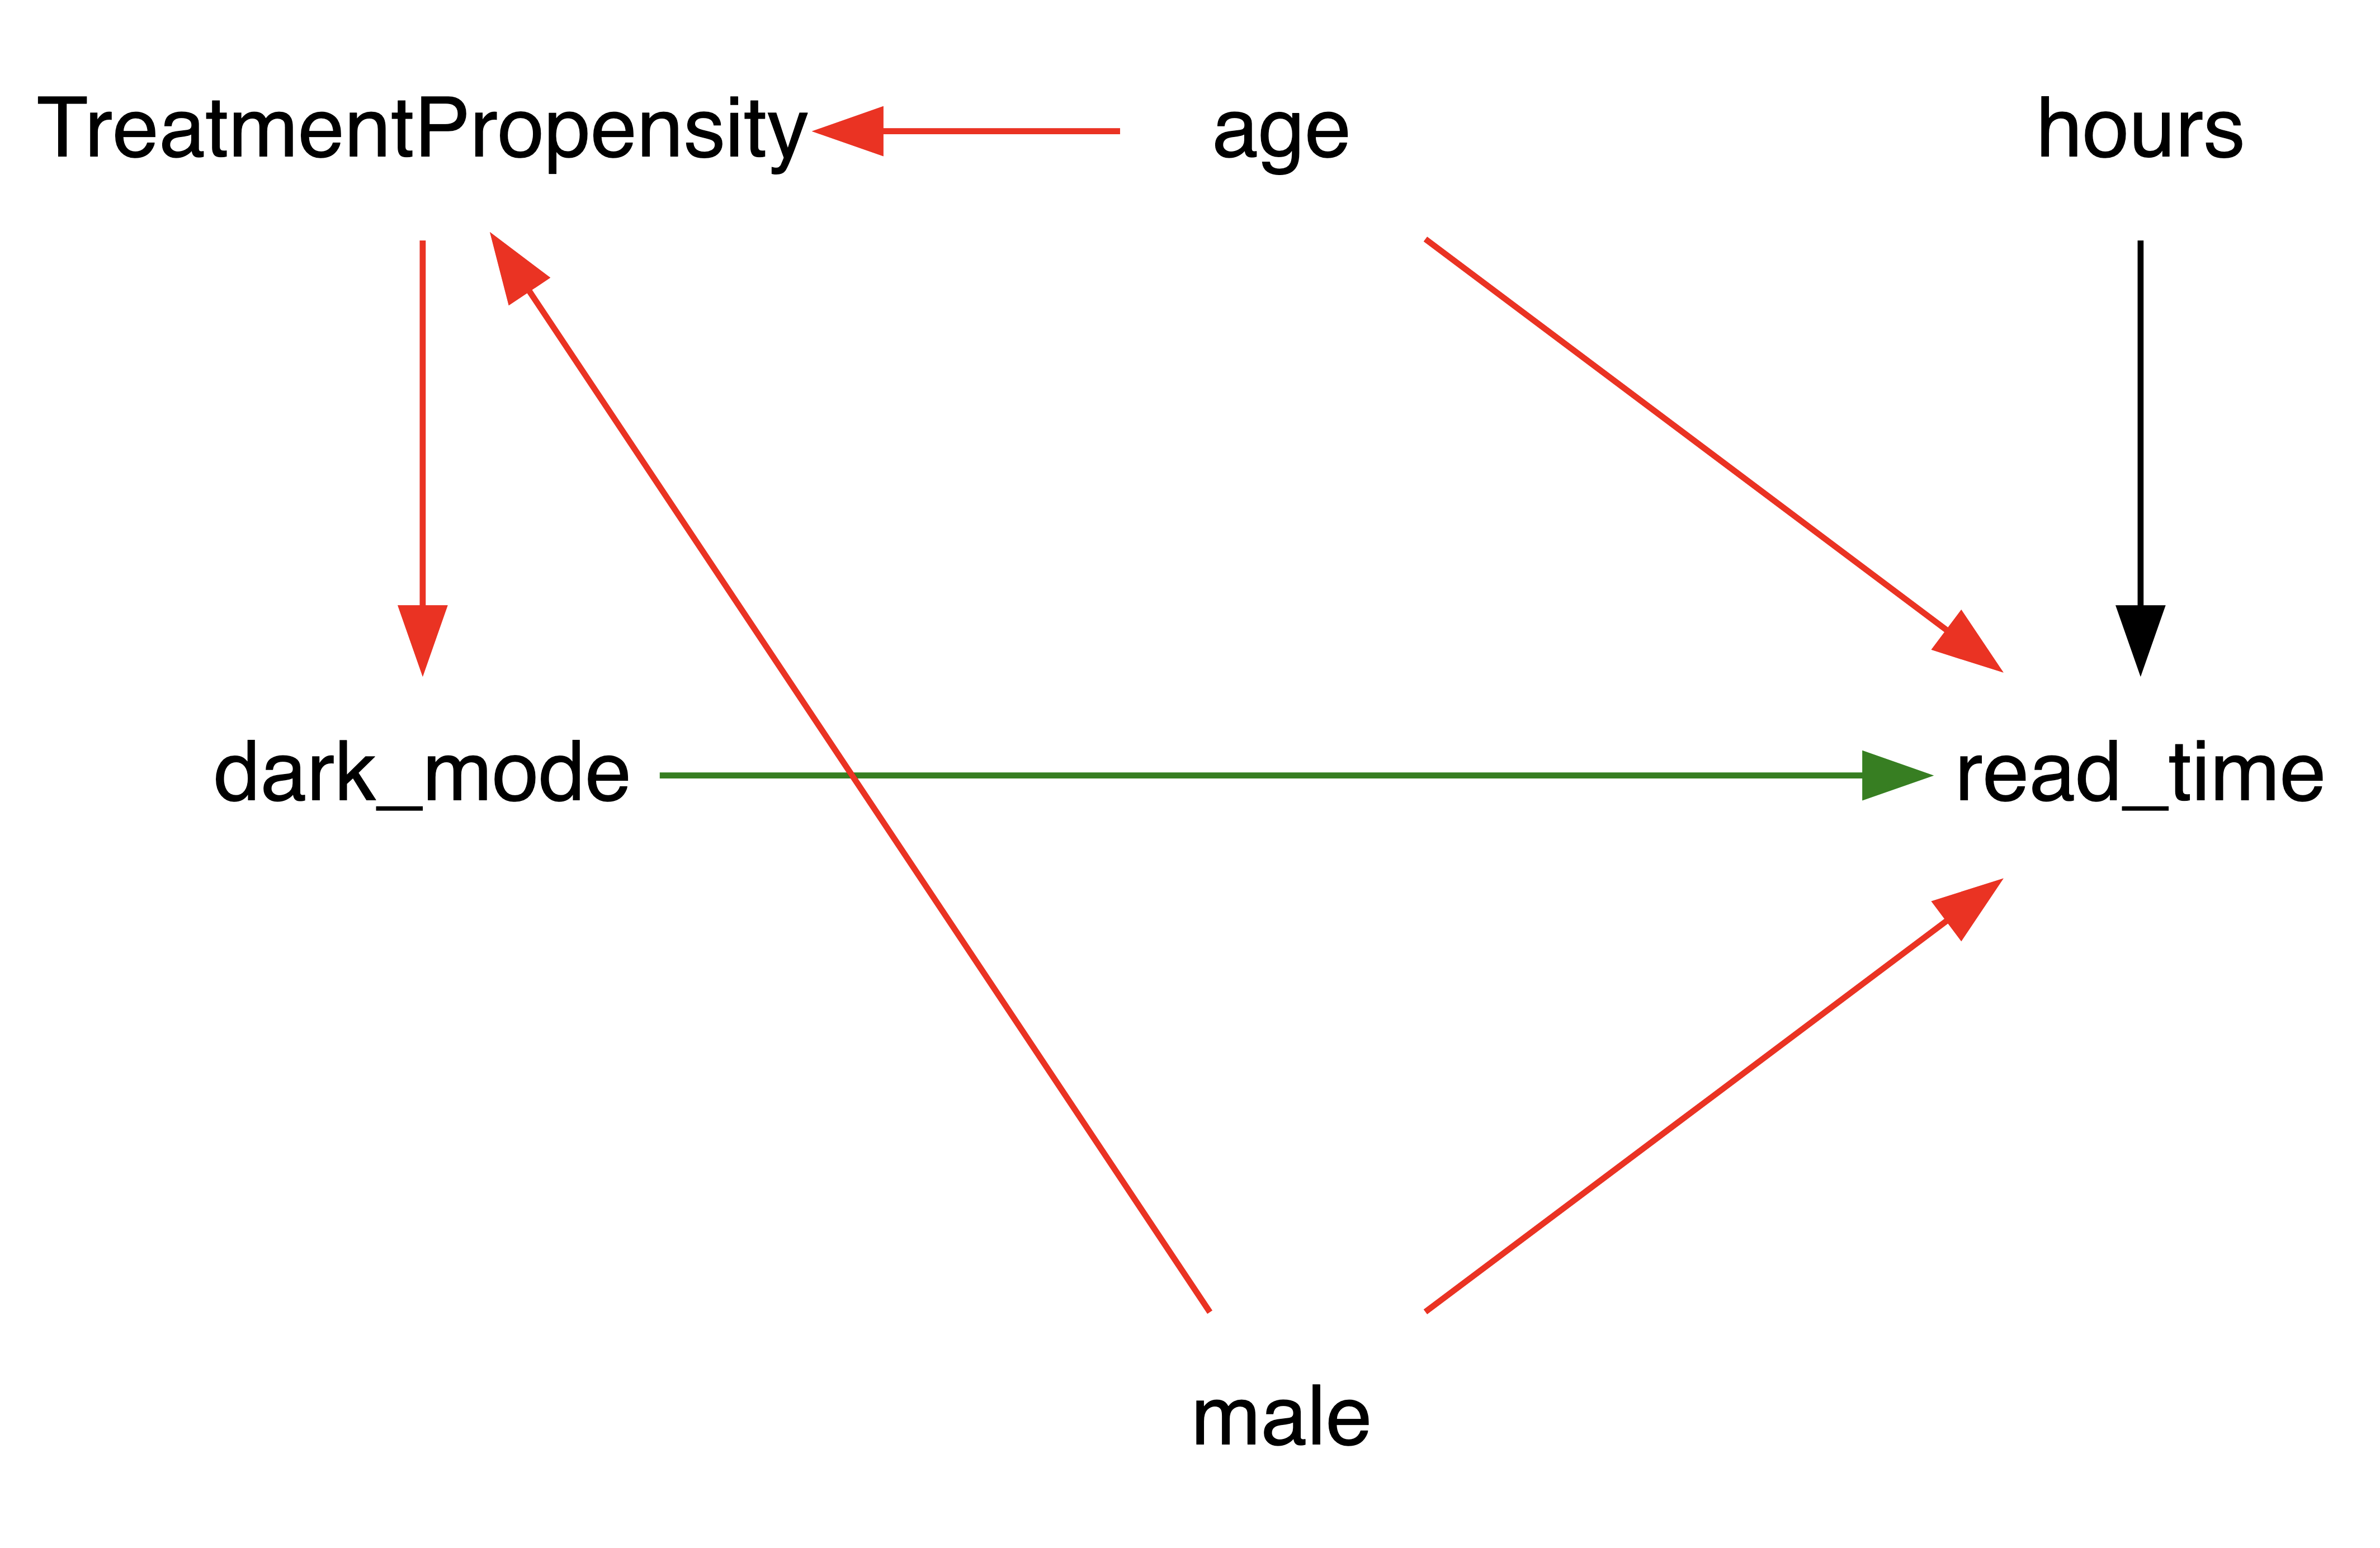
\includegraphics[width=4in,height=3in]{Matching_files/figure-latex/dot-figure-2.png}

}

\end{figure}

}

\caption{\label{fig-CDdarkmode2}Möglicher DGP als Kausales Diagramm}

\end{figure}

\begin{Shaded}
\begin{Highlighting}[]
\NormalTok{\# Logit{-}Modell mit \textquotesingle{}glm()\textquotesingle{} schätzen}
\NormalTok{(}
\NormalTok{  darkmode\_ps\_logit \textless{}{-} glm(}
\NormalTok{    formula = dark\_mode \textasciitilde{} age + male + hours,}
\NormalTok{    data = darkmode,}
\NormalTok{    family = binomial}
\NormalTok{  )}
\NormalTok{)}
\end{Highlighting}
\end{Shaded}

\begin{Shaded}
\begin{Highlighting}[]
\NormalTok{\# Datensatz um propensity scores erweitern}
\NormalTok{(}
\NormalTok{  darkmode\_probabilities \textless{}{-} }
\NormalTok{    darkmode \%\textgreater{}\%}
\NormalTok{    mutate(}
\NormalTok{      propensity = fitted(darkmode\_ps\_logit)}
\NormalTok{    )}
\NormalTok{)}
\end{Highlighting}
\end{Shaded}

Inverse probability weights (IPWs) anhand der PS können schnell anhand
der Vorschrift
\[\texttt{ipw} = \texttt{dark\_mode} / \texttt{propensity} + (1 - \texttt{dark\_mode}) / (1 - \texttt{propensity}), \quad \texttt{dark\_mode} \in\{0,1\}\]
berechnet werden.

\begin{Shaded}
\begin{Highlighting}[]
\NormalTok{\# Datensatz um IPWs erweitern}
\NormalTok{darkmode\_ipw \textless{}{-} darkmode\_probabilities \%\textgreater{}\%}
\NormalTok{  mutate(}
\NormalTok{    ipw = dark\_mode / propensity + (1 {-} dark\_mode) / (1 {-} propensity)}
\NormalTok{  )}

\NormalTok{darkmode\_ipw \%\textgreater{}\% }
\NormalTok{  select(ipw)}
\end{Highlighting}
\end{Shaded}

Verteilung der Propensity Scores nach Behandlungs-Indikator:

\begin{Shaded}
\begin{Highlighting}[]
\NormalTok{\# Dichteschätzung der PS nach Treatment{-}Indikator}
\NormalTok{darkmode\_ipw \%\textgreater{}\%}
\NormalTok{ggplot(}
\NormalTok{  mapping = aes(}
\NormalTok{    x = propensity, }
\NormalTok{    fill = factor(dark\_mode))}
\NormalTok{  ) + }
\NormalTok{  lims(x = c(0, 1)) +}
\NormalTok{  geom\_density(alpha = .5, )}
\end{Highlighting}
\end{Shaded}

Beobachtungen aus der Kontroll-Gruppe entfernen, die außerhalb des
Supports der Treatment-Gruppe liegen.

\begin{Shaded}
\begin{Highlighting}[]
\NormalTok{\# Propensity scores auslesen}
\NormalTok{darkmode\_ipws \textless{}{-} darkmode\_ipw \%\textgreater{}\% }
\NormalTok{  filter(dark\_mode == 1) \%\textgreater{}\% }
\NormalTok{  pull(propensity)}

\NormalTok{\# Support sicherstellen }
\NormalTok{\# (entfernt 13 Beobachtungen aus der Kontrollgruppe)}
\NormalTok{darkmode\_ipw \textless{}{-} darkmode\_ipw \%\textgreater{}\% }
\NormalTok{  filter(}
\NormalTok{    between(}
\NormalTok{      propensity,}
\NormalTok{      darkmode\_ipws \%\textgreater{}\% }
\NormalTok{        min(),}
\NormalTok{      darkmode\_ipws \%\textgreater{}\% }
\NormalTok{        max()}
\NormalTok{    )}
\NormalTok{  )}
\end{Highlighting}
\end{Shaded}

Die Abdeckung können wir erneut mit einer Grafik geschätzter
Dichtefunktionen vergleichen.

\begin{Shaded}
\begin{Highlighting}[]
\NormalTok{\# Dichteschätzung der PS per Treatment{-}Indikator nach Anpassung}
\NormalTok{darkmode\_ipw \%\textgreater{}\%}
\NormalTok{  ggplot(}
\NormalTok{    mapping = aes(}
\NormalTok{      x = propensity, }
\NormalTok{      fill = factor(dark\_mode)}
\NormalTok{    )}
\NormalTok{  ) + }
\NormalTok{  lims(x = c(0, 1)) +}
\NormalTok{  geom\_density(alpha = .5)}
\end{Highlighting}
\end{Shaded}

Wir finden etwas weniger Wahrscheinlichkeits-Masse nahe 0 für die
Kontroll-Gruppe nach filtern von (Kontroll-)Beobachtungen mit PS in der
Spannweite der PS in der Behandlungs-Gruppe. Als nächstes schätzen wir
den ATE mit linearer Regression.

\begin{Shaded}
\begin{Highlighting}[]
\NormalTok{\# Mit IPWs gewichteter KQ{-}Schaetzer berechnet einen ATE}
\NormalTok{model\_ipw \textless{}{-} lm(}
\NormalTok{  formula = read\_time \textasciitilde{} dark\_mode, }
\NormalTok{  data = darkmode\_ipw,}
\NormalTok{  weights = ipw}
\NormalTok{)}

\NormalTok{summary(model\_ipw)}
\end{Highlighting}
\end{Shaded}

Unsere Schätzung des ATE ist der geschätzte Koeffizient von
\texttt{dark\_mode}. Die ausgegebenen Standardfehler und
Inferenzstatistiken sind \emph{ungültig} aufgrund der Gewichtung mit
IPWs, inversen \emph{geschätzten} Wahrscheinlichkeiten für eine
Behandlung. Der Grund hierfür ist, dass die Standardformel in
\texttt{summary()} die zusätzliche Unsicherheit durch die IPW-Schätzung
nicht berücksichtigt!

Die Vergleichbarkeit der Nutzer in Kontroll- und
Behandlungsgruppe-Gruppe für die Variablen \texttt{age}, \texttt{hours}
und \texttt{male} können wir graphisch und anhand einer \emph{balance
table} vergleichen.

\begin{Shaded}
\begin{Highlighting}[]
\NormalTok{\# Dichteschätzungen}
\NormalTok{darkmode \%\textgreater{}\% }
\NormalTok{  group\_by(dark\_mode) \%\textgreater{}\%}
\NormalTok{  select(age, hours) \%\textgreater{}\%}
\NormalTok{  mutate\_all(scale) \%\textgreater{}\% \# Standardisierung mit \textquotesingle{}scale()\textquotesingle{}}
\NormalTok{  pivot\_longer(cols = c({-}dark\_mode)) \%\textgreater{}\% \# langes Format}
  
\NormalTok{  ggplot(aes(x = value, fill = as.factor(dark\_mode))) +}
\NormalTok{  geom\_density( alpha = .5) + }
\NormalTok{  facet\_wrap(\textasciitilde{} name, scales = "free", nrow = 3) \# Facetting nach \textquotesingle{}name\textquotesingle{}}

\NormalTok{\# Relative Hfkt. für \textquotesingle{}male\textquotesingle{} als barplot}
\NormalTok{darkmode \%\textgreater{}\% }
\NormalTok{  group\_by(dark\_mode) \%\textgreater{}\%}
\NormalTok{  mutate(}
\NormalTok{    male = as.factor(male), }
\NormalTok{    dark\_mode = as.factor(dark\_mode)}
\NormalTok{  ) \%\textgreater{}\%}
  
\NormalTok{  ggplot(aes(x = dark\_mode, fill = male)) +}
\NormalTok{  geom\_bar(position = "fill") +}
\NormalTok{  ylab("Anteil")}

\NormalTok{\# Balance table mit \textquotesingle{}cobalt::bal.tab()\textquotesingle{}}
\NormalTok{bal.tab(}
\NormalTok{  x = darkmode \%\textgreater{}\% }
\NormalTok{    select(age, hours, male), }
\NormalTok{  treat = darkmode$dark\_mode, }
\NormalTok{  disp = "m", \# zeige zusätzlich Mittelwerte für C und T}
\NormalTok{)}
\end{Highlighting}
\end{Shaded}

Wir zeigen als nächstes, wie \texttt{MatchIt::matchit()} für
Nearest-neighbor-Matching anhand der Regressoren \texttt{age},
\texttt{hours}, und \texttt{male} in unterschiedlichen Varianten
durchgeführt werden kann.

\texttt{MatchIt::matchit()} führt standardmäßig 1:1-Matching (ohne
Zurücklegen) von Beobachtungen der Treatment-Gruppe mit Beobachtungen
der Kontrollgruppe druch. Das Objekt wird für eine Schätzung des ATT mit
einer geeigneten Funktionen vorbereitet, s. \texttt{?matchit}, und hier
insb. die Argumente \texttt{replace\ =\ F}, \texttt{ratio\ =\ 1} und
\texttt{estimand\ =\ "ATT"} für Details.

Mit \texttt{cobalt::balt.tab()} erhalten wir eine \emph{balance table}
für den gematchten Datensatz.

\textbf{Exaktes Matching}

\begin{Shaded}
\begin{Highlighting}[]
\NormalTok{res \textless{}{-} matchit(}
\NormalTok{  formula = dark\_mode \textasciitilde{} age + male + hours, }
\NormalTok{  data = darkmode, }
\NormalTok{  method = "exact"}
\NormalTok{)}
\NormalTok{bal.tab(res)}
\end{Highlighting}
\end{Shaded}

\textbf{Eins-zu-Eins-Matching: Mahalanobis-Distanz}

\begin{Shaded}
\begin{Highlighting}[]
\NormalTok{res \textless{}{-} matchit(}
\NormalTok{  formula = dark\_mode \textasciitilde{} age + male + hours, }
\NormalTok{  data = darkmode, }
\NormalTok{  distance = "mahalanobis", }
\NormalTok{  method = "nearest"}
\NormalTok{)}
\NormalTok{bal.tab(res)}
\end{Highlighting}
\end{Shaded}

\textbf{Eins-zu-Eins-Matching: Mahalanobis-Distanz mit Caliper 0.25 für
propensity scores basierend auf logistischer Regression}

\begin{Shaded}
\begin{Highlighting}[]
\NormalTok{res \textless{}{-} matchit(}
\NormalTok{  formula = dark\_mode \textasciitilde{} age + male + hours, }
\NormalTok{  data = darkmode, }
\NormalTok{  distance = "glm", }
\NormalTok{  caliper = .25,}
\NormalTok{  mahvars = \textasciitilde{} age + male + hours}
\NormalTok{)}
\NormalTok{\# (Nur K{-}Beobachtungen mit PS bei Caliper .25 kommen für MHD{-}Matching in betracht.)}
\NormalTok{bal.tab(res)}
\end{Highlighting}
\end{Shaded}

\textbf{4. Eins-zu-Eins-Matching: Propensity scores basierend auf
logistischer Regression mit Caliper 0.25}

\begin{Shaded}
\begin{Highlighting}[]
\NormalTok{res \textless{}{-} matchit(}
\NormalTok{  formula = dark\_mode \textasciitilde{} age + male + hours, }
\NormalTok{  data = darkmode, }
\NormalTok{  method = "nearest", }
\NormalTok{  distance = "glm", }
\NormalTok{  caliper = .25}
\NormalTok{)}
\NormalTok{bal.tab(res)}
\end{Highlighting}
\end{Shaded}

Die Vergleichbarkeit der Nutzer in Kontroll- und Treatment-Gruppe
hinsichtlich der Variablen \texttt{age}, \texttt{hours} und
\texttt{male} können wir graphisch und anhand einer \emph{balance table}
vergleichen. Wir berechnen die balance table mit
\texttt{cobalt::bal.tab()} für den anhand von Variante 4 gematchten
Datensatz.

\begin{Shaded}
\begin{Highlighting}[]
\NormalTok{bal.tab(res, un = T, disp = "m")}

\NormalTok{\# Der gematchte Datensatz enthält Gewichte für die jeweilige }
\NormalTok{\# Subklasse zu denen die Beobachtungen gehören.}
\NormalTok{\#}
\NormalTok{\# Hier 1:1 matching \_ohne\_ Zurücklegen, d.h. sämtliche}
\NormalTok{\# Gewichte sind 1 und wird müssten diese nicht für nachfolgende }
\NormalTok{\# Aufrufe von avg comparisons berücksichtigen.}
\NormalTok{darkmode\_matched \textless{}{-} match.data(res)}

\NormalTok{darkmode\_matched \%\textgreater{}\%}
\NormalTok{  group\_by(dark\_mode) \%\textgreater{}\%}
\NormalTok{  select(age, hours) \%\textgreater{}\%}
\NormalTok{  mutate\_all(scale) \%\textgreater{}\%}
\NormalTok{  pivot\_longer(cols = c({-}dark\_mode)) \%\textgreater{}\%}
  
\NormalTok{  ggplot(aes(x = value, fill = as.factor(dark\_mode))) +}
\NormalTok{  geom\_density( alpha = .5) + }
\NormalTok{  facet\_wrap(\textasciitilde{} name, scales = "free", nrow = 3)}

\NormalTok{darkmode\_matched \%\textgreater{}\% }
\NormalTok{  group\_by(dark\_mode) \%\textgreater{}\%}
\NormalTok{  mutate(}
\NormalTok{    male = as.factor(male), }
\NormalTok{    dark\_mode = as.factor(dark\_mode)}
\NormalTok{  ) \%\textgreater{}\%}
  
\NormalTok{  ggplot(aes(x = dark\_mode, fill = male)) +}
\NormalTok{  geom\_bar(position = "fill") +}
\NormalTok{  ylab("Anteil")}
\end{Highlighting}
\end{Shaded}

Wir beobachten eine bessere Balance bei \texttt{age} und \texttt{hours}.
Am wichtigsten: \texttt{gender} (\texttt{male}) ist nahezu ausgeglichen
für Kontroll- und Treatment-Gruppe!

Wir schätzen nun den ATT von \texttt{dark\_mode} auf \texttt{read\_time}
mit linearer Regression für den gematchten Datensatz aus sowie für den
ursprünglichen Datensatz und berechnen jeweils ein robustes
95\%-Konfidenzintervall für den ATT.

\begin{Shaded}
\begin{Highlighting}[]
\NormalTok{\# ATT mit linearem Modell für ungematchten Datensatz schätzen}
\NormalTok{ATT\_mod\_org \textless{}{-} lm(}
\NormalTok{  formula = read\_time \textasciitilde{} age + male + hours + dark\_mode,}
\NormalTok{  data = darkmode}
\NormalTok{)}
\NormalTok{summary(ATT\_mod\_org)}

\NormalTok{\# ATT mit linearem Modell für gematchten Datensatz schätzen}
\NormalTok{ATT\_mod \textless{}{-} lm(}
\NormalTok{  formula = read\_time \textasciitilde{} age + male + hours + dark\_mode,}
\NormalTok{  data = darkmode\_matched, }
\NormalTok{  weights = weights }
\NormalTok{)}
\NormalTok{\# (weights = 1 für alle Beobachtungen weil wg. 1:1{-}Matching}
\NormalTok{\# nur 2er{-}Paare von Beobachtungen. Hier also vernachlässigbar.}
\NormalTok{\# Andere Gewichtung bei k:1{-}Matching!)}
\NormalTok{summary(ATT\_mod)}
\end{Highlighting}
\end{Shaded}

\textbf{Achtung}: Für Matching-Verfahren (\texttt{ATT\_mod}) sind die
von \texttt{summary()} berechneten Standardfehler (und damit KI,
t-Statistiken und p-Werte) für den ATT \emph{grundsätzlich ungültig} Wir
haben 3 Quellen von Schätzunsicherheit, die bei der Berechnung von
Standardfehlern berücksichtigt werden müssen: Die Schätzung der PS, der
Matching-Prozess und die ``übliche'' Stichproben-Variabilität. Wir
nutzen daher nachfolgende Funktionen gem. Empfehlungen aus der aktuellen
Forschung für Standardfehlerberechnung. S. auch Aufgabe 5 (a).

\begin{Shaded}
\begin{Highlighting}[]
\NormalTok{library(marginaleffects)}

\NormalTok{\# Inferenz Multiple Regression bei ungematchten Beobachtungen}
\NormalTok{\# identisch zu \textquotesingle{}coeftest(ATT\_mod\_org, vcovHC, type = "HC3")\textquotesingle{}}
\NormalTok{avg\_comparisons(}
\NormalTok{  model = ATT\_mod\_org,}
\NormalTok{  variables = "dark\_mode",}
\NormalTok{  vcov = "HC3", \# Heteroskedastie{-}robuster SE}
\NormalTok{  newdata = subset(darkmode, dark\_mode == 1) \# Identifiziert Kontrollgruppe}
\NormalTok{) }

\NormalTok{\# Inferenz Multiple Regression bei \_gematchten\_ Beobachtungen}
\NormalTok{avg\_comparisons(}
\NormalTok{  model = ATT\_mod,}
\NormalTok{  variables = "dark\_mode",}
\NormalTok{  vcov = \textasciitilde{}subclass, \# cluster robust SE \textgreater{} als oben =\textgreater{} mehr Unsicherheit}
\NormalTok{  newdata = subset(darkmode\_matched, dark\_mode == 1),}
\NormalTok{  wts = "weights"  \# = 1}
\NormalTok{)}
\NormalTok{\# ( Weights = 1 wg. 1:1{-}Matching.}
\NormalTok{\# Anzahl subclasses = Anzahl gematchter treatment/control units )}
\end{Highlighting}
\end{Shaded}

\hypertarget{inferenz-fuxfcr-attate-propensity-score-matching-mit-bootstrap}{%
\section{Inferenz für ATT/ATE: Propensity-Score-Matching mit
Bootstrap}\label{inferenz-fuxfcr-attate-propensity-score-matching-mit-bootstrap}}

Bei Matching mit Zurücklegen besteht zusätzliche Unsicherheit durch
Zurücklegen, d.h. Beobachtungen aus der Kontroll-Gruppe können mehrfach
als Match für Beobachtungen aus der Treatment-Gruppe genutzt werden. Mit
\texttt{summary()} berechnete Standardfehler berücksichtigen dies nicht!

Ein Bootstrap-Verfahren generiert mit Resampling (wiederholtes Ziehen
mit Zurücklegen) aus dem Original-Datensatz (viele) künstliche
Datensätze, für die der Schätzer (d.h. das gesamte Verfahren inkl.
Matching!) jeweils berechnet wird. Die Verteilung der so gewonnenen
Bootstrap-Schätzwerte approximiert die wahre, unbekannte
Stichprobenverteilung des Schätzers des Behandlungseffekts. Mit dieser
simulierten Verteilung können wir Inferenz betreiben: Wir können einen
Bootstrap-Punktschätzer des Behandlungseffekts (Stichprobenmittel der
Bootstrap-Schätzungen) sowie Standardfehler (Standardabweichung der der
Bootstrap-Schätzungen) und p-Werte berechnen.

Wir Implementieren nun einen Bootstrap-Schätzer des ATT als
\texttt{R}-Funktion \texttt{boot\_fun()}.

\begin{Shaded}
\begin{Highlighting}[]
\NormalTok{boot\_fun \textless{}{-} function(data, i) \{}
  
\NormalTok{  boot\_data \textless{}{-} data[i, ]}
  
\NormalTok{  \# 1:1 PS Matching \_mit\_ Zurücklegen}
\NormalTok{  match\_res \textless{}{-} matchit(dark\_mode \textasciitilde{} age + hours + male,}
\NormalTok{                       data = boot\_data,}
\NormalTok{                       caliper = .25,}
\NormalTok{                       replace = TRUE) \# Zurücklegen}
  
\NormalTok{  \# Gematchten Datensatz zuweisen}
\NormalTok{  darkmode\_matched \textless{}{-} match.data(match\_res, data = boot\_data)}
  
\NormalTok{  \# Outcome{-}Modell schätzen}
\NormalTok{  ATT\_mod \textless{}{-} lm(}
\NormalTok{    formula = read\_time \textasciitilde{} age + male + hours + dark\_mode,}
\NormalTok{    data = darkmode\_matched, }
\NormalTok{    weights = weights \# hier teilweise \textgreater{} 1 wg. Matching mit Zurücklegen!}
\NormalTok{  )}
  
\NormalTok{  \#  ATT{-}Schätzer auslesen}
\NormalTok{  return(}
\NormalTok{    ATT\_mod$coefficients["dark\_mode"]  }
\NormalTok{  )}
\NormalTok{\}}
\end{Highlighting}
\end{Shaded}

Abadie \& Imbens (2008) zeigen analytisch, dass ein Standard-Bootstrap
bei Matching grundsätzlich ungültig ist: Die unbekannte Varianz der
Stichprobenverteilung des Matching-Schätzers (und damit der
Standardfehler des Schätzers) kann durch den Bootstrap nicht repliziert
werden. Problematisch hierbei sind grundsätzlich zu liberale (d.h. zu
große) mit dem Bootstrap berechnete Standardfehler. Es gibt jedoch
Simulationsnachweise die zeigen, dass Bootstrap-Standardfehler bei
Matching mit Zurücklegen konservativ sind (Bodory et al., 2020), also
tendentiell zu kleine Standardfehler produzieren und damit das
gewünschte nominale Signifikanzniveau eines Bootstrap-Hypothesentests
nicht überschritten wird.

Wir berechnen nun eine Bootstrap-Schätzung des ATT von
\texttt{dark\_mode} auf \texttt{readingtime} sowie den zugehörigen
Standardfehler und ein 95\%-KI mit der zuvor definierten Funktion
\texttt{boot\_fun}.

\begin{Shaded}
\begin{Highlighting}[]
\NormalTok{library("boot")}
\NormalTok{set.seed(4321)}
\NormalTok{boot\_out \textless{}{-} boot(darkmode, boot\_fun, R = 999)}

\NormalTok{boot\_out}
\end{Highlighting}
\end{Shaded}

\begin{Shaded}
\begin{Highlighting}[]
\NormalTok{\# Bootstrap{-}Schätzer für den Treatment{-}Effekt}
\NormalTok{mean(boot\_out$t) }
\NormalTok{\# = mean(t0) + bias = mean(Bootstrap\_samples)}
\NormalTok{\# vgl. \textquotesingle{}t0 = boot\_fun(darkmode, i = 1:1e3)\textquotesingle{}}

\NormalTok{\# Bootstrap{-}Standardfehler}
\NormalTok{sd(boot\_out$t)}

\NormalTok{\# 95\% Bootstrap{-}KI für den Treatment{-}Effekt}
\NormalTok{boot.ci(boot\_out, type = "perc")}
\end{Highlighting}
\end{Shaded}

\hypertarget{doubly-robust-schuxe4tzer-fuxfcr-attate}{%
\section{Doubly-Robust-Schätzer für
ATT/ATE}\label{doubly-robust-schuxe4tzer-fuxfcr-attate}}

Implementieren und berechnen Sie einen Doubly-Robust-Schätzer des ATT
(vgl. Wooldridge, 2010) für den kausalen Effekt in Aufgabe 5.
Vergleichen Sie mit den Ergebnissen der Aufgaben 1 (d), 4 (f) und 5 (d).

\begin{Shaded}
\begin{Highlighting}[]
\NormalTok{\# IPW estimation with regression adjustment}
\NormalTok{ipwra \textless{}{-} function(br, index = 1:nrow(br)) \{}
\NormalTok{    \# slice bootstrapped observations}
\NormalTok{    br \textless{}{-} br \%\textgreater{}\% slice(index)}
    
\NormalTok{    \# estimate and predict propensity score}
\NormalTok{    m \textless{}{-} glm(formula = dark\_mode \textasciitilde{} age + hours + male,}
\NormalTok{             data = br, }
\NormalTok{             family = binomial(link = \textquotesingle{}logit\textquotesingle{}))}
    
\NormalTok{    br \textless{}{-} br \%\textgreater{}\%}
\NormalTok{        mutate(ps = predict(m, type = \textquotesingle{}response\textquotesingle{}))}
    
\NormalTok{    \# trim control observations outside of treated PS range}
\NormalTok{    minps \textless{}{-} br \%\textgreater{}\%}
\NormalTok{        filter(dark\_mode == 1) \%\textgreater{}\%}
\NormalTok{        pull(ps) \%\textgreater{}\%}
\NormalTok{        min(na.rm = TRUE)}
    
\NormalTok{    maxps \textless{}{-} br \%\textgreater{}\%}
\NormalTok{        filter(dark\_mode == 1) \%\textgreater{}\%}
\NormalTok{        pull(ps) \%\textgreater{}\%}
\NormalTok{        max(na.rm = TRUE)}
    
\NormalTok{    \# do the trimming}
\NormalTok{    br \textless{}{-} br \%\textgreater{}\%}
\NormalTok{        filter(ps \textgreater{}= minps \& ps \textless{}= maxps)}
    
\NormalTok{    \# compute IPWs}
\NormalTok{    br \textless{}{-} br \%\textgreater{}\%}
\NormalTok{      mutate(}
\NormalTok{        ipw = case\_when(}
\NormalTok{          dark\_mode == 1 \textasciitilde{} 1 / ps,}
\NormalTok{          dark\_mode == 0 \textasciitilde{} 1 / (1 {-} ps))}
\NormalTok{      )}
    
\NormalTok{    \# Simple \_ATT\_ estimate:}
\NormalTok{    \# w\_means \textless{}{-} br \%\textgreater{}\%}
\NormalTok{    \#     group\_by(dark\_mode) \%\textgreater{}\%}
\NormalTok{    \#     summarize(m = weighted.mean(read\_time, w = ipw)) \%\textgreater{}\% }
\NormalTok{    \#     arrange(dark\_mode)}
\NormalTok{    \# }
\NormalTok{    \# \# simple diff{-}in{-}means \_ATT\_ estimate}
\NormalTok{    \#  return(w\_means$m[2] {-} w\_means$m[1]) }
    
\NormalTok{    \# Do regression adjustment for \_ATE\_ estimate}
\NormalTok{    \# TE prediction for whole sample based on TG model}
\NormalTok{    mtreat \textless{}{-} br \%\textgreater{}\%}
\NormalTok{      filter(dark\_mode == 1) \%\textgreater{}\%}
\NormalTok{      lm(read\_time \textasciitilde{} 1 + age + hours + male, data = ., weights = .$ipw) \%\textgreater{}\%}
\NormalTok{      predict(newdata = br) \%\textgreater{}\%}
\NormalTok{      mean()}
    
\NormalTok{    \# TE prediction for whole sample based on CG model}
\NormalTok{    mcont \textless{}{-} br \%\textgreater{}\%}
\NormalTok{      filter(dark\_mode == 0) \%\textgreater{}\%}
\NormalTok{      lm(read\_time \textasciitilde{} 1 + age + hours + male, data = ., weights = .$ipw) \%\textgreater{}\%}
\NormalTok{      predict(newdata = br) \%\textgreater{}\%}
\NormalTok{      mean()}

\NormalTok{    return(mtreat {-} mcont) \# Regression adjusted \_ATE\_ estimate}
\NormalTok{\}}
\end{Highlighting}
\end{Shaded}

\begin{Shaded}
\begin{Highlighting}[]
\NormalTok{b \textless{}{-} boot(data = darkmode, ipwra, R = 999)}
\NormalTok{\# Bootstrap estimate and standard error}
\NormalTok{mean(b$t)}
\NormalTok{sd(b$t)}
\end{Highlighting}
\end{Shaded}

\vfill

\bookmarksetup{startatroot}

\hypertarget{literatur}{%
\chapter{Literatur}\label{literatur}}

Abadie, Alberto, and Guido W. Imbens. (2008). \emph{On the Failure of
the Bootstrap for Matching Estimators.}Econometrica 76 (\textbf{6}):
1537--57.

Bodory, H., Camponovo, L., Huber, M., \& Lechner, M. (2020). \emph{The
Finite Sample Performance of Inference Methods for Propensity Score
Matching and Weighting Estimators}. Journal of Business \& Economic
Statistics, 38(\textbf{1}), 183--200.

Wooldridge, J. M. (2010). \emph{Econometric analysis of cross section
and panel data}. MIT press.

\bookmarksetup{startatroot}

\hypertarget{regression-discontiniuty-designs}{%
\chapter{Regression Discontiniuty
Designs}\label{regression-discontiniuty-designs}}

Regression Discontinuity Design (RDD) ist ein Ansatz für die Schätzung
von Behandlungseffekten mit Regression, wenn durch einen experimentell
oder natürlich gegebenen Umstand die Behandlung an einem Schwellenwert
(\(c\)) einer \emph{Laufvariable} (\(X\)) sprunghaft beeinflusst wird.
Ein RDD-Schätzer wird so implementiert, dass lediglich Beobachtungen mit
Ausprägungen von \(X\), die knapp ober- oder knapp unterhalb von \(c\)
liegen, berücksichtigt werden. Die zentrale Idee hierbei ist, dass
Individuen nahe bei \(c\) im Durchschnitt ähnliche Merkmale aufweisen.
Beobachtungen nahe \(c\) sind dann insbesondere hinsichtlich
potentieller Backdoor-Variablen vergleichbar, sodass deren
problematische Pfade geschlossen sind. Das kausale Diagram in
Abbildung~\ref{fig-CDRDD} zeigt den grundsätzlichen Zusammenhang.

\begin{figure}

{\centering 

\begin{figure}[H]

{\centering 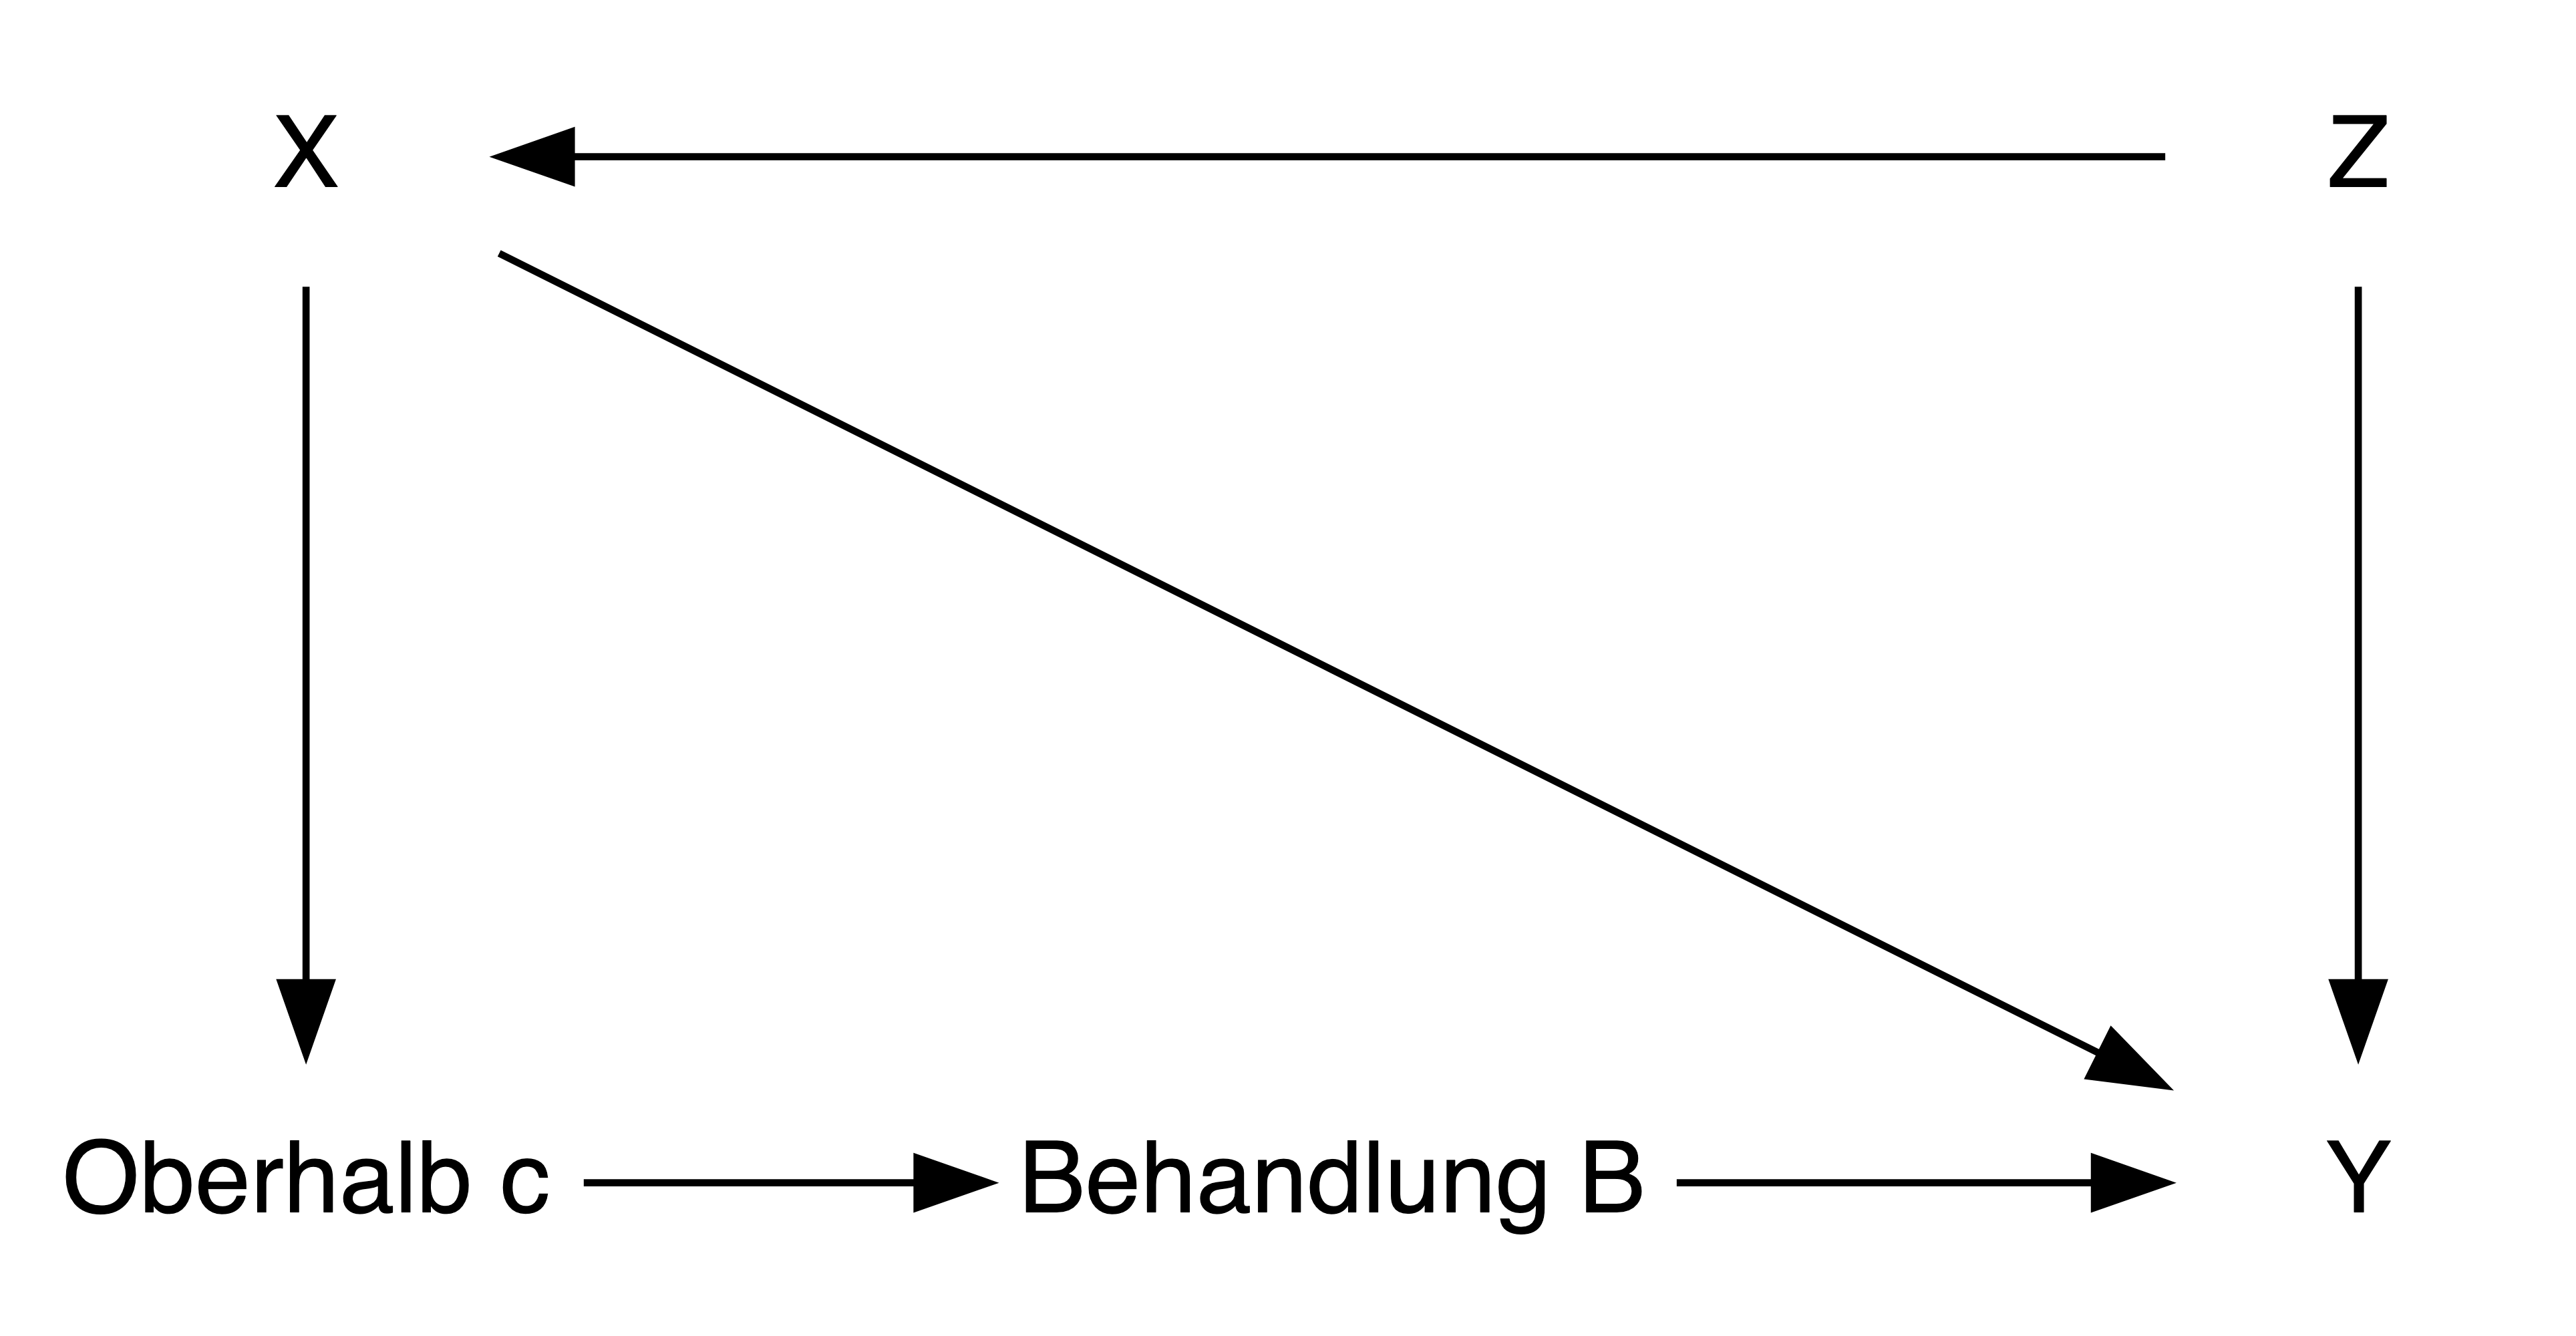
\includegraphics[width=5in,height=3in]{RDD_files/figure-latex/dot-figure-1.png}

}

\end{figure}

}

\caption{\label{fig-CDRDD}Kausales Diagramm für Sharp RDD}

\end{figure}

RDD isoliert Variation auf dem Pfad \emph{Oberhalb C → Behandlung B →
Y}. Somit können Backdoor-Pfade über \(X\) oder weitere (möglichweise
unbeobachtbare) Confounder (\(Z\)) vermieden werden, siehe
Abbildung~\ref{fig-CDRDD}. Der kausale Effekt wird dabei als (lokaler)
durchschnittlicher Behandlungseffekt der Diskontinuität auf die
Outcome-Variable (\(Y\)) anhand von Beobachtungen \emph{nahe bei c}
ermittelt.

Hinsichtlich der Beeinflussung der Behandlung unterscheiden wir zwischen
\emph{Sharp} und \emph{Fuzzy} Regression Discontinuity Designs
(SRDD/FRDD). Bei einem SRDD ist die Zuweisung der Behandlung
\emph{deterministisch}, d.h. der Schwellenwert in der Laufvariable ist
eine harte Grenze für die Gruppenzugehörigkeit: Die
\emph{Wahrscheinlichkeit} der Behandlung \(p\) springt bei \(X=c\) von
\(p=0\) um \(\Delta p = 1\) auf \(p=1\).

Bei einem FRDD ist die Zuordnung in Behandlungs- und Kontrollgruppe
nicht perfekt durch den Schwellenwert \(c\) bestimmt: Die
Behandlungswahrscheinlichkeit \(p\) springt bei \(X=c\) um
\(\Delta p<1\). Im FRDD können grundsätzlich also sowohl behandelte
Subjekte als auch Kontroll-Beobachtungen auf beiden Seiten der
Diskontinuität vorliegen -- die Trennung der Gruppen ist
``unscharf''\footnote{Engl. \emph{fuzzy}.}. Dieser Umstand ist oft in
empirischen Studien mit nicht-experimentellen Daten gegeben, wenn es
neben der Überschreitung von \(c\) weitere Determinanten der Behandlung
gibt (für die wir nicht kontrollieren können). Die Wahl zwischen SRDD
und FRDD hängt grundsätzlich vom datenerzeugenden Prozess und der
Forschungsfrage ab.

\hypertarget{sharp-regression-discontinuity-design}{%
\section{Sharp Regression Discontinuity
Design}\label{sharp-regression-discontinuity-design}}

\textbf{Modell und funktionale Form}

Die korrekte Spezifikation der funktionalen Form für ein RDD ist
wichtig, um eine verzerrte Schätzung des Effekts zu vermeiden. Die
einfachste Form eines SRDD kann anhand der linearen Regression
\begin{align}
Y_i = \beta_0 + \beta_1 B_i + \beta_2 X_i + u_i\label{eq-simpleSRDD}
\end{align} geschätzt werden, wobei \(B_i\) eine Dummy-Variable für das
Überschreiten des Schwellenwertes \(c\) ist, d.h. \begin{align*}
  B_i=\begin{cases}
    0 & X_i < c\\
    1 & X_i \geq c.
  \end{cases}
\end{align*} Damit ist \(B_i\) eine \emph{deterministische} Funktion der
Laufvariable \(X_i\) und zeigt die Zugehörigkeit zur Behandlungs- oder
Treatmentgruppe an. Der Koeffizient \(\beta_1\) misst den
Behandlungseffekt.

Das Modell \eqref{eq-simpleSRDD} unterstellt, dass \(X\) links- und
rechtsseitig von \(c\) denselben Effekt auf \(Y\) hat. Diese Annahme ist
restriktiv. Eine Alternative ist ein lineares Interaktionsmodell
\begin{align}
Y_i = \beta_0 + \beta_1 B_i + \beta_2 (X_i - c) + \beta_3(X_i - c)\times B_i + u_i.\label{eq:linearSRDD}
\end{align} Das Modell \eqref{eq:linearSRDD} kann unterschiedliche
lineare Effekte von \(X\) auf \(Y\) unterhalb (\(\beta_2\)) und oberhalb
(\(\beta_2 + \beta_3\)) von \(c\) abbilden. Beachte, dass \((X_i - c)\)
die um den Schwellenwert zentrierte Laufvariable ist, sodass \(\beta_1\)
wie in \eqref{eq-simpleSRDD} den Unterschied des Effekts von \(X\) auf
\(Y\) für Beoabachtungen am Schwellenwert erfasst.

Um unterschiedliche nicht-lineare Zusammenhänge von \(X\) und \(Y\)
unterhalb und oberhalb von \(c\) abzubilden, können (interargierte)
Polynom-Terme in \(X\) verwendet werden. Häufig wird eine quadratische
Regressionsfunktion genutzt, \begin{align}
  Y_i =&\, \beta_0 + \beta_1 B_i + \beta_2 (X_i - c) + \beta_3 (X_i - c)^2\\ 
       &+\, \beta_4(X_i - c)\times B_i + \beta_5(X_i - c)\times B_i + u_i.\label{eq:quadSRDD}
\end{align} Gelman und Imbens (2019) zeigen, dass Polynome höherer
Ordnung zu verzerrten Schätzern und hoher Varianz führen
können.\footnote{Ursachen sind Überanpassung an die Daten sowie
  instabiles Verhalten der Schätzung nahe des Schwellenwertes.} Die
Authoren empfehlen stattdessen die Schätzung mit lokaler Regression.

\textbf{Nicht-parametrische Schätzung und Bandweite}

Aktuelle Studien nutzen nicht-parametrische Schätzer, die den
Behandlungseffekt als Differenz der geschätzten Regressionsfunktionen am
Schwellenwert \(c\) berechnen. Um auch nicht-lineare
Regressionsfunktionen abzubilden zu können, wird häufig lokale
Regression verwendet. Dieses Verfahren liefert eine ``lokale'' Schätzung
der Regressionsfunktionen am Schwellenwert, bei der nur Beobachtungen
nahe \(X = c\) für die Schätzung berücksichtigt werden. Hinreichende
Nähe wird hierbei durch eine sogenannte Bandweite \(h\) festgelegt,
wobei \begin{align}
  \lvert(X_i-c)\rvert\leq h \label{eq:bwc}
\end{align} das Kriterium für eine Berücksichtigung von Beobachtung
\(i\) bei der Schätzung ist.

Unter Verwendung einer Bandweite \(h\) wird der Regressionsansatz
\eqref{eq:linearSRDD} als \emph{lokale lineare Regression} mit
Uniform-Kernelfunktion bezeichnet. Der Uniform-Kernel gibt allen
Beobachtungen, innerhalb der Bandweite \(h\) dasselbe Gewicht. Ist \(h\)
so groß, dass der gesamte Datensatz in die Schätzung einbezogen wird,
entspricht der lokale lineare Regressions-Schätzer mit Uniform-Kernel
dem (globalen) KQ-Schätzer in einem linearen Interaktionsmodell anhand
aller Beobachtungen. Neben dem Uniform-Kernel ist der Triangular-Kernel
eine in der Praxis häufig genutzte lineare Kernelfunktion. Der
nachstehende Code plottet die Uniform- (grün) sowie die
Triangular-Kernelfunktion (blau), siehe Abbildung~\ref{fig-linearkern}.

\begin{Shaded}
\begin{Highlighting}[]
\FunctionTok{library}\NormalTok{(ggplot2)}
\FunctionTok{library}\NormalTok{(cowplot)}

\CommentTok{\# Kernelfunktionen zeichnen}
\FunctionTok{ggplot}\NormalTok{() }\SpecialCharTok{+} 
    \FunctionTok{geom\_function}\NormalTok{(}
      \AttributeTok{fun =} \SpecialCharTok{\textasciitilde{}} \FunctionTok{ifelse}\NormalTok{(}
        \AttributeTok{test =} \FunctionTok{abs}\NormalTok{(.) }\SpecialCharTok{\textless{}=} \DecValTok{1}\NormalTok{,}
        \AttributeTok{yes =}  \DecValTok{1}\SpecialCharTok{/}\DecValTok{2}\NormalTok{, }
        \AttributeTok{no =} \DecValTok{0}
\NormalTok{      ), }
      \AttributeTok{col =} \StringTok{"green"}\NormalTok{, }
      \AttributeTok{n =} \DecValTok{1000}
\NormalTok{      ) }\SpecialCharTok{+} 
    \FunctionTok{geom\_function}\NormalTok{(}
      \AttributeTok{fun =} \SpecialCharTok{\textasciitilde{}} \FunctionTok{ifelse}\NormalTok{(}
        \AttributeTok{test =} \FunctionTok{abs}\NormalTok{(.) }\SpecialCharTok{\textless{}=} \DecValTok{1}\NormalTok{, }
        \AttributeTok{yes =} \DecValTok{1} \SpecialCharTok{{-}} \FunctionTok{abs}\NormalTok{(.), }
        \AttributeTok{no =} \DecValTok{0}
\NormalTok{      ), }
      \AttributeTok{col =} \StringTok{"blue"}\NormalTok{, }
      \AttributeTok{n =} \DecValTok{100}
\NormalTok{      ) }\SpecialCharTok{+} 
    \FunctionTok{scale\_x\_continuous}\NormalTok{(}
      \AttributeTok{name =} \StringTok{"x"}\NormalTok{, }
      \AttributeTok{limits =} \FunctionTok{c}\NormalTok{(}\SpecialCharTok{{-}}\FloatTok{1.5}\NormalTok{, }\FloatTok{1.5}\NormalTok{), }
      \AttributeTok{breaks =} \FunctionTok{c}\NormalTok{(}\SpecialCharTok{{-}}\DecValTok{1}\NormalTok{, }\DecValTok{0}\NormalTok{, }\DecValTok{1}\NormalTok{)}
\NormalTok{    ) }\SpecialCharTok{+}
    \FunctionTok{scale\_y\_continuous}\NormalTok{(}
      \AttributeTok{name =} \StringTok{"K(x)"}\NormalTok{, }
      \AttributeTok{breaks =} \FunctionTok{c}\NormalTok{(}\DecValTok{0}\NormalTok{, }\DecValTok{1}\NormalTok{), }
      \AttributeTok{limits =} \FunctionTok{c}\NormalTok{(}\DecValTok{0}\NormalTok{, }\FloatTok{1.25}\NormalTok{)}
\NormalTok{    ) }\SpecialCharTok{+}
    \FunctionTok{theme\_cowplot}\NormalTok{()}
\end{Highlighting}
\end{Shaded}

\begin{figure}[t]

{\centering 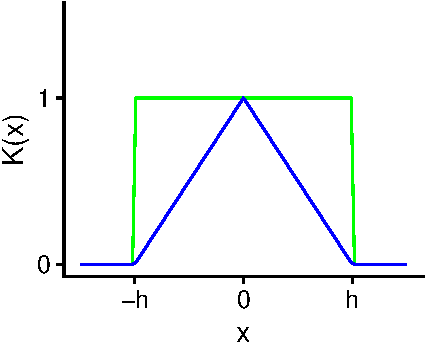
\includegraphics{RDD_files/figure-pdf/fig-linearkern-1.pdf}

}

\caption{\label{fig-linearkern}Kernelfunktionen auf {[}-1, 1{]}}

\end{figure}

In empirischen Studien wird als Basis-Spezifikation oft eine lokale
lineare Regression anhand von \eqref{eq:linearSRDD} mit einer linearen
Kernelfunktionen und geringer bandweite \(h\) genutzt. Anschließend wird
die Robustheit der Ergebnisse anhand flexiblerer Spezifikationen, die
Nicht-Linearitäten in der Regressionsfunktion besser abbilden können,
geprüft.

Die nachstehende Visualisierung zeigt die Schätzung des kausalen
Effektes der Behandlung \(B_i\) anhand lokaler linearer Regression mit
einem Uniform-Kernel für wiefolgt simulierte Daten: \begin{align*}
  Y_i =&\, \beta_1 X_i + \beta_2 B + \beta_3 X_i^2 \times B_i + u_i,\\
  \\
  u_i \sim&\, N(0, 0.5), \quad X_i \sim U(0, 10), \quad B = \mathbb{I}(X_i \geq c = 5)\\
  \beta_1 =&\, .5, \quad \beta_2 = 1.5, \quad \beta_3 = -0.15
\end{align*}

Diese Vorschrift ist schnell mit R umgesetzt:

\begin{Shaded}
\begin{Highlighting}[]
\FunctionTok{set.seed}\NormalTok{(}\DecValTok{1234}\NormalTok{)}
\CommentTok{\# Anz.Beobachtungen}
\NormalTok{n }\OtherTok{\textless{}{-}} \DecValTok{750}

\CommentTok{\# Parameter definieren}
\NormalTok{c }\OtherTok{\textless{}{-}} \DecValTok{5}
\NormalTok{beta\_1 }\OtherTok{\textless{}{-}}\NormalTok{ .}\DecValTok{5}
\NormalTok{beta\_2 }\OtherTok{\textless{}{-}} \FloatTok{1.5}
\NormalTok{beta\_3 }\OtherTok{\textless{}{-}} \SpecialCharTok{{-}}\NormalTok{.}\DecValTok{15}

\CommentTok{\# Regressionsfunktion definieren}
\NormalTok{f }\OtherTok{\textless{}{-}} \ControlFlowTok{function}\NormalTok{(X) \{}
\NormalTok{  beta\_1 }\SpecialCharTok{*}\NormalTok{ (X }\SpecialCharTok{{-}}\NormalTok{ c) }\SpecialCharTok{+}\NormalTok{ beta\_2 }\SpecialCharTok{*}\NormalTok{ B }\SpecialCharTok{+}\NormalTok{ beta\_3 }\SpecialCharTok{*}\NormalTok{ B }\SpecialCharTok{*}\NormalTok{ (X }\SpecialCharTok{{-}}\NormalTok{ c)}\SpecialCharTok{\^{}}\DecValTok{2}
\NormalTok{\}}

\CommentTok{\# Daten erzeugen}
\NormalTok{X }\OtherTok{\textless{}{-}} \FunctionTok{runif}\NormalTok{(n, }\DecValTok{0}\NormalTok{, }\DecValTok{11}\NormalTok{)}
\NormalTok{B }\OtherTok{\textless{}{-}} \FunctionTok{ifelse}\NormalTok{(X }\SpecialCharTok{{-}}\NormalTok{ c }\SpecialCharTok{\textgreater{}=} \DecValTok{0}\NormalTok{, }\DecValTok{1}\NormalTok{, }\DecValTok{0}\NormalTok{)}
\NormalTok{Y }\OtherTok{\textless{}{-}} \FunctionTok{f}\NormalTok{(X) }\SpecialCharTok{+} \FunctionTok{rnorm}\NormalTok{(n, }\AttributeTok{sd =}\NormalTok{ .}\DecValTok{5}\NormalTok{)}

\CommentTok{\# Beoabchtungen sammeln}
\NormalTok{dat }\OtherTok{\textless{}{-}} \FunctionTok{data.frame}\NormalTok{(}
  \AttributeTok{Y =}\NormalTok{ Y, }\AttributeTok{X =}\NormalTok{ X }\SpecialCharTok{{-}}\NormalTok{ c, }\AttributeTok{B =}\NormalTok{ B}
\NormalTok{)}
\end{Highlighting}
\end{Shaded}

\begin{center}\rule{0.5\linewidth}{0.5pt}\end{center}

\textbf{\emph{Diese interaktive Komponente des Buchs ist nur in der
Online-Version verfügbar}}

\begin{center}\rule{0.5\linewidth}{0.5pt}\end{center}

Der interssierende Effekt am Schwellenwert \(c=5\) beträgt
\(\beta_2 = 1.5\). Beachte, dass aufgrund des Terms
\(\beta_3 X_i^2 \times B_i\) ein quadratischer Zusammenhang von \(Y\)
und \(X\) oberhalb von \(X_i = c\) vorliegt. Es können folgende
Eigenschaften der Schätzung in Abhängigkeit von der Bandweite \(h\)
beobachtet werden:

\begin{itemize}
\item
  Für die voreingestellte Bandweite \(h = 1.3\) liefert die lokale
  lineare Regression eine gute Approximation des
  Regressionszusammenhangs auf beiden Seiten des Schwellenwertes und die
  Schätzung des Behandlungseffekts liegt nahe beim wahren Wert
  \(\beta_2 = 1.5\).
\item
  Für kleinere Bandweiten verringert sich die Datenbasis der Schätzung.
  Die Varianz der Schätzung nimmt zu und die Approximation der
  Regressionsfunktion verschlechtert sich. Wir beobachten eine mit
  \(h\to0\) zunehmende Verzerrung bei der Schätzung des
  Behandlungseffekts.
\item
  Größere Bandweiten \(h\) erhöhen die Datenbasis der Schätzung, führen
  aber zu einer Annäherung der lokalen Schätzung an die globale
  KQ-Schätzung. Linksseitig des Schwellenwertes erzielen wir damit eine
  Schätzung mit hoher Güte. Rechsseitig von \(X_i = c\) verschlechtert
  sich die lokale Anpassung am Schwellenwert deutlich, weil die lineare
  Schätzung den tatsächlichen (nicht-linearen) Zusammenhang nicht
  adäquat abbilden kann. Die Schätzung des Behandlungseffekts ist hier
  deutlich verzerrt.
\end{itemize}

Die Wahl der Bandweite ist also eine wichtige Komponenten der
RDD-Schätzung: Kleine Bandweiten erlauben eine Schätzung der
Regressionsfunktion nahe des Schwellenwertes mit wenig Verzerrung.
Allerdings kann diese Schätzung unpräzise sein, wenn nur wenige
Beobachtungen \eqref{eq:bwc} erfüllen. In der Praxis wird \(h\) daher
mit einem analytischen Schätzer (vgl. G. Imbens und Kalyanaraman 2012)
oder anhand von \emph{Cross Validation} (bspw. G. W. Imbens und Lemieux
2008) bestimmt. Die später in diesem Kapitel betrachteten R-Pakete
halten diese Methoden bereit.

\hypertarget{manipulation-am-schwellenwert}{%
\section{Manipulation am
Schwellenwert}\label{manipulation-am-schwellenwert}}

Eine wichtige Annahmen für die Gültigkeit einer RDD-Schätzung ist, dass
keine Manipulation der Gruppenzugehörigkeit am Schwellenwert vorliegt.
Wenn sich Subjekte nahe des Schwellenwertes \(c\) --- d.h. in
Abhängigkeit der Laufvariable \(X\) --- systematisch in den Confoundern
\(Z\) unterscheiden, können wir den Backdoor-Pfad \emph{Oberhalb C →
Behandlung B → Y} nicht isolieren. Wir erhalten dann eine verzerrte
Schätzung des Behandlungseffekts.

In empirischen Studien mit Individuen kann Selbstselektion auftreten:
Menschen mit \(X<c\) aber nahe \(c\) (hier Kontrollgruppe) könnten
aufgrund unbeobachtbarer Eigenschaften \(Z\) die Ausprägung ihrer
Laufvariable zu \(X>c\) (hier Behandlungsgruppe) manipulieren. Wenn
\(Z\) die Outcome-Variable beeinflusst, bleibt der Backdoor-Pfad
\emph{Oberhalb C → Behandlung B → Y} so bestehen.

Manipulation resultiert in Häufung von Beobachtungen am Schwellenwert.
Dei Verteilung der Laufvariable kann auf diese Unregelmäßigkeit hin
untersucht werden. McCrary (2008) schlägt hierfür einen Verfahren vor,
das die Kontinuität der Dichtefunktion von \(X\) am Schwellenwert
testet.

Der Test von McCrary (2008) ist in \texttt{rdd::DCdensity()}
implementiert. Wir zeigen die Anwendung des Tests anhand der oben
simulierten Daten. Beachte, dass \(X_i\sim U(0, 10)\), d.h. die
Laufvariable ist bei \(X_i = c\) kontinuierlich verteilt. Die
Nullhypothese (keine Manipulation) gilt für die simulierten Daten

\begin{Shaded}
\begin{Highlighting}[]
\CommentTok{\# McCrary{-}Test durchführen}
\NormalTok{p\_mccrary }\OtherTok{\textless{}{-}}\NormalTok{ rdd}\SpecialCharTok{::}\FunctionTok{DCdensity}\NormalTok{(}
  \AttributeTok{runvar =}\NormalTok{ X, }
  \AttributeTok{cutpoint =}\NormalTok{ c, }
  \AttributeTok{plot =}\NormalTok{ F}
\NormalTok{)}

\CommentTok{\# p{-}Wert}
\NormalTok{p\_mccrary}
\end{Highlighting}
\end{Shaded}

\begin{verbatim}
[1] 0.5013939
\end{verbatim}

Der p-Wert 0.5 ist größer als jedes übliche Signifikanzniveau. Damit
liegt starke Evidenz für die Nullhypothese (keine Diskontinuität) und
gegen Manipulation am Schwellenwert vor.

Cattaneo, Jansson, und Ma (2020) (CMJ) schlagen eine Weiterentwicklung
des McCrary-Tests vor, die höhere statistische Macht gegenüber
Diskontinuitäten hat am Schwellenwert hat. Der CJM-Test ist im Paket
\texttt{rddensity} implementiert.

\begin{Shaded}
\begin{Highlighting}[]
\FunctionTok{library}\NormalTok{(rddensity)}

\CommentTok{\# CJM Schätzer berechnen}
\NormalTok{CJM }\OtherTok{\textless{}{-}} \FunctionTok{rddensity}\NormalTok{(X, }\AttributeTok{c =} \DecValTok{5}\NormalTok{)}
\end{Highlighting}
\end{Shaded}

Mit der Funktion \texttt{rddensity::rdplotdensity()} erzeugen wir
Abbildung~\ref{fig-cjmtsim}.

\begin{Shaded}
\begin{Highlighting}[]
\CommentTok{\# Plot für Dichtefunktion erstellen}
\NormalTok{plot }\OtherTok{\textless{}{-}} \FunctionTok{rdplotdensity}\NormalTok{(}
  \AttributeTok{rdd =}\NormalTok{ CJM, }
  \AttributeTok{X =}\NormalTok{ X, }
  \CommentTok{\# für Punkte{-} und Linienplots:}
  \AttributeTok{type =} \StringTok{"both"} 
\NormalTok{)}
\end{Highlighting}
\end{Shaded}

\begin{figure}[t]

{\centering 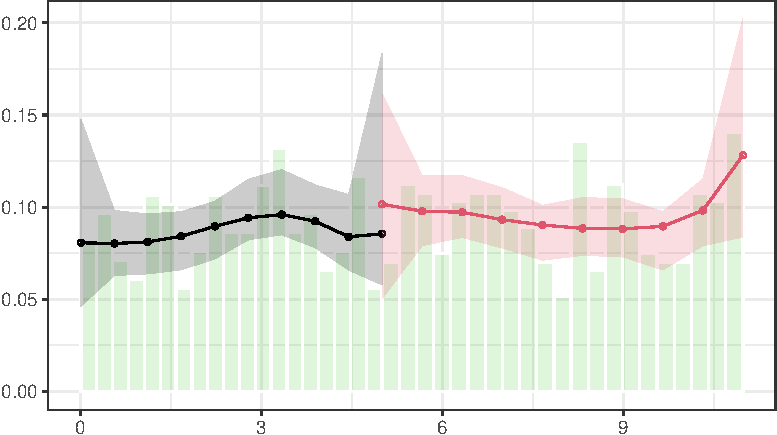
\includegraphics{RDD_files/figure-pdf/fig-cjmtsim-1.pdf}

}

\caption{\label{fig-cjmtsim}CJM-Test -- geschätzte Dichtefunktionen der
Laufvariable auf beiden Seiten des Schwellenwerts c = 5}

\end{figure}

Abbildung~\ref{fig-cjmtsim} zeigt die geschätzten Dichtefunktionen.
Erwartungsgemäß finden wir eine große Überlappung der zugehörigen
Konfidenzbänder (schattierte Flächen) am Schwellenwert \(c=5\).

Mit \texttt{summary()} erhalten wir eine detaillierte Zusammenfassung
des Tests.

\begin{Shaded}
\begin{Highlighting}[]
\CommentTok{\# Statistische Zusammenfassung des CJM{-}Tests}
\FunctionTok{summary}\NormalTok{(CJM)}
\end{Highlighting}
\end{Shaded}

\begin{verbatim}

Manipulation testing using local polynomial density estimation.

Number of obs =       750
Model =               unrestricted
Kernel =              triangular
BW method =           estimated
VCE method =          jackknife

c = 5                 Left of c           Right of c          
Number of obs         329                 421                 
Eff. Number of obs    133                 154                 
Order est. (p)        2                   2                   
Order bias (q)        3                   3                   
BW est. (h)           1.918               2.124               

Method                T                   P > |T|             
Robust                -0.3338             0.7385              


P-values of binomial tests (H0: p=0.5).

Window Length              <c     >=c    P>|T|
0.346     + 0.346          20      21    1.0000
0.521     + 0.544          34      37    0.8126
0.696     + 0.742          44      57    0.2323
0.870     + 0.939          54      64    0.4075
1.045     + 1.137          62      77    0.2349
1.220     + 1.334          73      98    0.0661
1.394     + 1.532          86     106    0.1701
1.569     + 1.729          96     124    0.0685
1.743     + 1.927         119     140    0.2139
1.918     + 2.124         133     154    0.2377
\end{verbatim}

Gemäß des p-Werts (\texttt{P\ \textgreater{}\ \textbar{}T\textbar{}})
von 0.74 spricht der CJM-Test noch deutlicher gegen eine Diskontinuität
als der McCrary-Test.

\hypertarget{case-study-amtsinhaber-vorteil-lee2008}{%
\subsection{Case Study: Amtsinhaber-Vorteil (Lee
2008)}\label{case-study-amtsinhaber-vorteil-lee2008}}

Lee (2008) untersucht den Einfluss des Amtsinhaber-Vorteils auf die Wahl
von Mitgliedern des US-Repräsentantenhaus. In den meisten Wahlkreisen
entfallen große Anteile der Stimmen (oder gar ausschließlich) auf
demokratische und republikanische Kanditat*innen, sodass sich die Studie
auf diese Parteien beschränkt. Entfällt die Mehrheit der Stimmen auf
eine*n Kandiat*in, gewinnt diese*r den Sitz für den Wahlkreis. Durch die
Analyse der 6558 Wahlen im Zeitraum 1946-1998 mit einem SRDD kommt die
Studie zu dem Ergebnis, dass Amtsinhabende im Durchschnitt einen Vorteil
von etwa 8\% bis 10\% bei der Wahl haben. Dieses Ergebnis kann
verschiedene Ursachen haben, bspw. dass die amtierende Partei höhere
finanzielle Ressourcen besitzt und von einer besseren Organisation und
durch Instrumenalisierung staatlicher Strukturen für die eigenen Zwecke
profitiert.

Anhand der Datensätze \texttt{house} und \texttt{house\_binned}
illustrieren wir nachfolgend die Schätzung von SRDD-Modellen für den
Wahlerfolg der demokratischen Partei, wenn diese Amtsinhaber ist. Wir
lesen hierfür zunächst die Datensätze \texttt{house} und
\texttt{house\_binned} ein und verschaffen uns einen Überblick.

\begin{Shaded}
\begin{Highlighting}[]
\FunctionTok{library}\NormalTok{(tidyverse)}
\FunctionTok{library}\NormalTok{(modelsummary)}

\CommentTok{\# Daten einlesen}
\NormalTok{house }\OtherTok{\textless{}{-}} \FunctionTok{read\_csv}\NormalTok{(}\StringTok{"datasets/house.csv"}\NormalTok{)}
\CommentTok{\# Gruppierter Datensatz}
\NormalTok{house\_binned }\OtherTok{\textless{}{-}} \FunctionTok{read\_csv}\NormalTok{(}\StringTok{"datasets/house\_binned.csv"}\NormalTok{)}

\CommentTok{\# Überblick verschaffen}
\FunctionTok{glimpse}\NormalTok{(house)}
\end{Highlighting}
\end{Shaded}

\begin{verbatim}
Rows: 6,558
Columns: 2
$ StimmenTm1 <dbl> 0.1049, 0.1393, -0.0736, 0.0868, 0.3994, 0.1681, 0.2516, 0.~
$ StimmenT   <dbl> 0.5810, 0.4611, 0.5434, 0.5846, 0.5803, 0.6244, 0.4873, 0.5~
\end{verbatim}

\begin{Shaded}
\begin{Highlighting}[]
\FunctionTok{glimpse}\NormalTok{(house\_binned)}
\end{Highlighting}
\end{Shaded}

\begin{verbatim}
Rows: 100
Columns: 2
$ StimmenT   <dbl> 0.5995600, 0.5657000, 0.4272554, 0.5637456, 0.6868627, 0.60~
$ StimmenTm1 <dbl> 0.104764444, 0.135005263, -0.075690769, 0.084570886, 0.3951~
\end{verbatim}

Der Datensatz \texttt{house} enthält die Stimmenanteile demokratischer
Kandidat*innen bei der Wahl zum Zeitpunkt \(T\) (\(StimmenT\)) sowie die
Differenz zwischen demokratischen und republikanischen Stimmenanteilen
bei der vorherigen Wahl, d.h. zum Zeitpunkt \(T-1\) (\(StimmenTm1\)).
Der Schwellenwert für einen Wahlsieg liegt bei Stimmengleichheit, d.h.
\(StimmenTm1 = 0\).

\texttt{house\_binned} ist eine aggregierte Version von \texttt{house}
mit Mittelwerten von jeweils 50 gleichgroßen Intervallen oberhalb und
unterhalb der Schwelle von \(StimmenTm1 = 0\). Dieser Datensatz eignet
sich, um einen ersten Eindruck des funktionalen Zusammenhangs auf beiden
Seiten zu erhalten. Wir stellen zunächst diese klassierten Daten mit
\texttt{ggplot2} graphisch dar.

\begin{Shaded}
\begin{Highlighting}[]
\CommentTok{\# Klassierte Daten plotten}
\NormalTok{house\_binned }\SpecialCharTok{\%\textgreater{}\%}
  \FunctionTok{ggplot}\NormalTok{(}
    \FunctionTok{aes}\NormalTok{(}\AttributeTok{x =}\NormalTok{ StimmenTm1, }\AttributeTok{y =}\NormalTok{ StimmenT)}
\NormalTok{    ) }\SpecialCharTok{+}
  \FunctionTok{geom\_point}\NormalTok{() }\SpecialCharTok{+}
  \FunctionTok{geom\_vline}\NormalTok{(}\AttributeTok{xintercept =} \DecValTok{0}\NormalTok{, }\AttributeTok{lty =} \DecValTok{2}\NormalTok{)}
\end{Highlighting}
\end{Shaded}

\begin{figure}[t]

{\centering 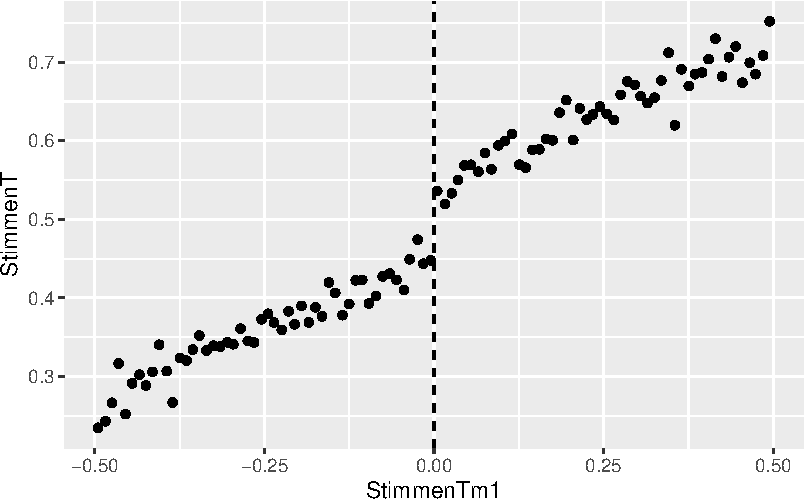
\includegraphics{RDD_files/figure-pdf/fig-LeeDataClass-1.pdf}

}

\caption{\label{fig-LeeDataClass}Klassierte Daten aus Lee (2008)}

\end{figure}

Die Grafik zeigt eindeutig einen Sprung von \(StimmenT\) bei
\(StimmenTm1 = 0\). Weiterhin erkennen wir, dass der Zusammenhang nahe
\(0\) vermutlich jeweils gut durch eine lineare Funktion approximiert
werden kann. Eine Modell-Spezifikation mit gleicher Steigung auf beiden
Seiten des Schwellenwertes scheint hingegen weniger gut geeignet. Wir
vergleichen diese Spezifikationen nachfolgend.

Zunächst fügen wir dem Datensatz eine Dummyvariable \texttt{B} hinzu.
Diese dient als Indikator für den Wahlgewinn in der letzten Wahl und
zeigt die Amtsinhaberschaft (Behandlung) an.

\begin{Shaded}
\begin{Highlighting}[]
\CommentTok{\# Behandlungsindikator B hinzufügen}
\NormalTok{house }\OtherTok{\textless{}{-}}\NormalTok{ house }\SpecialCharTok{\%\textgreater{}\%} 
  \FunctionTok{mutate}\NormalTok{(}\AttributeTok{B =}\NormalTok{ StimmenTm1 }\SpecialCharTok{\textgreater{}} \DecValTok{0}\NormalTok{)}

\FunctionTok{glimpse}\NormalTok{(house)}
\end{Highlighting}
\end{Shaded}

\begin{verbatim}
Rows: 6,558
Columns: 3
$ StimmenTm1 <dbl> 0.1049, 0.1393, -0.0736, 0.0868, 0.3994, 0.1681, 0.2516, 0.~
$ StimmenT   <dbl> 0.5810, 0.4611, 0.5434, 0.5846, 0.5803, 0.6244, 0.4873, 0.5~
$ B          <lgl> TRUE, TRUE, FALSE, TRUE, TRUE, TRUE, TRUE, TRUE, TRUE, TRUE~
\end{verbatim}

Wir überprüfen die Laufvariable mit dem CJM-Test auf Manipulation am
Schwellenwert \(c=0\).

\begin{Shaded}
\begin{Highlighting}[]
\CommentTok{\# CJM{-}Test durchführen}
\NormalTok{CJM\_Lee }\OtherTok{\textless{}{-}} \FunctionTok{rddensity}\NormalTok{(}\AttributeTok{X =}\NormalTok{ house}\SpecialCharTok{$}\NormalTok{StimmenTm1)}

\CommentTok{\# Zusammenfassung anzeigen}
\FunctionTok{summary}\NormalTok{(CJM\_Lee)}
\end{Highlighting}
\end{Shaded}

\begin{verbatim}

Manipulation testing using local polynomial density estimation.

Number of obs =       6558
Model =               unrestricted
Kernel =              triangular
BW method =           estimated
VCE method =          jackknife

c = 0                 Left of c           Right of c          
Number of obs         2740                3818                
Eff. Number of obs    1297                1360                
Order est. (p)        2                   2                   
Order bias (q)        3                   3                   
BW est. (h)           0.236               0.243               

Method                T                   P > |T|             
Robust                1.4346              0.1514              


P-values of binomial tests (H0: p=0.5).

Window Length / 2          <c     >=c    P>|T|
0.004                      21      24    0.7660
0.007                      38      46    0.4452
0.011                      50      60    0.3909
0.014                      73      77    0.8066
0.018                      91     104    0.3902
0.022                     124     132    0.6618
0.025                     149     149    1.0000
0.029                     163     174    0.5860
0.032                     176     202    0.1984
0.036                     197     223    0.2225
\end{verbatim}

\begin{Shaded}
\begin{Highlighting}[]
\CommentTok{\# CJM{-}Plot}
\NormalTok{plot }\OtherTok{\textless{}{-}} \FunctionTok{rdplotdensity}\NormalTok{(}
  \AttributeTok{rdd =}\NormalTok{ CJM\_Lee,}
  \AttributeTok{X =}\NormalTok{ house}\SpecialCharTok{$}\NormalTok{StimmenTm1, }
  \AttributeTok{type =} \StringTok{"both"}\NormalTok{, }
\NormalTok{)}
\end{Highlighting}
\end{Shaded}

\begin{figure}[t]

{\centering 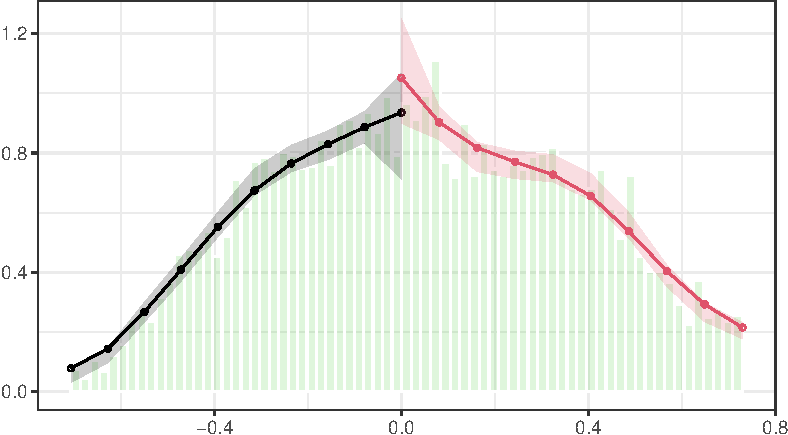
\includegraphics{RDD_files/figure-pdf/fig-cjm-lee-1.pdf}

}

\caption{\label{fig-cjm-lee}CJM-Test -- geschätzte Dichtefunktionen der
Laufvariable}

\end{figure}

Abbildung~\ref{fig-cjm-lee} und der p-Wert von \(0.15\) sind Evidenz
gegen eine Manipulation am Schwellenwert.

Um den Behandlungseffekt anhand eines SRDDs zu ermitteln, schätzen wir
das Interaktionsmodell \begin{align*}
  \text{StimmenT}_i =&\, \beta_0 + \beta_1 B_i + \beta_2 (\text{StimmenTm1}_i - 50)\\ 
  +&\, \beta_3(\text{StimmenTm1}_i - 50)\times B_i + u_i
\end{align*} zunächst für eine Bandweite von \(h = 0.5\). Aufgrund der
Skalierung der Daten (Wahlergebnisse in \%) bedeutet dies die Verwendung
des \emph{gesamten} Datensatzes für die Schätzung.

\begin{Shaded}
\begin{Highlighting}[]
\CommentTok{\# Interaktionsmodell schätzen}
\NormalTok{house\_llr1 }\OtherTok{\textless{}{-}} \FunctionTok{lm}\NormalTok{(}
  \AttributeTok{formula =}\NormalTok{ StimmenT }\SpecialCharTok{\textasciitilde{}}\NormalTok{ B }\SpecialCharTok{*}\NormalTok{ StimmenTm1, }
  \AttributeTok{data =}\NormalTok{ house}
\NormalTok{)}

\CommentTok{\# Zusammenfassung anzeigen  }
\FunctionTok{modelsummary}\NormalTok{(}
  \AttributeTok{models =}\NormalTok{ house\_llr1, }
  \AttributeTok{vcov =} \StringTok{"HC1"}\NormalTok{, }\CommentTok{\# robuste Standardfehler}
  \AttributeTok{stars =}\NormalTok{ T, }
  \AttributeTok{gof\_map =} \StringTok{"nobs"}\NormalTok{, }
  \AttributeTok{output =} \StringTok{"gt"}
\NormalTok{) }\SpecialCharTok{\%\textgreater{}\%} 
\NormalTok{  tabopts}
\end{Highlighting}
\end{Shaded}

\setlength{\LTpost}{0mm}
\begin{longtable*}{lc}
\toprule
  & (1) \\ 
\midrule\addlinespace[2.5pt]
(Intercept) & 0.433*** \\ 
 & (0.004) \\ 
BTRUE & 0.118*** \\ 
 & (0.006) \\ 
StimmenTm1 & 0.297*** \\ 
 & (0.016) \\ 
BTRUE × StimmenTm1 & 0.046* \\ 
 & (0.018) \\ 
Num.Obs. & 6558 \\ 
\bottomrule
\end{longtable*}
\begin{minipage}{\linewidth}
+ p < 0.1, * p < 0.05, ** p < 0.01, *** p < 0.001\\
\end{minipage}

Der geschätzte Koeffizient von \(B\) (\texttt{BTRUE}) beträgt etwa
\(0.12\) und ist hochsignifikant. Übereinstimmend mit
Abbildung~\ref{fig-LeeDataClass} erhalten wir also eine positive
Schätzung des Behandlungseffekts. Die Interpretation ist, dass die
amtierenden Demokraten bei der Wahl von einem Amtsinhabervorteil
profitieren. Dieser Effekt schlägt sich als Stimmenbonus von geschätzten
12\% nieder. Diese Schätzung des Behandlungseffekts könnte jedoch
verzerrt sein:

\begin{itemize}
\item
  Die (implizite) Wahl von \(h=0.5\) in unserer Schätzung macht die
  Isolation des relevanten Frontdoor-Paths (\(c=0\) → Treatment →
  StimmenT) wenig plausibel. \(h\) sollte mit einer datengetriebenen
  Methode gewählt werden.
\item
  Weiterhin könnte die lineare funktionale Form der Regression inadäquat
  sein: Die lineare Approximation der wahren Regressionsfunktion nahe
  des Schwellenwerts \(0\) könnte unzureichend sein und in einer
  verzerrten Schätzung des Effekts resultieren. Zur Überprüfung der
  Robustheit der Ergebnisse sollte mit Schätzungen anhand nicht-linearer
  Spezifikationen verglichen werden.
\end{itemize}

Um diesen Gefahren für die Validität der Studie zu begegnen, schätzen
wir nun weitere Spezifikationen. Im Folgenden verwenden wir eine
Bandweitenschätzung gemäß G. Imbens und Kalyanaraman (2012).

\begin{Shaded}
\begin{Highlighting}[]
\CommentTok{\# Bandweite mit Schätzer von IK (2012) berechnen}
\NormalTok{(}
\NormalTok{IK\_BW }\OtherTok{\textless{}{-}} 
\NormalTok{  rdd}\SpecialCharTok{::}\FunctionTok{IKbandwidth}\NormalTok{(}
    \AttributeTok{X =}\NormalTok{ house}\SpecialCharTok{$}\NormalTok{StimmenTm1, }
    \AttributeTok{Y =}\NormalTok{ house}\SpecialCharTok{$}\NormalTok{StimmenT}
\NormalTok{  )}
\NormalTok{)}
\end{Highlighting}
\end{Shaded}

\begin{verbatim}
[1] 0.2685123
\end{verbatim}

Wir schätzen zunächst erneut das lineare Interaktionsmodell, diesmal
jedoch mit der Bandweite \texttt{IK\_BW}.

\begin{Shaded}
\begin{Highlighting}[]
\CommentTok{\# Lineares Interaktionsmodelle mit IK{-}Bandweite}
\NormalTok{house\_llin\_IK }\OtherTok{\textless{}{-}} \FunctionTok{lm}\NormalTok{(}
  \AttributeTok{formula =}\NormalTok{ StimmenT }\SpecialCharTok{\textasciitilde{}}\NormalTok{ B }\SpecialCharTok{*}\NormalTok{ StimmenTm1, }
  \AttributeTok{data =}\NormalTok{ house }\SpecialCharTok{\%\textgreater{}\%} 
    \FunctionTok{filter}\NormalTok{(}
      \FunctionTok{abs}\NormalTok{(StimmenTm1) }\SpecialCharTok{\textless{}=}\NormalTok{ IK\_BW}
\NormalTok{    )}
\NormalTok{)}
\end{Highlighting}
\end{Shaded}

Für den Vergleich mit einer nicht-linearen Spezifikation schätzen wir
auch ein quadratisches Interaktionsmodell.

\begin{Shaded}
\begin{Highlighting}[]
\CommentTok{\# Quadratisches Interaktionsmodell mit IK{-}Bandweite}
\NormalTok{house\_poly\_IK }\OtherTok{\textless{}{-}} \FunctionTok{update}\NormalTok{(}
  \AttributeTok{object =}\NormalTok{ house\_llin\_IK,}
  \AttributeTok{formula =}\NormalTok{ StimmenT }\SpecialCharTok{\textasciitilde{}}\NormalTok{ B }\SpecialCharTok{*} \FunctionTok{poly}\NormalTok{(StimmenTm1, }\AttributeTok{degree =} \DecValTok{2}\NormalTok{, }\AttributeTok{raw =}\NormalTok{ T)}
\NormalTok{)}
\end{Highlighting}
\end{Shaded}

Für eine Gegenüberstellung der Ergebnisse verwenden wir
\texttt{modelsummary()}.

\begin{Shaded}
\begin{Highlighting}[]
\CommentTok{\# Tabellarischer Modellvergleich}
\FunctionTok{modelsummary}\NormalTok{(}
  \AttributeTok{models =} \FunctionTok{list}\NormalTok{(}
    \StringTok{"Linear int."} \OtherTok{=}\NormalTok{ house\_llin\_IK, }
    \StringTok{"Quadratisch int."} \OtherTok{=}\NormalTok{ house\_poly\_IK}
\NormalTok{  ),  }
  \AttributeTok{vcov =} \StringTok{"HC1"}\NormalTok{, }
  \AttributeTok{stars =}\NormalTok{ T,}
  \AttributeTok{gof\_map =} \StringTok{"nobs"}\NormalTok{, }
  \AttributeTok{output =} \StringTok{"gt"}
\NormalTok{) }\SpecialCharTok{\%\textgreater{}\%} 
\NormalTok{  tabopts}
\end{Highlighting}
\end{Shaded}

\hypertarget{tbl-intmodsLee}{}
\setlength{\LTpost}{0mm}
\begin{longtable}{lcc}
\caption{\label{tbl-intmodsLee}Vergleich von SRDD-Interaktionsmodellen für Lee (2008) }\tabularnewline

\toprule
  & Linear int. & Quadratisch int. \\ 
\midrule\addlinespace[2.5pt]
(Intercept) & 0.450*** & 0.460*** \\ 
 & (0.005) & (0.008) \\ 
BTRUE & 0.085*** & 0.068*** \\ 
 & (0.008) & (0.012) \\ 
StimmenTm1 & 0.360*** &  \\ 
 & (0.036) &  \\ 
BTRUE × StimmenTm1 & 0.055 &  \\ 
 & (0.059) &  \\ 
poly(StimmenTm1, degree = 2, raw = T)1 &  & 0.573*** \\ 
 &  & (0.138) \\ 
poly(StimmenTm1, degree = 2, raw = T)2 &  & 0.798 \\ 
 &  & (0.493) \\ 
BTRUE × poly(StimmenTm1, degree = 2, raw = T)1 &  & 0.036 \\ 
 &  & (0.219) \\ 
BTRUE × poly(StimmenTm1, degree = 2, raw = T)2 &  & -1.529+ \\ 
 &  & (0.834) \\ 
Num.Obs. & 2956 & 2956 \\ 
\bottomrule
\end{longtable}
\begin{minipage}{\linewidth}
+ p < 0.1, * p < 0.05, ** p < 0.01, *** p < 0.001\\
\end{minipage}

Die Spalte (1) in Tabelle~\ref{tbl-intmodsLee} zeigt die lokale
Schätzung mit einem linearen Interaktionsmodell. Wir erhalten damit
einen Behandlungseffekt von etwa \(8.5\%\). Der Schätzwert fällt also
etwas geringer aus als für die globale KQ-Schätzung des linearen
Interaktionsmodells. Für das Modell (2) mit quadratischer Spezifikation
liegt der Schätzwert mit \(6.8\%\) in der selben Größenordnung. Beide
Schätzungen ergeben einen signifikant von \(0\) verschieden Effekt.
Weiterhin fällt auf, dass in beiden Modellen keine Evidenz für
unterschiedliche Formen der Regressionsfunktionen auf beiden Seiten des
Schwellenwerts vorliegen: sämtliche Koeffizientenschätzwerte der
Interaktionsterme haben hohe Standardfehler und sind nicht signifikant.
Im quadratischen Modell hat auch der Term \(StimmenTm1^2\) keinen
signifikanten Effekt. Diese Ergebnisse deuten darauf hin, dass eine
lineare Spezifikation ausreichend ist.

\textbf{SRDD-Schätzung mit LOESS}

Wir illustrieren nachfolgend die Schätzung des Behandlungseffekts mit
einer flexiblen und in der Praxis häufig verwendeten Methode für lokale
Regression. Die nachfolgende interaktive Grafik zeigt die klassierten
Daten aus Lee (2008) auf dem Intervall \([-0.5,0.5]\) gemeinsam mit
einer nicht-parametrischen Schätzung des Zusammenhangs von
\texttt{StimmenT} und \texttt{StimmenTm1} mittels LOESS.\footnote{\href{https://en.wikipedia.org/wiki/Local_regression}{LOESS}
  ist eine Variante von lokaler Polynom-Regression.} Diese
Implementierung von lokaler Regression nutzt einen
\href{https://en.wikipedia.org/wiki/Kernel_(statistics)}{tricube
kernel}. Über den Input kann eine Bandweite \(l\in(0,1]\) für den
LOESS-Schätzer auf beiden Seiten des Schwellenwerts \(0\) gewählt
werden. Die Bandweite ist hier der \emph{Anteil der Beobachtungen an der
gesamten Anzahl an Beobachtungen}, die in die Schätzung einbezogen
werden sollen.

Für die Schätzung am Schwellenwert berücksichtigte Daten sind in orange
kenntlich gemacht. Die rote linie zeigt die geschätzte
Regressionsfunktion über gleichmäßig verteilte Werte von
\texttt{StimmenTm1} auf \([-0.5,0.5]\). Die Grafik verdeutlicht, dass
die LOESS-Methode flexibel genug ist, um lineare und nicht-lineare
Zusammenhänge abbilden zu können. Wie zuvor ist eine adäquate Wahl der
Bandweite wichtig:

\begin{itemize}
\item
  Der mit LOESS geschätzte Zusammenhang auf beiden Seiten des
  Schwellenwerts ist etwa linear für den voreingestellten Parameter
  (\(l = 0.28\)).
\item
  Für größere Werte von \(l\) nähert sich die Schätzung weiter einem
  linearen Verlauf an. Die Schätzung des Effekts bleibt vergleichbar mit
  den Ergebnissen des linearen Interaktionsmodell (s. oben).
\item
  Für kleinere \(l\) erhalten wir eine stärkere Anpassung der Schätzung
  an die Daten. Zu kleine Werte führen zu einer Überanpassung
  (\emph{overfitting}). Insbesondere tendiert die geschätzte Funktion zu
  extremer Steigung nahe des Schwellenwerts → stark verzerrte Schätzung
  des Effekts!
\end{itemize}

\begin{center}\rule{0.5\linewidth}{0.5pt}\end{center}

\textbf{\emph{Diese interaktive Komponente des Buchs ist nur in der
Online-Version verfügbar.}}

\begin{center}\rule{0.5\linewidth}{0.5pt}\end{center}

\hypertarget{fuzzy-regression-discontinuity-design}{%
\section{Fuzzy Regression Discontinuity
Design}\label{fuzzy-regression-discontinuity-design}}

\begin{figure}

{\centering 

\begin{figure}[H]

{\centering 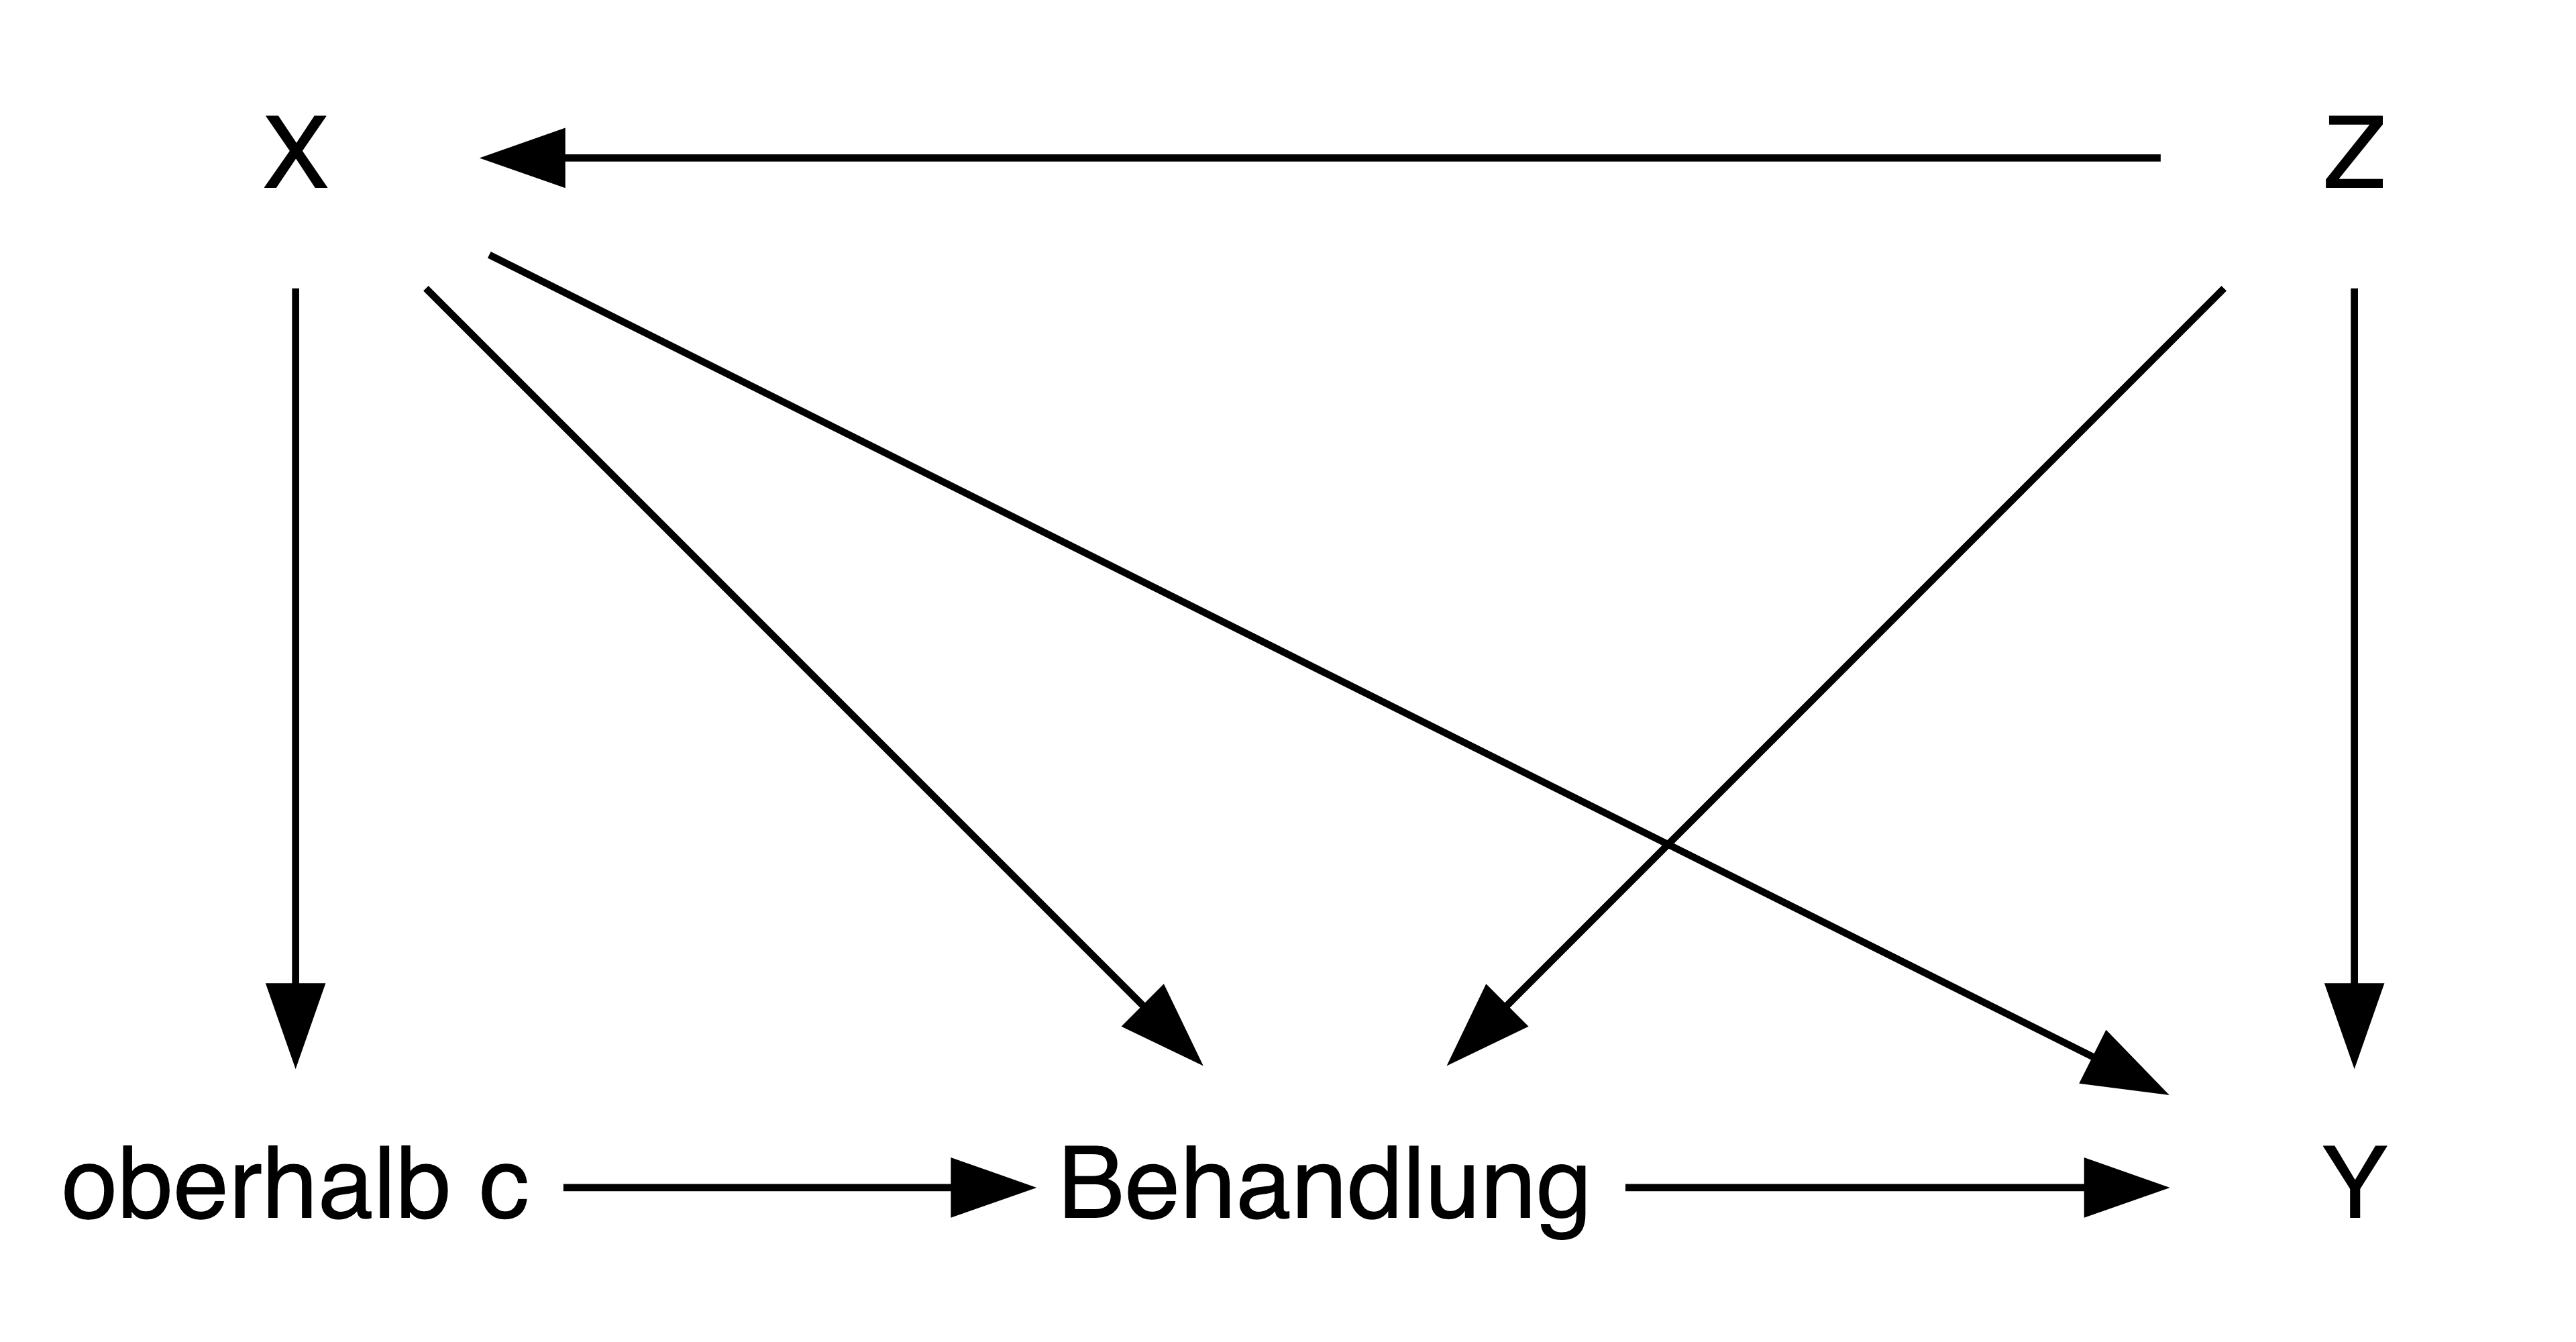
\includegraphics[width=5in,height=3in]{RDD_files/figure-latex/dot-figure-2.png}

}

\end{figure}

}

\caption{\label{fig-CDFRDD}Kausales Diagram für FRDD}

\end{figure}

Ein FRDD liegt vor, wenn die Zuweisung der Behandlung \(B\) durch die
Laufvariable \(X\) (und möglicherweise weitere Variablen \(Z\))
beeinflusst wird. Im Vergleich zum SRDD ist die Behandlung dann also
\emph{nicht} ausschließlich durch Überschreiten des Schwellenwerts
\(X = c\) bestimmt.

Abbildung~\ref{fig-CDFRDD} zeigt den grundsätzlichen Zusammenhang. Hier
genügt es weiterhin für \(X\) (und ggf. \(Z\)) zu kontrollieren, um den
Pfad \emph{oberhalb \(C\) → Behandlung \(B\) → \(Y\)} zu isolieren. Der
so für \emph{Behandlung \(B\)} ermittelte Effekt auf \(Y\) entspricht
jedoch \emph{nicht} dem ``vollständigen'' Behandlungseffekt, da bei
\(c\) die Zuweisung der Behandlung nicht von \(0\) auf \(100\%\)
springt. Die Schätzung des FRDD berücksichtigt dies und skaliert den
geschätzten Effekt entsprechend.

Wir betrachten zunächst den Zusammenhang \begin{align}
  Y_i = \beta_0 + \beta_1 B_i + \beta_2 (X_i - c) + u_i.\label{eq-simpleFRDD}
\end{align} In einem FRDD springt die Behandlungswahrscheinlichkeit am
Schwellenwert \(c\) um \(\Delta p<1\). Wir können \(B\) also nicht als
deterministische Funktion von \(X\), welche die Zuweisung zu
Behandlungs- bzw. Kontrollgruppe am Schwellenwert \(c\) anzeigt (wie im
SRDD), definieren. Stattdessen betrachten wir \begin{align}
  P(B_i=1\vert X_i) = 
  \begin{cases}
    g_{X_i<c}(X_i), & X_i < c \\ 
    g_{X_i\geq c}(X_i) & X_i \geq c
  \end{cases}\,. \label{eq-BFRDD}
\end{align} Die Funktionen \(g_{X_i<c}\) und \(g_{X_i\geq c}\) können
verschieden sein. Es muss jedoch
\[g_{X_i<c}(X_i = c) \neq g_{X_i\geq c}(X_i = c)\] gelten. Die
Behandlungsvariable \(B_i\) ist im FRDD also eine (binäre)
Zufallsvariable, deren bedingte Wahrscheinlichkeitsfunktion
\(P(B_i=1\vert X_i)\) am Schwellenwert \(c\) eine Diskontinuität
aufweist. Abbildung~\ref{fig-FRDDprobD} zeigt heispielhafte Verläufe
nicht-linearer bedingter Wahrscheinlichkeitsfunktion für die Behandlung
mit einer Diskontinuität bei \(X_i = c\).

\begin{Shaded}
\begin{Highlighting}[]
\FunctionTok{library}\NormalTok{(ggplot2)}
\FunctionTok{library}\NormalTok{(cowplot)}

\CommentTok{\# Bedingte Behandlungswahrscheinlichkeit im FRDD illustrieren}
\FunctionTok{ggplot}\NormalTok{() }\SpecialCharTok{+} 
  \FunctionTok{geom\_function}\NormalTok{(}
    \AttributeTok{fun =} \SpecialCharTok{\textasciitilde{}} \FunctionTok{ifelse}\NormalTok{(}
\NormalTok{      . }\SpecialCharTok{\textless{}} \DecValTok{0}\NormalTok{, }
      \SpecialCharTok{{-}}\NormalTok{.}\DecValTok{1} \SpecialCharTok{*}\NormalTok{ .}\SpecialCharTok{\^{}}\DecValTok{2} \SpecialCharTok{+}\NormalTok{ .}\DecValTok{25}\NormalTok{, }
      \SpecialCharTok{{-}}\NormalTok{.}\DecValTok{1} \SpecialCharTok{*}\NormalTok{ (.}\SpecialCharTok{{-}}\FloatTok{1.5}\NormalTok{)}\SpecialCharTok{\^{}}\DecValTok{2} \SpecialCharTok{+} \DecValTok{1}
\NormalTok{    ), }
    \AttributeTok{n =} \DecValTok{1000}
\NormalTok{  ) }\SpecialCharTok{+} 
    \FunctionTok{geom\_function}\NormalTok{(}
    \AttributeTok{fun =} \SpecialCharTok{\textasciitilde{}} \FunctionTok{ifelse}\NormalTok{(}
\NormalTok{      . }\SpecialCharTok{\textless{}} \DecValTok{0}\NormalTok{, }
\NormalTok{     .}\DecValTok{35}\NormalTok{, }
\NormalTok{     .}\DecValTok{65}
\NormalTok{    ),}
    \AttributeTok{n =} \DecValTok{1000}\NormalTok{, }
    \AttributeTok{lty =} \DecValTok{2}\NormalTok{, }
    \AttributeTok{col =} \StringTok{"red"}
\NormalTok{  ) }\SpecialCharTok{+} 
  \FunctionTok{scale\_x\_continuous}\NormalTok{(}
    \AttributeTok{name =} \StringTok{"Laufvariable X"}\NormalTok{, }
    \AttributeTok{limits =} \FunctionTok{c}\NormalTok{(}\SpecialCharTok{{-}}\FloatTok{1.5}\NormalTok{, }\FloatTok{1.5}\NormalTok{),}
    \AttributeTok{labels =} \ConstantTok{NULL}\NormalTok{,}
    \AttributeTok{breaks =} \ConstantTok{NULL}
\NormalTok{  ) }\SpecialCharTok{+}
  \FunctionTok{scale\_y\_continuous}\NormalTok{(}
    \AttributeTok{name =} \StringTok{"P(D=1|X)"}\NormalTok{, }
    \AttributeTok{breaks =} \FunctionTok{c}\NormalTok{(}\DecValTok{0}\NormalTok{, }\DecValTok{1}\NormalTok{), }
    \AttributeTok{limits =} \FunctionTok{c}\NormalTok{(}\DecValTok{0}\NormalTok{, }\DecValTok{1}\NormalTok{)}
\NormalTok{  ) }\SpecialCharTok{+}
  \FunctionTok{theme\_cowplot}\NormalTok{()}
\end{Highlighting}
\end{Shaded}

\begin{figure}[t]

{\centering 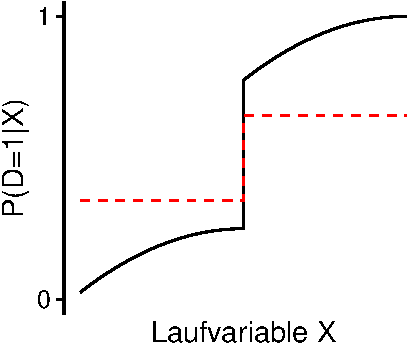
\includegraphics{RDD_files/figure-pdf/fig-FRDDprobD-1.pdf}

}

\caption{\label{fig-FRDDprobD}Bedingte Behandlungswahrscheinlichkeiten
im FRDD}

\end{figure}

Definition \eqref{eq-BFRDD} bedeutet, dass eine KQ-Schätzung von
\(\beta_1\) anhand \eqref{eq-simpleFRDD} eine \emph{verzerrte} Schätzung
des Behandlungseffekts ist: Der in \(\widehat{\beta}_1\) erfasste Effekt
auf \(Y\) ist auf einen Sprung der Behandlungswahrscheinlichkeit bei
\(X_i = c\) um \emph{weniger} als \(100\%\) zurückzuführen. Der wahre
Behandlungseffekt wird also \emph{unterschätzt}. Daher muss
\(\widehat{\beta}_1\) skaliert werden, sodass die Schätzung als Effekt
einer Änderung der Behandlungswahrscheinlichkei um \(100\%\)
interpretiert werden kann --- der erwartete Effekt, wenn ausschließlich
Subjekte mit \(X_i\geq c\) behandelt würden. Diese skalierte Schätzung
erhalten wir mit IV-Regression (vgl. Kapitel XYZ). Hierfür nutzen wir
für \(B_i\) die Instrumentvariable \begin{align*}
  D_i = \begin{cases}
    0, & X_i < c \\ 
    1, & X_i \geq c.
  \end{cases}
\end{align*}

Angenommen \(g_{X_i\geq c}(X_i) = \alpha_0\) und
\(g_{X_i<c}(X_i) = \alpha_0 + \alpha_1\) mit \(\alpha_0 + \alpha_1 < 1\)
(vgl. rote Funktion in Abbildung~\ref{fig-CDFRDD}). Der FRDD-Schätzer
des Behandlungseffekts ist dann \(\widehat{\gamma}_\textup{FRDD}\) im
2SLS-Verfahren mit den Regressionen \begin{align}
  \begin{split}
  (\mathrm{I})\qquad B_i =&\, \alpha_0 + \alpha_1 D_i + \alpha_2 (X_i - c) + e_i,\\
  (\mathrm{II})\qquad Y_i =&\, \gamma_0 + \gamma_1 \widehat{B}_i + \gamma_2 (X_i - c) + \epsilon_i,
  \end{split}\label{eq:FRDD_simpleIV}
\end{align} wobei \(\widehat{B}_i\) die angepassten Werte aus Stufe
\((\mathrm I)\) und \(e_i\) sowie \(\epsilon_i\) Fehlterterme sind.

Analog zum SRDD müssen in empirischen Anwendungen geeignete
Spezifikationen für die Regressionsfunktionen \eqref{eq-simpleFRDD} und
\eqref{eq-BFRDD} gewählt und der 2SLS-Schätzer \eqref{eq:FRDD_simpleIV}
entsprechend angepasst werden. Ein einfaches Interaktionsmodell wäre
\begin{align}
  \begin{split}
  (\mathrm{I})\qquad B_i =&\, \alpha_0 + \alpha_1 D_i + \alpha_2 (X_i - c)\\ 
  +&\, \alpha_3 (X_i - c) \times D_i + e_i,\\
  \\
  (\mathrm{II})\qquad Y_i =&\, \gamma_0 + \gamma_1 \widehat{B}_i\\
  +&\, \gamma_2 (X_i - c) + \gamma_3 (X_i-c)\times\widehat{B}_i, \epsilon_i
  \end{split},\label{eq:FRDD_lintIV}
\end{align} d.h. wir instrumentieren \(B_i\) mit \(D_i\) und dem
Interaktionsterm \((X_i-c)\times D_i\).

Wie im SRDD werden die IV-Ansätze für das FRDD \eqref{eq:FRDD_simpleIV}
und \eqref{eq:FRDD_lintIV} in empirischen Studien unter Berücksichtigung
einer Bandweite (i.d.R. dieselbe Bandweite für beide Stufen) angewendet.

\hypertarget{case-study-protestantische-arbeitsethik}{%
\section{Case Study: Protestantische
Arbeitsethik}\label{case-study-protestantische-arbeitsethik}}

Die Studie \emph{Beyond Work Ethic: Religion, Individual, and Political
Preferences} (Basten und Betz 2013) untersucht den Zusammenhang zwischen
Religion, individuellen Merkmalen und politischen Präferenzen. Das
Hauptaugenmerk ist die Rolle von Religiosität als Einflussfaktor auf
politische Einstellungen. Die Hypothese der Autoren ist, dass
Religiosität eines Individuums über den traditionellen Rahmen von
Moralvorstellungen und sozialen Normen hinaus auch die politischen
Präferenzen beeinflusst. Eine entsprechende Theorie wurde zu Beginn des
20. Jahrhunderts entwickelt und prominent von Max Weber (vgl. Weber
2004) vertreten. Weber argumentiert, dass die protestantische
Arbeitsethik einen entscheidenden Einfluss auf die Entwicklung des
Kapitalismus hatte. Laut Weber führte der protestantische Glaube an
harte Arbeit, ein sparsames Leben und ethisches Verhalten zur einer in
den damaligen Gesellschaften weit verbreiteten Geisteshaltung, die
wirtschaftliches Wachstum förderte und den Aufstieg des Kapitalismus
begünstigte.

Basten und Betz (2013) nutzen Wahlergebnisse sowie geo- und
soziodemographische Datensätze für schweizer Gemeinden, um den
Zusammenhang zwischen Religiosität und politischen Präferenzen wie
links-rechts-Ausrichtung, Einstellungen zur Umverteilung und
Einwanderung zu untersuchen. Hierfür verwenden die Autoren ein FRDD,
dass eine historisch bedingte Diskontinuität der geographischen
Verteilung von evanglischer bzw. katholischer Religionszugehörigkeit
zwischen den Kantonen Freiburg (überwiegend dunkelrote Region, frz.
\emph{Fribourg}) und Waadt (kleinere hellrote Region, frz. \emph{Vaud})
ausnutzt. Die historische Verteilung der Konfessionen in der
betrachteten Region im 16. Jahrhundert durch Abspaltung des Kantons
Freiburg ist in Abbildung~\ref{fig-vaudfb} dargestellt.

Aufgrund von Bevölkerungsbewegungen ist die Verteilung der Konfessionen
zwar nicht mehr eindeutig durch die Kantonsgrenze bestimmt, jedoch sind
die Gemeinden der betrachteten Kantone auch heute noch mehrheitlich
protestantisch bzw. katholisch. Es ist plausibel, dass eine Prägung
gemäß Webers Theorie vorliegt, sich die Gemeinden nahe der Grenz aber
hinsichtlich anderer Charakteristika (insb. der Bevölkerungsstruktur)
nicht systematisch unterscheiden. Somit liegt ein quai

\begin{figure}[t]

\sidecaption{\label{fig-vaudfb}Historische Verteilung von
Religionszugehörigkeit in Schweizer Gemeinden im 16. Jahrhundert.
Quelle: Basten und Betz (2013).}

{\centering 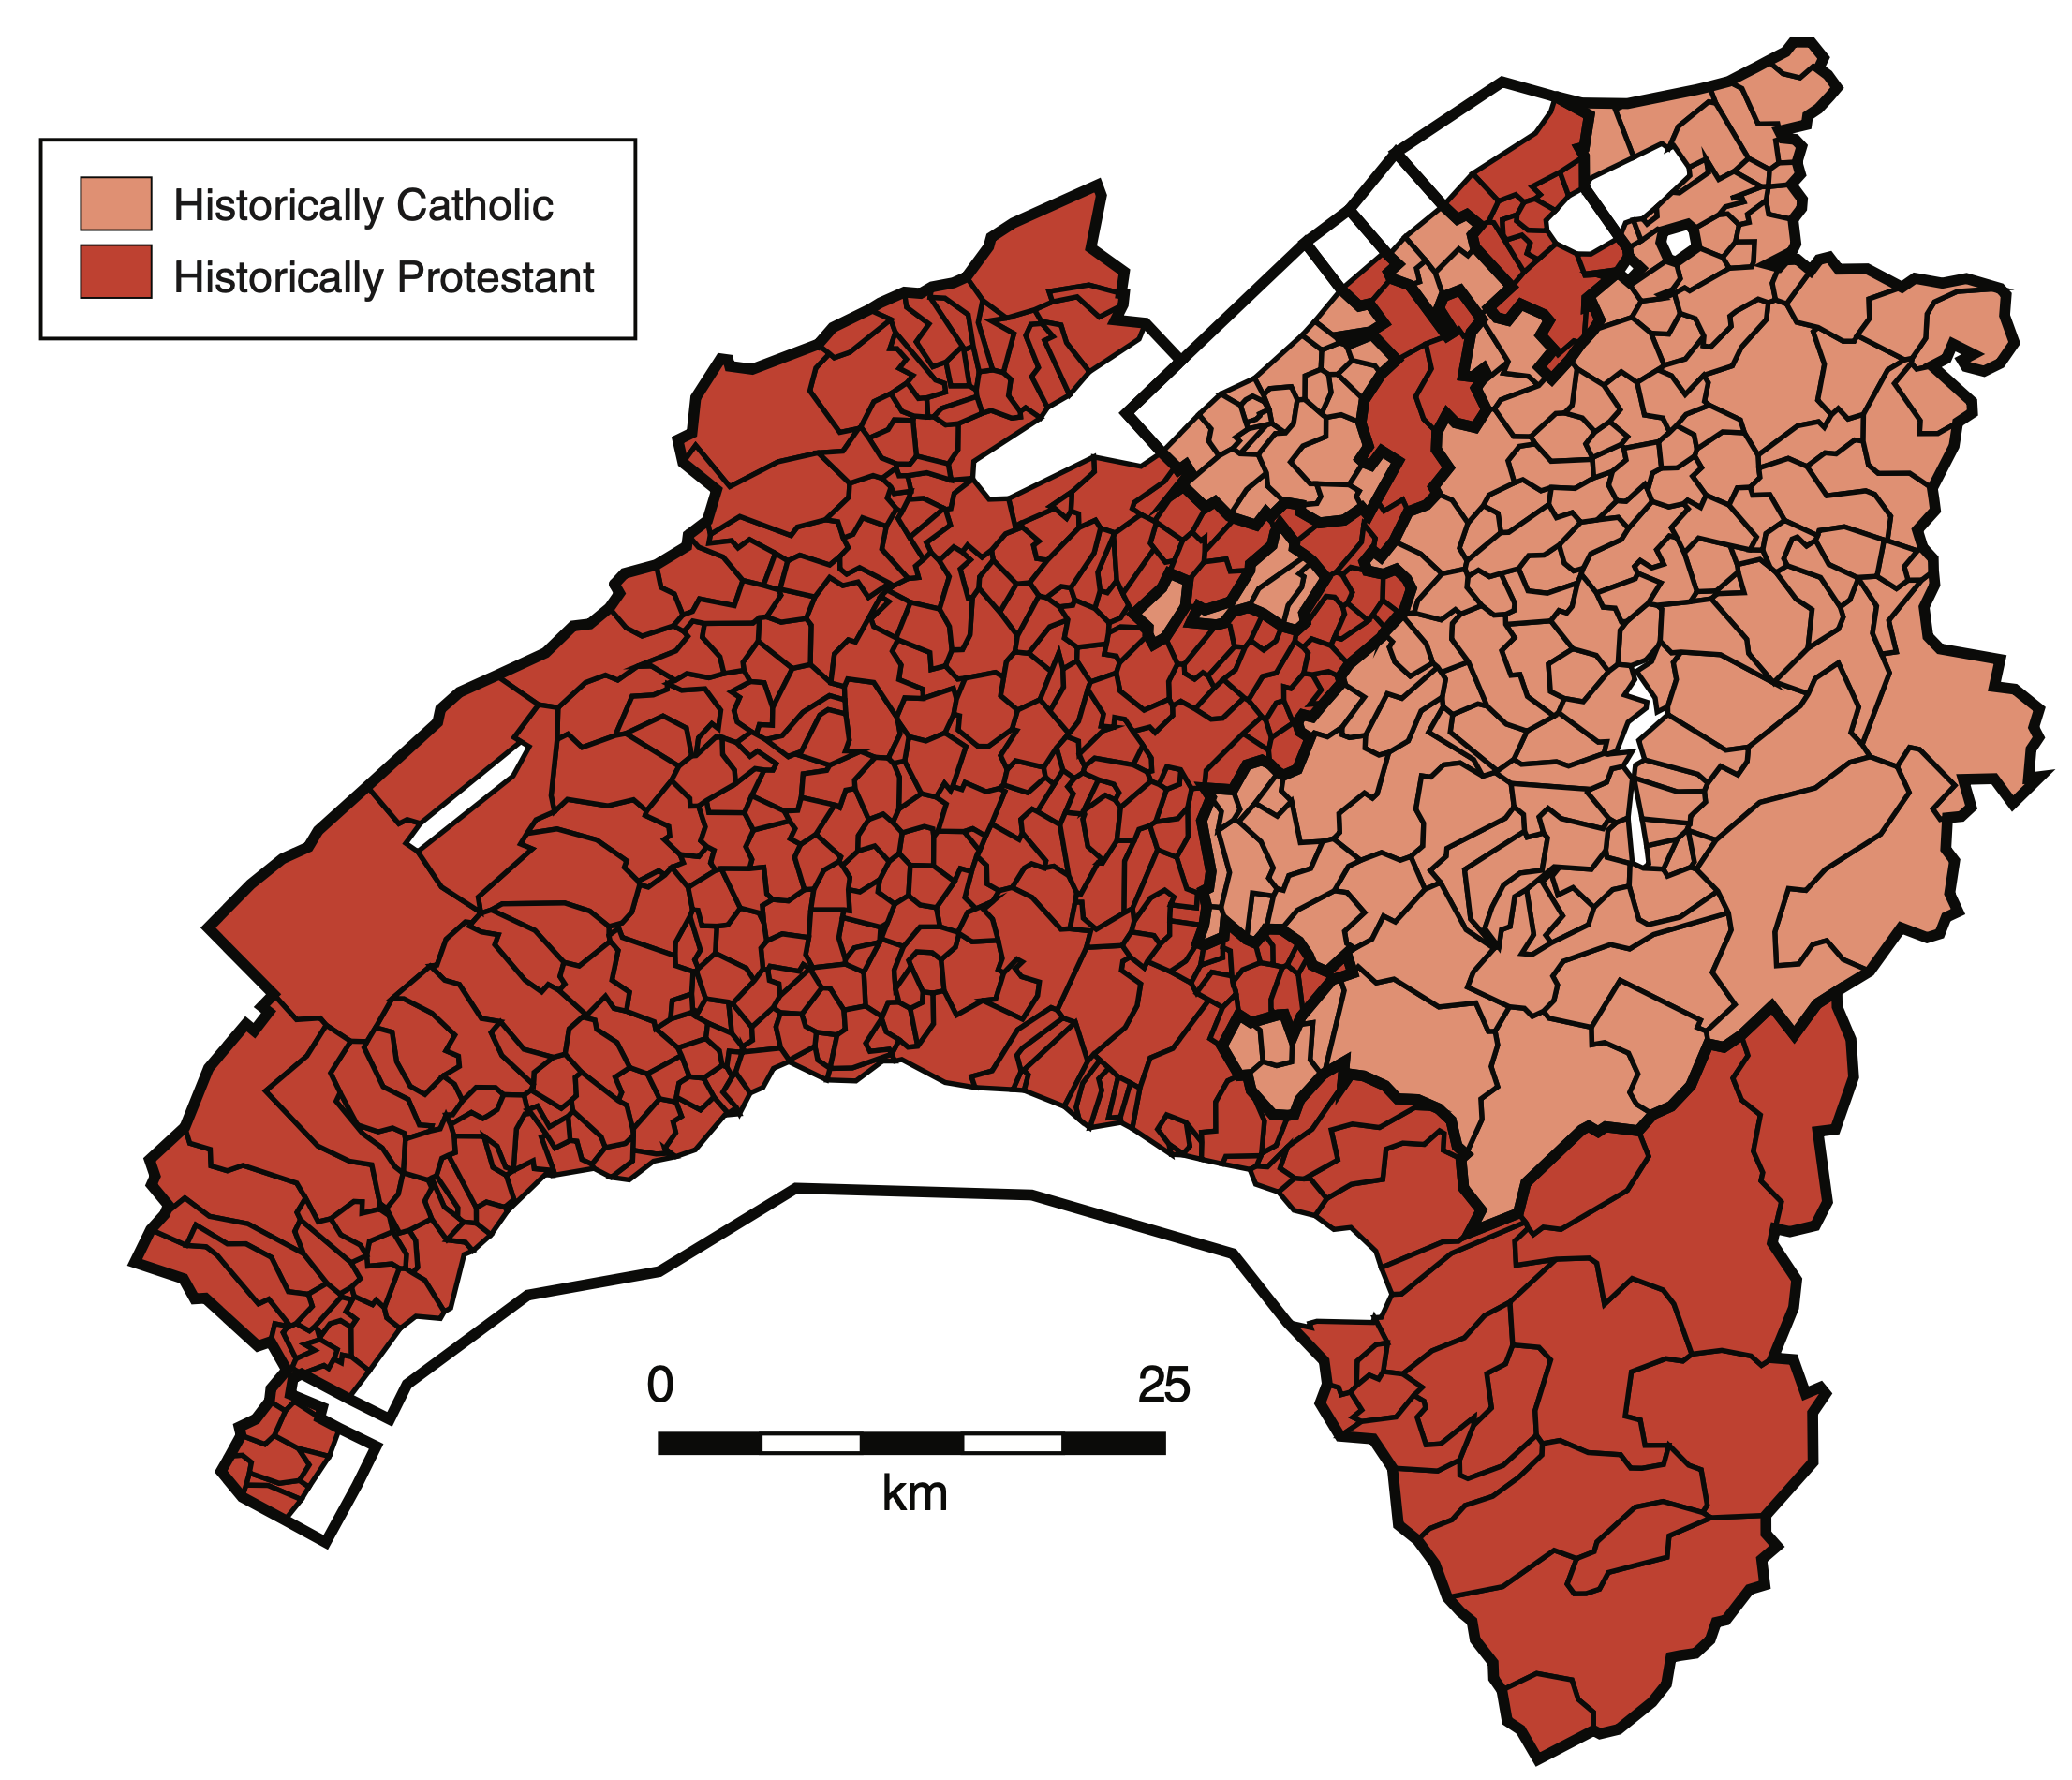
\includegraphics[width=4.16667in,height=\textheight]{img/WaadtFribourg.png}

}

\end{figure}

Die Ergebnisse der Studie zeigen einen signifikanten Einfluss von
Protestantismus auf politische Präferenzen, die über traditionelle
Moralvorstellungen hinausgehen: Die Autoren finden Hinweise, dass
Einwohner evangelisch geprägter Gemeinden eher konservative soziale und
politische Ansichten vertreten. Eine mögliche Erklärung für diesen
Effekt ist, dass religiöse Institutionen auch eine soziale und
politische Agenda verfolgen, die von den Gläubigen internalisiert wird.

\hypertarget{aufbereitung-der-daten}{%
\subsection{Aufbereitung der Daten}\label{aufbereitung-der-daten}}

In diesem Kapitel zeigen wir, wie die Kernergebnisse der Studie mit R
reproduziert werden können. Hierfür werden folgende Pakete benötigt.

\begin{Shaded}
\begin{Highlighting}[]
\FunctionTok{library}\NormalTok{(tidyverse)}
\FunctionTok{library}\NormalTok{(haven)}
\FunctionTok{library}\NormalTok{(vtable)}
\FunctionTok{library}\NormalTok{(rdrobust)}
\end{Highlighting}
\end{Shaded}

Das Papier sowie der Datensatz \texttt{BastenBetz.dta} sind auf der
\href{https://www.aeaweb.org/articles?id=10.1257/pol.5.3.67}{Übersichtsseite
der AEA} verfügbar und liegt im STATA-Format \texttt{.dta}
vor.\footnote{Siehe alternativ das
  \href{https://papers.ssrn.com/sol3/papers.cfm?abstract_id=2133848}{working
  paper}, falls kein Abbonement für AEA-Journals vorliegt.}

\begin{Shaded}
\begin{Highlighting}[]
\CommentTok{\# Datensatz einlesen}
\NormalTok{BastenBetz }\OtherTok{\textless{}{-}} \FunctionTok{read\_dta}\NormalTok{(}\StringTok{\textquotesingle{}BastenBetz.dta\textquotesingle{}}\NormalTok{)}
\end{Highlighting}
\end{Shaded}

Der Datensatz \texttt{BastenBetz} enthält Beobachtungen zu 509 schweizer
Gemeinden. Eine Vielzahl an Variablen ist lediglich für
Robustheits-Checks relevant. Für die Reproduktion der Kernergebnisse
erstellen wir zunächst einen reduzierten Datensatz und transformieren
einige Variablen.

\begin{Shaded}
\begin{Highlighting}[]
\CommentTok{\# Reduzierten Datensatz erstellen}
\NormalTok{BastenBetz }\OtherTok{\textless{}{-}}\NormalTok{ BastenBetz }\SpecialCharTok{\%\textgreater{}\%}
  \FunctionTok{transmute}\NormalTok{(}
    \AttributeTok{gini =}\NormalTok{ Ecoplan\_gini,}
    \AttributeTok{prot =}\NormalTok{ prot1980s,}
    \AttributeTok{bord =}\NormalTok{ borderdis, }
\NormalTok{    vaud,}
\NormalTok{    pfl, }
\NormalTok{    pfr, }
\NormalTok{    pfi}
\NormalTok{  )}
\end{Highlighting}
\end{Shaded}

Die Definitionen der Variablen sind in Tabelle~\ref{tbl-BastenBetzRed}
gegeben. Die Präferenzen \texttt{pfl}, \texttt{pfr} und \texttt{pfi}
basieren auf Wahlergebnissen auf Gemeindeebene zu Volksentscheiden.

\hypertarget{tbl-BastenBetzRed}{}
\begin{longtable}[]{@{}
  >{\raggedright\arraybackslash}p{(\columnwidth - 2\tabcolsep) * \real{0.1806}}
  >{\raggedright\arraybackslash}p{(\columnwidth - 2\tabcolsep) * \real{0.8194}}@{}}
\caption{\label{tbl-BastenBetzRed}\texttt{BastenBetz} -- Variablen und
Definitionen}\tabularnewline
\toprule\noalign{}
\begin{minipage}[b]{\linewidth}\raggedright
Variable
\end{minipage} & \begin{minipage}[b]{\linewidth}\raggedright
Definition
\end{minipage} \\
\midrule\noalign{}
\endfirsthead
\toprule\noalign{}
\begin{minipage}[b]{\linewidth}\raggedright
Variable
\end{minipage} & \begin{minipage}[b]{\linewidth}\raggedright
Definition
\end{minipage} \\
\midrule\noalign{}
\endhead
\bottomrule\noalign{}
\endlastfoot
\texttt{prot} & Anteil Prothestanten im Jahr 1980 (\%) \\
\texttt{gini} & Gini-Koeffizient \\
\texttt{bord} & Laufdistanz zur Kantonsgrenze (Km) \\
\texttt{vaud} & Dummyvariable: Gemeine im Kanton Waadt \\
\texttt{pfl} & Präferenz für Freizeit (\%) \\
\texttt{pfr} & Präferenz für Umverteilung (\%) \\
\texttt{pfi} & Präferenz für wirtschaftliche Intervention des Staats
(\%) \\
\end{longtable}

Für die Berechnung der optimalen Bandweite des FRDD verwenden wir einen
MSE-optimalen Schätzer, der in der Funktion
\texttt{rdrobust::rdbwselect()} implementiert ist.\footnote{Basten und
  Betz (2013) setzen BW = 5.01, den Durchschnitt von IK-Schätzungen über
  Modelle sämtlicher betrachteter Outcome-Variablen. Diese Bandweite
  liegt nahe des Ergebnisses von \texttt{rdbwselect}. Wir verwenden
  nachfolgend die Schätzung \texttt{OB}.}

\begin{Shaded}
\begin{Highlighting}[]
\CommentTok{\# Bandweite schätzen (Bsp. für Freizeitpräferenz)}
\NormalTok{bw\_selection }\OtherTok{\textless{}{-}} \FunctionTok{rdbwselect}\NormalTok{(}
  \AttributeTok{y =}\NormalTok{ BastenBetz}\SpecialCharTok{$}\NormalTok{pfl,}
  \AttributeTok{x =}\NormalTok{ BastenBetz}\SpecialCharTok{$}\NormalTok{bord,}
  \AttributeTok{fuzzy =}\NormalTok{ BastenBetz}\SpecialCharTok{$}\NormalTok{prot, }
  \AttributeTok{bwselect =} \StringTok{"mserd"}\NormalTok{, }
  \AttributeTok{kernel =} \StringTok{"uniform"}
\NormalTok{) }

\CommentTok{\# Bandweite auslesen und zuweisen}
\NormalTok{(OB }\OtherTok{\textless{}{-}}\NormalTok{ bw\_selection}\SpecialCharTok{$}\NormalTok{bws[}\DecValTok{1}\NormalTok{])}
\end{Highlighting}
\end{Shaded}

\begin{verbatim}
[1] 5.078001
\end{verbatim}

\hypertarget{deskriptive-statistiken}{%
\subsection{Deskriptive Statistiken}\label{deskriptive-statistiken}}

Zur Reproduktion von Tabelle 1 aus Basten und Betz (2013) erzeugen wir
eine nach Kantonen gruppierte Zusammenfassung der Daten und berechnen
deskriptive Statistiken. Wie im Paper berücksichtigen wir hierbei nur
Gemeinden innerhalb der geschätzten optimalen Bandweite \texttt{OB}.

\begin{Shaded}
\begin{Highlighting}[]
\CommentTok{\# Datensatz für Reproduktion von Table 1 formatieren}
\NormalTok{T1 }\OtherTok{\textless{}{-}}\NormalTok{ BastenBetz }\SpecialCharTok{\%\textgreater{}\%}
  \FunctionTok{filter}\NormalTok{(}\FunctionTok{abs}\NormalTok{(bord) }\SpecialCharTok{\textless{}}\NormalTok{ OB) }\SpecialCharTok{\%\textgreater{}\%}
  \FunctionTok{mutate}\NormalTok{(}
    \AttributeTok{vaud =} \FunctionTok{ifelse}\NormalTok{(}
      \AttributeTok{test =}\NormalTok{ vaud }\SpecialCharTok{==} \DecValTok{1}\NormalTok{, }
      \AttributeTok{yes =} \StringTok{"Waadt"}\NormalTok{, }
      \AttributeTok{no =} \StringTok{"Freiburg"}
\NormalTok{    ),}
    \AttributeTok{prot =}\NormalTok{ prot }\SpecialCharTok{*} \DecValTok{100}
\NormalTok{  ) }\SpecialCharTok{\%\textgreater{}\%}
  \FunctionTok{group\_by}\NormalTok{(vaud) }\SpecialCharTok{\%\textgreater{}\%}
  \FunctionTok{summarise}\NormalTok{(}
    \FunctionTok{across}\NormalTok{(}
      \FunctionTok{everything}\NormalTok{(), }
      \FunctionTok{list}\NormalTok{(}
        \AttributeTok{Mean =}\NormalTok{ mean, }
        \AttributeTok{SD =}\NormalTok{ sd, }
        \AttributeTok{N =}\NormalTok{ length}
\NormalTok{      )}
\NormalTok{    )}
\NormalTok{  ) }\SpecialCharTok{\%\textgreater{}\%}
  \FunctionTok{pivot\_longer}\NormalTok{(}
    \AttributeTok{cols =} \SpecialCharTok{{-}}\NormalTok{vaud,}
    \AttributeTok{names\_to =} \FunctionTok{c}\NormalTok{(}\StringTok{"variable"}\NormalTok{, }\StringTok{"statistic"}\NormalTok{), }
    \AttributeTok{names\_sep =} \StringTok{"\_"}
\NormalTok{  )}
\end{Highlighting}
\end{Shaded}

Für die tabellarische Darstellung transformieren wir in ein weites
Format, sodass die Tabelle die deskriptive Statistiken spaltenweise für
die Kantone zeigt.

\begin{Shaded}
\begin{Highlighting}[]
\CommentTok{\# Daten in weites Format überführen}
\NormalTok{T1\_wider }\OtherTok{\textless{}{-}}\NormalTok{ T1 }\SpecialCharTok{\%\textgreater{}\%} 
  \FunctionTok{pivot\_wider}\NormalTok{(}
    \AttributeTok{names\_from =} \FunctionTok{c}\NormalTok{(}\StringTok{"vaud"}\NormalTok{, }\StringTok{"statistic"}\NormalTok{)}
\NormalTok{  )}
\end{Highlighting}
\end{Shaded}

Die Tabelle erzeugen wir mit \texttt{gt::gt()}.

\begin{Shaded}
\begin{Highlighting}[]
\CommentTok{\# Tabelle mit gt() erzeugen}
\NormalTok{T1\_wider }\SpecialCharTok{\%\textgreater{}\%}
  \FunctionTok{gt}\NormalTok{(}\AttributeTok{rowname\_col =} \StringTok{"Variable"}\NormalTok{) }\SpecialCharTok{\%\textgreater{}\%} 
  \FunctionTok{tab\_spanner\_delim}\NormalTok{(}
    \AttributeTok{delim =} \StringTok{"\_"}\NormalTok{,}
\NormalTok{  ) }\SpecialCharTok{\%\textgreater{}\%}
\NormalTok{ tabopts}
\end{Highlighting}
\end{Shaded}

\hypertarget{tbl-sumstat}{}
\begin{longtable}{lrrrrrr}
\caption{\label{tbl-sumstat}Datensatz \texttt{BastenBetz} -- Zusammenfassende Statistiken }\tabularnewline

\toprule
 & \multicolumn{3}{c}{Freiburg} & \multicolumn{3}{c}{Waadt} \\ 
\cmidrule(lr){2-4} \cmidrule(lr){5-7}
variable & Mean & SD & N & Mean & SD & N \\ 
\midrule\addlinespace[2.5pt]
gini & $0.302$ & $0.029$ & $49$ & $0.367$ & $0.052$ & $84$ \\ 
prot & $9.428$ & $5.695$ & $49$ & $83.245$ & $11.411$ & $84$ \\ 
bord & $-2.327$ & $1.274$ & $49$ & $2.493$ & $1.201$ & $84$ \\ 
pfl & $48.239$ & $4.774$ & $49$ & $39.508$ & $5.723$ & $84$ \\ 
pfr & $43.049$ & $2.634$ & $49$ & $39.19$ & $5.025$ & $84$ \\ 
pfi & $52.642$ & $2.94$ & $49$ & $47.086$ & $3.368$ & $84$ \\ 
\bottomrule
\end{longtable}

Die Statistiken in Tabelle~\ref{tbl-sumstat} scheinen konsistent mit der
(historischen) Verteilung der Religionszugehörigkeit und politischen
Einstellung gemäß der Hypothese: Im überwiegend katholischen Freiburg
finden wir eine größere Einkommensungleichkeit und höhere aus
Wahlergebnissen abgeleitete Präferenzen für Freizeit, Umverteilung sowie
staatliche Interventionen.

\hypertarget{modellspezifikation-und-first-stage-ergebnisse}{%
\subsection{Modellspezifikation und
First-Stage-Ergebnisse}\label{modellspezifikation-und-first-stage-ergebnisse}}

Die Kantone Waadt und Freiburg haben bis heute mehrheitlich
protestantische bzw. katholische Gemeinden. Die Verteilung von
Protestantismus ist also, u.a. aufgrund von Bevölkerungsbewegungen,
nicht mehr deterministisch. An der Kantonsgrenze besteht jedoch eine
deutliche Diskontinuität im Anteil protestantischer Einwohner, die auf
die historische Verteilung der Religionszugehörigkeit zurückzuführen
ist. Damit kann ein FRDD implementiert werden, bei dem die Distanz zur
Grenze (\texttt{bord}) die zentrierte Laufvariable ist und die
Zugehörigkeit zum Kanton Waadt (\texttt{vaud}) ein Instrument für die
Behandlungsvariable (\texttt{prot}) ist.

Wir nutzen die Funktion \texttt{rdrobust::rdplot} um diesen Zusammenhang
für verschiedene Bandweiten anhand des linearen Interaktionsmodells
\begin{align}
  \begin{split}
  prot_i =&\, \alpha_0 + \alpha_1 vaud_i + \alpha_2 bord_i \\
  +&\, \alpha_3 bord_i \times vaud_i + u_i
  \end{split}\label{eq:BBFSR}
\end{align} grafisch darzustellen. Dies ist die First-Stage-Regression
für die 2SLS-Schätzung der Behandlungseffekte.

\begin{Shaded}
\begin{Highlighting}[]
\CommentTok{\# Reproduktion von Abbildung 3 in Basten und Betz (2013)}
\NormalTok{plots\_BB }\OtherTok{\textless{}{-}} \FunctionTok{list}\NormalTok{(}
  \CommentTok{\# gesch. optimale Bandweite}
  \AttributeTok{p\_OB =} \FunctionTok{rdplot}\NormalTok{(}
    \AttributeTok{y =}\NormalTok{ BastenBetz}\SpecialCharTok{$}\NormalTok{prot, }
    \AttributeTok{x =}\NormalTok{ BastenBetz}\SpecialCharTok{$}\NormalTok{bord, }
    \AttributeTok{h =} \FunctionTok{c}\NormalTok{(OB, OB), }
    \AttributeTok{x.label =} \StringTok{"Distanz zur Grenze (bord)"}\NormalTok{,}
    \AttributeTok{y.label =} \StringTok{"Anteil Protestanten (prot)"}\NormalTok{, }
    \AttributeTok{title =} \StringTok{"Gesch. Bandweite"}\NormalTok{,}
    \AttributeTok{p =} \DecValTok{1}\NormalTok{, }
    \AttributeTok{nbins =} \FunctionTok{c}\NormalTok{(}\DecValTok{6}\NormalTok{, }\DecValTok{14}\NormalTok{), }
    \AttributeTok{masspoints =} \StringTok{"off"}
\NormalTok{  ),}
  
  \CommentTok{\# Bandweite 10}
  \AttributeTok{p\_BW10 =} \FunctionTok{rdplot}\NormalTok{(}
    \AttributeTok{y =}\NormalTok{ BastenBetz}\SpecialCharTok{$}\NormalTok{prot, }
    \AttributeTok{x =}\NormalTok{ BastenBetz}\SpecialCharTok{$}\NormalTok{bord, }
    \AttributeTok{h =} \FunctionTok{c}\NormalTok{(}\DecValTok{10}\NormalTok{, }\DecValTok{10}\NormalTok{), }
    \AttributeTok{x.label =} \StringTok{"Distanz zur Grenze (bord)"}\NormalTok{,}
    \AttributeTok{y.label =} \StringTok{"Anteil Protestanten  (prot)"}\NormalTok{, }
    \AttributeTok{title =} \StringTok{"Bandweite = 10"}\NormalTok{,}
    \AttributeTok{p =} \DecValTok{1}\NormalTok{, }
    \AttributeTok{nbins =} \FunctionTok{c}\NormalTok{(}\DecValTok{6}\NormalTok{, }\DecValTok{14}\NormalTok{),}
    \AttributeTok{masspoints =} \StringTok{"off"}
\NormalTok{  ),}
  
  \CommentTok{\# Bandweite 20}
  \AttributeTok{p\_BW20 =} \FunctionTok{rdplot}\NormalTok{(}
    \AttributeTok{y =}\NormalTok{ BastenBetz}\SpecialCharTok{$}\NormalTok{prot, }
    \AttributeTok{x =}\NormalTok{ BastenBetz}\SpecialCharTok{$}\NormalTok{bord, }
    \AttributeTok{h =} \FunctionTok{c}\NormalTok{(}\DecValTok{20}\NormalTok{, }\DecValTok{20}\NormalTok{), }
    \AttributeTok{x.label =} \StringTok{"Distanz zur Grenze (bord)"}\NormalTok{,}
    \AttributeTok{y.label =} \StringTok{"Anteil Protestanten  (prot)"}\NormalTok{, }
    \AttributeTok{title =} \StringTok{"Bandweite = 20"}\NormalTok{,}
    \AttributeTok{p =} \DecValTok{1}\NormalTok{, }
    \AttributeTok{nbins =} \FunctionTok{c}\NormalTok{(}\DecValTok{6}\NormalTok{, }\DecValTok{14}\NormalTok{),}
    \AttributeTok{masspoints =} \StringTok{"off"}
\NormalTok{  ),}
  
  \CommentTok{\# Gesamter Datensatz}
  \AttributeTok{p\_G =} \FunctionTok{rdplot}\NormalTok{(}
    \AttributeTok{y =}\NormalTok{ BastenBetz}\SpecialCharTok{$}\NormalTok{prot, }
    \AttributeTok{x =}\NormalTok{ BastenBetz}\SpecialCharTok{$}\NormalTok{bord,}
    \AttributeTok{x.label =} \StringTok{"Distanz zur Grenze (bord)"}\NormalTok{,}
    \AttributeTok{y.label =} \StringTok{"Anteil Protestanten"}\NormalTok{, }
    \AttributeTok{title =} \StringTok{"Ges. Datensatz"}\NormalTok{,}
    \AttributeTok{p =} \DecValTok{1}\NormalTok{, }
    \AttributeTok{nbins =} \FunctionTok{c}\NormalTok{(}\DecValTok{6}\NormalTok{, }\DecValTok{14}\NormalTok{),}
    \AttributeTok{masspoints =} \StringTok{"off"}
\NormalTok{  )}
\NormalTok{)}
\end{Highlighting}
\end{Shaded}

Wir sammeln die Ergebnisse in einem Plot-Gitter mit
\texttt{cowplot::plot\_grid()}.

\begin{Shaded}
\begin{Highlighting}[]
\CommentTok{\# Reproduktion von Abbildung 3 in Basten und Betz (2013)}
\FunctionTok{plot\_grid}\NormalTok{(}
  \AttributeTok{plotlist =} \FunctionTok{map}\NormalTok{(plots\_BB, }\SpecialCharTok{\textasciitilde{}}\NormalTok{ .}\SpecialCharTok{$}\NormalTok{rdplot), }\AttributeTok{ncol =} \DecValTok{2}
\NormalTok{)}
\end{Highlighting}
\end{Shaded}

\begin{figure}[t]

{\centering 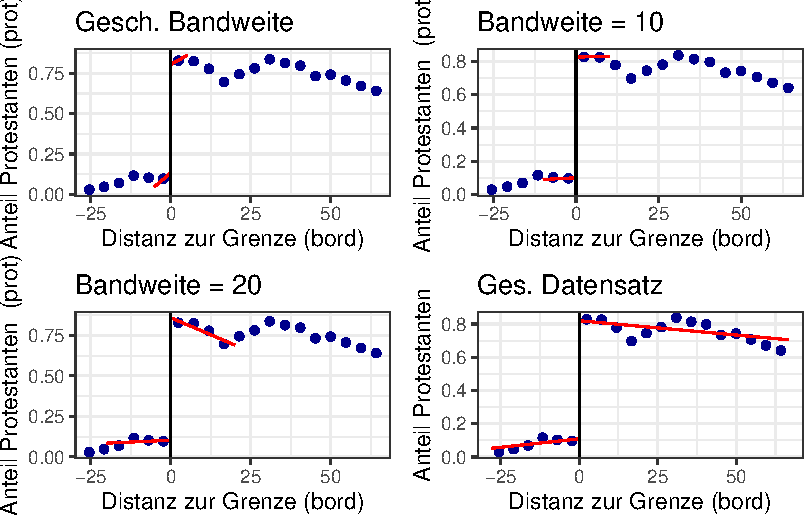
\includegraphics{RDD_files/figure-pdf/fig-BastenBetzFS-1.pdf}

}

\caption{\label{fig-BastenBetzFS}First-Stage-Regressionen}

\end{figure}

Die Grafiken in Abbildung~\ref{fig-BastenBetzFS} zeigen deutliche
Hinweise auf die Diskontinuität in \texttt{prot} nahe der Kantonsgrenze.
Die Größe des geschätzten Sprungs scheint nur wenig sensitiv gegenüber
der gewählten Bandweite zu sein. Die Signifikanz des Effekts können wir
anhand der jeweiligen KQ-Regressionen beurteilen.\footnote{Wir nutzen
  \texttt{update()} um die Regression mit weniger Code für verschiedene
  Bandweiten zu schätzen.}

\begin{Shaded}
\begin{Highlighting}[]
\CommentTok{\# Reproduktion der First{-}Stage{-}Regressionen}
\CommentTok{\# s. Tabelle 2 in Basten und Betz (2013)}

\CommentTok{\# (1) BW = OB}
\NormalTok{FS1 }\OtherTok{\textless{}{-}} \FunctionTok{lm}\NormalTok{(}
  \AttributeTok{formula =}\NormalTok{ prot }\SpecialCharTok{\textasciitilde{}}\NormalTok{ vaud }\SpecialCharTok{+}\NormalTok{ bord }\SpecialCharTok{+}\NormalTok{ vaud }\SpecialCharTok{*}\NormalTok{ bord, }
  \AttributeTok{data =}\NormalTok{ BastenBetz }\SpecialCharTok{\%\textgreater{}\%} 
    \FunctionTok{filter}\NormalTok{(}
      \FunctionTok{abs}\NormalTok{(bord) }\SpecialCharTok{\textless{}=}\NormalTok{ OB}
\NormalTok{    )}
\NormalTok{)}

\CommentTok{\# (2) BW = 10}
\NormalTok{FS2 }\OtherTok{\textless{}{-}} \FunctionTok{update}\NormalTok{(}
\NormalTok{  FS1,}
  \AttributeTok{data =}\NormalTok{ BastenBetz }\SpecialCharTok{\%\textgreater{}\%} 
    \FunctionTok{filter}\NormalTok{(}
      \FunctionTok{abs}\NormalTok{(bord) }\SpecialCharTok{\textless{}=} \DecValTok{10}
\NormalTok{    )}
\NormalTok{)}

\CommentTok{\# (3) BW = 20}
\NormalTok{FS3 }\OtherTok{\textless{}{-}} \FunctionTok{update}\NormalTok{(}
\NormalTok{  FS1,}
  \AttributeTok{data =}\NormalTok{ BastenBetz }\SpecialCharTok{\%\textgreater{}\%}
    \FunctionTok{filter}\NormalTok{(}
      \FunctionTok{abs}\NormalTok{(bord) }\SpecialCharTok{\textless{}=} \DecValTok{20}
\NormalTok{    )}
\NormalTok{)}

\CommentTok{\# (4) Ges. Datensatz}
\NormalTok{FS4 }\OtherTok{\textless{}{-}} \FunctionTok{update}\NormalTok{(}
  \AttributeTok{object =}\NormalTok{ FS1,}
  \AttributeTok{data =}\NormalTok{ BastenBetz}
\NormalTok{)}
\end{Highlighting}
\end{Shaded}

\begin{Shaded}
\begin{Highlighting}[]
\CommentTok{\# Tabellarische Darstellung}
\FunctionTok{modelsummary}\NormalTok{(}
  \FunctionTok{list}\NormalTok{(}
    \StringTok{"BW = OB"}\OtherTok{=}\NormalTok{ FS1, }
    \StringTok{"BW = 10"} \OtherTok{=}\NormalTok{ FS2, }
    \StringTok{"BW=20"} \OtherTok{=}\NormalTok{ FS3, }
    \StringTok{"Ges. Datensatz"} \OtherTok{=}\NormalTok{ FS4}
\NormalTok{  ), }
  \AttributeTok{vcov =} \StringTok{"HC1"}\NormalTok{, }
  \AttributeTok{stars =}\NormalTok{ T, }
  \AttributeTok{gof\_map =} \StringTok{"nobs"}\NormalTok{, }
  \AttributeTok{output =} \StringTok{"gt"}
\NormalTok{) }\SpecialCharTok{\%\textgreater{}\%}
  \FunctionTok{tabopts}\NormalTok{()}
\end{Highlighting}
\end{Shaded}

\hypertarget{tbl-BastenBetzFS}{}
{
\makeatletter
\def\LT@makecaption#1#2#3{%
  \noalign{\smash{\hbox{\kern\textwidth\rlap{\kern\marginparsep
  \parbox[t]{\marginparwidth}{%
    \footnotesize{%
      \vspace{(1.1\baselineskip)}
    #1{#2: }\ignorespaces #3}}}}}}%
    }
\makeatother

\setlength{\LTpost}{0mm}
\begin{longtable}{lcccc}
\caption{\label{tbl-BastenBetzFS}First-Stage Regressionen }\tabularnewline

\toprule
  & BW = OB & BW = 10 & BW=20 & Ges. Datensatz \\ 
\midrule\addlinespace[2.5pt]
(Intercept) & 0.134*** & 0.100*** & 0.103*** & 0.109*** \\ 
 & (0.017) & (0.013) & (0.010) & (0.009) \\ 
vaud & 0.671*** & 0.726*** & 0.756*** & 0.710*** \\ 
 & (0.034) & (0.022) & (0.018) & (0.014) \\ 
bord & 0.017** & 0.001 & 0.001 & 0.002* \\ 
 & (0.006) & (0.003) & (0.001) & (0.001) \\ 
vaud × bord & -0.006 & -0.001 & -0.009*** & -0.004*** \\ 
 & (0.012) & (0.005) & (0.003) & (0.001) \\ 
Num.Obs. & 133 & 207 & 312 & 509 \\ 
\bottomrule
\end{longtable}
\begin{minipage}{\linewidth}
+ p < 0.1, * p < 0.05, ** p < 0.01, *** p < 0.001\\
\end{minipage}

}

Für die geschätze Bandweite schätzen wir einen hochsignifikanten Sprung
in \texttt{prot} von etwa 67\% an der Kantonsgrenze. Auch für größere
Bandweiten von 10km und 20km sowie für den gesamten Datensatz finden wir
vergleichbare signifikante Effekte, was eine bei zunehmender Distanz zur
Grenze persistente Diskrepanz der Religionszugehörigkeit bestätigt.

\hypertarget{second-stage-ergebnisse}{%
\subsection{Second-Stage-Ergebnisse}\label{second-stage-ergebnisse}}

Wir schätzen nun den LATE von Protestantismus für die Outcome-Variablen
\texttt{gini}, \texttt{pfl}, \texttt{pfi} und \texttt{pfr}, vgl.
Tabelle~\ref{tbl-BastenBetzRed}. Die Spezifikation für die
Second-Stage-Regression der FRDD-Schätzung ist \begin{align}
  \begin{split}
    Y_i = \gamma_0 + \gamma_1 \widehat{prot}_i +  \gamma_2 bord_i + \gamma_3 bord_i  \times vaud_i + e_i
  \end{split},
\end{align} wobei \(\widehat{prot}_i\) angepasste Werte aus der
KQ-Schätzung von \eqref{eq:BBFSR} mit Bandweite \texttt{OB} sind. Dazu
erzeugen wir zunächst eine angepasste Version des Objekts
\texttt{BastenBetz}, welche nur Gemeinden innerhalb der Bandweite
enthält.

\begin{Shaded}
\begin{Highlighting}[]
\CommentTok{\# Gemeinden innerhalb der Bandweite filtern}
\NormalTok{BastenBetz\_OB }\OtherTok{\textless{}{-}}\NormalTok{ BastenBetz }\SpecialCharTok{\%\textgreater{}\%} 
  \FunctionTok{filter}\NormalTok{(}
    \FunctionTok{abs}\NormalTok{(bord) }\SpecialCharTok{\textless{}=}\NormalTok{ OB}
\NormalTok{  )}
\end{Highlighting}
\end{Shaded}

Zur Illustration schätzen wir nun die Second-Stage-Regression für
\(Y = pfl\).

\begin{Shaded}
\begin{Highlighting}[]
\CommentTok{\# Second{-}Stage{-}Regression für \textasciigrave{}pfl\textasciigrave{}}
\NormalTok{BastenBetz\_OB }\SpecialCharTok{\%\textgreater{}\%} 
  \FunctionTok{mutate}\NormalTok{(}
    \AttributeTok{prot\_fitted =} \FunctionTok{fitted}\NormalTok{(FS1)}
\NormalTok{    ) }\SpecialCharTok{\%\textgreater{}\%}

\FunctionTok{lm}\NormalTok{(}
\NormalTok{  pfl }\SpecialCharTok{\textasciitilde{}}\NormalTok{ prot\_fitted }\SpecialCharTok{+}\NormalTok{ bord }\SpecialCharTok{+}\NormalTok{ vaud}\SpecialCharTok{:}\NormalTok{bord, }
  \AttributeTok{data =}\NormalTok{ .}
\NormalTok{) }\SpecialCharTok{\%\textgreater{}\%} 
  \FunctionTok{summary}\NormalTok{()}
\end{Highlighting}
\end{Shaded}

\begin{verbatim}

Call:
lm(formula = pfl ~ prot_fitted + bord + vaud:bord, data = .)

Residuals:
     Min       1Q   Median       3Q      Max 
-12.8870  -3.8621  -0.0423   3.4993  12.1636 

Coefficients:
            Estimate Std. Error t value Pr(>|t|)    
(Intercept)  50.5275     1.9721  25.621  < 2e-16 ***
prot_fitted -13.4600     3.1749  -4.240 4.24e-05 ***
bord          0.4380     0.6528   0.671    0.503    
bord:vaud    -0.3636     0.7939  -0.458    0.648    
---
Signif. codes:  0 '***' 0.001 '**' 0.01 '*' 0.05 '.' 0.1 ' ' 1

Residual standard error: 5.433 on 129 degrees of freedom
Multiple R-squared:  0.383, Adjusted R-squared:  0.3686 
F-statistic: 26.69 on 3 and 129 DF,  p-value: 1.704e-13
\end{verbatim}

Der Koeffizient \texttt{prot\_fitted} ist der gesuchte
Behandlungseffekt. Beachte, dass die von \texttt{summary()} berechneten
Standardfehler ungültig sind, weil diese die zusätzliche Unsicherheit
durch die Berechnung von \(\widehat{prot}\) über die
First-Stage-Regression nicht berücksichtigen. Nachfolgend nutzen wir
\texttt{AER::ivreg()}, um komfortabel gültige (heteroskedastie-robuste)
Inferenz betreiben zu können.\footnote{Die Autoren geben an, robuste SEs
  zu nutzen. Das scheint nicht der Fall zu sein, denn
  \texttt{vcov\ =\ "HC0"} liefert die Ergebinsse im Paper. Die von Stata
  berechneten HC1-SEs weichen ab. Dies ändert allerdings nichts an der
  Signifikanz der Koeffizienten. Wir nutzen \texttt{vcov\ =\ "HC1"}.}

\begin{Shaded}
\begin{Highlighting}[]
\CommentTok{\# Schätzung mit 2SlS}
\CommentTok{\# s. Tabelle 4 in Basten und Betz (2013)}
\CommentTok{\#}
\CommentTok{\# Wir instrumentieren Treatment (\textasciigrave{}prot1980s\textasciigrave{}) mit dem Schwellenindikator (\textasciigrave{}vaud\textasciigrave{})}
\CommentTok{\# ivreg: exogene Variablen instrumentieren sich selbst, daher}
\CommentTok{\# \textquotesingle{} | vaud * borderdis \textquotesingle{}}
\FunctionTok{library}\NormalTok{(AER)}
\CommentTok{\# (1) Präferenz für Freizeit}
\NormalTok{SS\_pfl }\OtherTok{\textless{}{-}} \FunctionTok{ivreg}\NormalTok{(}
  \AttributeTok{formula =}\NormalTok{ pfl }\SpecialCharTok{\textasciitilde{}}\NormalTok{ prot }\SpecialCharTok{+}\NormalTok{ bord}\SpecialCharTok{:}\NormalTok{vaud }\SpecialCharTok{+}\NormalTok{ bord }\SpecialCharTok{|}\NormalTok{ vaud }\SpecialCharTok{*}\NormalTok{ bord,}
  \AttributeTok{data =}\NormalTok{ BastenBetz\_OB}
\NormalTok{)}

\CommentTok{\# (2) Präferenz für Umverteilung}
\NormalTok{SS\_pfr }\OtherTok{\textless{}{-}} \FunctionTok{update}\NormalTok{(}
  \AttributeTok{object =}\NormalTok{ SS\_pfl,}
  \AttributeTok{formula =}\NormalTok{ pfr }\SpecialCharTok{\textasciitilde{}}\NormalTok{ prot }\SpecialCharTok{+}\NormalTok{ bord}\SpecialCharTok{:}\NormalTok{vaud }\SpecialCharTok{+}\NormalTok{ bord }\SpecialCharTok{|}\NormalTok{ vaud }\SpecialCharTok{*}\NormalTok{ bord,}
\NormalTok{)}

\CommentTok{\# (3) Präferenz für Intervention}
\NormalTok{SS\_pfi }\OtherTok{\textless{}{-}} \FunctionTok{update}\NormalTok{(}
  \AttributeTok{object =}\NormalTok{ SS\_pfl,}
  \AttributeTok{formula =}\NormalTok{ pfi }\SpecialCharTok{\textasciitilde{}}\NormalTok{ prot }\SpecialCharTok{+}\NormalTok{ bord}\SpecialCharTok{:}\NormalTok{vaud }\SpecialCharTok{+}\NormalTok{ bord }\SpecialCharTok{|}\NormalTok{ vaud }\SpecialCharTok{*}\NormalTok{ bord,}
\NormalTok{)}

\CommentTok{\# (4) Einkommensungleichheit}
\NormalTok{SS\_gini }\OtherTok{\textless{}{-}} \FunctionTok{update}\NormalTok{(}
  \AttributeTok{object =}\NormalTok{ SS\_pfl,}
  \AttributeTok{formula =}\NormalTok{ pfi }\SpecialCharTok{\textasciitilde{}}\NormalTok{ prot }\SpecialCharTok{+}\NormalTok{ bord}\SpecialCharTok{:}\NormalTok{vaud }\SpecialCharTok{+}\NormalTok{ bord }\SpecialCharTok{|}\NormalTok{ vaud }\SpecialCharTok{*}\NormalTok{ bord,}
\NormalTok{)}
\end{Highlighting}
\end{Shaded}

\begin{Shaded}
\begin{Highlighting}[]
\CommentTok{\# Tabellarische Darstellung}
\FunctionTok{modelsummary}\NormalTok{(}
  \FunctionTok{list}\NormalTok{(}
    \StringTok{"(1) Freizeit"}\OtherTok{=}\NormalTok{ SS\_pfl, }
    \StringTok{"(2) Umverteilung"} \OtherTok{=}\NormalTok{ SS\_pfr, }
    \StringTok{"(3) Intervention"} \OtherTok{=}\NormalTok{ SS\_pfi, }
    \StringTok{"(4) Ungleichheit"} \OtherTok{=}\NormalTok{ SS\_gini}
\NormalTok{  ), }
  \AttributeTok{vcov =} \StringTok{"HC1"}\NormalTok{, }
  \AttributeTok{stars =}\NormalTok{ T, }
  \AttributeTok{gof\_map =} \StringTok{"nobs"}\NormalTok{, }
  \AttributeTok{output =} \StringTok{"gt"}
\NormalTok{) }\SpecialCharTok{\%\textgreater{}\%}
  \FunctionTok{tabopts}\NormalTok{()}
\end{Highlighting}
\end{Shaded}

\hypertarget{tbl-BastenBetzSS}{}
{
\makeatletter
\def\LT@makecaption#1#2#3{%
  \noalign{\smash{\hbox{\kern\textwidth\rlap{\kern\marginparsep
  \parbox[t]{\marginparwidth}{%
    \footnotesize{%
      \vspace{(1.1\baselineskip)}
    #1{#2: }\ignorespaces #3}}}}}}%
    }
\makeatother

\setlength{\LTpost}{0mm}
\begin{longtable}{lcccc}
\caption{\label{tbl-BastenBetzSS}Ergebnisse der Second-Stage-Regressionen }\tabularnewline

\toprule
  & (1) Freizeit & (2) Umverteilung & (3) Intervention & (4) Ungleichheit \\ 
\midrule\addlinespace[2.5pt]
(Intercept) & 50.528*** & 44.560*** & 52.871*** & 52.871*** \\ 
 & (1.918) & (0.950) & (1.063) & (1.063) \\ 
prot & -13.460*** & -5.061* & -6.487*** & -6.487*** \\ 
 & (3.161) & (2.161) & (1.738) & (1.738) \\ 
bord & 0.438 & 0.444 & -0.165 & -0.165 \\ 
 & (0.639) & (0.357) & (0.332) & (0.332) \\ 
bord × vaud & -0.364 & -0.909 & 0.011 & 0.011 \\ 
 & (0.811) & (0.561) & (0.432) & (0.432) \\ 
Num.Obs. & 133 & 133 & 133 & 133 \\ 
\bottomrule
\end{longtable}
\begin{minipage}{\linewidth}
+ p < 0.1, * p < 0.05, ** p < 0.01, *** p < 0.001\\
\end{minipage}

}

Die Koeffizienten von \texttt{prot} in Tabelle~\ref{tbl-BastenBetzSS}
sind die mit 2SLS ermittelten erwarteten Behandlungseffekte einer
100\%-Reformation (d.h. von 100\% katholisch zu 100\% protestantisch)
für eine durchschnittliche Gemeine nahe der Kantonsgrnze. Es handelt
sich jeweils um einen lokalen durchschnittlichen Behandlungseffekt
(LATE). Gem. der Definition der abhängigen Variablen, interpretieren wir
die Koeffizienten von \texttt{prot} in de Regressionen (1), (2) und (3)
als erwartete Prozentänderung durch Reformation. Der Koeffizient in
Regression (4) gibt die erwartete Änderung des Gini-Index an. Sämtliche
geschätzte Effekte sind signifikant und haben ein mit der Hypothese der
Autoren konsistentes negatives Vorzeichen.

Die Ergebnisse sind Evidenz, dass Protestantismus zu verringerter
Präferenz für Freizeit, Umverteilung sowie wirtschaftspolitische
Intervention seitens des Staats führt. Auch die ökonomische Ungleichheit
ist signifikant geringer, als in einer durchschnittlichen vollständig
katholischen Gemeinde.

\hypertarget{addendum-frdd-schuxe4tzung-mit-rdrobust}{%
\subsection{\texorpdfstring{Addendum: FRDD-Schätzung mit
\texttt{rdrobust()}}{Addendum: FRDD-Schätzung mit rdrobust()}}\label{addendum-frdd-schuxe4tzung-mit-rdrobust}}

Die Funktion \texttt{rdrobust::rdrobust()} erlaubt die Schätzung von
SRDD und FRDD mit einer Vielzahl von Optionen, s. \texttt{?rdrobust}.
Dies erleichtert die Schätzung mehrerer Modellspezifikationenen und
Bandweiten. Mit dem nachstehenden Befehl schätzen wir den LATE von
Reformation auf die Präferenz für Umverteilung anhand lokaler
quadratischer Regression. Der Output gibt einen Überblick der
Bandweitenschätzung sowie der 2 Stufen des 2SLS-Schätzers, inkl.
robuster Inferenzstatistiken.

\begin{Shaded}
\begin{Highlighting}[]
\NormalTok{pfr\_rdr }\OtherTok{\textless{}{-}} \FunctionTok{rdrobust}\NormalTok{(}
  \AttributeTok{y =}\NormalTok{ BastenBetz}\SpecialCharTok{$}\NormalTok{pfr,}
  \AttributeTok{x =}\NormalTok{ BastenBetz}\SpecialCharTok{$}\NormalTok{bord,}
  \AttributeTok{fuzzy =}\NormalTok{ BastenBetz}\SpecialCharTok{$}\NormalTok{prot, }
  \AttributeTok{p =} \DecValTok{2}\NormalTok{,}
  \AttributeTok{kernel =} \StringTok{"uniform"}\NormalTok{,}
  \AttributeTok{vce =} \StringTok{"HC1"}
\NormalTok{) }

\NormalTok{pfr\_rdr }\SpecialCharTok{\%\textgreater{}\%} 
  \FunctionTok{summary}\NormalTok{()}
\end{Highlighting}
\end{Shaded}

\begin{verbatim}
Fuzzy RD estimates using local polynomial regression.

Number of Obs.                  509
BW type                       mserd
Kernel                      Uniform
VCE method                      HC1

Number of Obs.                  127          382
Eff. Number of Obs.              85          131
Order est. (p)                    2            2
Order bias  (q)                   3            3
BW est. (h)                  10.796       10.796
BW bias (b)                  22.271       22.271
rho (h/b)                     0.485        0.485
Unique Obs.                      97          261

First-stage estimates.

=============================================================================
        Method     Coef. Std. Err.         z     P>|z|      [ 95% C.I. ]       
=============================================================================
  Conventional     0.701     0.039    17.782     0.000     [0.624 , 0.778]     
        Robust         -         -    15.837     0.000     [0.599 , 0.768]     
=============================================================================

Treatment effect estimates.

=============================================================================
        Method     Coef. Std. Err.         z     P>|z|      [ 95% C.I. ]       
=============================================================================
  Conventional    -5.047     2.254    -2.239     0.025    [-9.464 , -0.629]    
        Robust         -         -    -2.210     0.027   [-10.114 , -0.607]    
=============================================================================
\end{verbatim}

Auch für die quadratische Spezifikation erhalten wir mit -5.047 ein
vergleichbares signifikantes Ergebnis für den LATE von Protestantismus
auf Umverteilung, vgl. Spalte (2) in Tabelle~\ref{tbl-BastenBetzSS}.

Mit der Option \texttt{bwselect\ =\ "msetwo"} kann die Bandweite jeweils
für die lokale Regression links- und rechtssetig des Schwellenwerts
geschätzt werden.

\begin{Shaded}
\begin{Highlighting}[]
\NormalTok{pfr\_rdr }\SpecialCharTok{\%\textgreater{}\%} 
  \FunctionTok{update}\NormalTok{(}\AttributeTok{bwselect =} \StringTok{"msetwo"}\NormalTok{) }\SpecialCharTok{\%\textgreater{}\%}
  \FunctionTok{summary}\NormalTok{()}
\end{Highlighting}
\end{Shaded}

\begin{verbatim}
Fuzzy RD estimates using local polynomial regression.

Number of Obs.                  509
BW type                      msetwo
Kernel                      Uniform
VCE method                      HC1

Number of Obs.                  127          382
Eff. Number of Obs.              51          134
Order est. (p)                    2            2
Order bias  (q)                   3            3
BW est. (h)                   5.340       11.387
BW bias (b)                  13.917       22.330
rho (h/b)                     0.384        0.510
Unique Obs.                      97          261

First-stage estimates.

=============================================================================
        Method     Coef. Std. Err.         z     P>|z|      [ 95% C.I. ]       
=============================================================================
  Conventional     0.649     0.046    14.216     0.000     [0.560 , 0.739]     
        Robust         -         -    11.970     0.000     [0.534 , 0.743]     
=============================================================================

Treatment effect estimates.

=============================================================================
        Method     Coef. Std. Err.         z     P>|z|      [ 95% C.I. ]       
=============================================================================
  Conventional    -7.487     3.378    -2.216     0.027   [-14.109 , -0.866]    
        Robust         -         -    -2.156     0.031   [-14.750 , -0.704]    
=============================================================================
\end{verbatim}

Trotz Diskrepanz der geschätzten Bandweiten erhalten wir eine größere
aber vergleichbare Schätzung für einen negativen Effekt.

\bookmarksetup{startatroot}

\hypertarget{regularisierte-regression}{%
\chapter{Regularisierte Regression}\label{regularisierte-regression}}

In diesem Kapitel betrachten wir Varianten von Koeffizientenschätzern im
linearen Modell \begin{align}
 Y_i = \beta_1 X_{1,i} + \dots + \beta_k X_{k,i} + u_i, \quad i = 1,\dots,n,\label{eq:slm}
\end{align} deren Motivation die Schätzung von
\(\boldsymbol{\beta} := (\beta_1, \dots,\beta_k)'\) in Anwendungen ist,
in denen der KQ-Schätzer \begin{align}
  \begin{split}
  \widehat{\boldsymbol{\beta}} =&\, \arg\min_{\boldsymbol{\beta}}\mathrm{RSS}(\boldsymbol{\beta})\\ 
  =&\,  \arg\min_{\boldsymbol{\beta}}  \sum_{i=1}^n\left(Y_i-\beta_1 X_{1,i} + \dots + \beta_k X_{k,i}\right)^2
  \end{split}\label{eq:KQLoss}
\end{align} keine stabile Schätzung zulässt oder nicht eindeutig
definiert ist, und damit gar nicht erst berechnet werden kann. Solche
Szenarien ergeben sich in der empirischen Forschung, wenn die
Regressoren stark korreliert sind und/oder das Modell viele Regressoren
enthält (\(k\lesssim n\)), oder das Regressionsproblem hoch-dimensional
ist (\(k>n\)).

Regularisierte Regressionsschätzer begegnen dieser Problematik mit einer
Modifikation der Verlustfunktion \(\mathrm{RSS}\) in \eqref{eq:KQLoss},
\begin{align}
  \mathrm{RSS}(\boldsymbol{\beta}, p, \lambda) := \mathrm{RSS}(\boldsymbol{\beta}) + \lambda\lVert\boldsymbol{\beta}\rVert_p.
\end{align} Hierbei ist \(\lambda>0\) ein Tuning-Parameter und
\(p\geq1\) definiert die \(p\)-Norm des Koeffizientenvektors,
\begin{align}
  \lVert\boldsymbol{\beta}\rVert_p := \left(\sum_{j=1}^k \lvert\beta_j\rvert^{p}\right)^{1/p}>0.\label{eq:pnorm}
\end{align}

Wegen \(\lambda\lVert\boldsymbol{\beta}\rVert_p>0\) kann die \(p\)-Norm
des Koeffizientenvektors \(\boldsymbol{\beta}\) das Optimierungsproblem
\[\min_{\boldsymbol{\beta}} \mathrm{RSS}(\boldsymbol{\beta}, p, \lambda) \vert\, p,\, \lambda\]
derart restringieren, dass die geschätzten Koeffizienten \begin{align*}
  \widehat{\boldsymbol{\beta}}_{p,\,\lambda} := \arg\min_{\boldsymbol{\beta}} \mathrm{RSS}(\boldsymbol{\beta}, p, \lambda)
\end{align*} im Erwartungswert absolut kleiner ausfallen als bei der
KQ-Schätzung: Der Schätzer ist in Richtung 0 verzerrt.\footnote{Beachte,
  dass für \(\lambda=0\) die Verlustfunktion des KQ-Schätzers folgt.}
Dieser Effekt der Regularisierung wird in der Literatur als
\emph{Shrinkage} bezeichnet.

Die grundlegenden Eigenschaften des Schätzers
\(\widehat{\boldsymbol{\beta}}_{p,\,\lambda}\) werden maßgeblich durch
den Parameter \(p\) bestimmt, der hinsichtlich des zu lösenden
Regressionsproblems \emph{a priori} gewählt wird.\footnote{D.h. wir
  wählen \(p\), um einen Schätzer mit für die konkrete Anwendung
  hilfreichen Eigenschaften zu erhalten.}

Shrinkage ist eine Motivation für die Anwendung regularisierter Schätzer
in Modellen, die auch mit KQ geschätzt werden könnten. Um dies zu
verstehen, nehmen wir an, dass die Gauss-Markov-Annahmen in
\eqref{eq:slm} gelten. Dann hat der KQ-Schätzer die kleinste Varianz
unter allen \emph{unverzerrten} Schätzern. Aufgrund der Shrinkage fallen
regularisierte Schätzer zwar nicht unter das Gauss-Markov-Theorem,
können dafür aber eine geringere Varianz haben als KQ. Schätzer mit
solchen Eigenschaften sind nützlich, wenn eine unverzerrte Schätzung von
\(\boldsymbol{\beta}\) nicht unser primäres Ziel ist: Für Vorhersagen
kann es hilfreich sein, etwas Verzerrung bei der Koeffizientenschätzung
in Kauf zu nehmen, um eine hinreichend große Varianzreduktion zu
erreichen, sodass ein geringerer erwarteter Vorhersagefehler als für KQ
resultiert. Hierbei liegt, eine Abwägung zwischen Verzerrung und Varianz
(\emph{Bias Variance Tradeoff}) vor, der durch den
Regularisierungsparameter \(\lambda\) beeinflusst wird.

Für die Berechnung des Schätzers in empirischen Anwendungen wird
\(\lambda\) meist datengetrieben (mit
\href{https://de.wikipedia.org/wiki/Kreuzvalidierungsverfahren}{Cross
Validation} oder einem Informationskriterium) geschätzt oder mit einer
analytisch fundierten Faustregel gewählt.

Nachfolgend betrachten wir zwei häufig verwendete regularisierte
Schätzer, die sich durch die Wahl \(p=1\) (Lasso Regression) bzw.
\(p=2\) (Ridge Regression) ergeben und illustrieren ihre Anwendung mit
R.

\hypertarget{ridge-regression}{%
\section{Ridge Regression}\label{ridge-regression}}

Ridge Regression wurde von Hoerl und Kennard (1970) als Alternative zur
KQ-Schätzung bei hoch-korrelierten Regressoren eingeführt. Die
Verlustfunktion lautet \begin{align}
  \mathrm{RSS}(\boldsymbol{\beta},p=2,\lambda) = \mathrm{RSS}(\boldsymbol{\beta}) + \lambda \lVert\boldsymbol{\beta}\rVert_2,\label{eq:ridgeloss}
\end{align} d.h. der Parameter \(\lambda\) reguliert den Einfluss eines
\(\ell_2\)-Strafterms \begin{align*}
  \lVert\boldsymbol{\beta}\rVert_2 = \sqrt{\sum_{j=1}^k\beta_j^2}
\end{align*} auf die Verlustfunktion
\(\mathrm{RSS}(\boldsymbol{\beta},p=2,\lambda)\). Der Ridge-Schätzer
ergibt sich als \begin{align}
  \widehat{\boldsymbol{\beta}}^{\mathrm{R}}_\lambda := \arg\min_{\boldsymbol{\beta}}\mathrm{RSS}(\boldsymbol{\beta}) + \lambda \lVert\boldsymbol{\beta}\rVert_2.\label{eq:ridgereg}
\end{align}

Für Das Optimierungsproblem \eqref{eq:ridgereg} kann wir aus den
Bedingungen 1. Ordnung \begin{align}
  -2\boldsymbol{X}'(\boldsymbol{Y} - \boldsymbol{X}\boldsymbol{\beta}) + 2\lambda\boldsymbol{\beta} = \boldsymbol{0}
\end{align} die analytische Lösung \begin{align}
  \widehat{\boldsymbol{\beta}}^{\mathrm{R}}_\lambda = (\boldsymbol{X}'\boldsymbol{X} + \lambda\boldsymbol{I}_p)^{-1}\boldsymbol{X}'\boldsymbol{Y},\label{eq:ridgecf}
\end{align} bestimmt werden, wobei \(\boldsymbol{I}_k\) die
\(k\times k\) Einheitsmatrix ist. Aus Gleichung \eqref{eq:ridgecf} kann
die Wirkungsweise des Strafterms
\(\lambda \lVert\boldsymbol{\beta}\rVert_2\) abgeleitet werden: Ridge
Regression modifiziert die Diagonale der zu invertierenden Matrix
\(\boldsymbol{X}'\boldsymbol{X}\) durch Addition von \(\lambda>0\). Dies
ist hilfreich, wenn

\begin{itemize}
\item
  \(k\geq n\) und damit \(\boldsymbol{X}'\boldsymbol{X}\) nicht
  invertiertbar (singulär) ist. Dann kann der KQ-Schätzer nicht
  berechnet werden.\footnote{Beispiel:
    \texttt{X\ \textless{}-\ matrix(rnorm(100),\ ncol\ =\ 10)}.
    Vergleiche \texttt{solve(t(X)\ \%*\%\ X)} und
    \texttt{solve(t(X)\ \%*\%\ X\ +\ diag(.01,\ nrow\ =\ 10))}} Die
  Inverse
  \((\boldsymbol{X}'\boldsymbol{X} + \lambda\boldsymbol{I}_p)^{-1}\)
  hingegen existiert unter milden Bedingungen.
\item
  hohe Kollinearität vorliegt, sodass
  \((\boldsymbol{X}'\boldsymbol{X})^{-1}\) zwar existiert, aber zu einer
  instablilen KQ-Schätzung mit hoher Varianz führt.
\end{itemize}

Für eine grafische Betrachtung des Optimierungskalküls
\eqref{eq:ridgereg} betrachten wir die äquivalente Darstellung als
Lagrange-Problem \begin{align}
  \widehat{\boldsymbol{\beta}}^{\mathrm{R}}_\lambda := \arg\min_{\lVert\boldsymbol{\beta}\rVert<t}\mathrm{RSS}(\boldsymbol{\beta}).\label{eq:ridgeLg}
\end{align} In der folgenden interaktiven Grafik illustrieren wir das
Optimierungsproblem \eqref{eq:ridgeLg} sowie den resultierenden Schätzer
der Koeffizienten \((\beta_1, \beta_2)\) in einem multiplen
Regressionsmodell mit den Regressoren \(X_1\) und \(X_2\).

\begin{itemize}
\item
  Die blaue Ellipse ist die Menge aller Schätzwerte
  \(\left(\widehat\beta_{1},\, \widehat\beta_{2}\right)\) für den
  angegebenen Wert von \(\mathrm{RSS}\). Im Zentrum der Ellipse liegt
  der KQ-Schätzer, welcher \(\mathrm{RSS}\) minimiert.
\item
  Der blaue Kreis ist die Menge aller Koeffizienten-Paare
  \((\beta_1, \beta_2)\), welche die Restriktion
  \(\beta_1^2 + \beta_2^2\leq t\) erfüllen. Beachte, dass die Größe des
  Kreises nur durch den Parameter \(t\) bestimmt wird, welcher für einen
  vorgegebenen Wertebereich variiert werden kann.
\item
  Der blaue Punkt ist der Ridge-Schätzer
  \((\widehat\beta^R_{1,t},\, \widehat\beta^R_{2,t})\). Dieser ergibt
  sich als Schnittpunkt zwischen der blauen \(\mathrm{RSS}\)-Ellipse und
  der Restriktionsregion und variiert mit \(t\). Die gestrichelte rote
  Kurve zeigt den Ridge-Lösungspfad.
\item
  Für kleine Werte \(t\) drückt die Shrinkage die geschätzten
  Koeffizienten Richtung 0, wobei der Lösungspfad i.d.R. nicht-linear
  verläuft, d.h. die Shrinkage auf den Koeffizienten ist grundsätzlich
  unterschiedlich. Die Lösung
  \((\widehat\beta^R_{1,t},\, \widehat\beta^R_{2,t}) = (0,0)\) existiert
  nur als Grenzwert für \(t\to0\).
\item
  Beachte, dass der Effekt von \(t\) auf die Schätzung umgekehrt für
  \(\lambda\) verläuft: Größere \(\lambda\) führen zu stärkerer
  Regularisierung.
\end{itemize}

\begin{center}\rule{0.5\linewidth}{0.5pt}\end{center}

\textbf{\emph{Diese Interaktive Komponente des Buchs ist nur in der
Online-Version verfügbar.}}

\begin{center}\rule{0.5\linewidth}{0.5pt}\end{center}

\hypertarget{eigenschaften-des-schuxe4tzers}{%
\subsection{Eigenschaften des
Schätzers}\label{eigenschaften-des-schuxe4tzers}}

Der Ridge-Schätzer \(\widehat{\boldsymbol{\beta}}^{\mathrm{R}}_\lambda\)
ist nicht invariant gegenüber der Skalierung der Regressoren. Für
empirische Daten sollte daher vorab eine Standardisierung der
erklärenden Variablen durchgeführt werden.\footnote{Bspw. mit der
  Funktion \texttt{scale()}.} Um die Eigenschaften des Ridge-Schätzers
besser zu verstehen, betrachten wir hier den Fall orthonormaler
Regressoren \(\boldsymbol{X}_j\).\footnote{Orthonormalität heißt
  \(\boldsymbol{X}_i'\boldsymbol{X}_j = 1\) für \(i=j\) und \(0\) sonst.
  Dann ist \(\boldsymbol{X}\)'\(\boldsymbol{X} = \boldsymbol{I}_k\).}
Dann ist \begin{align}
  \widehat{\beta}^{\mathrm{R}}_{\lambda,\,j} = (1+\lambda)^{-1} \cdot\widehat{\beta}_j,\quad j = 1,\dots,k,\label{eq:ridgeortho}
\end{align} d.h. der Ridge-Schätzer skaliert die KQ-Lösung mit einem von
\(\lambda\) abhängigen Faktor.\footnote{\((1+\lambda)^{-1}\) wird auch
  als \emph{Shrinkage-Faktor} bezeichnet.}

Wir illustrieren dies, indem wir den Zusammenhang zwischen KQ- und
Ridge-Schätzer im orthonormalen Fall als R-Funktion
\texttt{ridge\_ortho()} implementieren und für die Parameterwerte
\(\lambda\in\{0,0.5,2\}\) plotten.

\begin{Shaded}
\begin{Highlighting}[]
\FunctionTok{library}\NormalTok{(tidyverse)}

\CommentTok{\# Funktion für Rige Regression bei orthonormalen Regressoren}
\NormalTok{ridge\_ortho }\OtherTok{\textless{}{-}} \ControlFlowTok{function}\NormalTok{(KQ, lambda) \{}
  \DecValTok{1}\SpecialCharTok{/}\NormalTok{(}\DecValTok{1} \SpecialCharTok{+}\NormalTok{ lambda) }\SpecialCharTok{*}\NormalTok{ KQ}
\NormalTok{\}}
\end{Highlighting}
\end{Shaded}

\begin{Shaded}
\begin{Highlighting}[]
\CommentTok{\# KQ{-}Schätzer gegen Ridge{-}Schätzer plotten}
\NormalTok{dat }\OtherTok{\textless{}{-}} \FunctionTok{tibble}\NormalTok{(}\AttributeTok{KQ =} \FunctionTok{seq}\NormalTok{(}\SpecialCharTok{{-}}\DecValTok{1}\NormalTok{, }\DecValTok{1}\NormalTok{, .}\DecValTok{01}\NormalTok{))}

\FunctionTok{ggplot}\NormalTok{(dat) }\SpecialCharTok{+}
  \FunctionTok{geom\_function}\NormalTok{(}\AttributeTok{fun =}\NormalTok{ ridge\_ortho, }
                \AttributeTok{args =} \FunctionTok{list}\NormalTok{(}\AttributeTok{lambda =}  \DecValTok{0}\NormalTok{), }
                \AttributeTok{lty =} \DecValTok{2}\NormalTok{) }\SpecialCharTok{+} 
  \FunctionTok{geom\_function}\NormalTok{(}\AttributeTok{fun =}\NormalTok{ ridge\_ortho, }
                \AttributeTok{args =} \FunctionTok{list}\NormalTok{(}\AttributeTok{lambda =}\NormalTok{ .}\DecValTok{5}\NormalTok{), }
                \AttributeTok{col =} \StringTok{"red"}\NormalTok{) }\SpecialCharTok{+} 
  \FunctionTok{geom\_function}\NormalTok{(}\AttributeTok{fun =}\NormalTok{ ridge\_ortho, }
                \AttributeTok{args =} \FunctionTok{list}\NormalTok{(}\AttributeTok{lambda =} \DecValTok{2}\NormalTok{), }
                \AttributeTok{col =} \StringTok{"blue"}\NormalTok{) }\SpecialCharTok{+} 
  \FunctionTok{xlim}\NormalTok{(}\SpecialCharTok{{-}}\NormalTok{.}\DecValTok{4}\NormalTok{, .}\DecValTok{4}\NormalTok{) }\SpecialCharTok{+}
  \FunctionTok{xlab}\NormalTok{(}\StringTok{"KQ{-}Schätzer von beta\_1"}\NormalTok{) }\SpecialCharTok{+}
  \FunctionTok{ylab}\NormalTok{(}\StringTok{"Ridge{-}Schätzer von beta\_1"}\NormalTok{)}
\end{Highlighting}
\end{Shaded}

\begin{figure}[t]

{\centering 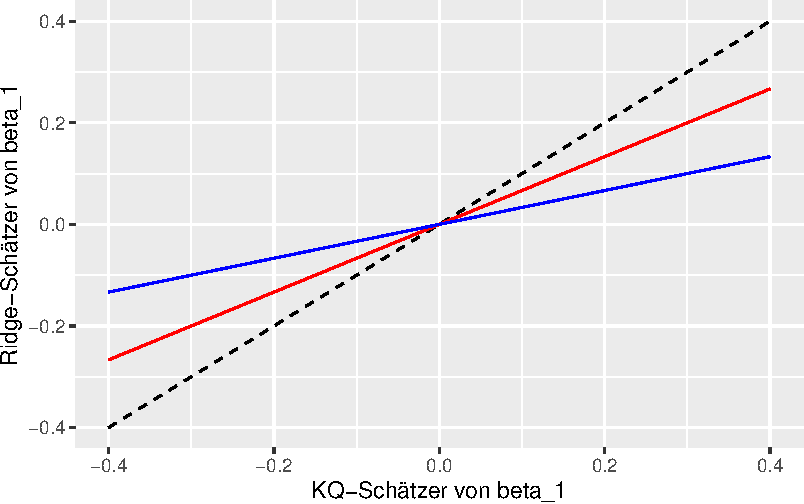
\includegraphics{RegReg_files/figure-pdf/fig-ridgeortho-1.pdf}

}

\caption{\label{fig-ridgeortho}Shrinkage des OLS-Schätzers bei Ridge
Regression}

\end{figure}

Abbildung~\ref{fig-ridgeortho} zeigt, dass der Ridge-Schätzer eine
lineare Transformation des KQ-Schätzers (gestrichelte Linie) ist.
Größere Werte des Regularisierungsparameters \(\lambda\) führen zu
stärkerer Shrinkage des Koeffizientenschätzers in Richtung 0. Die
\(\ell_2\)-Norm führt zu proportional zum Absolutwert des KQ-Schätzers
verlaufender Shrinkage: Größere Koeffizienten werden stärker bestraft
als kleine Koeffizienten.

Die Eigenschaft
\[\mathrm{E}\left(\widehat{\boldsymbol{\beta}}^{\mathrm{R}}_{\lambda,\,j}\right) = (1+\lambda)^{-1} \cdot \beta_j\]
zeigt, dass \(\widehat{\boldsymbol{\beta}}^{\mathrm{R}}_{\lambda,\,j}\)
(für fixes \(\lambda>0\)) nicht erwartungstreu für \(\beta_j\) ist.
Weiterhin ist \begin{align*}
  \mathrm{Var}\left(\widehat{\beta}^{\mathrm{R}}_{\lambda,\,j}\right) =&\, 
  \mathrm{Var}\left(\widehat{\beta}_j\right) \cdot \left(\frac{\lambda}{1+\lambda^2}\right)\\
    =&\, \sigma^2\cdot \left(\frac{\lambda}{1+\lambda^2}\right),
\end{align*} wobei \(\sigma^2\) die Varianz des Regressionsfehlers \(u\)
ist. Wegen \(\lambda<(1+\lambda)^2\) für \(\lambda>0\) gilt
\[\mathrm{Var}\left(\widehat{\beta}^{\mathrm{R}}_{\lambda,\,j}\right)<\mathrm{Var}\left(\widehat{\beta}_j\right).\]
Der Ridge-Schätzer hat also eine kleinere Varianz als der KQ-Schätzer.
Diese Eigenschaften können auch für korrelierte Regressoren gezeigt
werden.

\hypertarget{ridge-regression-mit-glmnet}{%
\subsection{\texorpdfstring{Ridge Regression mit
\texttt{glmnet}}{Ridge Regression mit glmnet}}\label{ridge-regression-mit-glmnet}}

Wir zeigen nun anhand simulierter Daten, wie der Ridge-Lösungspfad mit
dem R-Paket \texttt{glmnet} berechnet werden kann. Wir erzeugen zunächst
Daten gemäß der Vorschrift \begin{align}
  \begin{split}
  Y_i =&\, \boldsymbol{X}_i' \boldsymbol{\beta} + u_i,\\
  \\
  \beta_j =&\,  \frac{5}{j^2}, \qquad\qquad\ j=1,\dots,5,\\ 
  \beta_j =&\, -\frac{5}{(j-5)^2}, \quad j=6,\dots,10,\\
  \\
  \boldsymbol{X}_i \sim&\, N(\boldsymbol{0}, \boldsymbol{\Sigma}), \quad u_i \overset{u.i.v.}{\sim} N(0, 1), \quad i = 1,\dots,25.
  \end{split} \label{eq:ridgedgp1}
\end{align} Hierbei wird \(\boldsymbol{\Sigma}\) so definiert, dass
jeder Regressor \(N(0,1)\)-verteilt ist und eine Korrelation von \(0.8\)
mit allen anderen Regressoren aufweist. Mit der Vorschrift für die
\(\beta_j\) stellen wir sicher, dass es wenige Variablen gibt, die \(Y\)
stark beeinflussen, da der Absolutbetrag der Koeffizienten in \(j\)
abnimmt.\footnote{Für bessere Interpretierbarkeit der Grafischen
  Auswertung, wählen wir positive und negative Koeffizienten mit
  gleichem Bertag.}

\begin{Shaded}
\begin{Highlighting}[]
\FunctionTok{library}\NormalTok{(gendata)}
\FunctionTok{set.seed}\NormalTok{(}\DecValTok{1234}\NormalTok{)}

\CommentTok{\# Parameter definieren}
\NormalTok{N }\OtherTok{\textless{}{-}} \DecValTok{80}
\NormalTok{k }\OtherTok{\textless{}{-}} \DecValTok{10}

\NormalTok{coefs }\OtherTok{\textless{}{-}} \DecValTok{5}\SpecialCharTok{/}\NormalTok{(}\DecValTok{1}\SpecialCharTok{:}\NormalTok{(k}\SpecialCharTok{/}\DecValTok{2}\NormalTok{))}\SpecialCharTok{\^{}}\DecValTok{2}
\NormalTok{beta }\OtherTok{\textless{}{-}} \FunctionTok{c}\NormalTok{(coefs, }\SpecialCharTok{{-}}\NormalTok{coefs)}

\CommentTok{\# Beobachtungen simulieren}
\NormalTok{X }\OtherTok{\textless{}{-}} \FunctionTok{as.matrix}\NormalTok{(}
  \FunctionTok{genmvnorm}\NormalTok{(}
    \AttributeTok{k =}\NormalTok{ k, }
    \AttributeTok{cor =} \FunctionTok{rep}\NormalTok{(.}\DecValTok{8}\NormalTok{, (k}\SpecialCharTok{\^{}}\DecValTok{2}\SpecialCharTok{{-}}\NormalTok{k)}\SpecialCharTok{/}\DecValTok{2}\NormalTok{), }
    \AttributeTok{n =}\NormalTok{ N)}
\NormalTok{  )}
\NormalTok{Y }\OtherTok{\textless{}{-}}\NormalTok{ X }\SpecialCharTok{\%*\%}\NormalTok{ beta }\SpecialCharTok{+} \FunctionTok{rnorm}\NormalTok{(N)}
\end{Highlighting}
\end{Shaded}

Wir schätzen nun ein Modell mit allen 10 Regressoren mit
\texttt{glmnet}. Beachte, dass für den Ridge-Strafterm
\texttt{alpha\ =\ 0} gesetzt werden muss.\footnote{\texttt{alpha} ist
  ein Mischparameter im Algorithmus für
  \href{https://en.wikipedia.org/wiki/Elastic_net_regularization}{elastic
  net}, siehe \texttt{?glmnet}.}

\begin{Shaded}
\begin{Highlighting}[]
\FunctionTok{library}\NormalTok{(glmnet)}

\CommentTok{\# Ridge{-}Regression anpassen}
\NormalTok{ridge\_fit }\OtherTok{\textless{}{-}} \FunctionTok{glmnet}\NormalTok{(}
  \AttributeTok{x =}\NormalTok{ X, }
  \AttributeTok{y =}\NormalTok{ Y, }
  \AttributeTok{alpha =} \DecValTok{0} \CommentTok{\# für Ridge{-}Strafterm}
\NormalTok{)}
\end{Highlighting}
\end{Shaded}

Der Lösungspfad der Ridge-Schätzung kann nach Transformation der
geschätzen Koeffizienten und der zugehörigen \(\lambda\)-Werte in ein
langes Format überführt und komfortabel mit \texttt{ggplot2} dargestellt
werden.

\begin{Shaded}
\begin{Highlighting}[]
\CommentTok{\# Lambda{-}Sequenz auslesen}
\NormalTok{lambdas }\OtherTok{\textless{}{-}}\NormalTok{ ridge\_fit}\SpecialCharTok{$}\NormalTok{lambda}

\CommentTok{\# Ridge{-}Schätzung für Lambdas im langen Format }
\FunctionTok{as.matrix}\NormalTok{(ridge\_fit}\SpecialCharTok{$}\NormalTok{beta) }\SpecialCharTok{\%\textgreater{}\%} 
  \FunctionTok{as\_tibble}\NormalTok{() }\SpecialCharTok{\%\textgreater{}\%} 
  \FunctionTok{rownames\_to\_column}\NormalTok{(}\StringTok{"Variable"}\NormalTok{) }\SpecialCharTok{\%\textgreater{}\%}
  \FunctionTok{pivot\_longer}\NormalTok{(}\SpecialCharTok{{-}}\NormalTok{Variable) }\SpecialCharTok{\%\textgreater{}\%} 
  \FunctionTok{group\_by}\NormalTok{(Variable) }\SpecialCharTok{\%\textgreater{}\%} 
  \FunctionTok{mutate}\NormalTok{(}\AttributeTok{lambda =}\NormalTok{ lambdas) }\SpecialCharTok{\%\textgreater{}\%}
  
  \CommentTok{\# Grafik mit ggplot erzeugen}
  \FunctionTok{ggplot}\NormalTok{(}
    \AttributeTok{mapping =} \FunctionTok{aes}\NormalTok{(}
      \AttributeTok{x =}\NormalTok{ lambda, }
      \AttributeTok{y =}\NormalTok{ value, }
      \AttributeTok{col =}\NormalTok{ Variable}
\NormalTok{    )}
\NormalTok{  ) }\SpecialCharTok{+} 
  \FunctionTok{geom\_line}\NormalTok{() }\SpecialCharTok{+}
  \FunctionTok{ylab}\NormalTok{(}\StringTok{"gesch. Koeffizienten"}\NormalTok{) }\SpecialCharTok{+}
  \FunctionTok{scale\_x\_log10}\NormalTok{(}\StringTok{"log\_10(lambda)"}\NormalTok{)}
\end{Highlighting}
\end{Shaded}

\begin{figure}[t]

{\centering 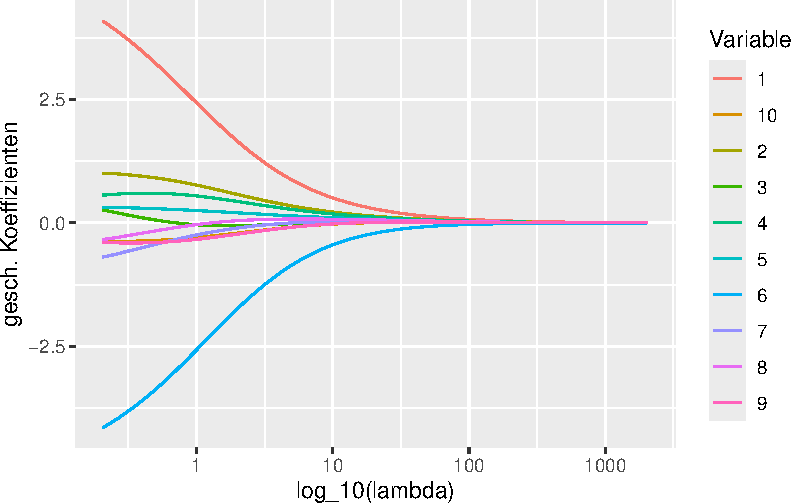
\includegraphics{RegReg_files/figure-pdf/fig-ridgesolpath-1.pdf}

}

\caption{\label{fig-ridgesolpath}Lösungspfad für Ridge-Schätzung}

\end{figure}

Abbildung~\ref{fig-ridgesolpath} zeigt den nicht-linearen Verlauf der
Shrinkage auf den geschätzten Modellkoeffizienten. Die Koeffizienten
werden mit zunehmendem \(\lambda\) von der KQ-Lösung ausgehend (linkes
Ende der Skala) in Richtung 0 gezwungen.

Über die Funktion \texttt{cv.glmnet()} kann ein optimales \(\lambda\)
mit Cross Validation (CV) ermittelt werden. Ähnlich wie bei
\texttt{glmnet()} wird für die Validierung automatisch eine
\(\lambda\)-Sequenz erzeugt. Wir nutzen \texttt{autoplot()} aus dem
R-Paket \texttt{ggfortify} für die Visualisierung der Ergebnisse mit
\texttt{ggplot2}.

\begin{Shaded}
\begin{Highlighting}[]
\FunctionTok{library}\NormalTok{(ggfortify)}

\CommentTok{\# Cross{-}validierte Bestimmung von lambda}
\NormalTok{ridge\_cvfit }\OtherTok{\textless{}{-}} \FunctionTok{cv.glmnet}\NormalTok{(}
  \AttributeTok{y =}\NormalTok{ Y, }
  \AttributeTok{x =}\NormalTok{ X, }
  \AttributeTok{intercept =}\NormalTok{ F,}
  \AttributeTok{alpha =} \DecValTok{0}
\NormalTok{) }

\CommentTok{\# Ergebnisse plotten}
\NormalTok{ridge\_cvfit }\SpecialCharTok{\%\textgreater{}\%} 
  \FunctionTok{autoplot}\NormalTok{(}\AttributeTok{label.n =} \DecValTok{0}\NormalTok{)}
\end{Highlighting}
\end{Shaded}

\begin{figure}[t]

{\centering 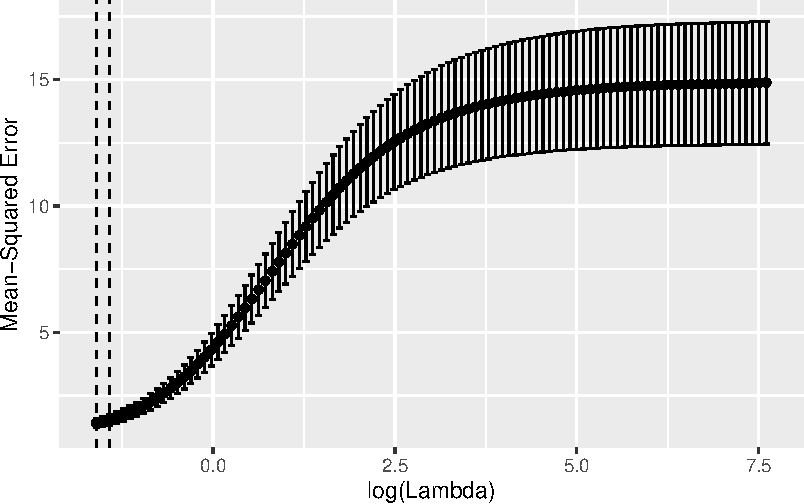
\includegraphics{RegReg_files/figure-pdf/fig-ridgecvplot-1.pdf}

}

\caption{\label{fig-ridgecvplot}Lösungspfad für Ridge-Schätzung}

\end{figure}

Abbildung~\ref{fig-ridgecvplot} zeigt \texttt{ridge\_cvfit\$lambda.min},
das optimale \(\lambda\) mit dem geringsten CV Mean-Squarred-Error
(linke gestrichelte Linie) und \texttt{ridge\_cvfit\$lambda.1se}, das
größte \(\lambda\), welches innerhalb einer Standardabweichung entfernt
ist (rechte gestrichelte Linie).\footnote{Die Wahl von
  \texttt{lambda.1se} ist eine Heuristik, welche die Schätzunsicherheit
  berücksichtigt und zu einem ``sparsameren'' Modell tendiert.} Wir
berechnen die Schätzung für \texttt{lambda.min}.

\begin{Shaded}
\begin{Highlighting}[]
\NormalTok{(}
\NormalTok{  ridge\_coefs }\OtherTok{\textless{}{-}} \FunctionTok{coef}\NormalTok{(}
    \AttributeTok{object =}\NormalTok{ ridge\_cvfit, }
    \AttributeTok{s =}\NormalTok{ ridge\_cvfit}\SpecialCharTok{$}\NormalTok{lambda.min}
\NormalTok{  )}
\NormalTok{)}
\end{Highlighting}
\end{Shaded}

\begin{verbatim}
11 x 1 sparse Matrix of class "dgCMatrix"
                    s1
(Intercept)  .        
X1           4.1302194
X2           1.0245661
X3           0.3139297
X4           0.5697498
X5           0.2928664
X6          -4.1693524
X7          -0.7509305
X8          -0.3844761
X9          -0.3841997
X10         -0.4078514
\end{verbatim}

Wir schätzen das Modell nun mit KQ und vergleichen die Koeffizienten mit
der Ridge-Schätzung.

\begin{Shaded}
\begin{Highlighting}[]
\CommentTok{\# KQ{-}Schätzung durchführen}
\NormalTok{KQ\_fit }\OtherTok{\textless{}{-}} \FunctionTok{lm}\NormalTok{(Y }\SpecialCharTok{\textasciitilde{}}\NormalTok{ X }\SpecialCharTok{{-}} \DecValTok{1}\NormalTok{)}

\CommentTok{\# Koeffizienten auslesen und transformieren:}
\FunctionTok{tibble}\NormalTok{(}
  \AttributeTok{Ridge =} \FunctionTok{as.matrix}\NormalTok{(ridge\_coefs)[}\DecValTok{2}\SpecialCharTok{:}\DecValTok{11}\NormalTok{, ],}
  \AttributeTok{KQ =}\NormalTok{ KQ\_fit}\SpecialCharTok{$}\NormalTok{coefficients}
\NormalTok{) }\SpecialCharTok{\%\textgreater{}\%} 
  \FunctionTok{mutate}\NormalTok{(}\AttributeTok{j =} \FunctionTok{factor}\NormalTok{(}\DecValTok{1}\SpecialCharTok{:}\DecValTok{10}\NormalTok{)) }\SpecialCharTok{\%\textgreater{}\%}
  \FunctionTok{pivot\_longer}\NormalTok{(}
    \AttributeTok{cols =}\NormalTok{ Ridge}\SpecialCharTok{:}\NormalTok{KQ, }
    \AttributeTok{names\_to =} \StringTok{"Methode"}\NormalTok{, }
    \AttributeTok{values\_to =} \StringTok{"Koeffizient"}
\NormalTok{  ) }\SpecialCharTok{\%\textgreater{}\%}

\CommentTok{\# Bar{-}Plot für Koeffizientenvergleich erzeugen  }
  \FunctionTok{ggplot}\NormalTok{(}
    \AttributeTok{mapping =} \FunctionTok{aes}\NormalTok{(}
      \AttributeTok{x =}\NormalTok{ j, }
      \AttributeTok{y =}\NormalTok{ Koeffizient, }
      \AttributeTok{fill =}\NormalTok{ Methode}
\NormalTok{    )}
\NormalTok{  ) }\SpecialCharTok{+}
  \FunctionTok{geom\_bar}\NormalTok{(}
    \AttributeTok{position =} \StringTok{"dodge"}\NormalTok{, }
    \AttributeTok{stat =} \StringTok{"identity"}\NormalTok{, }
    \AttributeTok{width =}\NormalTok{ .}\DecValTok{5}
\NormalTok{  )}
\end{Highlighting}
\end{Shaded}

\begin{figure}[t]

{\centering 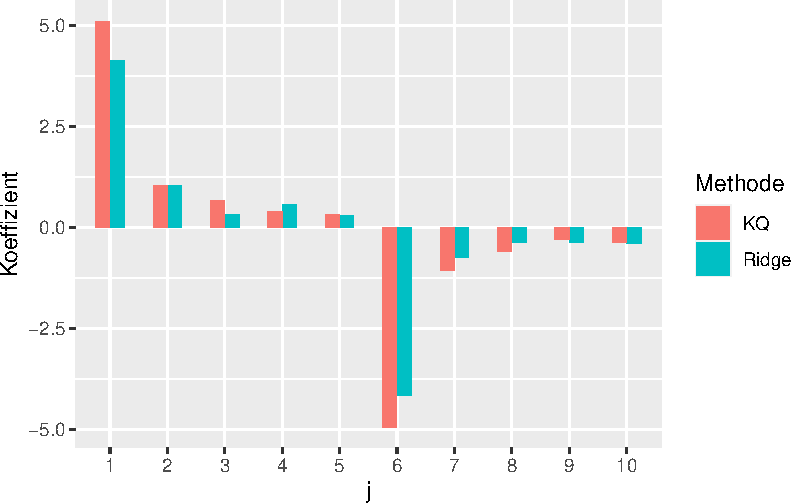
\includegraphics{RegReg_files/figure-pdf/fig-KoefRidgeVsKQ-1.pdf}

}

\caption{\label{fig-KoefRidgeVsKQ}Koeffizientenvergleich: Ridge vs.~KQ}

\end{figure}

Der Vergleich anhand von Abbildung~\ref{fig-KoefRidgeVsKQ} zeigt
deutlich, dass Ridge Regression im Vergleich mit KQ zu absolut kleineren
Koeffizientenschätzungen tendiert. Inwiefern dies Konsequenzen für die
Prognosegüte der Schätzung hat, können wir Anhand eines Testdatensatzes
bestimmen. Hierzu vergleichen wir die mittleren Fehler (MSE) bei der
Prognose von \(Y\) für die Beobachtungen im Testdatensatz. Für die
Simulation des Testdatensatzes nutzen wir erneut die Vorschrift
\eqref{eq:ridgedgp1} um 80 neue Beobachtungen zu erzeugen.

\begin{Shaded}
\begin{Highlighting}[]
\CommentTok{\# Test{-}Datensatz erstellen}
\FunctionTok{set.seed}\NormalTok{(}\DecValTok{4321}\NormalTok{)}
\CommentTok{\# Regressoren}
\NormalTok{new\_X }\OtherTok{\textless{}{-}} \FunctionTok{as.matrix}\NormalTok{(}
  \FunctionTok{genmvnorm}\NormalTok{(}
    \AttributeTok{k =}\NormalTok{ k, }
    \AttributeTok{cor =} \FunctionTok{rep}\NormalTok{(.}\DecValTok{85}\NormalTok{, (k}\SpecialCharTok{\^{}}\DecValTok{2}\SpecialCharTok{{-}}\NormalTok{k)}\SpecialCharTok{/}\DecValTok{2}\NormalTok{), }
    \AttributeTok{n =}\NormalTok{ N}
\NormalTok{  )}
\NormalTok{)}
\CommentTok{\# Abh. Variable}
\NormalTok{new\_Y }\OtherTok{\textless{}{-}}\NormalTok{ new\_X }\SpecialCharTok{\%*\%}\NormalTok{ beta }\SpecialCharTok{+} \FunctionTok{rnorm}\NormalTok{(N)}
\end{Highlighting}
\end{Shaded}

Für beide Methoden können wir \texttt{predict()} für die Prognosen von
\(Y\) für den Testdatensatz (\texttt{new\_Y}) nutzen.

\begin{Shaded}
\begin{Highlighting}[]
\CommentTok{\# Ridge: Vorhersage von new\_Y für Test{-}Datensatz}
\NormalTok{Y\_predict\_ridge }\OtherTok{\textless{}{-}} \FunctionTok{predict}\NormalTok{(}
  \AttributeTok{object =}\NormalTok{ ridge\_cvfit, }
  \AttributeTok{newx =}\NormalTok{ new\_X, }
  \AttributeTok{s =}\NormalTok{ ridge\_cvfit}\SpecialCharTok{$}\NormalTok{lambda.min}
\NormalTok{)}

\CommentTok{\# Ridge: MSE für Test{-}Datensatz berechnen}
\FunctionTok{mean}\NormalTok{((Y\_predict\_ridge }\SpecialCharTok{{-}}\NormalTok{ new\_Y)}\SpecialCharTok{\^{}}\DecValTok{2}\NormalTok{)}
\end{Highlighting}
\end{Shaded}

\begin{verbatim}
[1] 1.288457
\end{verbatim}

Die Vorhersage für \texttt{lm()} benötigt dieselben Variablennamen wie
im angepassten Modell, s. \texttt{KQ\_fit\$coefficients}.

\begin{Shaded}
\begin{Highlighting}[]
\CommentTok{\# Test{-}Datensatz für predict.lm() formatieren}
\NormalTok{new\_X }\OtherTok{\textless{}{-}} \FunctionTok{as.data.frame}\NormalTok{(new\_X)}
\FunctionTok{colnames}\NormalTok{(new\_X) }\OtherTok{\textless{}{-}} \FunctionTok{paste0}\NormalTok{(}\StringTok{"X"}\NormalTok{, }\DecValTok{1}\SpecialCharTok{:}\NormalTok{k)}

\CommentTok{\# KQ: Vorhersage von new\_Y für Test{-}Datensatz}
\NormalTok{Y\_predict\_KQ }\OtherTok{\textless{}{-}} \FunctionTok{predict}\NormalTok{(}
  \AttributeTok{object =}\NormalTok{ KQ\_fit, }
  \AttributeTok{newdata =}\NormalTok{ new\_X}
\NormalTok{)}

\CommentTok{\# KQ: MSE für Test{-}Datensatz berechnen}
\FunctionTok{mean}\NormalTok{((Y\_predict\_KQ }\SpecialCharTok{{-}}\NormalTok{ new\_Y)}\SpecialCharTok{\^{}}\DecValTok{2}\NormalTok{)}
\end{Highlighting}
\end{Shaded}

\begin{verbatim}
[1] 29.33797
\end{verbatim}

Die Ergebnisse zeigen, dass der Ridge-Schätzer trotz seiner Verzerrung
einen deutlich geringeren mittleren Vorhersagefehler für die Testdaten
erzielt als der KQ-Schätzer. Diese Eigenschaft der
Koeffizientenschätzung kann die Prognosegüte von Ridge Regression
gegenüber der KQ-Regression verbessern.

\hypertarget{beispiel-vorhersage-von-abschlussnoten-in-mathe}{%
\subsection{Beispiel: Vorhersage von Abschlussnoten in
Mathe}\label{beispiel-vorhersage-von-abschlussnoten-in-mathe}}

Zur Illustration von Ridge Regression nutzen wir den Datensatz
\texttt{SP} aus Cortez und Silva (2008).\footnote{Wir verwenden eine
  Auszug aus dem Orignaldatensatz, der nebst ausführlicher
  Variablenbeschreibung
  \href{https://archive.ics.uci.edu/dataset/320/student+performance}{hier}
  verfügbar ist.} \texttt{SP} enhält Beobachtungen zu Leistungen von
insgesamt 100 Schülerinnen und Schülern im Fach Mathematik in der
Sekundarstufe an zwei portugiesischen Schulen. Neben der Abschlussnote
in Mathe (\texttt{G3}, Skala von 0 bis 20) beinhaltet \texttt{SP}
diverse demografische, soziale und schulbezogene Merkmale, die mithilfe
von Schulberichten und Fragebögen erhoben wurden. Ziel ist es, ein
Modell für die Prognose von \texttt{G3} anzupassen.

Wir lesen zunächst die Daten (im .csv-Format) ein.

\begin{Shaded}
\begin{Highlighting}[]
\CommentTok{\# Daten einlesen}
\NormalTok{SP }\OtherTok{\textless{}{-}} \FunctionTok{read\_csv}\NormalTok{(}\AttributeTok{file =} \StringTok{"datasets/SP.csv"}\NormalTok{)}
\end{Highlighting}
\end{Shaded}

Ein Überblick zeigt, dass der Großteil der Regressoren aus kategorialen
Variablen mit sozio-ökonomischen Informationen besteht.

\begin{Shaded}
\begin{Highlighting}[]
\CommentTok{\# Überblick}
\FunctionTok{glimpse}\NormalTok{(SP)}
\end{Highlighting}
\end{Shaded}

\begin{verbatim}
Rows: 100
Columns: 31
$ school     <chr> "GP", "GP", "GP", "MS", "GP", "GP", "GP", "GP", "GP", "GP",~
$ sex        <chr> "M", "M", "F", "F", "M", "F", "F", "F", "F", "F", "M", "M",~
$ age        <dbl> 17, 18, 19, 17, 16, 16, 19, 16, 16, 16, 18, 16, 15, 17, 17,~
$ address    <chr> "R", "R", "U", "U", "U", "U", "U", "U", "U", "R", "U", "U",~
$ famsize    <chr> "GT3", "GT3", "LE3", "GT3", "LE3", "GT3", "GT3", "GT3", "GT~
$ Pstatus    <chr> "T", "T", "T", "T", "A", "T", "T", "T", "A", "T", "T", "T",~
$ Medu       <dbl> 1, 4, 3, 2, 3, 2, 0, 2, 3, 4, 4, 2, 1, 2, 2, 3, 3, 4, 4, 2,~
$ Fedu       <dbl> 2, 3, 2, 2, 4, 3, 1, 1, 1, 4, 4, 2, 2, 3, 2, 3, 1, 3, 4, 2,~
$ Mjob       <chr> "at_home", "teacher", "services", "other", "services", "oth~
$ Fjob       <chr> "other", "services", "other", "at_home", "other", "other", ~
$ reason     <chr> "home", "course", "reputation", "home", "home", "reputation~
$ guardian   <chr> "mother", "mother", "other", "mother", "mother", "mother", ~
$ traveltime <dbl> 1, 1, 2, 1, 1, 1, 1, 1, 1, 1, 1, 2, 1, 1, 1, 2, 1, 1, 1, 1,~
$ studytime  <dbl> 2, 3, 2, 3, 2, 2, 2, 1, 2, 2, 1, 2, 2, 2, 1, 1, 2, 3, 1, 2,~
$ failures   <dbl> 0, 0, 1, 0, 0, 0, 3, 0, 3, 0, 0, 0, 0, 0, 0, 0, 0, 0, 0, 0,~
$ schoolsup  <chr> "no", "no", "no", "no", "yes", "yes", "no", "no", "no", "no~
$ famsup     <chr> "no", "no", "yes", "no", "yes", "yes", "yes", "no", "yes", ~
$ paid       <chr> "no", "no", "yes", "no", "no", "yes", "no", "no", "yes", "n~
$ activities <chr> "no", "no", "no", "yes", "yes", "yes", "no", "no", "no", "y~
$ nursery    <chr> "yes", "yes", "no", "yes", "yes", "yes", "no", "yes", "yes"~
$ higher     <chr> "yes", "yes", "yes", "yes", "yes", "yes", "no", "yes", "yes~
$ internet   <chr> "no", "yes", "yes", "no", "yes", "no", "no", "yes", "yes", ~
$ romantic   <chr> "no", "yes", "yes", "yes", "no", "no", "no", "yes", "no", "~
$ famrel     <dbl> 3, 5, 4, 3, 5, 4, 3, 4, 2, 2, 1, 5, 4, 5, 3, 5, 4, 4, 5, 5,~
$ freetime   <dbl> 1, 3, 2, 4, 3, 4, 4, 5, 3, 4, 4, 4, 3, 3, 4, 4, 5, 2, 3, 4,~
$ goout      <dbl> 3, 2, 2, 3, 3, 3, 2, 2, 3, 4, 2, 4, 2, 3, 4, 2, 4, 2, 3, 4,~
$ Dalc       <dbl> 1, 1, 1, 1, 1, 1, 1, 1, 2, 2, 2, 2, 1, 1, 1, 1, 2, 1, 1, 1,~
$ Walc       <dbl> 5, 2, 2, 1, 1, 3, 1, 1, 2, 3, 2, 4, 1, 3, 3, 1, 3, 2, 1, 1,~
$ health     <dbl> 3, 4, 1, 3, 5, 4, 5, 5, 4, 4, 1, 5, 5, 3, 5, 5, 1, 3, 5, 5,~
$ absences   <dbl> 4, 9, 22, 8, 4, 6, 2, 20, 5, 6, 5, 0, 2, 2, 12, 0, 17, 0, 4~
$ G3         <dbl> 10, 16, 11, 11, 11, 10, 9, 12, 7, 11, 16, 12, 9, 12, 12, 13~
\end{verbatim}

Um die Prognosegüte des Modells beurteilen zu können, partitionieren wir
\texttt{SP} zufällig in einen Test- sowie einen Trainingsdatensatz (mit
30 und 70 Beobachtungen), jeweils für die Regressoren und die abhängige
Variable.

\begin{Shaded}
\begin{Highlighting}[]
\CommentTok{\# ID für Beobachtungen im Testdatensatz zufällig erzeugen}
\FunctionTok{set.seed}\NormalTok{(}\DecValTok{1234}\NormalTok{)}
\NormalTok{ID }\OtherTok{\textless{}{-}} \FunctionTok{sample}\NormalTok{(}\DecValTok{1}\SpecialCharTok{:}\FunctionTok{nrow}\NormalTok{(SP), }\AttributeTok{size =} \DecValTok{30}\NormalTok{)}

\CommentTok{\# Regressoren aufteilen}
\NormalTok{SP\_test }\OtherTok{\textless{}{-}}\NormalTok{ SP[ID,]}
\NormalTok{SP\_train }\OtherTok{\textless{}{-}}\NormalTok{ SP[}\SpecialCharTok{{-}}\NormalTok{ID,]}

\CommentTok{\# Abh. Variable aufteilen}
\NormalTok{Y\_test }\OtherTok{\textless{}{-}}\NormalTok{ SP\_test}\SpecialCharTok{$}\NormalTok{G3}
\NormalTok{Y\_train }\OtherTok{\textless{}{-}}\NormalTok{ SP\_train}\SpecialCharTok{$}\NormalTok{G3}
\end{Highlighting}
\end{Shaded}

Als nächstes passen wir ein Ridge-Regressionsmodell für alle Regressoren
in \texttt{SP\_train} an und ermitteln ein optimales \(\lambda\) mit
Cross Validation. Beachte, dass \texttt{cv.glmnet} nicht für Regressoren
im \texttt{data.frame}/\texttt{tibble}-Format ausgelegt ist, sondern ein
\texttt{matrix}-Format erwartet. Wir transformieren \texttt{SP\_train}
daher mit \texttt{data.matrix()}.

\begin{Shaded}
\begin{Highlighting}[]
\CommentTok{\# Ridge{-}Regression und CV für Trainingsdaten}
\NormalTok{SP\_fit\_cv }\OtherTok{\textless{}{-}} \FunctionTok{cv.glmnet}\NormalTok{(}
  \AttributeTok{x =} \FunctionTok{data.matrix}\NormalTok{(SP\_train }\SpecialCharTok{\%\textgreater{}\%} \FunctionTok{select}\NormalTok{(}\SpecialCharTok{{-}}\NormalTok{G3)), }
  \AttributeTok{y =}\NormalTok{ Y\_train, }
  \AttributeTok{alpha =} \DecValTok{0}
\NormalTok{)}

\CommentTok{\# CV{-}Ergebnisse für lambda visualisieren}
\NormalTok{SP\_fit\_cv }\SpecialCharTok{\%\textgreater{}\%} 
  \FunctionTok{autoplot}\NormalTok{(}\AttributeTok{label.n =} \DecValTok{0}\NormalTok{)}
\end{Highlighting}
\end{Shaded}

\begin{figure}[t]

{\centering 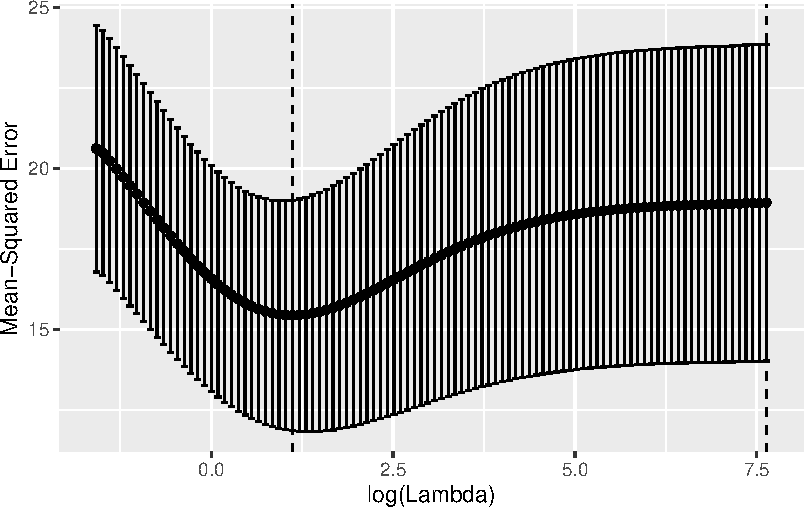
\includegraphics{RegReg_files/figure-pdf/unnamed-chunk-16-1.pdf}

}

\end{figure}

Wie für das Beispiel mit simulierten Daten erhalten wir mit
\texttt{predict()} Vorhersagen für die erzielte Punktzahl. Beachte, dass
wir den MSE nicht für die Trainingsdaten \texttt{SP\_train}, sondern für
die Testdaten \texttt{SP\_test} berechnen.

\begin{Shaded}
\begin{Highlighting}[]
\CommentTok{\# Prognose von G3 anhand des Ridge{-}Modells}
\NormalTok{Y\_predict\_ridge }\OtherTok{\textless{}{-}} \FunctionTok{predict}\NormalTok{(}
  \AttributeTok{object =}\NormalTok{ SP\_fit\_cv, }
  \AttributeTok{newx =} \FunctionTok{data.matrix}\NormalTok{(}
\NormalTok{    SP\_test }\SpecialCharTok{\%\textgreater{}\%} 
      \FunctionTok{select}\NormalTok{(}\SpecialCharTok{{-}}\NormalTok{G3)}
\NormalTok{    ), }
  \AttributeTok{s =}\NormalTok{ SP\_fit\_cv}\SpecialCharTok{$}\NormalTok{lambda.min}
\NormalTok{)}

\CommentTok{\# MSE für Testdaten berechnen}
\FunctionTok{mean}\NormalTok{((Y\_predict\_ridge }\SpecialCharTok{{-}}\NormalTok{ Y\_test)}\SpecialCharTok{\^{}}\DecValTok{2}\NormalTok{)}
\end{Highlighting}
\end{Shaded}

\begin{verbatim}
[1] 21.13249
\end{verbatim}

Auch in diesem empirischen Beispiel zeigt ein Vergleich der MSEs, dass
Ridge Regression dem KQ-Schätzer hinsichtlich der Vorhersagegüte
überlegen ist.

\begin{Shaded}
\begin{Highlighting}[]
\CommentTok{\# Modell mit KQ schätzen}
\NormalTok{SP\_fit\_KQ }\OtherTok{\textless{}{-}} \FunctionTok{lm}\NormalTok{(G3 }\SpecialCharTok{\textasciitilde{}}\NormalTok{ ., SP\_train)}

\CommentTok{\# Prognose}
\NormalTok{Y\_predict\_KQ }\OtherTok{\textless{}{-}} \FunctionTok{predict}\NormalTok{(}
  \AttributeTok{object =}\NormalTok{ SP\_fit\_KQ, }
  \AttributeTok{newdata =}\NormalTok{ SP\_test }\SpecialCharTok{\%\textgreater{}\%} 
    \FunctionTok{select}\NormalTok{(}\SpecialCharTok{{-}}\NormalTok{G3)}
\NormalTok{)}

\CommentTok{\# Testset{-}MSE berechnen}
\FunctionTok{mean}\NormalTok{((Y\_predict\_KQ }\SpecialCharTok{{-}}\NormalTok{ Y\_test)}\SpecialCharTok{\^{}}\DecValTok{2}\NormalTok{)}
\end{Highlighting}
\end{Shaded}

\begin{verbatim}
[1] 29.76893
\end{verbatim}

Der MSE für Ridge ist mit \(21.13\) deutlich kleiner als \(29.77\), der
MSE für KQ.

Für die Interpretation der Ridge-Schätzung erweitern den Code für die
\texttt{ggplot2}-Grafik der Koeffizienten-Pfade um eine vertikale Linie
des mit CV ermittelten \(\lambda\) und fügen mit dem Paket
\texttt{ggrepel} Labels für die Pfade der größten Koeffizienten hinzu.

\begin{Shaded}
\begin{Highlighting}[]
\FunctionTok{library}\NormalTok{(ggrepel)}

\CommentTok{\# Lambda{-}Sequenz auslesen}
\NormalTok{lambdas }\OtherTok{\textless{}{-}}\NormalTok{ SP\_fit\_cv}\SpecialCharTok{$}\NormalTok{lambda}

\CommentTok{\# Ridge{-}Schätzung für Lambdas im langen Format }
\NormalTok{df }\OtherTok{\textless{}{-}} \FunctionTok{as.matrix}\NormalTok{(SP\_fit\_cv}\SpecialCharTok{$}\NormalTok{glmnet.fit}\SpecialCharTok{$}\NormalTok{beta) }\SpecialCharTok{\%\textgreater{}\%} 
  \FunctionTok{as\_tibble}\NormalTok{() }\SpecialCharTok{\%\textgreater{}\%} 
  \FunctionTok{mutate}\NormalTok{(}
    \AttributeTok{Variable =} \FunctionTok{rownames}\NormalTok{(SP\_fit\_cv}\SpecialCharTok{$}\NormalTok{glmnet.fit}\SpecialCharTok{$}\NormalTok{beta)}
\NormalTok{  ) }\SpecialCharTok{\%\textgreater{}\%}
  \FunctionTok{pivot\_longer}\NormalTok{(}\SpecialCharTok{{-}}\NormalTok{Variable) }\SpecialCharTok{\%\textgreater{}\%} 
  \FunctionTok{group\_by}\NormalTok{(Variable) }\SpecialCharTok{\%\textgreater{}\%} 
  \FunctionTok{mutate}\NormalTok{(}\AttributeTok{lambda =}\NormalTok{ lambdas) }

\CommentTok{\# Grafik mit ggplot erzeugen}
\NormalTok{df }\SpecialCharTok{\%\textgreater{}\%}
  \FunctionTok{ggplot}\NormalTok{(}
    \AttributeTok{mapping =} \FunctionTok{aes}\NormalTok{(}
      \AttributeTok{x =}\NormalTok{ lambda, }
      \AttributeTok{y =}\NormalTok{ value, }
      \AttributeTok{col =}\NormalTok{ Variable}
\NormalTok{    )}
\NormalTok{  ) }\SpecialCharTok{+} 
  \FunctionTok{geom\_line}\NormalTok{() }\SpecialCharTok{+}
  \FunctionTok{geom\_label\_repel}\NormalTok{(}
    \AttributeTok{data =}\NormalTok{ df }\SpecialCharTok{\%\textgreater{}\%} 
      \FunctionTok{filter}\NormalTok{(lambda }\SpecialCharTok{==} \FunctionTok{min}\NormalTok{(lambdas)),}
    \AttributeTok{mapping =} \FunctionTok{aes}\NormalTok{(}\AttributeTok{label =}\NormalTok{ Variable), }
    \AttributeTok{seed =} \DecValTok{1234}\NormalTok{,}
    \AttributeTok{size =} \DecValTok{5}\NormalTok{, }
    \AttributeTok{max.overlaps =} \DecValTok{8}\NormalTok{, }
    \AttributeTok{nudge\_x =} \SpecialCharTok{{-}}\NormalTok{.}\DecValTok{5}\NormalTok{) }\SpecialCharTok{+}
  \FunctionTok{ylab}\NormalTok{(}\StringTok{"gesch. Koeffizienten"}\NormalTok{) }\SpecialCharTok{+}
  \FunctionTok{scale\_x\_log10}\NormalTok{(}\StringTok{"log\_10(lambda)"}\NormalTok{) }\SpecialCharTok{+}
  \FunctionTok{geom\_vline}\NormalTok{(}
    \AttributeTok{xintercept =}\NormalTok{ SP\_fit\_cv}\SpecialCharTok{$}\NormalTok{lambda.min, }
    \AttributeTok{col =} \StringTok{"red"}\NormalTok{, }
    \AttributeTok{lty =} \DecValTok{2}
\NormalTok{  ) }\SpecialCharTok{+}
  \FunctionTok{theme}\NormalTok{(}\AttributeTok{legend.position =} \StringTok{"none"}\NormalTok{)}
\end{Highlighting}
\end{Shaded}

\begin{figure}[t]

{\centering 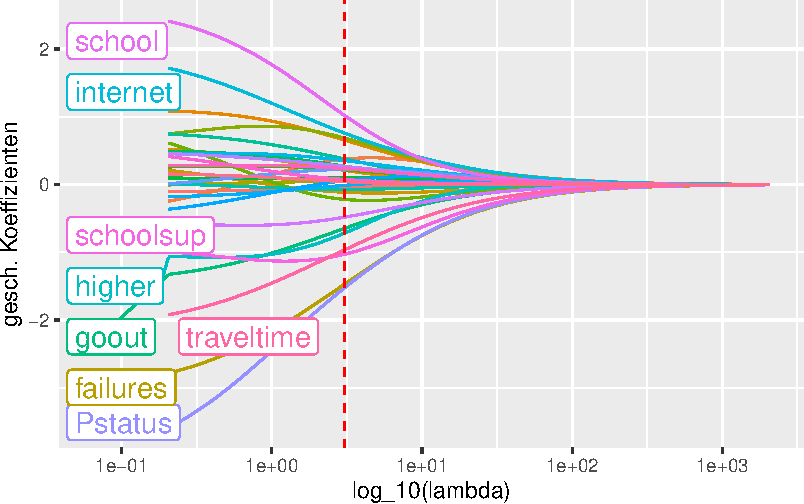
\includegraphics{RegReg_files/figure-pdf/fig-ridgAppPlot-1.pdf}

}

\caption{\label{fig-ridgAppPlot}Lösungspfad für Ridge-Schätzung}

\end{figure}

Abbildung~\ref{fig-ridgAppPlot} gibt Hinweise darauf, dass neben der
Schulzugehörigkeit und Indikatoren für schulische Leistung (bspw.
\texttt{failures}) sozio-ökonomische Prädiktoren wie \texttt{internet}
(Internetzugang zuhause), \texttt{Pstatus} (Zusammenleben der Eltern)
und \texttt{address}/\texttt{traveltime} (sozialer Status) relevante
Variablen zu sein scheinen.

Das optimale \(\lambda_\mathrm{cv} \approx 0.21\) (gestrichelte rote
Linie in Abbildung~\ref{fig-ridgAppPlot}) führt zu deutlicher Shrinkage,
was eine mögliche Erklärung für den besseren Testset-MSE von Ridge
Regression ist: Die Koeffizienten von Variablen mit wenig
Erklärungskraft werden durch die Regularisierung in Richtung 0 gezwungen
und reduzieren so die Varianz der Vorhersage gegenüber der
(idealerweise) unverzerrten KQ-Schätzung.

\begin{tcolorbox}[enhanced jigsaw, colbacktitle=quarto-callout-note-color!10!white, bottomtitle=1mm, breakable, leftrule=.75mm, opacityback=0, title=\textcolor{quarto-callout-note-color}{\faInfo}\hspace{0.5em}{Key Facts zu Ridge Regression}, left=2mm, arc=.35mm, titlerule=0mm, bottomrule=.15mm, opacitybacktitle=0.6, coltitle=black, toptitle=1mm, colback=white, colframe=quarto-callout-note-color-frame, toprule=.15mm, rightrule=.15mm]

\begin{itemize}
\item
  Ridge-Regression regularisiert den KQ-Schätzer mit der \(\ell_2\)-Norm
  der Koeffizienten. Diese Form von Regularisierung ist eine Alternative
  für KQ in Anwendungen mit mehr Regressoren als Beobachtugen
  (\(k\geq n\)) und/oder wenn KQ aufgrund starker Kollinearität eine
  hohe Varianz aufweist.
\item
  Der Ridge-Schätzer
  \(\widehat{\boldsymbol{\beta}}^{\mathrm{R}}_\lambda\) ist \emph{nicht}
  erwartungstreu. Die geschätzten Koeffizienten sind auch für
  \(n\to\infty\) verzerrt.
\item
  Aufgrund der verzerrten Schätzung ist statistische Inferenz für
  Koeffizienten mit
  \(\widehat{\boldsymbol{\beta}}^{\mathrm{R}}_\lambda\) problematisch.
  Anstatt für strukturelle Modelle oder die Schätzung kausaler Effekte
  wird Ridge Regression in der Praxis daher überwiegend für Prognosen
  verwendet.
\item
  Die Wahl von \(\lambda\) impliziert einen Tradeoff zwischen Verzerrung
  und Varianz: Große \(\lambda\) schrumpfen die Koeffizientenschätzer
  Richtung 0 (mehr Verzerrung), führen aber zu einer kleineren Varianz
  der Schätzung. Entsprechend können Vorhersagen mit mehr Verzerrung
  aber weniger Varianz als mit KQ getroffen werden.
\item
  Ridge Regression kann in R mit dem Paket \texttt{glmnet} berechnet
  werden.
\end{itemize}

\end{tcolorbox}

\hypertarget{lasso-regression}{%
\section{Lasso Regression}\label{lasso-regression}}

Least Absolute Shrinkage and Selection Operator (Lasso) ist ein von
Tibshirani (1996) vorgeschlagener Schätzer, der die Verlustfunktion des
KQ-Schätzers um einen Strafterm für die Summe der (absoluten) Größe der
Koeffizienten \(\boldsymbol\beta = (\beta_1, \dots,\beta_k)'\)
erweitert. Die Verlustfunktion des Lasso-Schätzers von
\(\boldsymbol{\beta}\) lautet \begin{align}
\mathrm{RSS}(\boldsymbol{\beta},p=1,\lambda) = \mathrm{RSS}(\boldsymbol{\beta}) + \lambda \lVert\boldsymbol{\beta}\rVert_1.\label{eq:lassoloss}
\end{align} Für den Strafterm wird also die \(\ell_1\)-norm \[
\lVert\boldsymbol{\beta}\rVert_1 = \sum_{j=1}^k \lvert\beta_j \rvert
\] verwendet. Der Lasso-Schätzer
\(\widehat{\boldsymbol{\beta}}^{\mathrm{L}}_\lambda\) für
\(\boldsymbol{\beta}\) minimiert \eqref{eq:lassoloss}, \begin{align}
\boldsymbol{\beta}^{\mathrm{L}}_\lambda = \arg\min_{\boldsymbol{\beta}} \ \mathrm{RSS}(\boldsymbol{\beta},p=1,\lambda).
\end{align} Entsprechend erhalten wir in Abhängigkeit von \(\lambda\)
ein Kontinuum an Lösungen \begin{align}
  \left\{\widehat{\boldsymbol{\beta}}^{\mathrm{L}}_\lambda\right\}_{\lambda=0}^{\lambda=\infty},\label{eq:LassoPath}
\end{align} der sogenannte \emph{Lasso-Pfad}.

Das Optimierungsproblem \eqref{eq:lassoloss} hat die äquivalente
Darstellung \begin{align}
  \begin{split}
    \widehat{\boldsymbol{\beta}}^{\mathrm{L}}_\lambda =&\, \arg\min_{\boldsymbol{\beta}} \mathrm{RSS}(\boldsymbol{\beta}) + \lambda\left(\lVert\boldsymbol{\beta}\rVert_1 - t\right)\\
    =&\, \arg\min_{\lVert\boldsymbol{\beta}\rVert_1\leq t} \mathrm{RSS}(\boldsymbol{\beta}), 
  \end{split}\label{eq:lassolagrange}
\end{align} welche über den
\href{https://de.wikipedia.org/wiki/Lagrange-Multiplikator\#Beispiel_mit_Anwendungsbezug}{Lagrange-Ansatz}
unter der Nebenbedingung \(\lVert\boldsymbol{\beta}\rVert_1 \leq t\)
gelöst werden kann.

Ähnlich wie der KQ-Schätzer ist der Lasso-Schätzer
\(\widehat{\boldsymbol{\beta}}^{\mathrm{L}}_\lambda\) durch Bedingungen
1. Ordnung bestimmt. Diese Bedingungen lassen sich komfortabel in
Matrix-Schreibweise darstellen als \begin{align}
  -2\boldsymbol{X}_j'(\boldsymbol{Y} - \boldsymbol{X}\boldsymbol{\beta}) + \lambda\cdot\mathrm{sgn}(\beta_j) = 0, \quad j = 1,\dots,k.\label{eq:LassoFOC}
\end{align} Aus Gleichung \eqref{eq:LassoFOC} folgt, dass der
Lasso-Schätzer aufgrund des Strafterms im Allgemeinen nicht algebraisch
bestimmt werden kann.\footnote{Zur Bestimmung des Schätzers werden
  Algorithmen der nicht-linearen Optimierung genutzt.}

In Abhängigkeit von \(\lambda\) zwingt der Lasso-Schätzer die
KQ-Schätzung von \(\beta_j\) zu einem (absolut) kleineren Wert: Ähnlich
wie bei Ridge Regression bewirkt der \(\ell_1\)-Strafterm eine mit
\(\lambda\) zunehmende Schrumpfung der geschätzen Koeffizienten in
Richtung 0. Charakteristisch für die Lösung des Lasso-Schätzers ist,
dass \(\widehat{\boldsymbol{\beta}}^{\mathrm{L}}_j = 0\), wenn die
Bedingung \begin{align}
  \left\lvert\boldsymbol{X}_j'(\boldsymbol{Y} - \boldsymbol{X}\widehat{\boldsymbol{\beta}}^{\mathrm{L}}_\lambda)\right\rvert - \lambda/2 \leq 0 \label{eq:lassoselection}
\end{align} erfüllt ist. In Abhängigkeit von \(\lambda\) kann der
Lasso-Schätzer folglich geschätzte Regressionskoeffizienten nicht nur in
Richtung \(0\), sondern diese auch \emph{exakt} mit \(0\) schätzen und
damit \emph{Variablenselektion} betreiben. Aufgrund der mit \(\lambda\)
zunehmenden Shrinkage bis die Bedingung \eqref{eq:lassoselection}
erfüllt und der Koeffizient gleich \(0\) gesetzt wird, bezeichnet man
Lasso auch als einen \emph{Soft Thresholding Operator}. Im nächsten
Abschnitt betrachten wir die Eigenschaften von Lasso-Regularisierung
unter vereinfachten Annahmen bzgl. der Regressoren.

\hypertarget{lasso-ist-soft-thresholding}{%
\subsection{Lasso ist Soft
Thresholding}\label{lasso-ist-soft-thresholding}}

Wir betrachten nun eine mathematische Darstellung von Selektions- und
Shrinkage-Eigenschaft des Lasso-Schätzers in einem vereinfachten Modell.
Wenn die Regressoren \(\boldsymbol{X}\) orthonormal zueinander sind,
existiert eine analytische Lösung des Lasso-Schätzers, \begin{align}
  \widehat{\boldsymbol{\beta}}^{\mathrm{L}}_\lambda =
  \begin{cases}
    \widehat{\boldsymbol{\beta}}_j - \lambda/2 &, \ \ \widehat{\boldsymbol{\beta}}_j > \lambda/2\\
    0 &, \ \ \lvert\widehat{\boldsymbol{\beta}}_j\rvert\leq\lambda/2\\
    \widehat{\boldsymbol{\beta}}_j + \lambda/2 &, \ \ \widehat{\boldsymbol{\beta}}_j < \lambda/2
  \end{cases},\label{eq:lassoST}
\end{align} wobei \(\widehat{\boldsymbol{\beta}}_j\) der KQ-Schätzer von
\(\beta_j\) ist. Anhand von \eqref{eq:lassoST} können wir die
Selektionseigenschaft sowie die Schrumpfung der
KQ-Koeffizientenschätzung in Abhängigkeit der durch \(\lambda\)
regulierten \(\ell_1\)-Strafe erkennen. Für eine Visualisierung
implementieren wir \eqref{eq:lassoST} als R-Funktion
\texttt{lasso\_st()} und zeichnen die resultierenden
Koeffizientenschätzungen für die Parameterwerte
\(\lambda\in\{0, 0.2, 0.4\}\).

Wir definieren zunächst die Funktion \texttt{lasso\_st()}.

\begin{Shaded}
\begin{Highlighting}[]
\FunctionTok{library}\NormalTok{(tidyverse)}

\CommentTok{\# Funktion für Lasso soft{-}thresholding definieren}
\NormalTok{lasso\_st }\OtherTok{\textless{}{-}} \ControlFlowTok{function}\NormalTok{(KQ, lambda) \{}
  \FunctionTok{case\_when}\NormalTok{(}
\NormalTok{    KQ }\SpecialCharTok{\textgreater{}}\NormalTok{ lambda}\SpecialCharTok{/}\DecValTok{2}         \SpecialCharTok{\textasciitilde{}}\NormalTok{ KQ }\SpecialCharTok{{-}}\NormalTok{ lambda}\SpecialCharTok{/}\DecValTok{2}\NormalTok{,}
    \FunctionTok{abs}\NormalTok{(KQ) }\SpecialCharTok{\textless{}=}\NormalTok{ lambda}\SpecialCharTok{/}\DecValTok{2}   \SpecialCharTok{\textasciitilde{}} \DecValTok{0}\NormalTok{,}
\NormalTok{    KQ }\SpecialCharTok{\textless{}} \SpecialCharTok{{-}}\NormalTok{lambda}\SpecialCharTok{/}\DecValTok{2}        \SpecialCharTok{\textasciitilde{}}\NormalTok{ KQ }\SpecialCharTok{+}\NormalTok{ lambda}\SpecialCharTok{/}\DecValTok{2}\NormalTok{,}
\NormalTok{  )}
\NormalTok{\}}
\end{Highlighting}
\end{Shaded}

Im nächsten Schritt zeichnen wir \texttt{lasso\_st()} für eine Sequenz
von KQ-Schätzwerten gegeben \(\lambda\).

\begin{Shaded}
\begin{Highlighting}[]
\CommentTok{\# Sequenz von KQ{-}Schätzwerten für Illustration definieren}
\NormalTok{dat }\OtherTok{\textless{}{-}} \FunctionTok{tibble}\NormalTok{(}
  \AttributeTok{KQ =} \FunctionTok{seq}\NormalTok{(}\SpecialCharTok{{-}}\DecValTok{1}\NormalTok{, }\DecValTok{1}\NormalTok{, .}\DecValTok{01}\NormalTok{)}
\NormalTok{)}

\CommentTok{\# Lasso{-}Schätzer als Funktion des KQ{-}Schätzers plotten}
\FunctionTok{ggplot}\NormalTok{(dat) }\SpecialCharTok{+}
  \FunctionTok{geom\_function}\NormalTok{(}
    \AttributeTok{fun =}\NormalTok{ lasso\_st, }
    \AttributeTok{args =} \FunctionTok{list}\NormalTok{(}\AttributeTok{lambda =} \DecValTok{0}\NormalTok{), }
    \AttributeTok{lty =} \DecValTok{2}
\NormalTok{  ) }\SpecialCharTok{+} 
  \FunctionTok{geom\_function}\NormalTok{(}
    \AttributeTok{fun =}\NormalTok{ lasso\_st, }
    \AttributeTok{args =} \FunctionTok{list}\NormalTok{(}\AttributeTok{lambda =}\NormalTok{ .}\DecValTok{2}\NormalTok{),}
    \AttributeTok{col =} \StringTok{"red"}
\NormalTok{  ) }\SpecialCharTok{+} 
  \FunctionTok{geom\_function}\NormalTok{(}
    \AttributeTok{fun =}\NormalTok{ lasso\_st, }
    \AttributeTok{args =} \FunctionTok{list}\NormalTok{(}\AttributeTok{lambda =}\NormalTok{ .}\DecValTok{4}\NormalTok{), }
    \AttributeTok{col =} \StringTok{"blue"}
\NormalTok{  ) }\SpecialCharTok{+} 
  \FunctionTok{xlim}\NormalTok{(}\SpecialCharTok{{-}}\NormalTok{.}\DecValTok{4}\NormalTok{, .}\DecValTok{4}\NormalTok{) }\SpecialCharTok{+}
  \FunctionTok{xlab}\NormalTok{(}\StringTok{"KQ{-}Schätzer von beta\_1"}\NormalTok{) }\SpecialCharTok{+}
  \FunctionTok{ylab}\NormalTok{(}\StringTok{"Lasso{-}Schätzer von beta\_1"}\NormalTok{)}
\end{Highlighting}
\end{Shaded}

\begin{figure}[t]

{\centering 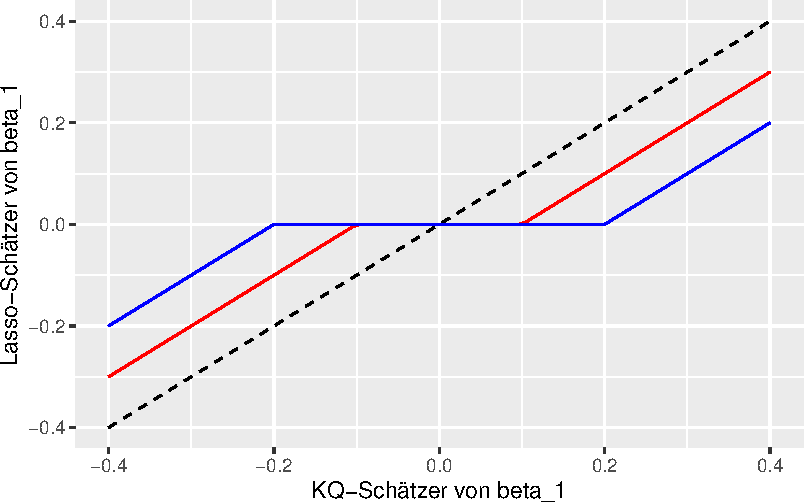
\includegraphics{RegReg_files/figure-pdf/fig-lassoST-1.pdf}

}

\caption{\label{fig-lassoST}Shrinkage und Selektion von
OLS-Koeffizienten mit Lasso}

\end{figure}

Abbildung~\ref{fig-lassoST} zeigt, dass der \(\ell_1\)-Strafterm des
Lasso-Schätzers zu einem linearen Verlauf der auf den KQ-Schätzer
(gezeichnet für \(\lambda = 0\), gestrichelte Linie) applizierten
Shrinkage führt: Der Lasso-Schätzer ist eine abschnittsweise-lineare
Funktion des KQ-Schätzers in \(\lambda\): Je größer der Parameter
\(\lambda\), desto größer ist das Intervall von KQ-Schätzwerten
\([-\lambda/2,\lambda/2]\), wo der Lasso-Schätzer zu Variablenselektion
führt, d.h. hier den Koeffizienten \(\beta_j\) als \(0\) schätzt (rote
bzw. blaue Linie).

Anhand von Abbildung~\ref{fig-lassoST} kann abgeleitet werden, dass der
Lasso-Schätzer nicht invariant gegenüber der Skalierung der Regressoren
ist: Die Stärke der Regularisierung durch \(\lambda\) ist hängt von der
Magnitude des KQ-Schätzers ab. Daher müssen die Regressoren vor
Berechnung der Schätzung standardsiert werden. Üblich ist hierbei eine
Normierung auf einen Mittelwert von \(0\) und eine Varianz von \(1\).

Die nachstehende interaktive Grafik illustriert das
Lasso-Optimierungsproblem \eqref{eq:lassolagrange} sowie den
resultierenden Schätzer der Koeffizienten \((\beta_1, \beta_2)\) in
einem multiplen Regressionsmodell mit korrelierten Regressoren \(X_1\)
und \(X_2\).

\begin{itemize}
\item
  Die blaue Ellipse ist die Menge aller Schätzwerte
  \(\left(\widehat\beta_{1},\, \widehat\beta_{2}\right)\) für den
  angegebenen Wert von \(\mathrm{RSS}\). Im Zentrum der Ellipse liegt
  der KQ-Schätzer, welcher \(\mathrm{RSS}\) minimiert.
\item
  Das graue Quadrat ist die Menge aller Koeffizienten-Paare
  \((\beta_1, \beta_2)\), welche die Restriktion
  \(\lvert\beta_1\rvert+\lvert\beta_2\rvert\leq t\) erfüllen. Beachte,
  dass die Größe dieser Region nur durch den Parameter \(t\) bestimmt
  wird.
\item
  Der blaue Punkt ist der Lasso-Schätzer
  \((\widehat{\boldsymbol{\beta}}^L_{1,t},\, \widehat{\boldsymbol{\beta}}^L_{2,t})\).
  Dieser ergibt sich als Schnittpunkt zwischen der blauen
  \(\mathrm{RSS}\)-Ellipse und der Restriktionsregion und variiert mit
  \(t\). Die gestrichelte rote Linie zeigt den Lasso-Lösungspfad.
\item
  Für kleine Werte, erhalten wir starke Shrinkage auf
  \(\widehat\beta_{1,t}\) bis zum Wertebereich \(t\leq50\), wo
  \(\widehat{\boldsymbol{\beta}}^L_{1,t}=0\). Hier erfolgt
  Variablenselektion: Die Regularisierung führt zu einem geschätzten
  Modell, das lediglich \(X_2\) als erklärende Variable enthält. In
  diesem Bereich von \(t\) bewirkt die Shrinkage, dass
  \(\widehat{\boldsymbol{\beta}}^L_{2,t}\to0\) für \(t\to0\).
\end{itemize}

\begin{center}\rule{0.5\linewidth}{0.5pt}\end{center}

\textbf{\emph{Diese Interaktive Komponente des Buchs ist nur in der
Online-Version verfügbar.}}

\begin{center}\rule{0.5\linewidth}{0.5pt}\end{center}

Beachte, dass der rote Lasso-Pfad (die Menge aller Lasso-Lösungen)
äquivalent als Funktion von \(\lambda\) im Optimierungsproblem
\eqref{eq:lassoloss} dargestellt werden kann. Implementierungen mit
statistischer Software berechnen die Lasso-Lösung häufig in Abhängigkeit
von \(\lambda\). Ein Algorithmus hierfür ist LARS.

\hypertarget{berechnung-der-lasso-luxf6sung-mit-dem-lars-algorithmus}{%
\subsection{Berechnung der Lasso-Lösung mit dem
LARS-Algorithmus}\label{berechnung-der-lasso-luxf6sung-mit-dem-lars-algorithmus}}

Für die Berechnung des Lasso-Lösungspfads kann der
\href{https://en.wikipedia.org/wiki/Least-angle_regression}{LARS-Algorithmus}
von Efron u.~a. (2004) im Lasso-Modus genutzt werden.\footnote{LARS
  steht für \emph{Least Angle Regression}.} Der Lasso-Lösungspfad
beinhaltet geschätzte Koeffizienten über ein Intervall für \(\lambda\),
welches sämtliche Modellkomplexitäten zwischen der (trivialen) Lösung
mit maximaler Shrinkage auf allen Koeffizienten (\(\lambda\) groß, alle
gesch. Koeffizienten sind \(0\)) und der unregularisierten Lösung
(\(\lambda = 0\), KQ-Schätzung) abbildet. Der LARS-Algorithmus erzeugt
den Lösungspfad sequentiell, sodass die Schätzung als Funktion von
\(\lambda\) veranschaulicht werden kann, ähnlich wie bei Ridge
Regression.

Wir zeigen nun anhand simulierter Daten, wie Lasso-Lösungen mit dem
R-Paket \texttt{lars} berechnet werden können. Hierfür erzeugen wir
Daten gemäß der Vorschrift \begin{align}
  \begin{split}
  Y_i =&\, \boldsymbol{X}_i' \boldsymbol{\beta}_v + u_i\\
  \\
  \boldsymbol{\beta}_v =&\, (-1.25, -.75, 0, 0, 0, 0, 0, .75, 1.25)'\\
  \\
  \boldsymbol{X}_i \sim&\, N(\boldsymbol{0}, \boldsymbol{I}_{9\times9}), \quad u_i \overset{u.i.v.}{\sim} N(0, 1), \quad i = 1,\dots,25.
  \end{split}\label{eq:larsdgp}
\end{align}

\begin{Shaded}
\begin{Highlighting}[]
\FunctionTok{library}\NormalTok{(lars)}
\FunctionTok{set.seed}\NormalTok{(}\DecValTok{1234}\NormalTok{)}

\CommentTok{\# Parameter definieren}
\NormalTok{N }\OtherTok{\textless{}{-}} \DecValTok{25}
\NormalTok{beta\_v }\OtherTok{\textless{}{-}} \FunctionTok{c}\NormalTok{(}\SpecialCharTok{{-}}\FloatTok{1.25}\NormalTok{, }\SpecialCharTok{{-}}\NormalTok{.}\DecValTok{75}\NormalTok{, }\DecValTok{0}\NormalTok{, }\DecValTok{0}\NormalTok{, }\DecValTok{0}\NormalTok{, }\DecValTok{0}\NormalTok{, }\DecValTok{0}\NormalTok{, .}\DecValTok{75}\NormalTok{, }\FloatTok{1.25}\NormalTok{)}

\CommentTok{\# Beobachtungen simulieren}
\NormalTok{X }\OtherTok{\textless{}{-}} \FunctionTok{matrix}\NormalTok{(}\FunctionTok{rnorm}\NormalTok{(N }\SpecialCharTok{*} \DecValTok{9}\NormalTok{), }\AttributeTok{ncol =} \DecValTok{9}\NormalTok{)}
\NormalTok{Y }\OtherTok{\textless{}{-}}\NormalTok{ X }\SpecialCharTok{\%*\%}\NormalTok{ beta\_v }\SpecialCharTok{+} \FunctionTok{rnorm}\NormalTok{(N)}
\end{Highlighting}
\end{Shaded}

Entsprechend des DGP passen wir ein Modell ohne Konstante an. Damit
\texttt{lars::lars()} den Lösungspfad des Lasso-Schätzers berechnet,
muss \texttt{type\ =\ "lasso"} gewählt werden.\footnote{\texttt{lars()}
  standardisiert die Regressoren standardmäßig (aufgrund des DGPs hier
  nicht nötig).}

\begin{Shaded}
\begin{Highlighting}[]
\CommentTok{\# Lösungen des Lasso{-}Schätzers mit LARS berechnen}
\NormalTok{(}
\NormalTok{  fit\_lars }\OtherTok{\textless{}{-}} \FunctionTok{lars}\NormalTok{(}
    \AttributeTok{x =}\NormalTok{ X, }
    \AttributeTok{y =}\NormalTok{ Y, }
    \AttributeTok{intercept =}\NormalTok{ F,}
    \AttributeTok{type =} \StringTok{"lasso"} \CommentTok{\# Wichtig: Lasso{-}Modus}
\NormalTok{  )}
\NormalTok{)}
\end{Highlighting}
\end{Shaded}

\begin{verbatim}

Call:
lars(x = X, y = Y, type = "lasso", intercept = F)
R-squared: 0.858 
Sequence of LASSO moves:
                      
Var  9 2 8 1 3 5 4 7 6
Step 1 2 3 4 5 6 7 8 9
\end{verbatim}

Die Zusammenfassung zeigt, dass der LARS-Algorithmus als erstes die
(relevante) Variable \(X_9\) aktiviert.\footnote{Aktivierung meint die
  Aufnahme einer Variable in der Modell gegeben eines hinreichend
  kleinen \(\lambda\).} Mit abnehmender Regularisierung (kleinere
\(\lambda\)) werden in den nächsten 3 Schritten die übrigen relevanten
Variablen \(X_2\), \(X_8\) und \(X_1\) aktiviert. Über die weiteren
Schritte nähert der Algorithmus die Lösung an die \emph{saturierte}
Schätzung (das Modell mit allen neun Regressoren) an und aktiviert
schrittweise die übrigen, irrelevanten Variablen.

Wir visualisieren die geschätzen Koeffizienten an jedem Schritt des
Lösungspfads als Funktion von \(\lambda\). In der Praxis wird der
Regularisierungsparameter häufig auf der natürlichen log-Skala
dargestellt.

\begin{Shaded}
\begin{Highlighting}[]
\CommentTok{\# Transformation in ein weites Format}
\NormalTok{fit\_lars}\SpecialCharTok{$}\NormalTok{beta }\SpecialCharTok{\%\textgreater{}\%} 
  \FunctionTok{as\_tibble}\NormalTok{() }\SpecialCharTok{\%\textgreater{}\%} 
  \FunctionTok{mutate}\NormalTok{(}
    \AttributeTok{lambda =} \FunctionTok{c}\NormalTok{(fit\_lars}\SpecialCharTok{$}\NormalTok{lambda, }\FloatTok{1e{-}2}\NormalTok{)}
\NormalTok{  ) }\SpecialCharTok{\%\textgreater{}\%} 
  \FunctionTok{pivot\_longer}\NormalTok{(}
    \AttributeTok{cols =} \DecValTok{1}\SpecialCharTok{:}\DecValTok{9}\NormalTok{, }
    \AttributeTok{names\_to =} \StringTok{"Variable"}\NormalTok{, }
    \AttributeTok{values\_to =} \StringTok{"gesch. Koeffizient"}
\NormalTok{  ) }\SpecialCharTok{\%\textgreater{}\%} 
  
\CommentTok{\# Visualisierung mit ggplot  }
  \FunctionTok{ggplot}\NormalTok{(}
    \AttributeTok{mapping =} \FunctionTok{aes}\NormalTok{(}
      \AttributeTok{x =} \FunctionTok{log}\NormalTok{(lambda), }
      \AttributeTok{y =} \StringTok{\textasciigrave{}}\AttributeTok{gesch. Koeffizient}\StringTok{\textasciigrave{}}\NormalTok{, }
      \AttributeTok{color =}\NormalTok{ Variable}
\NormalTok{    )}
\NormalTok{  ) }\SpecialCharTok{+} 
  \FunctionTok{geom\_line}\NormalTok{() }
\end{Highlighting}
\end{Shaded}

\begin{figure}[t]

{\centering 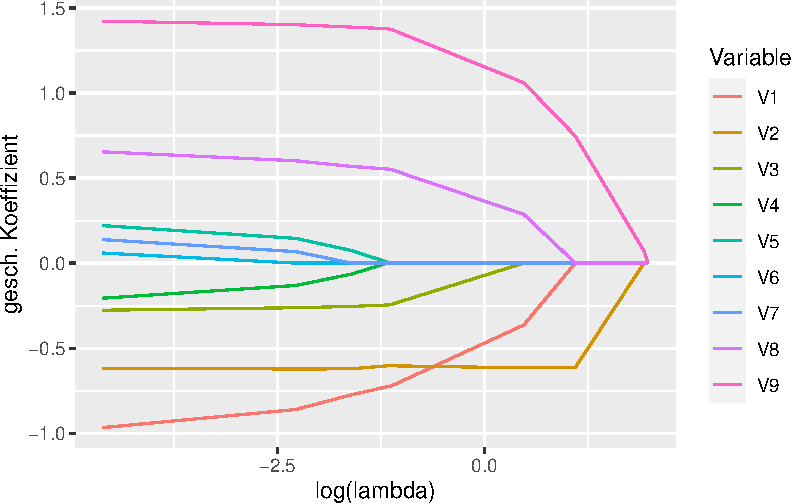
\includegraphics{RegReg_files/figure-pdf/fig-larssolpath-1.pdf}

}

\caption{\label{fig-larssolpath}LARS-Lösungspfad für Lasso-Schätzung}

\end{figure}

Abbildung~\ref{fig-larssolpath} zeigt, dass die Shrinkage der
geschätzten Koeffizienten nach der Aktivierung rasch abnimmt und sich
für kleine Werte von \(\lambda\) der KQ-Lösung annähert. Wir sehen auch,
dass es einen Bereich von \(\lambda\)-Werten gibt, für die das wahre
Modell mit den Variablen \(X_1\), \(X_2\), \(X_8\) und \(X_9\)
selektiert werden kann. Je nach Ziel der Analyse kann es sinnvoll sein,
ein \(\lambda\) in diesem Intervall zu schätzen.

\hypertarget{wahl-des-regularisierungsparameters-lambda-fuxfcr-den-lasso-schuxe4tzer}{%
\subsection{\texorpdfstring{Wahl des Regularisierungsparameters
\(\lambda\) für den
Lasso-Schätzer}{Wahl des Regularisierungsparameters \textbackslash lambda für den Lasso-Schätzer}}\label{wahl-des-regularisierungsparameters-lambda-fuxfcr-den-lasso-schuxe4tzer}}

Wie zuvor bei Ridge Regression muss in empirischen Anwendungen ein Wert
für den Tuning-Parameter \(\lambda\) gewählt werden. Hierbei besteht die
Herausforderung darin, einen geeigneten Wert zu finden, der zu
wünschenswerten Eigenschaften des resultierenden Modells führt. So ist
für gute Vorhersagen wichtig, dass das Modell nicht zu sehr an die Daten
angepasst ist (\emph{Overfitting}), um eine gute Generalisierung auf
neue Daten zu ermöglichen. Gleichzeitig muss das Modell flexibel genug
sein, um wesentliche Eigenschaften des datenerzeugenden Prozesses
hinreichend gut zu erfassen. In der Regel wird hierbei eine sparsame
Modellierung angestrebt, die nur eine Teilmenge der Prädiktoren nutzt.

In der Praxis werden verschiedene Verfahren verwendet, um den Wert für
den Tuning-Parameter \(\lambda\) zu bestimmen. Gängige Methoden sind
\emph{Cross Validation} (CV) und Informationskriterien. In Abhängigkeit
der Methode und der Daten ergeben sich ober- oder unterparameterisierte
Modelle. Aufgrund der Implementierung im R-Paket \texttt{lars}
betrachten wir CV.\footnote{Chetverikov, Liao, and Chernozhukov (2020)
  zeigen, dass CV zu konsistenter Modellselektion führen kann.} Wir
zeigen nachfolgend anhand der simulierten Daten aus dem letzten
Abschnitt, wie für die LARS-Schätzung ein optimales \(\lambda\) mit
leave-one-out CV (LOO-CV) bestimmt werden kann. Hierzu nutzen wir
\texttt{lars::cv.lars()} unter Verwendung derselben Argumente wie zuvor
im Aufruf von \texttt{lars()}.

\begin{Shaded}
\begin{Highlighting}[]
\CommentTok{\# LARS{-}Lösungen mit CV evaluieren}
\NormalTok{fit\_lars\_cv }\OtherTok{\textless{}{-}} \FunctionTok{cv.lars}\NormalTok{(}
  \AttributeTok{x =}\NormalTok{ X, }
  \AttributeTok{y =}\NormalTok{ Y, }
  \AttributeTok{intercept =}\NormalTok{ F,}
  \AttributeTok{normalize =}\NormalTok{ T,}
  \AttributeTok{type =} \StringTok{"lasso"}\NormalTok{, }
  \AttributeTok{plot.it =}\NormalTok{ F, }
  \AttributeTok{K =}\NormalTok{ N }\CommentTok{\# für LOO{-}CV}
\NormalTok{) }
\end{Highlighting}
\end{Shaded}

Das Objekt \texttt{fit\_lars\_cv} ist eine Liste mit den CV-Ergebnissen.
Wir können diese einfach mit \texttt{ggplot} visualisieren.
\texttt{index} ist hierbei das Verhältnis der \(\ell_1\)-Norm des
Lasso-Schätzers für einen spezifischen Wert von \(\lambda\) und der
\(\ell_1\)-Norm des KQ-Schätzers. Das optimale \(\lambda\) wird so
implizit geschätzt. \texttt{cv.error} ist der mit CV geschätzte MSE.

\begin{Shaded}
\begin{Highlighting}[]
\CommentTok{\# CV{-}MSE}
\NormalTok{fit\_lars\_cv }\SpecialCharTok{\%\textgreater{}\%} 
  \FunctionTok{as\_tibble}\NormalTok{() }\SpecialCharTok{\%\textgreater{}\%}

  \FunctionTok{ggplot}\NormalTok{(}
    \AttributeTok{mapping =} \FunctionTok{aes}\NormalTok{(}
      \AttributeTok{x =}\NormalTok{ index, }
      \AttributeTok{y =}\NormalTok{ cv.error}
\NormalTok{    )}
\NormalTok{  ) }\SpecialCharTok{+} 
  \FunctionTok{geom\_line}\NormalTok{() }\SpecialCharTok{+}
  \FunctionTok{xlab}\NormalTok{(}\StringTok{"|beta\_lambda| / |beta|"}\NormalTok{) }\SpecialCharTok{+}
  \FunctionTok{ylab}\NormalTok{(}\StringTok{"CV{-}MSE"}\NormalTok{)}
\end{Highlighting}
\end{Shaded}

\begin{figure}[t]

{\centering 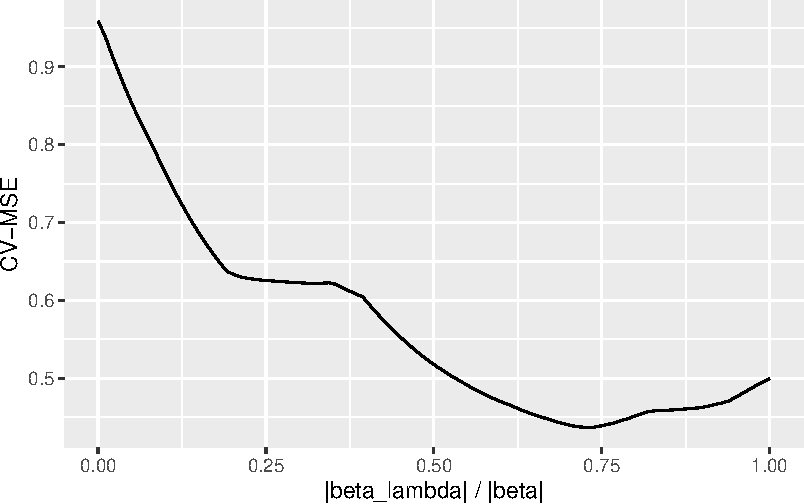
\includegraphics{RegReg_files/figure-pdf/fig-larscv-1.pdf}

}

\caption{\label{fig-larscv}CV-MSE und relative Position von \(\lambda\)
auf dem Lassopfad}

\end{figure}

In der Grafik erkennen wir ein Minimum des CV-MSEs bei etwa 0.73.

\begin{Shaded}
\begin{Highlighting}[]
\CommentTok{\# CV{-}MSE{-}minimierendes Lambda bestimmen}
\NormalTok{ID }\OtherTok{\textless{}{-}} \FunctionTok{which.min}\NormalTok{(fit\_lars\_cv}\SpecialCharTok{$}\NormalTok{cv.error) }\CommentTok{\# Index}

\NormalTok{(}
\NormalTok{  fraction\_opt }\OtherTok{\textless{}{-}}\NormalTok{ fit\_lars\_cv}\SpecialCharTok{$}\NormalTok{index[ID]}
\NormalTok{)}
\end{Highlighting}
\end{Shaded}

\begin{verbatim}
[1] 0.7272727
\end{verbatim}

Die geschätzten Koeffizienten für die optimale Regularisierung können
mit \texttt{coef()} ausgelesen werden.

\begin{Shaded}
\begin{Highlighting}[]
\CommentTok{\# LARS{-}Lasso{-}Fit für optimales lambda bestimmen}
\FunctionTok{coef}\NormalTok{(}
  \AttributeTok{object =}\NormalTok{ fit\_lars, }
  \AttributeTok{s =}\NormalTok{ fraction\_opt, }
  \AttributeTok{mode =} \StringTok{"fraction"}
\NormalTok{)}
\end{Highlighting}
\end{Shaded}

\begin{verbatim}
[1] -0.6513191 -0.6060906 -0.1946089  0.0000000  0.0000000  0.0000000  0.0000000
[8]  0.4977908  1.3122407
\end{verbatim}

Das Ergebnis veranschaulicht die Selektionseigenschaft von Lasso: Gemäß
DGP \eqref{eq:larsdgp} sind die Variablen \(X_3\) bis \(X_7\)
\emph{irrelevante} Prädiktoren für \(Y\); ihre wahren Koeffizienten sind
\(0\). In der kreuzvalidierten Lasso-Schätzung erreicht die
Regularisierung, dass die Koeffizienten der Variablen \(X_4\) bis
\(X_7\) tatsächlich mit 0 geschätzt werden. Wir schätzen für das mit CV
bestimmte \(\lambda\) also ein leicht überspezifiziertes Modell mit den
Regressoren \(X_1\), \(X_2\), \(X_3\), \(X_8\) und \(X_9\). Beachte,
dass die Lasso-Schätzung einen Kompromiss impliziert: Die Varianz der
Schätzung ist geringer als die des KQ-Schätzers im Modell mit allen
Variablen.\footnote{Wegen \(N=25\) verbleiben bei der KQ-Schätzung mit 9
  Regressoren nur 16 Freiheitsgrade.} Aufgrund der Regularisierung sind
die mit Lasso geschätzten Koeffizienten der relevanten Variablen jedoch
in Richtung \(0\) verzerrt.

Einen positiven Effekt dieses Kompromisses beobachten wir anhand des
mittleren Vorhersagefehlers für Daten, die \emph{nicht} zur Berechnung
des Schätzers verwendet wurden. Wir vergleichen den Vorhersagefehler
nachfolgend anhand eines solchen simulierten Test-Datensatzes mit 25
neuen Beobachtungen. Den Vorhersagefehler bestimmen wir als MSE zwischen
den vorhergesagten und den tatsächlichen Ausprägungen für \(Y\).

\begin{Shaded}
\begin{Highlighting}[]
\CommentTok{\# Test{-}Datensatz erstellen}
\FunctionTok{set.seed}\NormalTok{(}\DecValTok{4321}\NormalTok{)}
\NormalTok{new\_X }\OtherTok{\textless{}{-}} \FunctionTok{matrix}\NormalTok{(}\FunctionTok{rnorm}\NormalTok{(N }\SpecialCharTok{*} \DecValTok{9}\NormalTok{), }\AttributeTok{ncol =} \DecValTok{9}\NormalTok{)}
\NormalTok{new\_Y }\OtherTok{\textless{}{-}}\NormalTok{ new\_X }\SpecialCharTok{\%*\%}\NormalTok{ beta\_v }\SpecialCharTok{+} \FunctionTok{rnorm}\NormalTok{(N)}

\CommentTok{\# Lasso: Vorhersage von new\_Y für Test{-}Datensatz}
\NormalTok{Y\_predict\_lars }\OtherTok{\textless{}{-}} \FunctionTok{predict}\NormalTok{(}
  \AttributeTok{object =}\NormalTok{ fit\_lars, }
  \AttributeTok{s =}\NormalTok{ fraction\_opt, }
  \AttributeTok{type =} \StringTok{"fit"}\NormalTok{, }
  \AttributeTok{mode =} \StringTok{"fraction"}\NormalTok{, }
  \AttributeTok{newx =}\NormalTok{ new\_X}
\NormalTok{)}\SpecialCharTok{$}\NormalTok{fit}

\CommentTok{\# Lasso: MSE für Test{-}Datensatz berechnen}
\FunctionTok{mean}\NormalTok{((Y\_predict\_lars }\SpecialCharTok{{-}}\NormalTok{ new\_Y)}\SpecialCharTok{\^{}}\DecValTok{2}\NormalTok{)}
\end{Highlighting}
\end{Shaded}

\begin{verbatim}
[1] 1.419817
\end{verbatim}

Wir schätzen nun das große Modell mit allen 9 Variablen mit KQ und
berechnen ebenfalls den MSE der Prognosen für den Test-Datensatz.

\begin{Shaded}
\begin{Highlighting}[]
\CommentTok{\# KQ{-}Schätzung des großen Modells durchführen}
\NormalTok{KQ\_fit }\OtherTok{\textless{}{-}} \FunctionTok{lm}\NormalTok{(Y }\SpecialCharTok{\textasciitilde{}}\NormalTok{ X }\SpecialCharTok{{-}} \DecValTok{1}\NormalTok{)}

\CommentTok{\# Test{-}Datensatz für predict.lm() formatieren}
\NormalTok{new\_X }\OtherTok{\textless{}{-}} \FunctionTok{as.data.frame}\NormalTok{(new\_X)}
\FunctionTok{colnames}\NormalTok{(new\_X) }\OtherTok{\textless{}{-}} \FunctionTok{paste0}\NormalTok{(}\StringTok{"X"}\NormalTok{, }\DecValTok{1}\SpecialCharTok{:}\DecValTok{9}\NormalTok{)}

\CommentTok{\# KQ: Vorhersage von new\_Y für Test{-}Datensatz}
\NormalTok{Y\_predict\_KQ }\OtherTok{\textless{}{-}} \FunctionTok{predict}\NormalTok{(}
  \AttributeTok{object =}\NormalTok{ KQ\_fit, }
  \AttributeTok{newdata =}\NormalTok{ new\_X}
\NormalTok{)}

\CommentTok{\# KQ: MSE für Test{-}Datensatz berechnen}
\FunctionTok{mean}\NormalTok{((Y\_predict\_KQ }\SpecialCharTok{{-}}\NormalTok{ new\_Y)}\SpecialCharTok{\^{}}\DecValTok{2}\NormalTok{)}
\end{Highlighting}
\end{Shaded}

\begin{verbatim}
[1] 9.851932
\end{verbatim}

Offenbar führt die Lasso-Schätzung zu einem deutlich geringeren MSE der
Vorhersage von \texttt{Y} für den Test-Datensatz als die KQ-Schätzung
und damit zu einer höheren Vorhersagegüte. Das ``sparsame'' mit
Lasso-Regression geschätzte Modell ist dem ``großen'' mit KQ geschätztem
Modell in dieser Hinsicht also überlegen.

\begin{tcolorbox}[enhanced jigsaw, colbacktitle=quarto-callout-note-color!10!white, bottomtitle=1mm, breakable, leftrule=.75mm, opacityback=0, title=\textcolor{quarto-callout-note-color}{\faInfo}\hspace{0.5em}{Key Facts zu Lasso-Regression}, left=2mm, arc=.35mm, titlerule=0mm, bottomrule=.15mm, opacitybacktitle=0.6, coltitle=black, toptitle=1mm, colback=white, colframe=quarto-callout-note-color-frame, toprule=.15mm, rightrule=.15mm]

\begin{itemize}
\item
  Lasso-Regression bestraft die Verlustfunktion des KQ-Schätzers mit der
  \(\ell_1\)-Norm der Koeffizienten.
\item
  Neben Koeffizientenschätzung mit Shrinkage in Richtung \(0\) kann der
  Lasso-Schätzer Variablenselektion durchführen:
  Regressionskoeffizienten können exakt mit \(0\) geschätzt und so ein
  ``sparsames'', leichter zu interpretierendes Modell gewählt werden.
\item
  Wie bei Ridge Regression impliziert die Wahl von \(\lambda\) einen
  Bias-Variance-Tradeoff, der für Vorhersagen nützlich ist: Für größere
  \(\lambda\) wird mehr Verzerrung induziert und möglicherweise
  relevante Variablen mit kleinen Koeffizienten aus dem Modell entfernt.
  Ein solches sparsames Modell kann eine höhere Prognosegüte haben als
  ein komplexes, unregularisiertes Modell.
\item
  Der Lasso-Schätzer \(\widehat{\boldsymbol{\beta}}_\lambda^L\) ist
  \emph{nicht} erwartungstreu.
\item
  Lasso Regression kann bspw. mit dem LARS-Algorithmus (Paket
  \texttt{lars}) oder mit \texttt{glmnet} berechnet werden.
\end{itemize}

\end{tcolorbox}

\hypertarget{vergleich-von-lasso--und-ridge-regression-mit-simulation}{%
\section{Vergleich von Lasso- und Ridge-Regression mit
Simulation}\label{vergleich-von-lasso--und-ridge-regression-mit-simulation}}

In diesem Kapitel illustrieren wir Vor- und Nachteile von Lasso- und
Ridge-Regression in Prognose-Anwendungen anhand von
Monte-Carlo-Simulationen. Wir betrachten hierbei datenerzeugende
Prozesse, die sich hinsichtlich der Anzahl relevanter Variablen sowie
der Korrelation dieser Variablen unterscheiden.

Die grundlegende Vorschrift für die Simulationen ist \begin{align*}
  Y_i = \sum_{j=1}^{k=40} \beta_j X_{i,j} + u_i, \quad u_i \overset{u.i.v.}{\sim} N(0,1), \quad i=1,\dots,100,
\end{align*} wobei die Regressoren \(X_j\) eine Varianz von \(1\) haben
und aus einer multivariaten Normalverteilung mit Korrelation
\[\rho\in(0,0.5,0.8)\] gezogen werden.

Für die Koeffizienten \(\boldsymbol{\beta}\) unterscheiden wir zwei
Szenarien. In Szenario A ist \[\boldsymbol{\beta} = (1,\dots,1)',\] d.h.
alle Variablen sind relevant und haben denselben Einfluss auf \(Y\). In
Szenario B erzeugen wir \(\boldsymbol{\beta}\) einmalig vorab so, dass
\[\beta_j = \begin{cases}1,\quad \text{mit Wsk.  }p\\ 0,\quad \text{mit Wsk.  }1-p, \end{cases}\]
d.h. nur eine Teilmenge der Variablen beeinflusst \(Y\) jeweils mit
demselben Effekt \(\beta_j = 1\). Die übrigen Variablen sind irrelevant.

Wir schätzen und validieren die Modelle mit \texttt{glmnet()}.

\hypertarget{sec-pdz}{%
\subsection{Prognosegüte in diversen Szenarien}\label{sec-pdz}}

\begin{Shaded}
\begin{Highlighting}[]
\CommentTok{\# Simulationsparameter definieren}
\NormalTok{rho }\OtherTok{\textless{}{-}} \FunctionTok{c}\NormalTok{(}\DecValTok{0}\NormalTok{, }\FloatTok{0.5}\NormalTok{, }\FloatTok{0.8}\NormalTok{)   }\CommentTok{\# Korrelation}
\NormalTok{k }\OtherTok{\textless{}{-}} \DecValTok{40}                 \CommentTok{\# Anz. Regressoren}
\NormalTok{N }\OtherTok{\textless{}{-}} \DecValTok{100}                \CommentTok{\# Anz. Beobachtungen}
\NormalTok{n\_sim }\OtherTok{\textless{}{-}} \DecValTok{100}            \CommentTok{\# Anz. Simulationen}
\end{Highlighting}
\end{Shaded}

Damit der Code für die Simulation möglichst wenig repetitiv ist,
definieren wir eine Funktion \texttt{cv.glmnet\_MSE()}, die unter Angabe
der Daten \texttt{X} und \texttt{Y}, des Trainingssets \texttt{train}
sowie des Parameters \texttt{alpha} den gewünschten regularisierten
Schätzer under Verwendung von Cross Validation anpasst und den
Testset-MSE zurückgibt.

\begin{Shaded}
\begin{Highlighting}[]
\CommentTok{\# allg. Funktion für Testset{-}MSE nach CV}
\NormalTok{cv.glmnet\_MSE }\OtherTok{\textless{}{-}} \ControlFlowTok{function}\NormalTok{(X, Y, train, alpha) \{}
  
  \CommentTok{\# Modell mit glmnet schätzen; lambda per CV bestimmen}
\NormalTok{  fit\_cv }\OtherTok{\textless{}{-}} \FunctionTok{cv.glmnet}\NormalTok{(}
    \AttributeTok{x =}\NormalTok{ X[train,],}
    \AttributeTok{y =}\NormalTok{Y[train],}
    \AttributeTok{alpha =}\NormalTok{ alpha}
\NormalTok{  )}
  
  \CommentTok{\# Vorhersagen treffen}
\NormalTok{  Y\_pred }\OtherTok{\textless{}{-}} \FunctionTok{predict}\NormalTok{(}
    \AttributeTok{object =}\NormalTok{ fit\_cv, }
    \AttributeTok{s =}\NormalTok{ fit\_cv}\SpecialCharTok{$}\NormalTok{lambda.min, }
    \AttributeTok{newx =}\NormalTok{ X[}\SpecialCharTok{{-}}\NormalTok{train,])}
  
  \FunctionTok{return}\NormalTok{(}
    \CommentTok{\# Testset{-}MSE berechnen}
    \FunctionTok{mean}\NormalTok{(}
\NormalTok{      (Y[}\SpecialCharTok{{-}}\NormalTok{train] }\SpecialCharTok{{-}}\NormalTok{ Y\_pred)}\SpecialCharTok{\^{}}\DecValTok{2}
\NormalTok{      )}
\NormalTok{  )}
\NormalTok{\}}
\end{Highlighting}
\end{Shaded}

Wir initialisieren zunächst Matrizen, in welche die MSEs aus den 100
Simulationsdurchläufen reihenweise geschrieben werden.
\texttt{lasso\_mse} und \texttt{ridge\_mse} haben je eine Spalte für
jede Korrelation in \texttt{rho}

\begin{Shaded}
\begin{Highlighting}[]
\CommentTok{\# Matrizen für simulierte MSEs initialisieren...}
\NormalTok{lasso\_mse }\OtherTok{\textless{}{-}} \FunctionTok{matrix}\NormalTok{(}
  \AttributeTok{data =} \ConstantTok{NA}\NormalTok{, }
  \AttributeTok{nrow =}\NormalTok{ n\_sim, }
  \AttributeTok{ncol =} \FunctionTok{length}\NormalTok{(rho)}
\NormalTok{) }
\NormalTok{ridge\_mse }\OtherTok{\textless{}{-}}\NormalTok{ lasso\_mse}

\CommentTok{\# ... und benennen}
\FunctionTok{colnames}\NormalTok{(lasso\_mse) }\OtherTok{\textless{}{-}} \FunctionTok{paste0}\NormalTok{(}\StringTok{"Kor="}\NormalTok{, rho)}
\FunctionTok{colnames}\NormalTok{(ridge\_mse) }\OtherTok{\textless{}{-}} \FunctionTok{colnames}\NormalTok{(lasso\_mse)}
\end{Highlighting}
\end{Shaded}

Für die Simulation iterieren wir mit \texttt{purrr::walk} über den
Vektor \texttt{rho} sowie über die Laufvariable \texttt{1:n\_sim}. Beide
Schleifen nutzen den Syntax für anonyme Funktionen:

\begin{Shaded}
\begin{Highlighting}[]
\CommentTok{\# Die anonyme Funktion}
\ControlFlowTok{function}\NormalTok{(x) }\FunctionTok{return}\NormalTok{(x)}
\CommentTok{\# ist äquivalent definiert als}
\NormalTok{\textbackslash{}(x) }\FunctionTok{return}\NormalTok{(x)}
\end{Highlighting}
\end{Shaded}

In jeden Simulationsdurchlauf erzeugen wir den Datensatz entsprechend
der obigen Vorschrift, teilen die Daten auf und berechnen MSEs für
Lasso- und Ridge-Regression mit \texttt{cv.glmnet\_MSE()}.

\textbf{Szenario A}

\begin{Shaded}
\begin{Highlighting}[]
\CommentTok{\# Koeffizienten{-}Vektor definieren}
\NormalTok{beta }\OtherTok{\textless{}{-}} \FunctionTok{rep}\NormalTok{(}\DecValTok{1}\NormalTok{, k) }
\end{Highlighting}
\end{Shaded}

\begin{Shaded}
\begin{Highlighting}[]
\FunctionTok{library}\NormalTok{(mvtnorm)}
\FunctionTok{library}\NormalTok{(tidyverse)}

\FunctionTok{set.seed}\NormalTok{(}\DecValTok{1234}\NormalTok{)}

\CommentTok{\# Simulation durchführen}
\FunctionTok{walk}\NormalTok{(}\DecValTok{1}\SpecialCharTok{:}\FunctionTok{length}\NormalTok{(rho), \textbackslash{}(j) \{}
  
  \CommentTok{\# Korrelationsmatrix definieren}
\NormalTok{  Sigma }\OtherTok{\textless{}{-}} \FunctionTok{matrix}\NormalTok{(}
    \AttributeTok{data =}\NormalTok{ rho[j], }
    \AttributeTok{nrow =}\NormalTok{ k, }
    \AttributeTok{ncol =}\NormalTok{ k}
\NormalTok{  )}
  \FunctionTok{diag}\NormalTok{(Sigma) }\OtherTok{\textless{}{-}} \DecValTok{1}
  
  \FunctionTok{walk}\NormalTok{(}\DecValTok{1}\SpecialCharTok{:}\NormalTok{n\_sim, \textbackslash{}(i) \{}
    
  \CommentTok{\# Daten simulieren}
\NormalTok{  X }\OtherTok{\textless{}{-}} \FunctionTok{rmvnorm}\NormalTok{(}
    \AttributeTok{n =}\NormalTok{ N, }
    \AttributeTok{mean =} \FunctionTok{rep}\NormalTok{(}\DecValTok{0}\NormalTok{, k), }
    \AttributeTok{sigma =}\NormalTok{ Sigma}
\NormalTok{  )}
\NormalTok{  Y }\OtherTok{\textless{}{-}}\NormalTok{ X }\SpecialCharTok{\%*\%}\NormalTok{ beta }\SpecialCharTok{+} \FunctionTok{rnorm}\NormalTok{(N)}
    
  \CommentTok{\# Trainingsdaten definieren}
\NormalTok{  ID\_train }\OtherTok{\textless{}{-}} \FunctionTok{sample}\NormalTok{(}
    \AttributeTok{x =} \FunctionTok{c}\NormalTok{(}\DecValTok{1}\SpecialCharTok{:}\NormalTok{N), }
    \AttributeTok{size =}\NormalTok{ N}\SpecialCharTok{/}\DecValTok{2}
\NormalTok{  )}
    
  \CommentTok{\# Modelle mit CV schätzen und MSEs berechnen}
  \CommentTok{\# Ridge{-}Regression}
\NormalTok{  ridge\_mse[i, j] }\OtherTok{\textless{}\textless{}{-}} \FunctionTok{cv.glmnet\_MSE}\NormalTok{(}
    \AttributeTok{X =}\NormalTok{ X, }
    \AttributeTok{Y =}\NormalTok{ Y, }
    \AttributeTok{train =}\NormalTok{ ID\_train, }
    \AttributeTok{alpha =} \DecValTok{0}
\NormalTok{  )}
  
  \CommentTok{\# Lasso{-}Regression}
\NormalTok{  lasso\_mse[i, j] }\OtherTok{\textless{}\textless{}{-}} \FunctionTok{cv.glmnet\_MSE}\NormalTok{(}
    \AttributeTok{X =}\NormalTok{ X, }
    \AttributeTok{Y =}\NormalTok{ Y, }
    \AttributeTok{train =}\NormalTok{ ID\_train, }
    \AttributeTok{alpha =} \DecValTok{1}
\NormalTok{  )}
  
\NormalTok{  \})}
  
\NormalTok{\})}
\end{Highlighting}
\end{Shaded}

Beachte, dass hier der Super-Assignment-Operator
\texttt{\textless{}\textless{}-} genutzt wird, damit \texttt{walk} die
Matrizen \texttt{ridge\_mse} und \texttt{lasso\_mse} in der globalen
Umgebung überschreibt.\footnote{Dies folgt aus der Definition von
  \texttt{walk}. \texttt{\textless{}-} bewirkt hier lediglich Assignment
  in der Funktionsumgebung.}

Wir berechnen jeweils den mittleren MSEs, sammeln die Ergebnisse in
einer \texttt{tibble()} und nutzen \texttt{gt()} für die tabellarische
Darstellung.

\begin{Shaded}
\begin{Highlighting}[]
\FunctionTok{library}\NormalTok{(gt)}

\CommentTok{\# Ergebnisse tabellarisch darstellen}
\FunctionTok{tibble}\NormalTok{(}
  \AttributeTok{Methode =} \FunctionTok{c}\NormalTok{(}
    \StringTok{"Lasso{-}Regression"}\NormalTok{, }
    \StringTok{"Ridge{-}Regression"}
\NormalTok{  ),}
\NormalTok{) }\SpecialCharTok{\%\textgreater{}\%}
  \FunctionTok{bind\_cols}\NormalTok{(}
    \FunctionTok{bind\_rows}\NormalTok{(}
      \FunctionTok{colMeans}\NormalTok{(lasso\_mse),}
      \FunctionTok{colMeans}\NormalTok{(ridge\_mse)  }
\NormalTok{    )    }
\NormalTok{  ) }\SpecialCharTok{\%\textgreater{}\%}
  \FunctionTok{gt}\NormalTok{() }\SpecialCharTok{\%\textgreater{}\%}
\NormalTok{  tabopts}
\end{Highlighting}
\end{Shaded}

\hypertarget{tbl-lrsimA}{}
\begin{longtable}{lrrr}
\caption{\label{tbl-lrsimA}Durchschnittliche Testset-MSEs für Setting A }\tabularnewline

\toprule
Methode & Kor=0 & Kor=0.5 & Kor=0.8 \\ 
\midrule\addlinespace[2.5pt]
Lasso-Regression & $7.17$ & $10.398$ & $7.581$ \\ 
Ridge-Regression & $4.841$ & $1.615$ & $1.517$ \\ 
\bottomrule
\end{longtable}

Tabelle~\ref{tbl-lrsimA} zeigt, dass Ridge-Regression gegenüber
Lasso-Regression für jede der drei betrachteten Korrelationen überlegen
ist. Insbesondere bei stärker korrelierten Regressoren ist Ridge
vorteilhaft.

Für Szenario B überschreiben wir \texttt{beta} nach Multiplikation mit
einem zufälligen binären Vektor, sodass einige der Koeffizienten \(0\)
und die zugehörigen Variablen irrelevant für \(Y\) sind.

\textbf{Szenario B}

\begin{Shaded}
\begin{Highlighting}[]
\CommentTok{\# Wsk. für Relevanz einer Variable}
\NormalTok{p }\OtherTok{\textless{}{-}}\NormalTok{ .}\DecValTok{3}

\CommentTok{\# Koeffizienten{-}Vektor definieren}
\FunctionTok{set.seed}\NormalTok{(}\DecValTok{123}\NormalTok{)}
\NormalTok{beta }\OtherTok{\textless{}{-}}\NormalTok{ beta }\SpecialCharTok{*} \FunctionTok{sample}\NormalTok{(}
  \AttributeTok{x =} \DecValTok{0}\SpecialCharTok{:}\DecValTok{1}\NormalTok{, }
  \AttributeTok{size =}\NormalTok{ k, }
  \AttributeTok{replace =}\NormalTok{ T, }
  \AttributeTok{prob =} \FunctionTok{c}\NormalTok{(}\DecValTok{1}\SpecialCharTok{{-}}\NormalTok{p, p)}
\NormalTok{)}

\CommentTok{\# Koeffizienten prüfen}
\FunctionTok{head}\NormalTok{(beta, }\AttributeTok{n =} \DecValTok{10}\NormalTok{)}
\end{Highlighting}
\end{Shaded}

\begin{verbatim}
 [1] 0 1 0 1 1 0 0 1 0 0
\end{verbatim}

Eine wiederholung der Simulation für die modifizierten Koeffizienten
\texttt{beta} und liefert folgende tabellarische Auswertung.

\hypertarget{tbl-lrsimB}{}
\begin{longtable}{lrrr}
\caption{\label{tbl-lrsimB}Durchschnittliche Testset-MSEs für Szenario B }\tabularnewline

\toprule
Methode & Kor=0 & Kor=0.5 & Kor=0.8 \\ 
\midrule\addlinespace[2.5pt]
Lasso & $2.51$ & $2.143$ & $1.923$ \\ 
Ridge & $3.331$ & $2.562$ & $2.014$ \\ 
\bottomrule
\end{longtable}

Die Ergebnisse in Tabelle~\ref{tbl-lrsimB} zeigen, dass Ridge-Regression
in Szenario B bis auf den Fall unkorrelierter Regressoren etwas
schlechter abschneidet als in Szenario A. Die hohe Anzahl irrelevanter
Variablen verbessert die Leistung von Lasso deutlich: Hier ist es
plausibel, dass Lasso aufgrund der Thresholding-Eigenschaft die
Koeffizienten einiger irrelevanten Variablen häufig exakt \(0\) setzt
und damit ein sparsameres Modell schätzt als Ridge. Entsprechend erzielt
Lasso in diesem Szenario insbesondere für \(\rho = 0\) genauere
Vorhersagen als Ridge Regression.

\hypertarget{visualisierung-des-bias-variance-tradeoffs-bei-prognosen}{%
\subsection{Visualisierung des Bias-Variance-Tradeoffs bei
Prognosen}\label{visualisierung-des-bias-variance-tradeoffs-bei-prognosen}}

Für ein besseres Verständnis, wie sich der Regularisierungsparameter
\(\lambda\) auf den Bias-Variance-Tradeoff bei Prognosen mit Ridge- und
Lasso-Regression auswirkt, vergleichen wir für beide Methoden
nachfolgend die Abhängigkeit des MSEs der Prognose \(\widehat{Y}_0\) für
den Wert \(Y_0\) der abhängigen Variable eines Datenpunkts anhand seiner
Regressoren \(\boldsymbol{X}_0'\), wobei \begin{align}
  \text{MSE}(\widehat{Y}_0) = \text{Bias}(\widehat{Y}_0)^2 + \text{Var}(\widehat{Y}_0) + \text{Var}(Y_0) \label{eq:pbvdecomp}
\end{align} Beachte, dass \(\text{Var}(Y_0)\) die durch den
datenerzeugenden Prozess (und damit unvermeidbare) Varianz von \(Y_0\)
ist, wohingegen \(\text{Bias}(\widehat{Y}_0)^2\) und
\(\text{Var}(\widehat{Y}_0)\) von dem verwendeten Schätzer für
\(\widehat{Y}_0\) abhängt.

Für die Simulation betrachten wir erneut Szenario A aus
Kapitel~\ref{sec-pdz} mit \(50\) Beobachtungen für ein Modell mit \(40\)
unkorrelierten Regressoren. Wir legen zunächst die Simulationsparameter
fest und erzeugen den vorherzusagenden Datenpunkt (\texttt{X\_0},
\texttt{Y\_0}).

\begin{Shaded}
\begin{Highlighting}[]
\CommentTok{\# Parameter festlegen}
\FunctionTok{set.seed}\NormalTok{(}\DecValTok{1234}\NormalTok{)}
\NormalTok{n }\OtherTok{\textless{}{-}} \DecValTok{200} \CommentTok{\# Anz. Iterationen}
\NormalTok{N }\OtherTok{\textless{}{-}} \DecValTok{50}  \CommentTok{\# Anz. Beobachtungen}
\NormalTok{k }\OtherTok{\textless{}{-}} \DecValTok{40}  \CommentTok{\# Anz. Variablen}

\CommentTok{\# Korrelationsmatrix definieren}
\NormalTok{Sigma }\OtherTok{\textless{}{-}} \FunctionTok{diag}\NormalTok{(k) }\CommentTok{\# Diagonalmatrix}
\NormalTok{beta }\OtherTok{\textless{}{-}} \FunctionTok{rep}\NormalTok{(}\AttributeTok{x =} \DecValTok{1}\NormalTok{, k)}

\CommentTok{\# Prognose{-}Ziel vorab zufällig generieren:}

\CommentTok{\# Regressoren}
\NormalTok{X\_0 }\OtherTok{\textless{}{-}} \FunctionTok{rmvnorm}\NormalTok{(}
  \AttributeTok{n =} \DecValTok{1}\NormalTok{, }
  \AttributeTok{mean =} \FunctionTok{rep}\NormalTok{(}\AttributeTok{x =} \DecValTok{0}\NormalTok{, k)}
\NormalTok{)}

\CommentTok{\# Abh. Variable}
\NormalTok{Y\_0 }\OtherTok{\textless{}{-}}\NormalTok{ X\_0 }\SpecialCharTok{\%*\%}\NormalTok{ beta }\SpecialCharTok{+} \FunctionTok{rnorm}\NormalTok{(}\AttributeTok{n =} \DecValTok{1}\NormalTok{) }\SpecialCharTok{\%\textgreater{}\%} 
  \FunctionTok{as.vector}\NormalTok{()}
\end{Highlighting}
\end{Shaded}

Anhand der Simulationsergebnisse wollen wir die von der verwendeten
Schätzfunktion abhängigen Komponenten von \eqref{eq:pbvdecomp}
untersuchen. Wir initialisieren hierzu die Listen \texttt{ridge\_fits}
und \texttt{lasso\_fits}, in die unsere Simulationsergebnisse
geschrieben werden.

\begin{Shaded}
\begin{Highlighting}[]
\CommentTok{\# Listen für Simulationsergebnisse initialisieren}
\NormalTok{ridge\_fits }\OtherTok{\textless{}{-}} \FunctionTok{list}\NormalTok{()}
\NormalTok{lasso\_fits }\OtherTok{\textless{}{-}} \FunctionTok{list}\NormalTok{()}
\end{Highlighting}
\end{Shaded}

Weiterhin definieren wir separate \(\lambda\)-Sequenzen für Lasso- und
Ridge-Schätzer.\footnote{Die Sequenzen haben wir in Abhängigkeit des DGP
  so gewählt, dass die Abhängigkeit der Prognosegüte von \(\lambda\) gut
  visualisiert werden kann.}

\begin{Shaded}
\begin{Highlighting}[]
\CommentTok{\# Lambda{-}Sequenzen festlegen}
\NormalTok{lambdas\_r }\OtherTok{\textless{}{-}} \FunctionTok{seq}\NormalTok{(.}\DecValTok{25}\NormalTok{, }\FloatTok{2.5}\NormalTok{, }\AttributeTok{length.out =} \DecValTok{100}\NormalTok{)}
\NormalTok{lambdas\_l }\OtherTok{\textless{}{-}} \FunctionTok{seq}\NormalTok{(.}\DecValTok{05}\NormalTok{, }\FloatTok{0.5}\NormalTok{, }\AttributeTok{length.out =} \DecValTok{100}\NormalTok{)}
\end{Highlighting}
\end{Shaded}

Für die Simulation iterieren wir mit \texttt{walk()} über simulierte
Datensätze und schreiben jeweils den vollständigen Output von
\texttt{glmnet()} in die zuvor definierten Listen \texttt{ridge\_fits}
und \texttt{lasso\_fits}.

\begin{Shaded}
\begin{Highlighting}[]
\CommentTok{\# Simulation}
\FunctionTok{walk}\NormalTok{(}\DecValTok{1}\SpecialCharTok{:}\NormalTok{n, \textbackslash{}(i) \{}
  
  \CommentTok{\# Daten simulieren}
\NormalTok{  X }\OtherTok{\textless{}{-}} \FunctionTok{rmvnorm}\NormalTok{(}
    \AttributeTok{n =}\NormalTok{ N, }
    \AttributeTok{mean =} \FunctionTok{rep}\NormalTok{(}\DecValTok{0}\NormalTok{, k), }
    \AttributeTok{sigma =}\NormalTok{ Sigma}
\NormalTok{  )}
\NormalTok{  Y }\OtherTok{\textless{}{-}}\NormalTok{ X }\SpecialCharTok{\%*\%}\NormalTok{ beta }\SpecialCharTok{+} \FunctionTok{rnorm}\NormalTok{(}\AttributeTok{n =}\NormalTok{ N, }\AttributeTok{sd =} \DecValTok{5}\NormalTok{)}
  
  \CommentTok{\# Modelle mit glmnet schätzen}
  \CommentTok{\# Ridge{-}Regression}
\NormalTok{  ridge\_fits[[i]] }\OtherTok{\textless{}\textless{}{-}} \FunctionTok{glmnet}\NormalTok{(}
    \AttributeTok{x =}\NormalTok{ X, }
    \AttributeTok{y =}\NormalTok{ Y, }
    \AttributeTok{alpha =} \DecValTok{0}\NormalTok{, }
    \AttributeTok{intercept =}\NormalTok{ F}
\NormalTok{  )}
  \CommentTok{\# Lasso{-}Regression}
\NormalTok{  lasso\_fits[[i]] }\OtherTok{\textless{}\textless{}{-}} \FunctionTok{glmnet}\NormalTok{(}
    \AttributeTok{x =}\NormalTok{ X, }
    \AttributeTok{y =}\NormalTok{ Y, }
    \AttributeTok{alpha =} \DecValTok{1}\NormalTok{, }
    \AttributeTok{intercept =}\NormalTok{ F}
\NormalTok{  )}
  
\NormalTok{\})}
\end{Highlighting}
\end{Shaded}

Wir nutzen Funktionen aus \texttt{purrr} und \texttt{dplyr}, um über die
in den Simulationsdurchläufen angepassten Modelle zu iterieren. Mit
\texttt{predict()} erhalten wir Punktvorhersagen für \texttt{Y\_0} für
jedes \(\lambda\) der zuvor definierten \(\lambda\)-Sequenzen. Beachte,
dass \texttt{map()} jeweils eine Liste mit 200 Punktvorhersagen für
jedes der 100 zurückgibt. Mit \texttt{list\_rbind()} können wir die
Ergebnisse komfortabel jeweils in einer \texttt{tibble} sammeln.

\begin{Shaded}
\begin{Highlighting}[]
\CommentTok{\# Prognosen für Ridge{-}Regression}
\NormalTok{pred\_r }\OtherTok{\textless{}{-}} \FunctionTok{map}\NormalTok{(}
  \AttributeTok{.x =}\NormalTok{ ridge\_fits, }
  \AttributeTok{.f =} \SpecialCharTok{\textasciitilde{}} \FunctionTok{as\_tibble}\NormalTok{(}
    \FunctionTok{predict}\NormalTok{(}
      \AttributeTok{object =}\NormalTok{ ., }
      \AttributeTok{s =}\NormalTok{ lambdas\_r, }
      \AttributeTok{newx =}\NormalTok{ X\_0}
\NormalTok{    )}
\NormalTok{  ) }
\NormalTok{) }\SpecialCharTok{\%\textgreater{}\%}
  \FunctionTok{list\_rbind}\NormalTok{() }

\CommentTok{\# Prognosen für Lasso{-}Regression}
\NormalTok{pred\_l }\OtherTok{\textless{}{-}} \FunctionTok{map}\NormalTok{(}
  \AttributeTok{.x =}\NormalTok{ lasso\_fits, }
  \AttributeTok{.f =} \SpecialCharTok{\textasciitilde{}} \FunctionTok{as\_tibble}\NormalTok{(}
    \FunctionTok{predict}\NormalTok{(}
      \AttributeTok{object =}\NormalTok{ ., }
      \AttributeTok{s =}\NormalTok{ lambdas\_l, }
      \AttributeTok{newx =}\NormalTok{ X\_0)}
\NormalTok{    ) }
\NormalTok{) }\SpecialCharTok{\%\textgreater{}\%}
  \FunctionTok{list\_rbind}\NormalTok{() }
\end{Highlighting}
\end{Shaded}

Für die statistische Auswertung berechnen wir jeweils
\(\text{MSE}(\widehat{Y}_0)\), \(\text{Bias}(\widehat{Y}_0)^2\) und
\(\text{Var}(\widehat{Y}_0)\) und führen die Ergebnisse mit
\texttt{pivot\_longer()} in ein langes Format \texttt{sim\_data\_r}
über. Wir berechnen weiterhin mit \texttt{MSE\_min\_r} das \(\lambda\),
für das wir über die Simulationsdurchläufe durchschnittlich den
geringsten \(\text{MSE}\) beobachten.

\textbf{Ridge-Regression}

\begin{Shaded}
\begin{Highlighting}[]
\CommentTok{\# Ergebnisse für Ridge{-}Regression zusammenfassen}
\NormalTok{sim\_data\_r }\OtherTok{\textless{}{-}} \FunctionTok{tibble}\NormalTok{(}
  
  \AttributeTok{lambda =}\NormalTok{ lambdas\_r,}
  
  \StringTok{"MSE"} \OtherTok{=} \FunctionTok{map\_dbl}\NormalTok{(}
    \AttributeTok{.x =}\NormalTok{ pred\_r,  }
    \AttributeTok{.f =} \SpecialCharTok{\textasciitilde{}} \FunctionTok{mean}\NormalTok{((.x }\SpecialCharTok{{-}}\NormalTok{ Y\_0)}\SpecialCharTok{\^{}}\DecValTok{2}\NormalTok{)}
\NormalTok{  ),}
  
  \StringTok{"Bias\^{}2"} \OtherTok{=} \FunctionTok{map\_dbl}\NormalTok{(}
    \AttributeTok{.x =}\NormalTok{ pred\_r, }
    \AttributeTok{.f =} \SpecialCharTok{\textasciitilde{}}\NormalTok{ (}\FunctionTok{mean}\NormalTok{(.x) }\SpecialCharTok{{-}}\NormalTok{ Y\_0)}\SpecialCharTok{\^{}}\DecValTok{2}
\NormalTok{  ),}
  
  \StringTok{"Varianz"} \OtherTok{=} \FunctionTok{map\_dbl}\NormalTok{(}
    \AttributeTok{.x =}\NormalTok{ pred\_r, }
    \AttributeTok{.f =} \SpecialCharTok{\textasciitilde{}} \FunctionTok{var}\NormalTok{(.x)}
\NormalTok{  )}
\NormalTok{) }\SpecialCharTok{\%\textgreater{}\%}
  \FunctionTok{pivot\_longer}\NormalTok{(}
    \AttributeTok{cols =} \SpecialCharTok{{-}}\NormalTok{lambda, }
    \AttributeTok{values\_to =} \StringTok{"Wert"}\NormalTok{,}
    \AttributeTok{names\_to =} \StringTok{"Statistik"}
\NormalTok{  )}

\CommentTok{\# Lambda bei MSE{-}Minimum bestimmen}
\NormalTok{MSE\_min\_r }\OtherTok{\textless{}{-}}\NormalTok{ sim\_data\_r }\SpecialCharTok{\%\textgreater{}\%} 
  \FunctionTok{filter}\NormalTok{(}
\NormalTok{    Statistik }\SpecialCharTok{==} \StringTok{"MSE"}\NormalTok{,}
\NormalTok{    Wert }\SpecialCharTok{==} \FunctionTok{min}\NormalTok{(Wert)}
\NormalTok{  ) }
\end{Highlighting}
\end{Shaded}

\textbf{Lasso-Regression}

\begin{Shaded}
\begin{Highlighting}[]
\CommentTok{\# Ergebnisse zusammenfassen}
\NormalTok{sim\_data\_l }\OtherTok{\textless{}{-}} \FunctionTok{tibble}\NormalTok{(}
  
  \AttributeTok{lambda =}\NormalTok{ lambdas\_l,}
  
  \StringTok{"MSE"} \OtherTok{=} \FunctionTok{map\_dbl}\NormalTok{(}
    \AttributeTok{.x =}\NormalTok{ pred\_l,  }
    \AttributeTok{.f =} \SpecialCharTok{\textasciitilde{}} \FunctionTok{mean}\NormalTok{((. }\SpecialCharTok{{-}}\NormalTok{ Y\_0)}\SpecialCharTok{\^{}}\DecValTok{2}\NormalTok{)}
\NormalTok{  ),}
  
  \StringTok{"Bias\^{}2"} \OtherTok{=} \FunctionTok{map\_dbl}\NormalTok{(}
    \AttributeTok{.x =}\NormalTok{ pred\_l, }
    \AttributeTok{.f =} \SpecialCharTok{\textasciitilde{}}\NormalTok{ (}\FunctionTok{mean}\NormalTok{(.) }\SpecialCharTok{{-}}\NormalTok{ Y\_0)}\SpecialCharTok{\^{}}\DecValTok{2}
\NormalTok{  ),}
  
  \StringTok{"Varianz"} \OtherTok{=} \FunctionTok{map\_dbl}\NormalTok{(}
    \AttributeTok{.x =}\NormalTok{ pred\_l, }
    \AttributeTok{.f =} \SpecialCharTok{\textasciitilde{}} \FunctionTok{var}\NormalTok{(.)}
\NormalTok{  )}
\NormalTok{) }\SpecialCharTok{\%\textgreater{}\%}
  \FunctionTok{pivot\_longer}\NormalTok{(}
    \AttributeTok{cols =} \SpecialCharTok{{-}}\NormalTok{lambda, }
    \AttributeTok{values\_to =} \StringTok{"Wert"}\NormalTok{, }
    \AttributeTok{names\_to =} \StringTok{"Statistik"}
\NormalTok{  )}

\CommentTok{\# Lambda bei MSE{-}Minimum bestimmen}
\NormalTok{MSE\_min\_l }\OtherTok{\textless{}{-}}\NormalTok{ sim\_data\_l }\SpecialCharTok{\%\textgreater{}\%} 
  \FunctionTok{filter}\NormalTok{(}
\NormalTok{    Statistik }\SpecialCharTok{==} \StringTok{"MSE"}\NormalTok{,}
\NormalTok{    Wert }\SpecialCharTok{==} \FunctionTok{min}\NormalTok{(Wert)}
\NormalTok{  ) }
\end{Highlighting}
\end{Shaded}

Die Datensätze im langen Format, \texttt{sim\_data\_r} und
\texttt{sim\_data\_l}, werden nun für die Visualisierung der Ergebnisse
mit \texttt{ggplo2} genutzt.

\begin{Shaded}
\begin{Highlighting}[]
\CommentTok{\# MSE, Bias\^{}2 und Varianz gegen Lambda plotten}

\CommentTok{\# Ridge{-}Regression}
\NormalTok{sim\_data\_r }\SpecialCharTok{\%\textgreater{}\%}
  \FunctionTok{ggplot}\NormalTok{(}
    \AttributeTok{mapping =} \FunctionTok{aes}\NormalTok{(}
      \AttributeTok{x =}\NormalTok{ lambda, }
      \AttributeTok{y =}\NormalTok{ Wert, }
      \AttributeTok{color =}\NormalTok{ Statistik}
\NormalTok{    )}
\NormalTok{  ) }\SpecialCharTok{+}
  \FunctionTok{geom\_line}\NormalTok{() }\SpecialCharTok{+}
  \FunctionTok{geom\_point}\NormalTok{(}\AttributeTok{data =}\NormalTok{ MSE\_min\_r)}

\CommentTok{\# Lasso{-}Regression}
\NormalTok{sim\_data\_l }\SpecialCharTok{\%\textgreater{}\%}
  \FunctionTok{ggplot}\NormalTok{(}
    \AttributeTok{mapping =} \FunctionTok{aes}\NormalTok{(}
      \AttributeTok{x =}\NormalTok{ lambda, }
      \AttributeTok{y =}\NormalTok{ Wert, }
      \AttributeTok{color =}\NormalTok{ Statistik}
\NormalTok{    )}
\NormalTok{  ) }\SpecialCharTok{+}
  \FunctionTok{geom\_line}\NormalTok{() }\SpecialCharTok{+}
  \FunctionTok{geom\_point}\NormalTok{(}\AttributeTok{data =}\NormalTok{ MSE\_min\_l)}
\end{Highlighting}
\end{Shaded}

\begin{figure}

\begin{minipage}[t]{\linewidth}

{\centering 

\raisebox{-\height}{

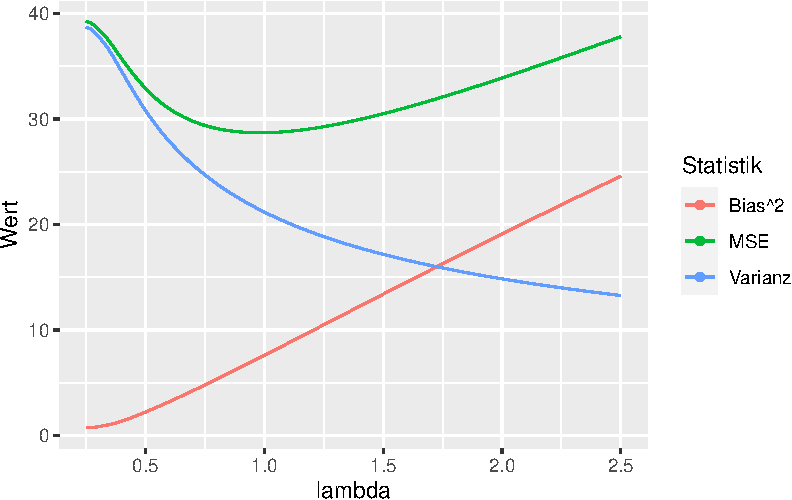
\includegraphics{RegReg_files/figure-pdf/fig-MSEBVT-1.pdf}

}

}

\subcaption{\label{fig-MSEBVT-1}Ridge Regression}
\end{minipage}%
\newline
\begin{minipage}[t]{\linewidth}

{\centering 

\raisebox{-\height}{

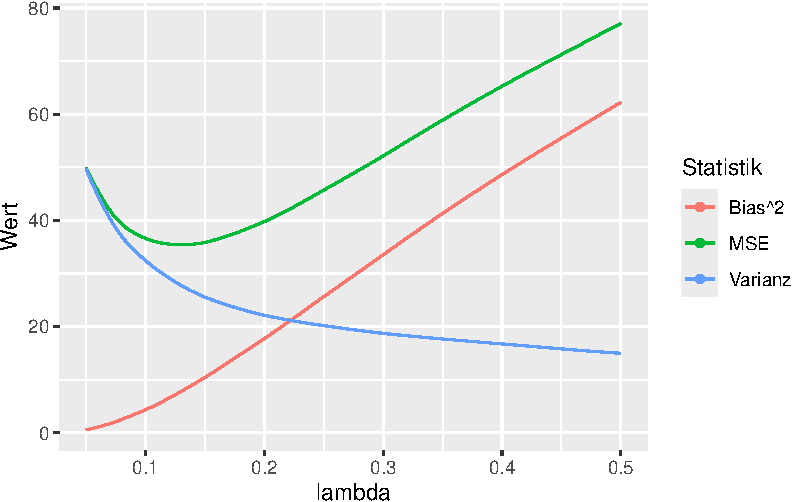
\includegraphics{RegReg_files/figure-pdf/fig-MSEBVT-2.pdf}

}

}

\subcaption{\label{fig-MSEBVT-2}Lasso Regression}
\end{minipage}%

\caption{\label{fig-MSEBVT}Simulierte MSE-Komponenten in Abhängigkeit
von Lambda}

\end{figure}

Anhand von Abbildung~\ref{fig-MSEBVT} lässt sich der
Bias-Variance-Tradeoff bei der Vorhersage von \(Y_0\) gut erkennen:
Bereits für kleine \(\lambda\) erzielen beide Methode eine deutliche
Reduktion des MSE. Dies wir durch etwas zusätzlichen Bias, aber eine
überproportionale Verringerung der Varianz erreicht. Der erkennbare
funktionale Zusammenhang zeigt, dass der MSE eine konvexe Funktion von
\(\lambda\) ist. Damit existieren optimale \(\lambda\) mit minimalem MSE
(grüne Punkte), die wir mit Cross Validation schätzen können.

\hypertarget{inferenz-fuxfcr-treatment-effekt-schuxe4tzung-mit-vielen-variablen}{%
\section{Inferenz für Treatment-Effekt-Schätzung mit vielen
Variablen}\label{inferenz-fuxfcr-treatment-effekt-schuxe4tzung-mit-vielen-variablen}}

In empirischen Studien des Effekts einer Behandlungsvariable \(B\) auf
eine Outcome-Variable \(Y\) steht häufig eine Vielzahl potentieller
Kontrollvariablen zur Verfügung. Häufig ist unklar, welche Variablen in
das Modell aufgenommen werden sollten, um das Risiko einer verzerrten
Schätzung durch ausgelassene Variablen zu vermindern und gleichzeitig
eine Schätzung mit geringer Varianz zu gewährleisten. Ist der
Beobachtungsumfang \(N\) relativ zur Variablenanzahl \(k\) groß, so kann
die KQ-Schätzung einer langen Regression (ein Modell mit allen \(k\)
Kontrollvariablen) gute Ergebnisse liefern. In der Praxis liegt diese
wünschenswerte Situation jedoch oft nicht vor und es ist \(k\lesssim N\)
oder sogar \(k>N\). Dann ist eine KQ-Schätzung des Behandlungseffekts
anhand aller \(k\) Variablen mit hoher Varianz behaftet bzw. gar nicht
möglich.\footnote{Beachte, dass der KQ-Schätzer bei \(k>N\) nicht lösbar
  ist.} Ein weiteres Szenario ist \(k(N)>N\), d.h. die Anzahl der
Regressoren kann mit dem Beobachtungsumfang wachsen.\footnote{Dieses
  Szenario wird unter Bedingungen bzgl. der Wachstumsrate und der Größe
  der Koeffizienten betrachet, s. (Belloni und Chernozhukov 2013).}
Lasso-Verfahren können dann hilfreich sein, um Determinanten von \(Y\)
\emph{und} \(B\) zu identifizieren und damit eine Menge an
Kontrollvariablen zu selektieren, für die eine erwartungstreue und
konsistente Schätzung des interessierenden Effekts wahrscheinlich ist.

Betrachte zunächst das Modell mit allen Kontrollvariablen \(X_j\),
\begin{align}
  Y_i = \beta_0 + \alpha_0 B_i + \sum_{j=1}^k \beta_{j} X_{i,j} + u_i, \label{eq:lassotmt}
\end{align} wobei einige \(\beta_{j}=0\) sind und wir annehmen, dass
\(B\) lediglich mit ein paar der \(X_j\) korrelliert. Die Shrinkage der
geschätzten Koeffizienten aus einer naiven Lasso-Regression von
\eqref{eq:lassotmt} führt grundsätzlich zu einer verzerrten Schätzung
des Behandlungseffekts \(\alpha_0\) und damit zu ungültiger
Inferenz.\footnote{Hahn u.~a. (2018) geben eine ausführliche Erläuterung
  dieser Problematik.}

Die Verzerrung von geschätzten Koeffizienten kann vermieden werden,
indem Lasso lediglich zur Selektion von Kontrollvariablen verwendet
wird. Dabei wird mit einer Lasso-Regression von \(Y\) auf die \(X_j\)
eine Teilmenge von Regressoren \(\mathcal{S}\) selektiert und der
Treatment-Effekt anschließend mit der KQ-Schätzung von \begin{align}
  Y_i = \beta_0 + \alpha_0 B_i + \sum_{j\in\mathcal{S}} \beta_{j} X_{i,j} + e_i,
\end{align} basierend auf der Selektion \(\mathcal{S}\) berechnet
wird.\footnote{Solche Verfahren werden \emph{Post-Selection-Schätzer}
  gennant.} Ein solcher \emph{Post-Lasso-Selection-Schätzer} (Belloni
und Chernozhukov 2013) ist jedoch im Allgemeinen und insbesondere in
hoch-dimensionalen Settings nicht konsistent für \(\alpha_0\) und nicht
asymptotisch normalverteilt, da weiterhin die Gefahr einer verzerrten
Schätzung durch in \(\mathcal{S}\) ausgelassene Variablen besteht, die
mit \(B\) korrelieren: Lasso selektiert Variablen \(X_j\), die ``gut''
\(Y\) erklären. Dabei kann nicht ausgeschlossen werden, das ein Modell
gewählt wird, dass relevante Determinanten von \(B\) auslässt. Selbst
wenn wir ein mit Lasso gewähltes Modell mit KQ (d.h. ohne Shrinkage)
schätzen, würde \(\alpha_0\) verzerrt geschätzt!

Belloni, Chernozhukov, und Hansen (2014) schlagen ein alternatives
Verfahren vor, dass auf Selektion der Determinanten \(X_j\) von \(Y\)
und \(B\) basiert. Dieses Verfahren wird als \emph{Post-Double
Selection} bezeichnet und kann wiefolgt implementiert werden:

\textbf{Post-Double-Selection-Schätzer}

\begin{enumerate}
\def\labelenumi{\arabic{enumi}.}
\item
  Bestimme die Determinanten \(X_j\) von \(Y\) mit Lasso-Regression und
  bezeichne die Menge der selektierten Variablen als \(\mathcal{S}_Y\).
\item
  Bestimme die Determinanten \(X_j\) von \(B\) mit Lasso-Regression und
  bezeichne die Menge der selektierten Variablen als \(\mathcal{S}_B\).
\item
  Bestimme die Schnittmenge
  \(\mathcal{S}_{YB} = \mathcal{S}_Y \cap \mathcal{S}_B\). Schätze den
  Treatment-Effekt als \(\widehat{\alpha}_0\) in der KQ-Regression
  \begin{align}
    Y_i = \beta_0 + \alpha_0 B_i + \sum_{j\in\mathcal{S}_{YB}} \beta_{j} X_{i,j} + v_i.
  \end{align}
\end{enumerate}

Belloni, Chernozhukov, und Hansen (2014) zeigen, dass
\(\widehat{\alpha}_0\) aus diesem Verfahren ein asymptotisch
normalverteiler Schätzer für \(\alpha_0\) ist und herkömmliche t-Tests
und Konfidenzintervalle gültige Inferenz erlauben.

Wir illustrieren die in diesem Abschnitt betrachteten Schätzer nun
anhand simulierter Daten mit R. Die fiktive Problemstellung ist die
Schätzung eines wahren Treatment-Effekts \(\alpha_0 = 2\), wenn so viele
potenzielle Kontrollvariablen vorliegen, dass der KQ-Schätzer gerade
noch berechnet werden kann, aber aufgrund hoher Varianz unzuverlässig
ist. Hierzu erzeugen wir \(Y\) gemäß der Vorschrift \begin{align*}
  Y_i =&\, \alpha_0 B_i + \sum_{j=1}^{k_Y} \beta_{j}^Y X_{i,j}^Y + \sum_{l=1}^{k_{YB}} \beta_{l}^{YB} X_{i,l}^{YB} + u_i,\\
  \\
  \beta_j^{YB} \overset{u.i.v}{\sim}&\,N(10,1), \quad \beta_j^{Y} \overset{u.i.v}{\sim}U(0,1), \quad u_i \overset{u.i.v}{\sim}N(0,1).\\
  \\
  i=&\,1,\dots,550
\end{align*}

Die Behandlungsvariable \(B_i\) entspricht der Vorschrift \begin{align*}
  B_i =&\, \sum_{l=1}^{k_{YB}} \beta_{l}^{YB} X_{i,l}^{YB} + e_i,\\
  \\
  \beta_j^{YB} \overset{u.i.v}{\sim}&\,N(2,0.2), \quad e_i \overset{u.i.v}{\sim}N(0,1).
\end{align*} Wir wählen \(k_{YB} = k_{Y} = 25\). Zusätzlich zu \(B\),
den Determinanten von \(Y\) \emph{und} \(B\) (\(X^{YB}\)) sowie den
Variablen, die ausschließlich \(Y\) beeinflussen (\(X^{Y}\)) gibt es
\(k_U = 499\) Variablen \(X^U\), die weder \(Y\) noch \(B\) beeinflussen
und damit irrelevant für die Schätzung des Behandlungseffekts sind. Wir
haben also \(N=550\) Beobachtungen und insgesamt
\(k = 1+k_{Y} + k_{YB} + k_{U} = 550\) potenzielle Kontrollvariablen von
denen \(k_{YB} = 25\) für eine unverzerrte Schätzung von \(\alpha_0\)
relevant sind.

Der nachstehende Code generiert die Daten gemäß der Vorschrift.

\begin{Shaded}
\begin{Highlighting}[]
\FunctionTok{library}\NormalTok{(mvtnorm)}
\FunctionTok{library}\NormalTok{(tidyverse)}
\FunctionTok{set.seed}\NormalTok{(}\DecValTok{4321}\NormalTok{)}

\NormalTok{n }\OtherTok{\textless{}{-}} \DecValTok{550}      \CommentTok{\# Beobachtungen}
\NormalTok{p\_Y }\OtherTok{\textless{}{-}} \DecValTok{25}     \CommentTok{\# Determinanten Y}
\NormalTok{p\_B }\OtherTok{\textless{}{-}} \DecValTok{25}     \CommentTok{\# Determinanten B *und* Y}
\NormalTok{p\_U }\OtherTok{\textless{}{-}} \DecValTok{499}    \CommentTok{\# irrelevante Variablen }

\CommentTok{\# Variablen generieren}
\NormalTok{XB }\OtherTok{\textless{}{-}} \FunctionTok{rmvnorm}\NormalTok{(}\AttributeTok{n =}\NormalTok{ n, }\AttributeTok{sigma =} \FunctionTok{diag}\NormalTok{(p\_B))}
\NormalTok{XU }\OtherTok{\textless{}{-}} \FunctionTok{rmvnorm}\NormalTok{(}\AttributeTok{n =}\NormalTok{ n, }\AttributeTok{sigma =} \FunctionTok{diag}\NormalTok{(p\_U))}
\NormalTok{XY }\OtherTok{\textless{}{-}} \FunctionTok{rmvnorm}\NormalTok{(}\AttributeTok{n =}\NormalTok{ n, }\AttributeTok{sigma =} \FunctionTok{diag}\NormalTok{(p\_Y))}

\CommentTok{\# Stetige Behandlungsvariable erzeugen}
\NormalTok{B }\OtherTok{\textless{}{-}}\NormalTok{ XB }\SpecialCharTok{\%*\%} \FunctionTok{rnorm}\NormalTok{(p\_B, }\DecValTok{2}\NormalTok{, }\AttributeTok{sd =}\NormalTok{ .}\DecValTok{2}\NormalTok{) }\SpecialCharTok{+} \FunctionTok{rnorm}\NormalTok{(n)}

\CommentTok{\# Abh. Variable erzeugen, Behandlungseffekt (ATE) ist 2}
\NormalTok{Y }\OtherTok{\textless{}{-}} \DecValTok{2} \SpecialCharTok{*}\NormalTok{ B }\SpecialCharTok{+} 
\NormalTok{  XB }\SpecialCharTok{\%*\%} \FunctionTok{rnorm}\NormalTok{(p\_B, }\AttributeTok{mean =} \DecValTok{10}\NormalTok{) }\SpecialCharTok{+} 
\NormalTok{  XY }\SpecialCharTok{\%*\%} \FunctionTok{runif}\NormalTok{(p\_Y) }\SpecialCharTok{+} 
  \FunctionTok{rnorm}\NormalTok{(n)}

\CommentTok{\# Variablen in tibble sammeln}
\NormalTok{X }\OtherTok{\textless{}{-}} \FunctionTok{cbind}\NormalTok{(B, XB, XU, XY) }\SpecialCharTok{\%\textgreater{}\%} 
  \FunctionTok{as\_tibble}\NormalTok{()}

\CommentTok{\# Namen zuweisen}
\FunctionTok{colnames}\NormalTok{(X) }\OtherTok{\textless{}{-}} \FunctionTok{c}\NormalTok{(}
  \StringTok{"B"}\NormalTok{, }
  \FunctionTok{paste0}\NormalTok{(}\StringTok{"XB"}\NormalTok{, }\DecValTok{1}\SpecialCharTok{:}\NormalTok{p\_B), }
  \FunctionTok{paste0}\NormalTok{(}\StringTok{"XU"}\NormalTok{, }\DecValTok{1}\SpecialCharTok{:}\NormalTok{p\_U),}
  \FunctionTok{paste0}\NormalTok{(}\StringTok{"XY"}\NormalTok{, }\DecValTok{1}\SpecialCharTok{:}\NormalTok{p\_Y) }
\NormalTok{)}
\end{Highlighting}
\end{Shaded}

Wünschenswert wäre die KQ-Schätzung des wahren Modells. Diese ergibt
eine Schätzung nahe des wahren Treatment-Effekts \(\alpha_0 = 2\). Unter
realen Bedingungen wäre diese Regression jedoch nicht implementierbar,
weil die relevanten Kovariablen \texttt{XB} unbekannt sind.

\begin{Shaded}
\begin{Highlighting}[]
\CommentTok{\# KQ: Wahres Modell schätzen}
\FunctionTok{lm}\NormalTok{(Y }\SpecialCharTok{\textasciitilde{}}\NormalTok{ B }\SpecialCharTok{+}\NormalTok{ XB }\SpecialCharTok{{-}} \DecValTok{1}\NormalTok{)}\SpecialCharTok{$}\NormalTok{coefficients[}\StringTok{"B"}\NormalTok{]}
\end{Highlighting}
\end{Shaded}

\begin{verbatim}
       B 
1.937031 
\end{verbatim}

Wir schätzen daher zunächst die ``lange'' Regression mit allen \(k\)
verfügbaren Variablen mit KQ. Beachte, dass der KQ-Schätzer für
\(\alpha_0\) zwar implementierbar und erwartungstreu ist, jedoch eine
hohe Varianz aufweist. Wegen \(k=N=550\) erhalten wir eine perfekte
Anpassung an die Daten und können mangels Freiheitsgraden keine
Hypothesentests durchführen.

\begin{Shaded}
\begin{Highlighting}[]
\CommentTok{\# KQ: Lange Regression schätzen}
\FunctionTok{lm}\NormalTok{(Y }\SpecialCharTok{\textasciitilde{}}\NormalTok{ . }\SpecialCharTok{{-}} \DecValTok{1}\NormalTok{, }\AttributeTok{data =}\NormalTok{ X)}\SpecialCharTok{$}\NormalTok{coefficients[}\StringTok{"B"}\NormalTok{]}
\end{Highlighting}
\end{Shaded}

\begin{verbatim}
       B 
3.079497 
\end{verbatim}

Die KQ-Schätzung von \(\alpha_0\) anhand der langen Regression weicht
deutlich vom wahren Wert \(\alpha_0 = 2\) ab.

Eine ``kurze'' KQ-Regression nur mit der Behandlungsvariable \(B\) führt
wegen Korrelation mit den ausgelassenen Determinanten in \texttt{XB} zu
einer deutlich verzerrten Schätzung.

\begin{Shaded}
\begin{Highlighting}[]
\CommentTok{\# KQ: Kurze Regression}
\FunctionTok{lm}\NormalTok{(Y }\SpecialCharTok{\textasciitilde{}}\NormalTok{ B }\SpecialCharTok{{-}} \DecValTok{1}\NormalTok{)}\SpecialCharTok{$}\NormalTok{coefficients[}\StringTok{"B"}\NormalTok{]}
\end{Highlighting}
\end{Shaded}

\begin{verbatim}
       B 
6.716837 
\end{verbatim}

Die Methoden von Belloni und Chernozhukov (2013) und Belloni,
Chernozhukov, und Hansen (2014) sind im R-Paket \texttt{hdm}
implementiert. Mit den Funktionen \texttt{hrm::rlasso()} und
\texttt{hdm::rlassoEffect} kann Lasso-Regression sowie Post- und
Double-Post-Selection durchgeführt werden.\footnote{Diese Funktionen
  ermitteln ein optimales \(\lambda\) mit dem in Belloni u.~a. (2012)
  vorgeschlagenen Algorithmus.}

Wir berechnen zunächst den naiven Lasso-Schätzer in einem Modell mit
allen Variablen.

\begin{Shaded}
\begin{Highlighting}[]
\FunctionTok{library}\NormalTok{(hdm)}

\CommentTok{\# Naiver Post{-}Lasso{-}Schätzer}
\NormalTok{lasso }\OtherTok{\textless{}{-}} \FunctionTok{rlasso}\NormalTok{(}
  \AttributeTok{x =}\NormalTok{ X, }
  \AttributeTok{y =}\NormalTok{ Y, }
  \AttributeTok{intercept =}\NormalTok{ F, }
  \AttributeTok{post =}\NormalTok{ F}
\NormalTok{)}

\CommentTok{\# Koeffizientenschätzer auslesen}
\NormalTok{lasso}\SpecialCharTok{$}\NormalTok{coefficients[}\StringTok{"B"}\NormalTok{] }
\end{Highlighting}
\end{Shaded}

\begin{verbatim}
       B 
6.368456 
\end{verbatim}

Auch dieser Schätzer ist deutlich verzerrt. Problematisch ist hier nicht
nur die Shrinkage auf \(\widehat{\alpha}_0\), sondern die Selektion der
Variablen in \texttt{XB}:

\begin{Shaded}
\begin{Highlighting}[]
\CommentTok{\# Welche Variablen in XB selektiert Lasso *nicht*?}
\NormalTok{nselektiert }\OtherTok{\textless{}{-}} \FunctionTok{which}\NormalTok{(lasso}\SpecialCharTok{$}\NormalTok{coef[}\DecValTok{1}\SpecialCharTok{:}\DecValTok{26}\NormalTok{] }\SpecialCharTok{==} \DecValTok{0}\NormalTok{)   }\CommentTok{\# ID}

\CommentTok{\# Namen auslesen}
\FunctionTok{names}\NormalTok{(lasso}\SpecialCharTok{$}\NormalTok{coef[}\DecValTok{1}\SpecialCharTok{:}\DecValTok{26}\NormalTok{])[nselektiert]}
\end{Highlighting}
\end{Shaded}

\begin{verbatim}
[1] "XB8"  "XB10" "XB16" "XB18" "XB20"
\end{verbatim}

Durch das Auslassen dieser Determinanten von \(Y\) und \(B\) leidet der
Lasso-Schätzer unter OVB.

Als nächstes berechnen wir den Post-Lasso-Selection-Schätzer.

\begin{Shaded}
\begin{Highlighting}[]
\CommentTok{\# Post{-}Lasso{-}Selection{-}Schätzer berechnen}
\NormalTok{p\_lasso }\OtherTok{\textless{}{-}} \FunctionTok{rlasso}\NormalTok{(}
  \AttributeTok{x =}\NormalTok{ X,}
  \AttributeTok{y =}\NormalTok{ Y, }
  \AttributeTok{intercept =}\NormalTok{ F, }
  \AttributeTok{post =}\NormalTok{ T}
\NormalTok{)}

\CommentTok{\# Schätzung für alpha\_0}
\NormalTok{p\_lasso}\SpecialCharTok{$}\NormalTok{coef[}\StringTok{"B"}\NormalTok{]}
\end{Highlighting}
\end{Shaded}

\begin{verbatim}
       B 
6.362409 
\end{verbatim}

Die Ähnlichkeit der Post-Lasso-Schätzung von \(\alpha_0\) zur
Lasso-Schätzung zeigt deutlich, dass die Verzerrung des Lasso-Schätzers
überwiegend durch ausgelassene Variablen anstatt durch Shrinkage
verursacht wird.

Mit \texttt{rlassoEffect()} können wir den
Post-Double-Selection-Schätzer berechnen.

\begin{Shaded}
\begin{Highlighting}[]
\CommentTok{\# Post{-}Double{-}Selection{-}Schätzer}
\NormalTok{pds\_lasso }\OtherTok{\textless{}{-}} \FunctionTok{rlassoEffect}\NormalTok{(}
  \AttributeTok{x =}\NormalTok{ X }\SpecialCharTok{\%\textgreater{}\%} 
\NormalTok{    dplyr}\SpecialCharTok{::}\FunctionTok{select}\NormalTok{(}\SpecialCharTok{{-}}\NormalTok{B) }\SpecialCharTok{\%\textgreater{}\%} 
    \FunctionTok{as.matrix}\NormalTok{(),}
  \AttributeTok{y =}\NormalTok{ Y, }
  \AttributeTok{d =}\NormalTok{ B, }
  \AttributeTok{method =} \StringTok{"double selection"}
\NormalTok{)}

\CommentTok{\# Schnittmenge der selektierten Determinanten }
\CommentTok{\# von Y und B}
\NormalTok{(}
\NormalTok{  S\_BY }\OtherTok{\textless{}{-}} \FunctionTok{names}\NormalTok{(}
    \FunctionTok{which}\NormalTok{(pds\_lasso}\SpecialCharTok{$}\NormalTok{selection.index)}
\NormalTok{  )}
\NormalTok{)}
\end{Highlighting}
\end{Shaded}

\begin{verbatim}
 [1] "XB1"   "XB2"   "XB3"   "XB4"   "XB5"   "XB6"   "XB7"   "XB8"   "XB9"  
[10] "XB10"  "XB11"  "XB12"  "XB13"  "XB14"  "XB15"  "XB16"  "XB17"  "XB18" 
[19] "XB19"  "XB20"  "XB21"  "XB22"  "XB23"  "XB24"  "XB25"  "XU209" "XU241"
[28] "XU295" "XY3"   "XY7"   "XY8"   "XY12"  "XY13"  "XY15"  "XY16"  "XY19" 
[37] "XY23" 
\end{verbatim}

Double Selection führt ebenfalls zu einem Post-Lasso-KQ-Schätzer mit
allen 25 relevaten Variablen in \texttt{XB}. Wir selektieren allerdings
deutlich weniger irrelevante Variablen aus \texttt{XU} als mit Single
Selection und dennoch einige Determinanten von \(Y\) aus \texttt{XY}.
Double Selection führt also zu einer unverzerrten Schätzen mit
geringerer Varianz. Mit \texttt{summary()} erhalten wir gültige Inferenz
bzgl. des Treatment-Effekts.

\begin{Shaded}
\begin{Highlighting}[]
\FunctionTok{summary}\NormalTok{(pds\_lasso)}
\end{Highlighting}
\end{Shaded}

\begin{verbatim}
[1] "Estimates and significance testing of the effect of target variables"
   Estimate. Std. Error t value Pr(>|t|)    
d1   1.94977    0.07127   27.36   <2e-16 ***
---
Signif. codes:  0 '***' 0.001 '**' 0.01 '*' 0.05 '.' 0.1 ' ' 1
\end{verbatim}

Der Post-Double-Selection-Schätzer liefert unter den betrachteten
Verfahren die beste Schätzung von \(\alpha_0\) und erlaubt gülstige
statistische Inferenz. Der geschätzte Effekt ist hoch-signifikant.

\begin{tcolorbox}[enhanced jigsaw, colbacktitle=quarto-callout-note-color!10!white, bottomtitle=1mm, breakable, leftrule=.75mm, opacityback=0, title=\textcolor{quarto-callout-note-color}{\faInfo}\hspace{0.5em}{Key Facts zum Post-Double-Selection-Schätzer}, left=2mm, arc=.35mm, titlerule=0mm, bottomrule=.15mm, opacitybacktitle=0.6, coltitle=black, toptitle=1mm, colback=white, colframe=quarto-callout-note-color-frame, toprule=.15mm, rightrule=.15mm]

\begin{itemize}
\item
  Durch die sorgfältige Auswahl von Variablen, die mit Behandlung- und
  Outcome-Variable zusammenhängen, ermöglicht die Double-Selection eine
  bessere Kontrolle über das Risiko ausgelassender Variablen in
  Beobachtungsstudien und ermöglicht gültige (asymptotisch normale)
  Inferenz.
\item
  Der Post-Double-Selection-Schätzer besteht aus drei Regressionen:

  \begin{enumerate}
  \def\labelenumi{\arabic{enumi}.}
  \tightlist
  \item
    Es werden Variablen mit Lasso selektiert, welche die
    \emph{Behandlungs-Variable} erklären.
  \item
    Es werden Variablen mit Lasso selektiert, welche die
    \emph{Outcome-Variable} erklären.
  \item
    Der Post-Double-Selection-Schätzer ist der KQ-Schätzer in einer
    Regression, die für die Schnittmenge der ausgewählten Variablen
    kontrolliert.
  \end{enumerate}
\item
  Dank der Selektion mit Lasso kann der Schätzer auch bei
  hoch-dimensionalen Daten (\(k>n\)) angewendet werden.
\item
  Post-Double-Selection-Schätzer für Behandlungseffekte sind im R-Paket
  \texttt{hdm} implementiert.
\end{itemize}

\end{tcolorbox}

\hypertarget{case-study-makrouxf6konomisches-wachstum}{%
\subsection{Case Study: Makroökonomisches
Wachstum}\label{case-study-makrouxf6konomisches-wachstum}}

Zur Illustration des Post-Double-Selection Schätzers betrachten wir eine
empirische Anwendung bzgl. der Validierung von makroökonomischer
Wachstumtheorie. Aus neo-klassischen Ansätzen wie dem
\href{https://de.wikipedia.org/wiki/Solow-Modell}{Solow-Swan-Modell}
kann die Hypothese, dass Volkswirtschaften zu einem gemeinsamen
Wachstumspfad hin konvergieren, abgeleitet werden. Diese
Konvergenzhypothese impliziert die Existenz von Aufholeffekten: Ärmere
Volkswirtschaften müssen im mittel schneller Wachsen als die Wirschaft
wohlhabender Länder. Die grundlegende Spezifikation eines entsprechenden
Regressionsmodells lautet \begin{align}
  \text{WR}_{i} = \alpha_0 \text{BIP0}_i + u_i, \label{eq:growthmodel1}
\end{align} wobei \(\text{WR}_{i}\) die Wachstumsrate des Pro-Kopf-BIP
in Land \(i\) über einen Zeitraum (typischerweise berechnet als
Log-Differenz zwischen zwei Perioden) und \(\text{BIP0}_i\) das
(logarithmierte) Pro-Kopf-BIP zu beginn der Referenzperiode ist. Gemäß
der Konvergenzhypothese muss \(\alpha_0<0\) sein: Je wohlhabender eine
Volkswirtschaft ist, desto geringer ist das Wirtschaftswachstum.

Um Verzerrung durch ausgelassene Kovariablen zu vermeiden, sollte das
Modell \eqref{eq:growthmodel1} um länder-spezifische Regressoren
\(x_{i,j}\), die sowohl das Ausgagnsniveau \(\text{BIP0}\) sowie die
Wachtumsrate beinflussen, erweitert werden. Zu der großen Menge
potentieller Kovariablen gehören makro- und sozio-ökonomische Maße wie
bspw. die Investitionstätigkeit des Staates, Offenheit der
Volkswirtschaft, das politische Umfeld, das Bildungsniveau, die
Demographie usw. Eine bevorzugte Spezifikation ist daher \begin{align}
  \text{WR}_{i} = \alpha_0 \text{BIP0}_i + \sum_{j=1}^k \beta_j x_{i,j} + u_i,\label{eq:growthmodel2}
\end{align} wobei \(\alpha_0\) als Behandlungseffekt interpretiert
werden kann. Beachte, dass \eqref{eq:growthmodel2} eine Regression in
der Form von \eqref{eq:lassotmt} ist.

Wir illustrieren die Schätzung von und Inferenz bzgl. \(\alpha_0\) in
\eqref{eq:growthmodel2} mit Post-Double-Selektion für einen 90 Länder
umfassenden Auszug aus dem Datensatz von Barro und Lee (2013), der als
Objekt \texttt{GrowthData} im R-Paket \texttt{hdm} verfügbar
ist.\footnote{Eine ausführliche Beschreibung der Variablen ist
  \href{https://www2.nber.org/pub/barro.lee/readme.txt}{hier} einsehbar.}

\begin{Shaded}
\begin{Highlighting}[]
\CommentTok{\# Datensatz in Arbeitsumgebung verfügbar machen}
\FunctionTok{library}\NormalTok{(hdm)}
\FunctionTok{data}\NormalTok{(GrowthData)}

\CommentTok{\# Anzahl Beobachtungen und Variablen}
\FunctionTok{dim}\NormalTok{(GrowthData)}
\end{Highlighting}
\end{Shaded}

\begin{verbatim}
[1] 90 63
\end{verbatim}

Die Spalte \texttt{Outcome} ist die jeweilige Wachstumsrate des BIP
zwischen den Perioden 1965-1975 und 1975-1985 und \texttt{gdpsh465} ist
das reale Pro-Kopf-BIP im Jahr 1965 zu Preisen von 1980.

Wir führen zunächst eine graphische Analyse hinsichtlich des Modells
einfachen Modells \eqref{eq:growthmodel1} durch, indem wir
\texttt{gdpsh465} gegen \texttt{Outcome} plotten und die geschätzte
Regressionsgerade einzeichnen.

\begin{Shaded}
\begin{Highlighting}[]
\CommentTok{\# Einfache grafische Analyse mit ggplot2}
\NormalTok{GrowthData }\SpecialCharTok{\%\textgreater{}\%}
  \FunctionTok{ggplot}\NormalTok{(}
    \AttributeTok{mapping =} \FunctionTok{aes}\NormalTok{(}
      \AttributeTok{x =}\NormalTok{ gdpsh465, }
      \AttributeTok{y =}\NormalTok{ Outcome}
\NormalTok{    )}
\NormalTok{  ) }\SpecialCharTok{+}
  \FunctionTok{geom\_point}\NormalTok{() }\SpecialCharTok{+}
  \FunctionTok{geom\_smooth}\NormalTok{(}\AttributeTok{method =} \StringTok{"lm"}\NormalTok{, }\AttributeTok{se =}\NormalTok{ F)}
\end{Highlighting}
\end{Shaded}

\begin{figure}[t]

{\centering 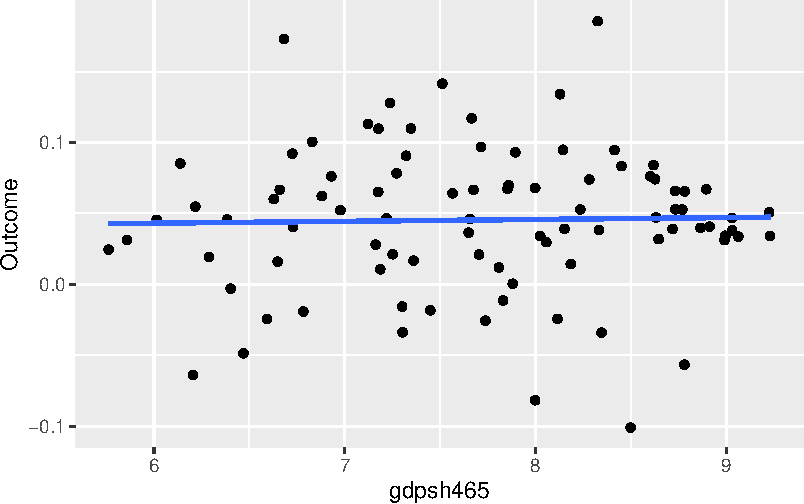
\includegraphics{RegReg_files/figure-pdf/fig-bipsimple-1.pdf}

}

\caption{\label{fig-bipsimple}BIP-Wachstum: Einfache Regression}

\end{figure}

Abbildung~\ref{fig-bipsimple} zeigt einen geringen positiven geschätzten
Effekt \(\widehat{\alpha}_0\). Eine Auswertung mit \texttt{lm()} ergibt,
dass der Effekt \(\alpha_0\) nicht signifikant von \(0\) verschieden
ist.

\begin{Shaded}
\begin{Highlighting}[]
\CommentTok{\# Einfache Regression durchführen, }
\CommentTok{\# Inferenz für gdpsh465 erhalten}
\FunctionTok{lm}\NormalTok{(Outcome }\SpecialCharTok{\textasciitilde{}}\NormalTok{ gdpsh465, }\AttributeTok{data =}\NormalTok{ GrowthData) }\SpecialCharTok{\%\textgreater{}\%}
  \FunctionTok{summary}\NormalTok{() }\SpecialCharTok{\%\textgreater{}\%}
  \FunctionTok{coefficients}\NormalTok{() }\SpecialCharTok{\%\textgreater{}\%} 
\NormalTok{  .[}\DecValTok{2}\NormalTok{, ]}
\end{Highlighting}
\end{Shaded}

\begin{verbatim}
   Estimate  Std. Error     t value    Pr(>|t|) 
0.001316713 0.006102200 0.215776701 0.829661165 
\end{verbatim}

Der positive Effekt aus der einfachen Schätzung widerspricht der
Konvergenzhypothese. Dieses Ergebnis könnte allerdings durch Auslassen
relevanter Kovariablen ungültig sein. Beispielsweise ist es plausibel,
dass das Bildungsniveau einer Volkswirtschaft sowohl mit dem BIP
korreliert ist als auch die Wachstumsrate beeinflusst. Dann wäre das
Bildungsniveau eine relevante Kovariable, deren Auslassen zu einer
verzerrten Schätzung von \(\alpha_0\) führt.

Eine ``lange'' Regression mit allen Kovariablen ist zwar möglich, aber
problematisch: Das Verhältnis von Beobachtungen (90) zu Regressoren (62)
bedeutet eine hohe Unsicherheit der Schätzung.

\begin{Shaded}
\begin{Highlighting}[]
\CommentTok{\# Inferenz für alpha\_0 in langer Regression}
\FunctionTok{summary}\NormalTok{(}
  \FunctionTok{lm}\NormalTok{(Outcome }\SpecialCharTok{\textasciitilde{}}\NormalTok{ . }\SpecialCharTok{{-}} \DecValTok{1}\NormalTok{ , }\AttributeTok{data =}\NormalTok{ GrowthData)}
\NormalTok{  ) }\SpecialCharTok{\%\textgreater{}\%} 
  \FunctionTok{coefficients}\NormalTok{() }\SpecialCharTok{\%\textgreater{}\%} 
\NormalTok{  .[}\DecValTok{2}\NormalTok{, ]}
\end{Highlighting}
\end{Shaded}

\begin{verbatim}
    Estimate   Std. Error      t value     Pr(>|t|) 
-0.009377989  0.029887726 -0.313773911  0.756018518 
\end{verbatim}

Der geschätzte Koeffizient \(\widehat{\alpha}_0\) ist nun zwar negativ,
liefert jedoch weiterhin keine Evidenz, dass \(\alpha_0\) von 0
verschieden ist. Ein Vergleich der Standardfehler zeigt aber, dass die
KQ-Schätzung aufgrund Berücksichtigung aller potentiellen Kovariablen
mit deutlich größerer Varianz behaftet ist als in der einfachen
KQ-Regression \eqref{eq:growthmodel1}

Post-Double-Selection erlaubt gültige Inferenz bzgl. \(\alpha_0\) nach
Schätzung der Menge relevanter Kovariablen. Wir weisen die
entsprechenden Variablen R-Objekten zu und berechnen den Schätzer.

\begin{Shaded}
\begin{Highlighting}[]
\CommentTok{\# Variablen für Post{-}Double{-}Selection vorbereiten}

\CommentTok{\# abh. Variable}
\NormalTok{y }\OtherTok{\textless{}{-}}\NormalTok{ GrowthData }\SpecialCharTok{\%\textgreater{}\%} 
  \FunctionTok{pull}\NormalTok{(Outcome)}

\CommentTok{\# "Treatment"}
\NormalTok{d }\OtherTok{\textless{}{-}}\NormalTok{ GrowthData }\SpecialCharTok{\%\textgreater{}\%} 
  \FunctionTok{pull}\NormalTok{(gdpsh465)}

\CommentTok{\# potentielle Regressoren}
\NormalTok{X }\OtherTok{\textless{}{-}}\NormalTok{ GrowthData }\SpecialCharTok{\%\textgreater{}\%} 
\NormalTok{  dplyr}\SpecialCharTok{::}\FunctionTok{select}\NormalTok{(}
    \SpecialCharTok{{-}}\NormalTok{Outcome, }\SpecialCharTok{{-}}\NormalTok{intercept, }\SpecialCharTok{{-}}\NormalTok{gdpsh465}
\NormalTok{  )}
\end{Highlighting}
\end{Shaded}

\begin{Shaded}
\begin{Highlighting}[]
\CommentTok{\# Post{-}Double{-}Selection{-}Schätzer berechnen}
\NormalTok{Growth\_DS }\OtherTok{\textless{}{-}} 
  \FunctionTok{rlassoEffect}\NormalTok{(}
    \AttributeTok{x =}\NormalTok{ X }\SpecialCharTok{\%\textgreater{}\%} 
      \FunctionTok{as.matrix}\NormalTok{(), }
    \AttributeTok{y =}\NormalTok{ y, }
    \AttributeTok{d =}\NormalTok{ d, }
    \AttributeTok{method =} \StringTok{"double selection"}
\NormalTok{)}
\end{Highlighting}
\end{Shaded}

Post-Double-Selection wählt aus der Menge potentieller Kovariablen
lediglich sieben Regressoren aus.

\begin{Shaded}
\begin{Highlighting}[]
\CommentTok{\# Selektierte Variablen einsehen}
\CommentTok{\# ID}
\NormalTok{Selektion }\OtherTok{\textless{}{-}}\NormalTok{ Growth\_DS}\SpecialCharTok{$}\NormalTok{selection.index}

\CommentTok{\# Namen auslesen}
\FunctionTok{names}\NormalTok{(}
  \FunctionTok{which}\NormalTok{(Selektion }\SpecialCharTok{==}\NormalTok{ T)}
\NormalTok{)}
\end{Highlighting}
\end{Shaded}

\begin{verbatim}
[1] "bmp1l"    "freetar"  "hm65"     "sf65"     "lifee065" "humanf65" "pop6565" 
\end{verbatim}

Tabelle~\ref{tbl-growthpdssek} zeigt die Definitionen der ausgewählten
Variablen.

\hypertarget{tbl-growthpdssek}{}
\begin{longtable}{ll}
\caption{\label{tbl-growthpdssek}Mit PDS selektierte Variablen aus \texttt{GrowthData}. Referenzjahr
1965. }\tabularnewline

\toprule
Variable & Beschreibung \\ 
\midrule\addlinespace[2.5pt]
bmp1l & Schwarzmarktprämie d. Währung \\ 
freetar & Maß für Zollbeschränkungen \\ 
hm65 & Einschreibungsquote Uni (Männer)  \\ 
sf65 & Beschulungsquote Sekundarstufe (Frauen) \\ 
lifee065 & Lebenserwartung bei Geburt \\ 
humanf65 & Durschn. Bildung im Alter 25 (Frauen) \\ 
pop6565 & Anteil Bevölkerung ü. 65 Jahre \\ 
\bottomrule
\end{longtable}

\begin{Shaded}
\begin{Highlighting}[]
\CommentTok{\# Gültige Inferenz mit dem Post{-}Double{-}Selection{-}Schätzer}
\FunctionTok{summary}\NormalTok{(Growth\_DS)}
\end{Highlighting}
\end{Shaded}

\begin{verbatim}
[1] "Estimates and significance testing of the effect of target variables"
   Estimate. Std. Error t value Pr(>|t|)   
d1  -0.05001    0.01579  -3.167  0.00154 **
---
Signif. codes:  0 '***' 0.001 '**' 0.01 '*' 0.05 '.' 0.1 ' ' 1
\end{verbatim}

Das Ergebnis der Post-Double-Selection-Schätzung unterstützt die
(bedingte) Konvergenzhypothese mit einer signifikanten negativen
Schätzung \(\widehat{\alpha}_0\approx-0.05\).

\bookmarksetup{startatroot}

\hypertarget{literatur-1}{%
\chapter*{Literatur}\label{literatur-1}}
\addcontentsline{toc}{chapter}{Literatur}

\markboth{Literatur}{Literatur}

\hypertarget{refs}{}
\begin{CSLReferences}{1}{0}
\leavevmode\vadjust pre{\hypertarget{ref-BarroLee2013}{}}%
Barro, Robert J., und Jong Wha Lee. 2013. {„A new data set of
educational attainment in the world, 1950--2010``}. \emph{Journal of
Development Economics} 104: 184--98.
https://doi.org/\url{https://doi.org/10.1016/j.jdeveco.2012.10.001}.

\leavevmode\vadjust pre{\hypertarget{ref-BastenBetz2013}{}}%
Basten, Christoph, und Frank Betz. 2013. {„Beyond work ethic: Religion,
individual, and political preferences``}. \emph{American Economic
Journal: Economic Policy} 5 (3): 67--91.

\leavevmode\vadjust pre{\hypertarget{ref-Bellonietal2012}{}}%
Belloni, Alexandre, Daniel Chen, Victor Chernozhukov, und Christian
Hansen. 2012. {„Sparse models and methods for optimal instruments with
an application to eminent domain``}. \emph{Econometrica} 80 (6):
2369--429.

\leavevmode\vadjust pre{\hypertarget{ref-BelloniChernozhukov2013}{}}%
Belloni, Alexandre, und Victor Chernozhukov. 2013. {„Least squares after
model selection in high-dimensional sparse models``}. \emph{Bernoulli},
521--47.

\leavevmode\vadjust pre{\hypertarget{ref-Bellonietal2014}{}}%
Belloni, Alexandre, Victor Chernozhukov, und Christian Hansen. 2014.
{„High-dimensional methods and inference on structural and treatment
effects``}. \emph{Journal of Economic Perspectives} 28 (2): 29--50.

\leavevmode\vadjust pre{\hypertarget{ref-CJM2020}{}}%
Cattaneo, Matias D, Michael Jansson, und Xinwei Ma. 2020. {„Simple local
polynomial density estimators``}. \emph{Journal of the American
Statistical Association} 115 (531): 1449--55.

\leavevmode\vadjust pre{\hypertarget{ref-CortezSilva2008}{}}%
Cortez, Paulo, und Alice Maria Gonçalves Silva. 2008. {„Using data
mining to predict secondary school student performance``}.

\leavevmode\vadjust pre{\hypertarget{ref-Efronetal2004}{}}%
Efron, Bradley, Trevor Hastie, Iain Johnstone, und Robert Tibshirani.
2004. {„Least angle regression``}.

\leavevmode\vadjust pre{\hypertarget{ref-GelmanImbens2019}{}}%
Gelman, Andrew, und Guido Imbens. 2019. {„Why high-order polynomials
should not be used in regression discontinuity designs``}. \emph{Journal
of Business \& Economic Statistics} 37 (3): 447--56.

\leavevmode\vadjust pre{\hypertarget{ref-Hahnetal2018}{}}%
Hahn, P Richard, Carlos M Carvalho, David Puelz, und Jingyu He. 2018.
{„Regularization and confounding in linear regression for treatment
effect estimation``}.

\leavevmode\vadjust pre{\hypertarget{ref-HoerlKennard1970}{}}%
Hoerl, Arthur E, und Robert W Kennard. 1970. {„{Ridge regression: Biased
estimation for nonorthogonal problems}``}. \emph{Technometrics} 12 (1):
55--67.

\leavevmode\vadjust pre{\hypertarget{ref-ImbensLemieux2008}{}}%
Imbens, G. W., und Thomas Lemieux. 2008. {„Regression discontinuity
designs: A guide to practice``}. \emph{Journal of econometrics} 142 (2):
615--35.

\leavevmode\vadjust pre{\hypertarget{ref-ImbensKalyanaraman2012}{}}%
Imbens, Guido, und Karthik Kalyanaraman. 2012. {„Optimal bandwidth
choice for the regression discontinuity estimator``}. \emph{The Review
of economic studies} 79 (3): 933--59.

\leavevmode\vadjust pre{\hypertarget{ref-Lee2008}{}}%
Lee, David S. 2008. {„Randomized experiments from non-random selection
in US House elections``}. \emph{Journal of Econometrics} 142 (2):
675--97.

\leavevmode\vadjust pre{\hypertarget{ref-McCrary2008}{}}%
McCrary, Justin. 2008. {„Manipulation of the running variable in the
regression discontinuity design: A density test``}. \emph{Journal of
Econometrics} 142 (2): 698--714.

\leavevmode\vadjust pre{\hypertarget{ref-Tibshirani1996}{}}%
Tibshirani, Robert. 1996. {„Regression shrinkage and selection via the
lasso``}. \emph{Journal of the Royal Statistical Society Series B:
Statistical Methodology} 58 (1): 267--88.

\leavevmode\vadjust pre{\hypertarget{ref-Weber2004}{}}%
Weber, Max. 2004. \emph{Die protestantische Ethik und der Geist des
Kapitalismus}. Bd. 1614. CH Beck.

\end{CSLReferences}



\end{document}
